% \iffalse meta-comment
%<*internal>
\iffalse
%</internal>
%<*readme>
----------------------------------------------------------------
phd-pkgmanager --- a package to shorten preambles
E-mail: yannislaz@gmail.com
Released under the LaTeX Project Public License v1.3c or later
See http://www.latex-project.org/lppl.txt
----------------------------------------------------------------
This file provides a phd for defining a class.
%</readme>
%<*readmemd>
###The `phd-lists` LaTeX2e package (version 1.0.0)

The `phd-lists` latex package forms part of a suite of packages
that are bundled with the `phd` package and the class with the 
same name which provide convenient methods to create new styles 
for books, reports and articles. It also loads the most commonly used packages
and resolves conflicts.

This work consists of the file  
   `phd-lists.dtx`,
   
and the derived files   

   `phd-lists.ins`,  
   `phd-lists.pdf`, 
   `phd-lists.sty`.

###Installation

run
    
    `phd-lua  phd-lists.dtx`  on windows

If you have any difficulties with the package come and join us at
http://tex.stackexchange.com and post a new question or
add a comment at http://tex.stackexchange.com/a/45023/963.
or send me a message at  yannislaz at gmail.com

### Documentation

The package was written using the `doc` and `docscript` packages,
so that it is self documented in a literary programming style.
The .pdf is a fat document, providing over fifty book styles (the
equivalent of classes) plus there is a lot of write-up on the inner
workings of TeX and LaTeX2e. However, you don't need to know much
to use it.

      \usepackage{phd}
      \input{style13}

All choices, are made via an extended key-value interface.
Although not a compliment, it resembles CSS and the keys are a bit verbose but
attributes are easy to change and have a consistent and easy to remember interface.

To set or add a key we only use one command:

      \cxset{chapter name font-size   = Huge,
             chapter number font-size = HUGE}

### Future Development

This is still an experimental version, but I will retain the
interface in future releases. There is a large amount of
work still to be carried out to improve the template styles
provided, to test it more thoroughly and to add a number of
improvements in the special designs. At present I estimate
that I have completed about 70% of the work that needs
to be done.

__The package as it stands is not production stable.__

%</readmemd>
%
%<*TODO>
1. On final round add pkg options. This was left as last in order not to solve problems by adding
    options. Too many options are not a good User Interface.
2.  Finish symbol management, both text and math. Math already 80% incorporated.
3.  Better integration of indexing commands.   
4.  Revisit layout manager for Chapters. Broke again in tests.
5.  Docs. Add all references.
6.  Incorporate phd class for more flexibility.
7.  Improve package manager.
8.  Group script loading for better font management.
9.  General font management to relook it again.
10. Add all style sections (about 100 already prepared). Once they
     are all working issue beta version.
%</TODO>
%<*internal>
\fi
\def\nameofplainTeX{plain}
\ifx\fmtname\nameofplainTeX\else
  \expandafter\begingroup
\fi
%</internal>
%<*install>
\input docstrip.tex
\keepsilent
\askforoverwritefalse
\preamble
----------------------------------------------------------------
phd --- A package to beautify documents.
E-mail: yannislaz@gmail.com
Released under the LaTeX Project Public License v1.3c or later
See http://www.latex-project.org/lppl.txt
----------------------------------------------------------------
\endpreamble

%\BaseDirectory{C:/users/admin/my documents/github/phd}
%\usedir{MWE}
\generate{\file{\jobname.sty}{
  \from{\jobname.dtx}{LISTS}}
  }

%\nopreamble\nopostamble

%</install>

%<install>\endbatchfile
%<*internal>
%\usedir{tex/latex/phd}
\generate{
  \file{\jobname.ins}{\from{\jobname.dtx}{install}}
}
\nopreamble\nopostamble
\generate{
	\file{README.txt}{\from{\jobname.dtx}{readme}}
  }
\generate{
  \file{\jobname.md}{\from{\jobname.dtx}{readmemd}}
}
\generate{
  \file{\jobname-todo.tex}{\from{\jobname.dtx}{TODO}}
}
\ifx\fmtname\nameofplainTeX
  \expandafter\endbatchfile
\else
  \expandafter\endgroup
\fi
%</internal>
%<*driver>
%\listfiles
%gdef\@onlypreamble{} % TO BE REMOVED NEEDED FOR TUTS
\NeedsTeXFormat{LaTeX2e}[2017/04/15]%
%\RequirePackage[2017/04/15]{latexrelease}
\documentclass[side,10pt,a4paper,book]{ltxdoc}
\usepackage[bottom=3cm,includefoot,foot=2\baselineskip,footskip=2cm,footnotesep=1cm]{geometry}

% \usepackage[style=mla]{biblatex}
\usepackage[microtype=on]{phd}
\usepackage{phd-fontmanager}
\cxset{main font-size=11pt}
\usepackage{phd-documentation}
\usepackage{phd-toc}
\usepackage{phd-runningheads}
\usepackage{phd-lowersections}
\usepackage{makeidx}
\usepackage{phd-lists}
\pagestyle{headings}
\sethyperref
\cxset{palette bbc}
\addbibresource{phd1.bib}
\makeindex
\begin{filecontents}{defaults-chapters}
%%    General Defaults for Chapters
\cxset{%    
    chapter title margin-top-width    =  0cm,
    chapter title margin-right-width  =  1cm,
    chapter title margin-bottom-width = 10pt,
    chapter title margin-left-width   = 0pt,
    chapter align                     = left,
    chapter title align               = left, %checked
    chapter name                      = hang,
    chapter format                    = fashion,
    chapter font-size                 = Huge,
    chapter font-weight               = bold,
    chapter font-family               = sffamily,
    chapter font-shape                = upshape,
    chapter color                     = black,
    chapter number prefix             = ,
    chapter number suffix             = ,
    chapter numbering                 = arabic,
    chapter indent                    = 0pt,
    chapter beforeskip                = -3cm,
    chapter afterskip                 = 30pt,
    chapter afterindent               = off,
    chapter number after              = ,
    chapter arc                       = 0mm,
    chapter background-color          = bgsexy,
    chapter afterindent               = off,
    chapter grow left                 = 0mm,
    chapter grow right                = 0mm, 
    chapter rounded corners           = northeast,
    chapter shadow                    = fuzzy halo,
    chapter border-left-width         = 0pt,
    chapter border-right-width        = 0pt,
    chapter border-top-width          = 0pt,
    chapter border-bottom-width       = 0pt,
    chapter padding-left-width        = 0pt,
    chapter padding-right-width       = 10pt,
    chapter padding-top-width         = 10pt,
    chapter padding-bottom-width      = 10pt,
    chapter number color              = white,
    chapter label color               = white,    
    }
 \cxset{    
    chapter number font-size        = huge,
    chapter number font-weight      = bfseries,
    chapter number font-family      = sffamily,
    chapter number font-shape       = upshape,
    chapter number align            = Centering,
    }
\cxset{%    
     chapter title font-size        = Huge,
     chapter title font-weight      = bold,
     chapter title font-family      = calligra,
     chapter title font-shape       = upshape,
     chapter title color            = black,
     }    
\end{filecontents}
%% LaTeX2e file `defaults-chapters'
%% generated by the `filecontents' environment
%% from source `phd-documentation' on 2018/10/28.
%%
%%    General Defaults for Chapters
\cxset{%
    chapter title margin-top-width    =  0cm,
    chapter title margin-right-width  =  1cm,
    chapter title margin-bottom-width = 10pt,
    chapter title margin-left-width   = 0pt,
    chapter align                     = left,
    chapter title align               = left, %checked
    chapter name                      = hang,
    chapter format                    = hdr,
    chapter font-size                 = Huge,
    chapter font-weight               = bvar,
    chapter font-family               = sffamily,
    chapter font-shape                = upshape,
    chapter color                     = black,
    chapter number prefix             = ,
    chapter number suffix             = ,
    chapter numbering                 = arabic,
    chapter indent                    = 0pt,
    chapter beforeskip                = -3cm,
    chapter afterskip                 = 30pt,
    chapter afterindent               = off,
    chapter number after              = ,
    chapter arc                       = 0mm,
    chapter background-color          = bgsexy,
    chapter afterindent               = off,
    chapter grow left                 = 0mm,
    chapter grow right                = 0mm,
    chapter rounded corners           = northeast,
    chapter shadow                    = fuzzy halo,
    chapter border-left-width         = 0pt,
    chapter border-right-width     = 0pt,
    chapter border-top-width       = 0pt,
    chapter border-bottom-width    = 0pt,
    chapter padding-left-width     = 0pt,
    chapter padding-right-width    = 10pt,
    chapter padding-top-width      = 10pt,
    chapter padding-bottom-width   = 10pt,
    chapter number color           = white,
    chapter label color            = white,
    }
 \cxset{
    chapter number font-size        = huge,
    chapter number font-weight      = bfseries,
    chapter number font-family      = sffamily,
    chapter number font-shape       = upshape,
    chapter number align            = Centering,
    }
\cxset{%
     chapter title font-size        = Huge,
     chapter title font-weight      = bvar,
     chapter title font-family      = calligra,
     chapter title font-shape       = upshape,
     chapter title color            = black,
     }
  
%\definecolor{bgsexy}{HTML}{FF6927}
%
%\definecolor{creamy}{HTML}{FDEBD7}
\cxset{chapter title color= creamy,
       chapter label color = creamy,
       chapter number color = creamy,
       chapter number font-size = Huge,
       subsection title color = creamy,
       chapter name = CHAPTER,
       chapter label case = upper,
       chapter number align=left,
       part format = traditional,
       part background-color=spot,
       part beforeskip                = -3cm,
       part afterskip                 = 30pt,
       subsection afterindent =off,
       section format=hang,
       section afterindent=off,
       }
\usepackage{bera} 
\let\citep\footcite      
\begin{document}

\parskip=0pt plus10pt minus 10pt
\vbadness=100
\sloppy
\emergencystretch=30em
\savegeometry{std}
\parindent1em
\coverpage{asia}{Book Design Monographs}{Camel Press}{LISTS}{DESIGN} 
\pagestyle{empty}
\secondpage
\pagestyle{empty}
\clearpage
\cxset{palette orange sakura}
\tableofcontents

\pagestyle{empty}
\setcounter{secnumdepth}{6}
\parskip0pt plus.1ex minus.1ex
\mainmatter
\pagenumbering{arabic}
\pagestyle{headings}        

\DEBUGOFF
%\parindent1em

\chapter{Paragraphs and Lists}

\epigraph{The paragraph is essentially a unit of thought, not a length}{H.W.Fowler (1858-1933)}

\noindent Paragraphs represent a distinct logical step within the whole argument expounded in section of a document. The \texttt{Tufte-book} class has a control sequence that is named \cmd{\newthought} to reinforce the idea that a paragraph must start with a new thought or argument. How does this particular paragraph contribute to the argument? 
What logical step does it make? Where does it fit in the overall chain?

\section{Historical Notes}

The oldest mark of punctuation in Greek manuscripts is the paragraph. It first occurs as a horizontal stroke (sometimes with a dot over it), placed at the beginning of a line, just beneath the first two or three letters.

This was followed by the paragph mark the pilcrow\footnote{See also \protect\url{http://www.smithsonianmag.com/arts-culture/the-origin-of-the-pilcrow-aka-the-strange-paragraph-symbol-8610683/?no-ist}} (\S). 

After the establishment of indentation the method of marking paragraphs becomes essentially what we find today. At first the old mark was still use for emphasis. But this custom was short-lived.

In the eighteenth century it was a printer’s custom to print the first word of each paragraph in capitals. 

It remains to consider the origin of the so-called section 
mark [\S], called on the continent, \emph{paragraphe}. The genesis of 
this mark has been explained in two different ways. The first 
of these is equally ingenious and ingenuous. It is thus 
expressed in an American treatise on composition and rhetoric . 
" The Section [\S], the mark for which seems to be a combina- 
tion of two s's, standing for \emph{signum sectionis}, the sign of the 
section." The theory is still more definitely expounded  in 
`Quackenbos, Course of Composition and Rhetoric, p. 145'. 


\section{Typesetting paragraphs}

Typesetting paragraphs with \tex does not require any particular effort from the user, other than leaving a blank line to separate a paragraph from other page elements.

\begin{texexample}{Paragraph marking}{} 

In olden times when wishing
still helped one, there lived a
king whose daughters were all
beautiful, but the youngest was so
beautiful that the sun itself,
which has seen so much, was
astonished whenever it shone in
her face. 

Close by the king's
castle lay a great dark forest,
and under an old lime-tree in the
forest was a well, and when
the day was very warm, the
king's child went out into the 
forest and sat down by the side
of the cool fountain, and when she was bored she
took a golden ball, and threw it up on a high and caught it, and this
ball was her favorite plaything.

 This is a paragraph with Maths,
 \[d=a+b+c\]
 where $d=sum$.
\end{texexample}



\section{First line indentation and paragraph separation}

Good typography dictates that the first line of a paragraph is indented. \tex provides two commands that can be used for first line indentation. The first one is \cs{parindent} which is a length expressed normally in |ems|. The \cs{noindent} does what its name implies. The paragraph indentation is sometimes resisted by newcomers to \tex, however most professionally printed material in English typically does not indent the first paragraph, but indents those that follow. For example, Robert Bringhurst states that we should "Set opening paragraphs flush left."\footnote{Bringhurst, Robert (2005). \textit{The Elements of Typographic Style}. Vancouver: Hartley and Marks. p. 39. ISBN 0-88179-206-3.} Bringhurst explains as follows.

\enquote{The function of a paragraph is to mark a pause, setting the paragraph apart from what precedes it. If a paragraph is preceded by a title or subhead, the indent is superfluous and can therefore be omitted.}

The Elements of Typographic Style states that \enquote{at least one en [space]} should be used to indent paragraphs after the first, noting that that is the \enquote{practical minimum}. An em space is the most commonly used paragraph indent. Miles Tinker,\footcite{tinker1963} in his book Legibility of Print, concluded that indenting the first line of paragraphs increases readability by 7\%, on the average. Where longer lines of text are used it is not uncommon to indent the first paragraph line by at least two ems.

\begin{docCommand}{parindent} { \meta{dim} }
\begin{docCommand}{parskip} {\meta{dim}}
\begin{docCommand}{noindent}{}
\LaTeXe has basic parameters that control the appearance of normal paragraphs,
\cs{parindent} and  \cs{parskip}.
The length \cs{parindent}  is the indentation of the first line of a paragraph and the length
parskip is the vertical spacing between paragraphs, as illustrated in \ref{fig:paragaraph}. The
value of \cs{parskip} is usually 0pt, and \texttt{parindent} is usually defined in terms of \textit{ems}
so that the actual indentation depends on the font being used. If \texttt{parindent} is set to a
negative length, then the first line of the paragraphs will be \textit{outdented} into the lefthand
margin.
\end{docCommand}
\end{docCommand}
\end{docCommand}



\subsection{Block paragraph}

A block paragraph is obtained by setting \cs{parindent} to |0em|; \cs{parskip} should be set to
some positive value so that there is some space between paragraphs to enable them to be
identified. Most typographers heartily dislike block paragraphs, not only on aesthetical
grounds but also on practical considerations. Consider what happens if the last line of a
block paragraph is full and also is the last line on the page. The following block paragraph

It is important to know that \latex typesets paragraph by paragraph. For example, the
\cs{baselineskip} that is used for a paragraph is the value that is in effect at the end of the
paragraph, and the font size used for a paragraph is according to the size declaration (e.g.,
large or normalsize or small) at the end of the paragraph, and the raggedness or
otherwise of the whole paragraph depends on the declaration (e.g., \texttt{centering}) in effect
at the end of the paragraph. If a pagebreak occurs in the middle of a paragraph TeX will
not reset the part of the paragraph that goes onto the following page, even if the textwidths
on the two pages are different.


\subsection{Hanging paragraphs}
 
 \begin{docCommand}{hangafter}{\meta{number of lines}}
\begin{docCommand}{hangindent}{\meta{dim}}
A hanging paragraph is one where the length of the first few lines differs from the length
of the remaining lines. A normal indented paragraph may be considered to be a special case of a hanging paragraph where few is one. There are two commands controlling this \cs{hangafter} and \cs{hangindent}, which are both provided by \tex.
\end{docCommand}
\end{docCommand}


These commands can be used - very carefully to arrange wrapping figures
and drop capitals. 

\begin{texexample}{Hanging paragraphs}{}
\hangindent 8em  \hangafter 3  \footnotesize
Adeste hendecasyllabi. quot estis 
omnes. undique quotquot estis omnes. 
iocum me putat esse moecha turpis. 
et negat mihi nostra reddituram 
pugillaria si pati potestis. 
persequamur eam. et reflagitemus. 
quae sit quaeritis. illa quam uidetis 
turpe incedere mimice ac moleste 
ridentem catuli ore Gallicani. 
circumsistite eam. et reflagitate. 
moecha putida. redde codicillos. 
redde putida moecha codicillos. 
non assis facis. o lutum. lupanar, 
aut si perditius potest quid esse. 
sed non est tamen hoc satis putandum 
quod si non aliud potest ruborem 
ferreo canis exprimamus ore. 
conclamate iterum altiore uoce. 
moecha putide. redde codicillos. 
redde putida moecha moecha codicillos. 
sed nil proficimus. nihil mouetur. 
mutanda est ratio modusque uobis 
siquid proficere amplius potestis. 
pudica et proba. redde codicillos.

\end{texexample}


As you probably have guessed, this can be used to wrap figures into the text, although this is hardly necessary. 

Using \cs{hangindent} at the start of a paragraph will cause the paragraph to be hung.
If the length \meta{indent} is positive the lefthand end of the lines will be indented but
if it is negative the righthand ends will be indented by the specified amount. If the
number $num$, say $N$, is negative the first $N$ lines of the paragraph will be indented while
if $N$ is positive the $N+1$ the lines onwards will be indented. 

There should be no space between the  command and
the start of the paragraph. 


\section{Centering lines}

Lines can be centered using the \cs{centerline} command. We can use it to center a small phrase commonly found
in typography \footnote{"The quick brown fox jumps over the lazy dog" is an English-language pangram (a phrase that contains all of the letters of the alphabet). It has been used to test typewriters and computer keyboards, and in other applications involving all of the letters in the English alphabet. Owing to its shortness and coherence, it has become widely known and is often used in visual arts.}.

\noindent\centerline{\small\fox}

We can achieve the same effect using \TeX\  primitives \cs{hfil} and writing \verb+\hfil\small\fox\hfil+
\medskip

{\hfil\small\fox\hfil}


This will give a slightly different center?

\section{Flush and Rugged}

Flushleft text has the lefthand end of the lines aligned vertically at the lefthand margin
and flushright text has the righthand end of the lines aligned vertically at the righthand
margin. The opposites of these are raggedleft text where the lefthand ends are not aligned
and raggedright where the righthand end of lines are not aligned. LaTeX normally typesets
flushleft and flushright.

\topline

{\small \begin{flushleft} \lorem \end{flushleft}}

{\small \begin{flushright} \lorem \end{flushright}}

\bottomline

\section{Centered text}
\latex provides an environment for centering blocks of text, as well as a single command \refCom{centering}. 

\begin{texexample}{Centering Text}{}
\begin{center}
In the beginning

Then God created Newton,

And objects at rest tended to remain at rest,

And objects in motion tended to remain in motion,

And energy was conserved and momentum was conserved and

matter was conserved

And God saw that it was conservative.
\end{center}
\end{texexample}


Text in a flushleft environment is typeset flushleft and raggedright, while in a
flushright environment is typeset raggedleft and flushright. In a center environment
the text is set raggedleft and raggedright, and each line is centered. A small vertical space
is put before and after each of these environments.


\section{Other paragraph styles}

\tex's paragraph builder can be accessed in \tex or \latex derived formats by boxing and unboxing the text and using the command \cmd{\lastbox} to manipulate the contents as an example consider the following problem:

\def\weirdtitle#1{%
       \bgroup
       \setbox0=\vbox{\bf\noindent #1}%
       \setbox1=\vbox{%
            \unvbox0
            \setbox2=\lastbox
            \hbox to \linewidth{\hfill\unhbox2 \hfill}%
       }%
       \unvbox1
      \egroup
  }%

\def\wavelast#1{%
       \bgroup
       \setbox0=\vbox{\bf\noindent #1}%
       \setbox1=\vbox{%
            \unvbox0
            \setbox2=\lastbox
            \hbox to \linewidth{\hfill\uwave{\unhbox2}\hfill}%
       }%
       \unvbox1
      \egroup
  }%
  
\begin{scriptexample}{example}{}
\weirdtitle{A Dialogue between the Landlady, and Susan the Chambermaid, proper to be
read by all Innkeepers, and their Servants; with the Arrival, and
affable Behaviour of a beautiful young Lady; which may teach Persons of
Condition how they may acquire the Love of the whole World.}
\end{scriptexample}

The example was from an old question at \tex{}MAG.\footnote{\url{http://dante.ctan.org/tex-archive/info/digests/tex-mag/v2.n2}.} The solutions offered varied but the one used here, is what was considered to be the most elegant. 

\begin{teXXX}
\def\weirdtitle#1{%
       \bgroup
       \setbox0=\vbox{\bf\noindent #1}%
       \setbox1=\vbox{%
            \unvbox0
            \setbox2=\lastbox
            \hbox to \linewidth{\hfill\unhbox2 \hfill}%
       }%
       \unvbox1
      \egroup
  }%
\end{teXXX}

The solution is to put the paragraph in a box |\box0| and then manipulate the contents in a second box |\box1|. In |box 1| we unvbox the box (causing it to be typeset) and then in yet a third box we pick the last line (\cmd{\lastbox}). This is then placed in a horizontal list and using appropriate glue we center the text. 

\subsection{Underlining the last line of the text}

\epigraph{“For pity’s sake, Laura,
don’t talk about anything so deadly as the bulbs}{\textsc{E.M. DELAFIELD}, \textit{The Way Things Are (1927)}}

The next example appears in a book by \citeauthor{tulipmania}.\footcite{tulipmania} This book is about the tulip market in the late 1630s, the meteoric rising in prices for tulips and the inevitable collapse that followed. Besides the craze for tulips at the time it became fashionable to wear the ruff. The ruff, which was worn by men, women and children, evolved from the small fabric ruffle at the drawstring neck of the shirt or chemise. They served as changeable pieces of cloth that could themselves be laundered separately while keeping the wearer's doublet or gown from becoming soiled at the neckline. The stiffness of the garment forced upright posture, and their impracticality led them to become a symbol of wealth and status. I digressed, just to give you a taste of what I think the book designer had in mind, when he decided to use wavy lines to underline portions of the text, in headings and captions. He also enclosed numbered pages in curly brackets, like so \{13\}. I found this a brilliant idea and if you have an opportunity borrow the book from your library and have a look. It is also well written and captivating. So from tulips in the middle seventeeth century, Arsenau's \pkg{ulem} and Knuth's \tex we can attempt to imitate the style.\index{paragraph>last line}

The last line of the caption is centered and a wavy line drawn underneath it.

\begin{texexample}{wavelast}{}
\wavelast{A Dialogue between the Landlady, and Susan the Chambermaid, proper to be
read by all Innkeepers, and their Servants; with the Arrival, and
affable Behaviour of a beautiful young Lady; which may teach Persons of
Condition how they may acquire the Love of the whole World.}
\end{texexample}

\emphasis{uwave}
\begin{teX}
\def\wavelast#1{%
       \bgroup
       \setbox0=\vbox{\bf\noindent #1}%
       \setbox1=\vbox{%
            \unvbox0
            \setbox2=\lastbox
            \hbox to \linewidth{\hfill\uwave{\unhbox2}\hfill}(*@\label{lin:uwave}@*)%
       }%
       \unvbox1
      \egroup
  }%
\end{teX}

What just happened is that in line [\ref{lin:uwave}] we unboxed the last line and then centered it, by using |\hfill| glue on each side. We then undelined it using a modified version of the command \cmd{\uwave} from the \pkgname{ulem} package.

In the book the last line is not really underlined, rather the underline is a ruler the width of the last line of the paragraph above it. I will come back to this example in the section for boxes, where we can measure the box and then be able to draw the wavy line. We can also probably get a better ruler by using \tikzname to draw the line.

\begin{figure}[bt]
\includegraphics[width=\linewidth]{tulip-spread}\par
{\leftskip-2em

\caption{Extract from Tulipmania \protect\fullcite{tulipmania}. Note the ruff worn by the couple and the wavy rules, separating the captions. The wavy rulers have a width equal to the width of the last line of the caption text. The figure names are denoted as \textsc{plates} and the captions are centered. We discuss how to achieve such captions later on in this book. Note also the captions allign with the bottom of the page. A \cmd{\vfill} can be placed in between the figure and the caption to achieve this. }\par}

\end{figure}

The |\hbox| can easily be changed to use \enquote{Russian style} last lines in paragraphs.

\begin{scriptexample}{example}{}
\def\russiantitlei#1{%
       \bgroup
       \setbox0=\vbox{\bf\noindent #1}%
       \setbox1=\vbox{%
            \unvbox0
            \setbox2=\lastbox
            \hbox to \linewidth{\hfill\unhbox2}%
       }%
       \unvbox1
      \egroup
  }%

\russiantitlei{A Dialogue between the Landlady, and Susan the Chambermaid, proper to be
read by all Innkeepers, and their Servants; with the Arrival, and
affable Behaviour of a beautiful young Lady; which may teach Persons of
Condition how they may acquire the Love of the whole World.}

\russiantitlei{При велит абхорреант ид, еи яуи вирис утрояуе импердиет. Ат хас утрояуе цивибус. Примис постеа вих еу, оптион еуисмод пер ин, модус фастидии ет мел. Вих дицта нецесситатибус ад, тота видиссе молестиае вис те. Иус ех нибх праесент}

\end{scriptexample}

\section{everypar}

\tex performs another action when it starts a paragraph:
it inserts whatever is currently the contents of the \emph{token
list} \cs{everypar}. Usually you will not notice this, because
the token list is empty in plain TEX (the TEX book [3]
gives only a simple example, and the exhortation  \enquote{if you
let your imagination run you will think of better applications} ).
\latex, however, makes regular use of
\cs{everypar}. Some mega-trickery with \cs{everypar}
can be found in \cite{Lamport1994}. 

When \tex enters horizontal mode, it will interrupt its normal scanning to read
tokens that were predefined by the command everypar={token list}. For
example, suppose you have said `everypar={A}'. If you type `B' in vertical mode, TEX
will shift to horizontal mode (after contributing parskip glue to the current page),
and a horizontal list will be initiated by inserting an empty box of width |parindent|.

Then \tex will read \enquote{AB}, since it reads the everypar tokens before getting back to the
`B' that triggered the new paragraph. Of course, this is not a very useful illustration of
\cs{everypar}; but if you let your imagination run you will think of better applications.

Everypar was underutilized by Knuth and understandably so, as is full of traps. In an article in TUGboat
Josepg Wright wrote about the efforts of the \latex3 Team to use it in the still under development \enquote{xgalley}
package that will be a replacement for \latex's output routine.\footcite{joseph2015}




\begin{texexample}{everypar}{ex:everypar}
\def\makefirstwordbold#1 #2 #3.{\textbf{#1 #2} #3}
\everypar{\makefirstwordbold}
This is the first paragraph.\par
This is the second paragraph.\par
\everypar{}
\end{texexample}


We can use \cs{everypar} to add bullets to all paragraphs or a symbol such as the paragraph symbol.
\medskip

\verb+\everypar={$\bullet\quad$}+

\begin{texexample}{everypar add bullets}{}
\everypar={$\bullet\quad$}

This is a test

This is a test

\everypar={}
\end{texexample}


\subsection{Everypar trickery}

Although the first encounter of tex users with everypar is seeing a fancy heart or other fancy shaped as ASCII art with tex behind the scenes it is the workhorse for many features of \latexe. Such examples include most of the list environments. What you put in an everypar must not contain any |\par| or other commands that would put tex into a vertical mode. Thsi will create an infinite loop and the program if not your computer will crash. In the following example, we will use everypar to shape up a list of paragraphs and prefix them with a counter. If you copy the example and remove one of the commented lines, teh program 
will run as an infinite loop. We catch it and exit by using a counter within the parshape. 

\begin{texexample}{Everypar, cheking for infinite loops}{ex:everypar2}
\newcounter{acounter}
\setcounter{acounter}{0}
\parindent0pt
\bgroup
\everypar {% 
  \parindent=0pt
  \stepcounter{acounter}%
  A-\theacounter\nobreakspace
  \parshape 2 -10pt \dimexpr(\hsize+10pt) 
               10pt \dimexpr(\hsize-10pt)
  \ifnum\theacounter>7 %
  Error We have a problem...\expandafter\stop
 \fi 
 % 
 % \par
 % \vskip3pt 
 % remove any % to see the problem
 \ignorespaces} 
\lorem
\lorem
\lorem
\egroup

\lorem
\end{texexample}

\section{Double spacing}

Some people---especially those of control of formatting Theses---like documents to be \textit{double spaced}, such Gestapo type imposition of one's own taste of design normally result in making these documents harder to read but perhaps that is the intention or as \cite{Abrahams2003, Wilson2009} they have `\ldots shares in papermills and lumber companies'. As an Engineer I had countless encounters with overzealous Consultants which actually specified in Construction Specifications that arial had to be used, text had to be doublespacedg in 11pt and other superfluous requirements. 

\begin{docCommand}{onehalfspacing}{}
\begin{docCommand}{doublespacing}{}
The package \texttt{setspace} \cite{setspace} can be used to make life easier, just include the package and use \cs{onehalfspacing} or \cs{doublespacing}.
\end{docCommand}
\end{docCommand}

\section{Controlling the width of a paragraph}

Another common requirement is controlling the width of paragraphs. For example one might want quoted text to be typeset with a smaller width than that used in paragraphs. Both TeX and \latexe provide such methods.

\subsection{Minipages}
\begin{minipage}{6.7cm}
\parindent=0pt 
{\obeylines

adeste hendecasyllabi. quot estis 
omnes. undique quotquot estis omnes. 
iocum me putat esse moecha turpis. 
et negat mihi nostra reddituram 
pugillaria si pati potestis. 
persequamur eam. et reflagitemus. 
quae sit quaeritis. illa quam uidetis 
turpe incedere mimice ac moleste 
ridentem catuli ore Gallicani. 
circumsistite eam. et reflagitate. 
moecha putida. redde codicillos. 
redde putida moecha codicillos. 
non assis facis. o lutum. lupanar, 
aut si perditius potest quid esse. 
sed non est tamen hoc satis putandum 
quod si non aliud potest ruborem 
ferreo canis exprimamus ore. 
conclamate iterum altiore uoce. 
moecha putide. redde codicillos. 
redde putida moecha moecha codicillos. 
sed nil proficimus. nihil mouetur. 
mutanda est ratio modusque uobis 
siquid proficere amplius potestis. 
pudica et proba. redde codicillos.

\hfil Catullus\par}
\end{minipage}
\hspace{0.8em}
\begin{minipage}{8cm}
{\obeylines
Come here, nasty words, so many I can hardly 
tell where you all came from. 
That ugly slut thinks I'm a joke 
and refuses to give us back 
the poems, can you believe this shit? 
Lets hunt her down , and demand them back! 
Who is she, you ask? That one, who you see 
strutting around, with ugly clown lips, 
laughing like a pesky French poodle. 
Surround her, ask for them again! 
"Rotten slut, give my poems back! 
Give 'em back, rotten slut, the poems!" 
Doesn't give a shit? Oh, crap. Whorehouse. 
Or if anything's worse, you're it. 
But I've not had enough thinking about this. 
If nothing else, lets make that 
pinched bitch turn red-faced. 
All together shout, once more, louder: 
"Rotten slut, give my poems back! 
Give 'em back, rotten slut, the poems!" 
But nothing helps, nothing moves her. 
A change in your methods is cool, 
if you can get anything more done. 
"Sweet thing, give my poems back!"\par

\hfil Catullus\par}
\end{minipage}


\section{obeylines}

\begin{docCommand}{obeylines}{}
You may have several consecutive lines of input for which you want the output
to appear line-for-line in the same way. One solution is to type \cs{par} at the
end of each input line; but that's somewhat of a nuisance, so plain TEX provides the
abbreviation `obeylines', which causes each end-of-line in the input to be like \cs{par}.
After you say obeylines you will get one line of output per line of input, unless an
input line ends with `\%' or unless it is so long that it must be broken. For example, you
probably want to use obeylines if you are typesetting a poem. 
\end{docCommand}

Be sure to enclose
obeylines in a group, unless you want this \textit{poetry} mode to continue to the end of
your document.  You can also use \cs{break} to break a paragraph at a specific point.  \footnote{but why would you want to do so?}\footnote{See source2e File b: ltplain.dtx Date: 2005/09/27 Version v1.1y 17 for the definition of \cs{obeylines}}

\begin{texexample}{obeylines}{ex:obeylines}
\obeylines
Roses are red, 
\quad Violets are blue; 
Rhymes can be typeset
\quad With boxes and glue. \footnote{From page 94 of the TeXBook} 

\end{texexample}

If you are familiar with with |HTML|, you can redefine the obeylines command to \cs{pre}, I find it easier to remember. Strictly speaking it should be the verbatim enevironment.

{\small
\begin{verbatim}
\newcommand{\pre}{\obeylines}
{\pre \small \em \smallskip
Roses are red,
\quad Violets are blue;
Rhymes can be typeset
\quad With boxes and glue.
\smallskip}
\end{verbatim}
}



{\obeylines
{\Large\bf  Catullus 42 \footnote{For a translation of the poem see \url{http://www.obscure.org/obscene-latin/catullus-42.html}}}

adeste hendecasyllabi. quot estis 
omnes. undique quotquot estis omnes. 
iocum me putat esse moecha turpis. 
et negat mihi nostra reddituram 
pugillaria si pati potestis. 
persequamur eam. et reflagitemus. 
quae sit quaeritis. illa quam uidetis 
turpe incedere mimice ac moleste 
ridentem catuli ore Gallicani. 
circumsistite eam. et reflagitate. 
moecha putida. redde codicillos. 
redde putida moecha codicillos. 
non assis facis. o lutum. lupanar, 
aut si perditius potest quid esse. 
sed non est tamen hoc satis putandum 
quod si non aliud potest ruborem 
ferreo canis exprimamus ore. 
conclamate iterum altiore uoce. 
moecha putide. redde codicillos. 
redde putida moecha moecha codicillos. 
sed nil proficimus. nihil mouetur. 
mutanda est ratio modusque uobis 
siquid proficere amplius potestis. 
pudica et proba. redde codicillos.


\hfil Catullus\par}


\bigskip
Another way to use |\obeylines| is in combination with |\everypar|. In Example~\ref{ex:everypar1}
we define everypar to insert an |\hfill| at the start of every paragraph. This will cause the
poem to be typeset at the end of the lines.

\begin{texexample}{everypar and obeylines}{ex:everypar1}
{\obeylines\everypar{\hfill}\parindent=0pt
Mademoiselle from Armentires, Parlez-vous,
Mademoiselle from Armentires, Parlez-vous,
Mademoiselle from Armentires,
She hasn't been kissed for forty years.
Hinky-dinky parlez-vous.

Oh Mademoiselle from Armentires, Parlez-vous,
Mademoiselle from Armentires, Parlez-vous,
She got the palm and the croix de guerre,
For washin' soldiers' underwear,

Hinky-dinky parlez-vous.
\hfil World War I Army Song\par}
\end{texexample}

Roughly speaking, \TeX breaks paragraphs into lines in the following
way: Breakpoints are inserted between words or after hyphens so as to produce
lines whose badnesses do not exceed the current \cs{tolerance}. If there's no way
to insert such breakpoints, an overfull box is set. Otherwise the breakpoints are
chosen so that the paragraph is mathematically optimal, i.e., best possible, in
the sense that it has no more \cs{demerits} than you could obtain by any other
sequence of breakpoints. Demerits are based on the badnesses of individual lines
and on the existence of such things as consecutive lines that end with hyphens,
or tight lines that occur next to loose ones.  \footnote{Perhaps a still unsurpassed algorithm, by other software.}

In the TeXBook, Knuth gives this exercises for the reader. 

\begin{latexquotation}
Since \tex reads an entire paragraph before it makes any decisions about
line breaks, the computer's memory capacity might be exceeded if you are typesetting
the works of some philosopher or modernistic novelist who writes 200-line paragraphs.
Suggest a way to cope with such authors. \footnote{Assuming that the author is deceased and/or set in his or her ways, the remedy
is to insert {\cs{parfillskip=0pt} \cs{par} \cs{parskip=0pt} \cs{noindent}} in random places, after
each 50 lines or so of text. (Every space between words is usually a feasible breakpoint,
when you get sufficiently far from the beginning of a paragraph.)}
\end{latexquotation}

This brings almost to the end the discussion on paragraphs. A simple paragraph and so much to experiment with. If you writing for e-readers, perhaps we also need to redefine how often we use paragraphs. They should be much shorter to cater for shorter attention spans and scanning of text by users, but this is a discussion for another time


\section{Narrowing paragraphs}

\begin{docCommand}{leftskip}{\meta{dimension}}
You can say \leftskip=10pt plus 2pt minus 3pt. This explains to TeX that it should put 10pt (maybe up to 2pt more, maybe up to 3pt less) of glue on the start of each line. This is not generally recommended to be used directly in text (you should use environments like quote or center instead). 
\end{docCommand}

\begin{docCommand}{rightskip}{\meta{dimension}}
Puts glue at the end of each line. Has the opposite effect of |\leftskip|
\end{docCommand}

A plain \tex command |narrower| can be used to narrow a paragraph. Again \latex's lists are better as they can apply to more than one paragraph. They also are aware of their environment and react accordingly, as far as spacing is concerned.

\begin{docCommand}{narrower}{}
You can use the command \cs{narrower} to indent paragraphs both sides by  an amount equal to the
\cs{parindent} value.
\end{docCommand}

\startlineat{214}
\begin{teXXX}
 \def\narrower{%
   \advance\leftskip\parindent
   \advance\rightskip\parindent}
\end{teXXX}

\begin{texexample}{narrower text}{}
\bgroup
\parindent=2em
\small
\onepar


\narrower

\onepar\par
\egroup
\end{texexample}

We can even make paragraphs doubly narrow by using \cs{narrower} \cs{narrower} in example \refCom{narrow}.

\begin{texexample}{narrowing both sides}{narrow}
The sentence \fox. has been typeset with normal paragraph settings.

\parindent3em
\narrower \narrower\small 
The sentence \fox has been typeset with larger left skips.
\medskip
\end{texexample}

\section{Shaping paragraph}
\label{sec:shapingpar}

\epigraph{Soon the two pages would be filled with colors and shapes, the sheet would become a kind of
reliquary, glowing with gems studded in what would then be the devout text of the writing.}{Umberto Eco}

\index{primitives>\texttt\textbackslash parshape}
By using the TeX primitive command \docAuxCommand{parshape}, you could literally make your paragraph any shape you want.
This is applied as follows:

|\parshape|$=n i_1l_1 i_2 l_2 \ldots i_n l_n$

where $n>\geq1$ is an integer, and all $i_k$ and $l_k(1\leq k)$ are \textit{dimensions}. 

If there are more than $n$ lines then the specification
for the last line ($i_n l_n$) is used for the rest of the
lines in the paragraph.


\begin{texexample}{\textbackslash parshape}{ex:parshape}
\parindent = 0pt
\parshape = 10
   0.5cm .7\linewidth %1
   0.6cm .7\linewidth %2
   0.7cm .7\linewidth %3
   0.8cm .7\linewidth %4
   0.9cm .7\linewidth %5
   1.0cm .7\linewidth %6
   1.1cm .7\linewidth %7
   1.2cm .7\linewidth %8
   1.3cm .7\linewidth %9
   1.4cm .7\linewidth %10
\onepar   
\end{texexample}

This is very interesting but its cumbersomeness index is proportional to the cube of the number of lines one has to type! 

Let us look at something more interesting. Figure~\ref{fig:photospread2} shows a nice layout for a page opening after a fancy chapter opening that essentially takes four pages. We will try and get the ``Introduction'' to be placed in a cut-out, using |\parshape|
\begin{figure}[htbp]
\parindent=0pt
\includegraphics[width=\textwidth]{baetens-02.jpg}\par
\caption{Chapter spread and first pages after the chapter title which is on the right page of the chapter spread. From \textit{New Photography, Art and the Craft}, Pascal Baetens, DK Publications. }
\label{fig:photospread2}
\end{figure}

\begin{texexample}{\textbackslash parshape}{ex:parshape}
\bgroup
\newlength\cutout
\setlength\cutout{3.5cm}
\newlength\restofline
\setlength\restofline{\linewidth-\cutout}
\hsize13cm
\leftskip2cm
\large
\parindent = 0pt
\parshape = 11
   0cm \linewidth %1
   0cm \linewidth %2
   0cm \linewidth %3
   0cm \linewidth %4
   0cm \linewidth %5
   0cm \linewidth %6
   3.5cm \restofline %7
   3.5cm \restofline %8
   3.5cm \restofline %9
   3.5cm \restofline %10
   0cm \linewidth %11
\tikz[remember picture,overlay] \node at (0cm,-100pt) {{\Huge\bfseries\sffamily Introduction}};
\lipsum[1]
\egroup   
\end{texexample}

Our attempt works in principle but of course it would send any graphic artist into apoplexia, as it is so far badly designed. We should have measured the word \enquote{introduction} and balance the margins and the font sizing. 

So how to we insert the word \enquote{introduction}? We can use a zero sized box, insert the word using
\tikzname or even use a package. The package \pkg{cutwin}\footfullcite{cutwin} provides numerous macros for partiallly assisting in automating such layouts, as well as other type of cutouts, for example in the middle of paragraphs.\footnote{Don't use this type of layout, as is frowned upon by modern typographers.} Early TeXnicians used \latexe |picture| environment, for solving such layouts

\section{Creating a cutout in a paragraph}

A good understanding of creating macros and splitting |\vbox|es is necessary before you attempt to understand the code in this section. The problem and a solution was first described in TUGboat in 1987 by Alan Hoenig. Alan wrote:

\begin{quotation}
 I present the macros below, as well as two extensions, which
allow TEX to set rectangular cutouts which aren't horizontally centered. and which force \tex to set cutouts
of arbitrary shape. I do make several limiting assumptions: the cutout fits entirely within a single paragraph,
and the |\baselineskip| remains constant within that paragraph. I believe you can modify these macros
with little additional work, however. There is one known bug, which I was unable to fix in time to meet the
submission date. When the ratio of baselineskip to design font size reaches decreases to a certain critical
value, the cutout is not properly formed. You'll be okay if you keep the baselineskip at least 2 points greater
than the design size. 
\end{quotation}

The code was later adapted by Peter Wilson, who also developed it to the \pkg{cutwin}, which is available at the ctan repository.

Hoening named the parts of this shape as the lintel for the top part, window for the cutout and sill for the bottom part. He then used the command |\parshape| to create an odd-shaped paragraph consisting of a top portion identical to the lintel, a bottom portion identical to the sill, and a lengthy and narrow middle portion with the width of the side text. Then, take this typeset text, and slice it like a roast beef. These "slices " will contain lines of text in |\vboxes| which we rearrange to get the text we want, cutout and all. In figure 4, you see the intermediate position of some text before and after this rearrangement. 

\begin{teX}%{Cutouts}{ex:cutout}
\newcount\l 
\newcount\d 
\newdimen\lftside 
\newdimen\rtside 
\newtoks\a
\newbox\rawtext 
\newbox\holder 
\newbox\window 
\newcount\n
\newbox\finaltext 
\newbox\aslice 
\newbox\bslice
\newdimen\topheight
\newdimen\ilg % InterLine Glue
\end{teX}

\begin{teX}
\def\openwindow\down#l\in#2\for#3\lines{%
% #1 is an integer---no. of lines down from par top
% #2 is a dimension---amount from left where window begins
% #3 is an integer---no. of lines for which window opening
% persists.
\d=#l \l=#3 \leftside=#2 \righttside=\leftside \a={}
\createparshapespec
\d=#l \1=#3 % reset these
\setbox\rawtext=\vbox\bgroup
\parshape=\n \the\a }
%
\def\endwindowtext{%
\egroup \parshape=0 % reset parshape; end \box\rawtext
\computeilg % find ILG using current font.
\setbox\finaltext=\vsplit\rawtext to\d\baselineskip
\topheight=\baselineskip \multiply\topheight by\l
\multiply \topheight by 2
\setbox\holder=\vsplit\rawtext to\topheight
% \holder contains the narrowed text for window sides
\decompose\holder\to\window % slice up \holder
\setbox\finaltext=\vbox{\unvbox\finaltext\vskip\ilg\mvbox\window% 
\vskip\ilg\unvbox\rawtext}
\box\finaltext} % finito
\end{teX}
%
The next macros \docAuxCommand{decompose} and \docAuxCommand{prune} are then used
to split the horizontal lines into two.
\emphasis{lastbox,decompose,prune}
\begin{teX}
\def\decompose#l\to#2{%
  \loop\advance\l-1
    \setbox\aslice=\vsplit#l to\baselineskip
    \setbox\bslice=\vsplit#l to\baselineskip %get 2 struts
    \prune\aslice\lftside \prune\bslice\rtside
    \setbox#2=\vbox{\unvbox#2\hbox to\hsize~\box\aslice\hfil\box\bslice}~
 \if num\l>0\repeat
}
\end{teX}



\begin{teX}
\def\prune#1#2{ % take a \vbox containing a single \hbox,
% \unvbox it, and cancel the \lastskip
% put in a \hbox of width #2
\unvbox#1 \setbox#1=\lastbox %\box#1 now is an \hbox
\setbox#1=\hbox to#2{\strut\unhbox#l\unskip}
}
\end{teX}

The createshapespec creates the parshape specification, which is specified in pairs. This
is a parameterless macro as all the parameters are in registers. 
\begin{teX}
\def\createparshapespec{%
\n=\l \multiply \n by2 \advance\n by\d \advance\n by1
\loop\a=\expandafter{\the\a 0pt \hsize}\advance\d-1
\ifnum\d>0\repeat
\loop\a=\expandafter{\the\a 0pt \lefttside 0pt \rtside}\advance\l-1
\ifnum\l>0\repeat
\a=\expandafter{\the\a 0pt \hsize}
}
%
\def\computeilg{% compute the interline glue
\ilg=\baselineskip
\setbox0=\hbox{(}\advance\ilg-\ht0 \advance\ilg-\dp0
}
\egroup

\end{teX}


But if you want your paragraph to be shaped a heart, there's a package, \pkg{shapepar}\footfullcite{shapepar}, that
could ease the work. The package provides a few predefined shapes that you could call
up by using \cs{diamondpar}, \cs{squarepar}, and \cs{heartpar}

The size is adjusted automatically so that the entire shape is filled with text. There may not be displayed maths or \verb+ €˜\vadjust +  material (no \verb+\vspace+) in the argument of shapepar. The macros work for both LaTeX and plain TeX. For LaTeX, specify usepackage{shapepar}; for Plain, input shapepar.sty.
shapepar works in terms of user-defined shapes, though the package does provide some predefined shapes: so you can form any paragraph into the form of a heart by putting heartpar{sometext...} inside your document. The tedium of creating these polygon definitions may be alleviated by using the shapepatch extension to transfig which will convert xfig output to shapepar polygon form.
The author is Donald Arseneau. The package is Copyright  © 1993,2002,2006 Donald Arseneau.



\newcommand{\abc}{abcdefghijklmnopqrstuvwxyz}

\fbox{\begin{minipage}{2cm}%
 \smallskip \baselineskip=7pt\tiny
\noindent \hfuzz 0.1pt
\parshape 30 0pt 120pt 1pt 118pt 2pt 116pt 3pt 112pt 6pt
108pt 9pt 102pt 12pt 96pt 15pt 90pt 19pt 84pt 23pt 77pt
27pt 68pt 30.5pt 60pt 35pt 52pt 39pt 45pt 43pt 36pt 48pt
27pt 51.5pt 21pt 53pt 16.75pt 53pt 16.75pt 53pt 16.75pt 53pt
16.75pt 53pt 16.75pt 53pt 16.75pt 53pt 16.75pt 53pt 16.75pt
53pt 14.6pt 48pt 28pt 45pt 30.67pt 36.5pt 51pt 23pt 76.3pt
The wines of France and California may be the best
known, but they are not the only fine wines. Spanish
wines are often underestimated, and quite old ones may
be available at reasonable prices. For Spanish wines
the vintage is not so critical, but the climate of the
Bordeaux region varies greatly from year to year. Some
vintages are not as good as others,
so these years ought to be
s\kern -.1pt p\kern -.1pt e\kern -.1pt c\hfil ially
n\kern .1pt o\kern .1pt t\kern .1pt e\kern .1pt d\hfil:
1962, 1964, 1966. 1958, 1959, 1960, 1961, 1964,
1966 are also good California vintages.
Good luck finding them!
\label{fig:parshape}
\end{minipage}}

\section{Summary}
\tex's main blocks are paragraphs. It treats all words as tokens and applies an algorithm of using glue and boxes to typeset it. Commands are available  to modify the display of all elements of paragraphs. We have not discussed {\em boxes} and {\em glue} yet. This is still yet to come once we delve a bit more in the programming side of things.

   
\section{Linenumbers}

In many cases especially those that involve scholarly critical editions we may want to number paragraphs. This seemingly easy task, is extremely difficult to achieve with \tex and \latex, unless you use a pre-existing package. In this case we can use the \docpkg{lineno} package, that can produce numbered paragraphs as shown below.\TODO{clashes with fp}



\section{Dangerous bends}
\gdef\tstory{There are cries, sobs, confusion among the people, and
     at that moment the cardinal himself, the Grand Inquisitor, passes by the
     cathedral. He is an old man, almost ninety, tall and erect, with a
     withered face and sunken eyes, in which there is still a gleam of light.
     He is not dressed in his brilliant cardinal's robes, as he was the day
     before, when he was burning the enemies of the Roman Church~\char144
     \kern2em\hfill---Fyodor Dostoyevsky}
     % The example for several primitives uses \tstory.

\begingroup
     \hsize=2.5in
     \setbox0=\vbox{\adjdemerits=0
     \doublehyphendemerits=100000
     \finalhyphendemerits=900000
     \tstory\par}
     \setbox1=\vbox{\adjdemerits=1000000
     \doublehyphendemerits=100000
     \finalhyphendemerits=900000
     \tstory\par}
     \hbox{\box0\kern0.25in\box1}

\endgroup

The command \cs{doublehyphendemerits} is used by \tex when is breaking a paragraph into lines, this value is added to the demerits calculated for a line if the line and the previous one end with discretionary breaks [98].

\bgroup
\hsize=2.5in%                
   
  \setbox0=\vbox{\tstory\par}%  holds the definition of \tstory

     \setbox1=\vbox{\adjdemerits=0
        \doublehyphendemerits=200000
     \tstory\par}

     \hbox{\box0\kern0.25in\box1}






\egroup
\bigskip
\begingroup
\hsize=2.5in
     \setbox0=\vbox{\adjdemerits=0
     \doublehyphendemerits=100000
     \tstory\par}% 
     \setbox1=\vbox{\adjdemerits=0
     \doublehyphendemerits=100000
     \finalhyphendemerits=900000
     \tstory\par}
     \hbox{\box0\kern0.25in\box1}
\endgroup
\bigskip

You can adjust the \cs{looseness} of a paragraph by adjusting the looseness value. The command |\looseness=l| tells \tex to try and make the current paragraph l lines longer (if loosenessl is $> 0$) or l lines shorter (if $ l < 0$) while maintaining the general tolerances used to typeset the ms. IF $ l is > 0$, a tie `\~' is often placed between the last two words in the paragraph to prevent a short last line [103-104]. The parameter is reset to zero at the end of every paragraph or when internal vertical mode is started [349].

{
\hsize=4.5in
     \tstory\par
     \vskip6pt
     {\looseness=-1
     \tstory\par}
}




\section{The \textbackslash parfillskip}


\begin{texexample}{parfillskip}{ex:parfillskip}



\hfill\hbox to 5.5cm {\hsize 5.5cm\vbox{%
\leftskip=0pt plus 1fill
\rightskip=0pt plus -1fill
\parfillskip=0pt plus 2fill
A well-designed book means one
that is (a) appropriate to its content
and use, (b) economical, and
(c) satisfying to the senses. It is
not a "pretty" book in the superficial
sense and it is not necessarily
more elaborate than usual.\par
}}\hskip1.5cm
\hbox to 5.5cm {\hsize 5.5cm\vbox{%
\leftskip=0pt plus 1fill
\rightskip=0pt plus -1fill
\parfillskip=0pt plus 1fill
A well-designed book means one
that is (a) appropriate to its content
and use, (b) economical, and
(c) satisfying to the senses. It is
not a ``pretty'' book in the superficial
sense and it is not necessarily
more elaborate than usual.\par
}}\hfill\hfill

\end{texexample}

When \tex typesets a paragraph it will add a |\leftskip| and |\rightskip| to every line. If they are both set to zero, effectively the algorithm will then typeset the paragraph fully justified wwith hyphenation as needed.

\begin{texexample}{Flush glue}{ex:parfillskip2}

% we are in vertical mode
\vbox{\hsize 4.8cm\vbox{%
\bgroup
\catcode`\@=11 

\leftskip=\z@skip 
\rightskip=\z@skip
\parfillskip=\z@skip
\fussy


\frogking

\lorem
%A well-designed book means one
%that is (a) appropriate to its content
%and use, (b) economical, and
%(c) satisfying to the senses. It is
%not a ``pretty'' book in the superficial
%sense and it is not necessarily
%more elaborate than usual.\par

\scriptsize
\the\parfillskip\\
\the\leftskip\\
\the\tolerance\\

\the\z@skip\relax

\catcode`\@=12 
\egroup
}}
%\fbox{\hsize 5.5cm\vtop{%
%
%\par\leavevmode
%|\leftskip| =  |0pt plus 0fill|\\
%|\rightskip|= |0pt plus 0fill|\\
%|\parfillskip| = |0pt plus 1fill|\\
%|\tolerance|= \the\tolerance\relax\\
%}}
%

\end{texexample}
%\@flushglue

The command \docAuxCommand{z@skip} is from the LaTeX kernel. It is defined as: 
\begin{quote}
|\z@skip=0pt plus0pt minus0pt|
\end{quote}
As we go along,since this is a book about programming \tex and  \latex I will be introducing both \tex as well as \latex commands.





\section{French spacing}

Before we conclude this chapter it remains to discuss, spacing after punctuation. The \frenchspacing declaration tells \latex not to insert extra space at the end of sentences. This style is common in non-English languages, such as French and hence its name.

\index{frenchspacing}\index{junkspacing}\index{nonfrenchspacing}
Each character in a font has a space factor \index{ space factor} code that is an integer between 0 and 32767. The code is used to adjust the space factor in a horizontal list. The uppercase letters A-Z have space factor code 999. Most other characters have code 1000 [76]. However, Plain TeX makes `)', `'', and `]' have space factor code 0. Also, the \cs{frenchspacing} and \cs{nonfrenchspacing} modes in Plain \tex work by changing the \cs{sfcode} for: `.', `?', `!', `:', `;', and `,' [351].

\begingroup
\def\junkspacing{\sfcode`\.32767 \sfcode`\?6000 \sfcode`\!3000
    \sfcode`\:2500 \sfcode`\;2000 \sfcode`\,1500}

\def\nonfrenchspacing{\sfcode`\.3000 \sfcode`\?3000 \sfcode`\!3000
   \sfcode`\:2000 \sfcode`\;1500 \sfcode`\,1250}

\def\frenchspacing{\sfcode`\.1000 \sfcode`\?1000 \sfcode`\!1000
   \sfcode`\:1000 \sfcode`\;1000 \sfcode`\,1000}

 % Quotes are intentionally omitted in the following story:

 \let\tstory\frogking

\bigskip

\noindent\rule{\linewidth}{0.4pt}

\medskip
\narrower
{\hfill\hfill\small \texttt{\textbackslash junkspacing}}
\medskip


 \junkspacing Once upon a time, there was a naughty squirrel. Where shall I eat
     today? it asked. There were three options: a distant oak tree; a nearby 
    walnut tree; and a freshly-stocked bird feeder. I think\par

\bigskip

\smallskip
{\hfill\hfill\small \texttt{\textbackslash nonfrenchspacing}}

\medskip
\raggedright
     \nonfrenchspacing Once upon a time, there was a naughty squirrel. Where shall I eat
     today? it asked. There were three options: a distant oak tree; a nearby 
    walnut tree; and a freshly-stocked bird feeder. I think\par \par

\bigskip

\smallskip
{\hfill\hfill\noindent\small \texttt{\textbackslash frenchspacing}}

\medskip
     \frenchspacing Once upon a time, there was a naughty squirrel. Where shall I eat
     today? it asked. There were three options: a distant oak tree; a nearby 
    walnut tree; and a freshly-stocked bird feeder. I think\par \par

\medskip
\noindent\rule{\linewidth}{0.4pt}
\endgroup


One other item we need to examine is what happens at the end of an abbreviation or if you end a sentence with a capital letter? Probably not much, especially if you are using the microtype package. Example~\ref{bs} demonstrates its use. The last example is from Barbara Beeton's example at |TX.SX|.\footnote{\url{http://tex.stackexchange.com/questions/22561/what-is-the-proper-use-of-i-e-backslash-at}.}

\begin{texexample}{spacing after abbreviations}{bsat}
\makeatother
The name of the corporation is A.B.C.What happens to spacing after the last stop? 

The name of the corporation is A.B.C. What happens to spacing after the last stop?

The name of the corporation is A.B.C\@. What happens to spacing after the last stop?

Languages like JS, HTML, etc.\ were not used by King Henry III\@. This is Barbara Beeton's example.
\end{texexample}

\section{Code tables}

Table~\ref{tab:coded} 
shows the `numeric' coded commands and the corresponding
glyphs. 

Table~\ref{tab:alpha} 
shows the alphabetic coding (in both single
character and command form) and the corresponding glyphs together with their
transliterations. Note that not every glyph has a transliteration.

\begin{comment}

\begin{center}
  \Large\cartouche{\pmglyph{K:l-i-o-p-a-d:r-a}}
\end{center}
\end{comment}

\chapter{Hyphenation}
\label{ch:hyphenation}

\epigraph{Although it does not find all possible division points in a word, it very rarely makes an error. Tests on a pocket dictionary word list indicate that about 40\% of the allowable hyphen points are found, with 1\% error (relative to the total number of hyphen points). The algorithm requires 4K 36-bit words of code, including the exception dictionary.}{--Franklin Mark Liang \footcite{liang83}}

\label{ch:hyphenation} \index{hyphenation}
It is said that George Bernard Shaw would examine galley proofs of his work and recast sentences, or even whole pages, in order to avoid unsightly word breaks, excessive white space caused by justification, and other typographical difficulties. Of course, he was published at a time when typesetters were sent to the block for committing the abominations above.\cite{Major1991} 

\section{A war over hyphens}

\index{Hyphen War}
In 1989-1990 there was a conflict called The Hyphen War (in Czech, Pomlčkov\'a v\' alka; in Slovak, Pomlkov¡ vojna €”literally `'Dash War'') was the tongue-in-cheek name given to the conflict over what to call Czechoslovakia after the fall of the Communist government. The Communist system in Czechoslovakia fell in November 1989. But in 1990, the official name of the country was still the "Czechoslovak Socialist Republic" (in Czech and in Slovak Československá socialistick¡ republika, or ČSSR). President clav Havel proposed merely dropping the word "Socialist" from the name, but Slovak politicians wanted a second change. They demanded that the country's name be spelled with a hyphen (e.g. "Republic of Czecho-Slovakia" or "Federation of Czecho-Slovakia"), as it was spelled from Czechoslovak independence in 1918 until 1920, and again in 1938 and 1939. President Havel then changed his proposal to "Republic of Czecho-Slovakia" \footnote{See discussion at \url{http://en.wikipedia.org/wiki/Hyphen_War}}. 

The use of the hyphen in English compound nouns and verbs has, in general, been steadily declining. Compounds that might once have been hyphenated are increasingly left with spaces or are combined into one word. In 2007, the sixth edition of the \textit{Shorter Oxford English Dictionary} removed the hyphens from 16,000 entries, such as fig-leaf (now fig leaf), pot-belly (now pot belly) and pigeon-hole (now pigeonhole). The advent of the Internet and the increasing prevalence of computer technology have given rise to a subset of common nouns that may in the past have been hyphenated (e.g. \textit{toolbar}, \textit{hyperlink}, \textit{pastebin}).

Despite decreased usage, hyphenation remains the norm in certain compound modifier constructions and, amongst some authors, with certain prefixes. Hyphenation is also routinely used to avoid unsightly spacing in justified texts (for example, in newspaper columns). 

\section{Hyphenation of common words}
With the advent of computers hyphenating justified text automatically became a challenge.


In \TeX78 a rule-driven algorithm for English   \index{TEX78}
was built-in by Liang and Knuth. Their algorithm
found 40\% of the allowable hyphens, with
about 1\% error. Although authors
claimed that these results are quite good, Liang
continued working on the generalization of the idea
of rules expressed by hyphenating and inhibiting
patterns. In his dissertation \footcite{liang83} he describes
a method, which is used in TEX82, based
on the generalization of the prefix, suffix and the
vowel-consonant-consonant-vowel rules. He wrote
(in \texttt{WEB}) the program \texttt{PATGEN} (Liang and Breitenlohner,
1991) to automate the process of pattern \index{hyphenation!patterns}
generation from a set of already hyphenated words.

He started with the 1966 edition of Webster's Pocket\cite{websters1961}
Dictionary that included hyphenated words and inflections
 (about 50 000 entries in total). In the early
stages, testing the algorithm on a 115 000 word dictionary
from the publisher, 10 000 errors in words
not occurring in the pocket dictionary were found.

Most of these were specialized technical terms that
we decided not to worry about, but a few hundred
were embarrasing enough that we decided to add
them to the word list. (Liang, 1983, p. 30). He
reports the following figures: 89,3\% permissible hyphens
found in the input word-list with 4447 patterns
with 14 exceptions.

Liang's method is described by Knuth (1986b,
Appendix H) and was later adopted in many programs
such as troff (Emerson and Paulsell, 1987)
and Lout, and in localizations of today's WYSIWYG
DTP systems such as QuarkXPress, Ventura,
etc. Although specialized dictionaries such
as Allen's (1990) by Oxford University Press separate
possible word-division points into at least two
categories (preferred and less recommended), we
have not seen any program that incorporates the
possibility of taking into account these classes of
hyphenation points so far.



\section{Liang's hyphenation algorithm}

Franklin M. Liang's hyphenation algorithm is based
on what is termed \emph{competing hyphenation patterns}.\index{hyphenation>competing hyphenation patterns} 

Liang experimented with hyphenation and came with the idea of \textit{hyphenation patterns}.
These are simply strings of letters that, when they match a word, tell us how to hyphenate at some point in the pattern.
For example, the pattern |tion| tell us that we can hyphenate between the |t|. Or when the pattern 'cc' appears in a word, we can ususally hyphenate between the c's. Liang gives some good hyphenating patterns\cite{Liang1981}.

\begin{teX}
.in-d  .in-t  .un-d  b-s -cia
\end{teX}

\noindent (The character '.' matches the beginning or end of a word).


The patterns can
give excellent compression for a hyphenation dictionary,
and using these patterns the fast hyphenator algorithm
can also correctly hyphenate unknown (non-dictionary)
words most of the time. Liang's work
covers also the machine learning of the hyphenation
patterns and exceptions by |PatGen|  pattern generator.
The hyphenation patterns can allow and prohibit
hyphenation breaks on multiple levels. Figure \ref{fig:patterns} shows
the pattern matching on the word |algorithm|. 

\begin{figure}

\mbox{\fbox{\strut.}\fbox{\strut a}\fbox{\strut  l}\fbox{\strut g}\fbox{\strut o}\fbox{\strut  r}\fbox{ \strut i}\fbox{\strut t}\fbox{\strut h}\fbox{\strut m}\fbox{\strut .}}
   4l1g4
     l g o3
    1g o
            2i t h
               4h1m

\mbox{\fbox{\strut 4}\fbox{\strut 1}\fbox{\strut 4}\fbox{\strut 3}\fbox{\strut 2}\fbox{\strut 0}\fbox{\strut 4}\fbox{\strut 1}}

\mbox{\strut\fbox{a}\fbox{l}\fbox{-}\fbox{g}\fbox{o}\fbox{-}\fbox{r}\fbox{i}\fbox{t}\fbox{h}\fbox{-}\fbox{m}}

\caption{\tex hyphenation of the word algorithm.}
\label{fig:patterns}
\end{figure}


The patterns consist of strings of letters and digits. Digits
indicates a `hyphenation value'\index{hyphenation!hyphenation value} for some intercharacter position.  For
example, the pattern \texttt{\.{3t2ion}} specifies that if the string \texttt{\.{tion}}
occurs in a word, we should assign a hyphenation value of 3 to the
position immediately before the \.{t}, and a value of 2 to the position
between the \.{t} and the \.{i}.

To hyphenate a word, we find all patterns that match within the word and
determine the hyphenation values for each intercharacter position.  If
more than one pattern applies to a given position, we take the maximum of
the values specified (i.e., the higher value takes priority).  If the
resulting hyphenation value is odd, this position is a feasible
breakpoint; if the value is even or if no value has been specified, we are
not allowed to break at this position.

In order to find quickly the patterns that match in a given word and to
compute the associated hyphenation values, the patterns generated by this
program are compiled by \.{INITEX} into a compact version of a finite
state machine.  For further details, see the \TeX 82 source.


The
\tex English hyphenation patterns 4l1g4, lgo3, 1go,
2ith and 4h1m match this word and determine its
hyphenation. Only odd numbers mean hyphenation
breaks. If two (or more) patterns have numbers in
the same place, the highest number wins. The \texttt{algo-
rith-m} hyphenation is bad, but the last one-letter
hyphenation is suppressed by \tex, so we end up with
the correct \texttt{al-go-rithm}.(See also the Section on |\hyphenminleft| and |hyphenminright| for more details
how this parameters are adjusted in \tex.

One of the most notable features of this pattern based
hyphenation is the human-readable format of
the knowledge database, in contrast to an equivalent
finite state machine or a similarly good artificial neural
network. This format is good for manual checking and
corrections.



\section{How to tinker hyphenation}

TeX will not insert a hyphen before the number of letters specified by \docAuxCmd{lefthyphenmin},
nor after the number of letters specified by \docAuxCmd{righthyphenmin}. For U.S. English,
|\lefthyphenmin=2| and |\righthyphenmin=3|. 

\index{hyphenation>penalty>\textbackslash hyphenpenalty}
\begin{docCommand}{hyphenpenalty}{}
The best way to examine the effects of the various hyphenation parameters
is to put the words in a narrow minipage (much quicker and visual rather than examining TeX's output. The first parameter setting command is we will examine is \cs{hyphenpenalty}.
\end{docCommand}

\begin{texexample}{}{}
\fbox{
\begin{minipage}{1.3cm}
\hyphenpenalty=-2000
photographer and hyphenation. \par
potographer and hyphenation. \par
unhelpful\par
\end{minipage}}
\end{texexample}



The \cs{hyphenpenalty} can be used to adjust the hyphenation of paragraphs. 
This example typesets a paragraph with three different values of \cs{hyphenpenalty}. 

There is no difference in using the Plain TeX value of 50 and using 0. 
Increasing |\hyphenpenalty| to 200 eliminates all hyphenated words in the paragraph. 
Decreasing |\hyphenpenalty|  to -2000 results in two addition hyphenated words.

\begin{texexample}{}{}
\hsize2.5in
\long\def\testhyphenpenalty#1%
    {\par\leavevmode
       \hyphenpenalty=#1 %
        \tstory% 
        \par
        \vskip2\baselineskip
     }

\testhyphenpenalty{50} 
\testhyphenpenalty{200}
\testhyphenpenalty{-2000}
\end{texexample}





\section{\textbackslash lefthyphenmin}

\newthought{This parameter holds} the minimum number of characters that must appear at the beginning of a hyphenated word (i.e., before the `-'). In particular, \tex will not hyphenate words with fewer than the sum of \cs{lefthyphenmin} and \cs{righthyphenmin} characters [454]. The |whatsit\mkindex{whatsit`5`language}|  made by a change to \cs{language} includes the current value of |\lefthyphenmin|.

Changes made to |\lefthyphenmin| are \textit{local} to the group containing the change.

\begin{teX}
\def\tstoryA{There are cries, sobs, confusion among the people, and at
   that moment the cardinal himself, the Grand Inquisitor, passes by the
   cathedral. He is an old man \ldots\par}

   {\language255\hyphenation{m-oment}}
   \count0=\lefthyphenmin
   \setbox0=\vbox{\hsize=4.3in\language255 \tstoryA}
   \setbox1=\vbox{\hsize=4.3in\language255\lefthyphenmin=1\righthyphenmin=2 \tstoryA}
   \medskip\par
   \hbox to \hsize{\box0}
   \medskip
   \hbox to \hsize{\box1}
\end{teX}

This will produce:

\noindent{\color{orange}\rule{5cm}{1pt}\hfill\hfill\par}

\begingroup
\overfullrule=0.5pt
\def\tstoryA{There are cries, sobs, confusion among the people, and at
   that moment the cardinal himself, the Grand Inquisitor, passes by the
   cathedral.\par}


   {\language255\hyphenation{m-oment}}
   \count0=\lefthyphenmin
   \setbox0=\vbox{\hsize=4.3in\language255 \tstoryA}
   \setbox1=\vbox{\hsize=4.3in\language255\lefthyphenmin=1\righthyphenmin=2 \tstoryA}
   \medskip\par
   \hbox to \hsize{\box0}
   \medskip
   \hbox to \hsize{\box1}
\medskip
\endgroup


{\hfill\hfill\color{orange}\rule{5cm}{1pt}\par}
\hfill\hfill{\raise6pt\hbox{\small}


\section{Hyphenation exceptions}

The command \cs{-}  inserts a discretionary hyphen into a word. This also becomes the only point where hyphenation is allowed in this word. This command is especially useful for words containing special characters (e.g., accented characters), because LaTeX does not automatically hyphenate words containing special characters. A list of hyphenation exceptions has been kept and updated
by Barbara Beeton for many years.\footcite{beeton2015} 

\begin{teX}
\begin{minipage}{2in}
I think this is: su\-per\-cal\-%
i\-frag\-i\-lis\-tic\-ex\-pi\-%
al\-i\-do\-cious
\end{minipage}
\end{teX}
\bigskip



\noindent{\color{orange}\rule{5cm}{1pt}\hfill\hfill\par}
\begin{center}
\par
\begin{minipage}{2in}
I think this is: su\-per\-cal\-%
i\-frag\-i\-lis\-tic\-ex\-pi\-%
al\-i\-do\-cious
\par
\end{minipage}
\end{center}
{\hfill\hfill\color{orange}\rule{5cm}{1pt}\par}
\hfill\hfill{\raise6pt\hbox{\small}
\bigskip

This can be quite cumbersome if one has many words that contain a dash like electromagnetic-endioscopy. One alternative to this is using the \cs{hyp} command of the \docpkg{hyphenat} package. This command typesets a hyphen and allows full automatic hyphenation of the other words forming the compound word. One would thus write

\begin{teX}
electromagnetic\hyp{}endioscopy
\end{teX}


Several words can be kept together on one line with the command

\begin{teX}
\mbox{text}
\end{teX}

It causes its argument to be kept together under all circumstances. 
For example when we are typesetting phone numbers,

\begin{teX}
My phone number will change soon to be |\mbox{0116 291 2319}|.
\end{teX}

\noindent |\fbox| is similar to |\mbox|, but in addition there will be a visible box drawn around the content.

To avoid hyphenation altogether, the penalty for hyphenation can be set to an extreme value:

\begin{teX}
\hyphenpenalty=100000
\end{teX}



The following sample texts from \textit{The frog king}\cite{frogking} have been traditionally used for testing hyphenation algorithms as they
include both short as well as long words. We have varied the |hyphenpenalty| as shown. It is a tribute to \tex that even with no hyphenation present (the last column) the text still looks very presentable with virtually no visible large spaces.

\long\def\sampletext{%
\hskip1em In olden times when wishing
still helped one, there lived a
king whose daughters were all
beautiful, but the youngest was so
beautiful that the sun\hl{ itself},
which has seen so much, was
astonished whenever it shone in
her face. Close by the king's
castle lay a great dark forest,
and under an old lime-tree in the
forest was a well, and when
the day was very warm, the
king's child went out into the 
forest and sat down by the side
of the cool fountain, and when she was bored she
took a golden ball, and threw it up on a high and caught it, and this
ball was her favorite plaything. \par}

\overfullrule=0.1pt

\begin{minipage}{1.9in}
 \hyphenpenalty=0\sampletext
\end{minipage}\hspace{.8cm}
\begin{minipage}{1.9in}
 \hyphenpenalty=100\sampletext
\end{minipage}\hspace{.8cm}
\begin{minipage}{1.9in}
 \hyphenpenalty=100000 \sampletext
\end{minipage}


\def\samplerivers{%
\hskip1em Repeated repeated repeated repeated
repeated repeated repeated repeated
repeated repeated repeated repeated
repeated repeated repeated repeated
repeated repeated repeated repeated
repeated repeated repeated repeated
repeated repeated repeated repeated
repeated repeated repeated repeated
repeated repeated repeated repeated
repeated repeated repeated repeated
repeated repeated repeated repeated
repeated repeated repeated repeated
repeated.}

\overfullrule=0.1pt

\begin{minipage}{1.9in}
 \looseness=-1 \hyphenpenalty=0\samplerivers
\end{minipage}\hspace{.8cm}
\begin{minipage}{1.9in}
  \hyphenpenalty=100\samplerivers
\end{minipage}\hspace{.8cm}
\begin{minipage}{1.9in}
 \hyphenpenalty=100000 \samplerivers
\end{minipage}




%%% Code from GIT posted by Wilson

\frenchspacing
\fussy

\makeatletter

\newbox\trialbox
\newbox\linebox
\newcount\maxbad
\newcount\linebad
\newcount\bestbad
\newcount\worstbad
\newcount\overfulls
\newcount\currenthbadness


\def\trypar#1\par{%
  \showtrybox{\linewidth}{#1\par}%
}

\newcommand\showtrybox[2]{%
  \currenthbadness=\hbadness
  \maxbad=0\relax
  \setbox\trialbox=\vbox{%
    \hsize#1\relax#2%
    \hbadness=10000000\relax
    \eatlines
  }%
  \hbadness=10000000\relax
  \setbox\trialbox=\vbox{%
    \hsize#1\relax#2%
    \printlines
  }%
  \noindent\usebox\trialbox\par
  \hbadness=\currenthbadness
}

\newcommand\trybox[2]{%
  \currenthbadness=\hbadness
  \maxbad=0\relax
  \setbox\trialbox=\vbox{%
    \hsize#1\relax#2\par
    \hbadness=10000000\relax
    \eatlines
  }%
  \hbadness=\currenthbadness
}

\def\eatlines{%
  \begingroup
  \setbox\linebox=\lastbox
  \setbox0=\hbox to \hsize{\unhcopy\linebox\hss}%
  \linebad=\the\badness\relax
  \ifnum\linebad>\maxbad\relax \global\maxbad=\linebad\relax \fi
  \ifvoid\linebox\else
    \unskip\unpenalty\eatlines
  \fi
  \endgroup
}

\def\printlines{%
  \begingroup
  \setbox\linebox=\lastbox
  \setbox0=\hbox to \hsize{\unhcopy\linebox}%
  \linebad=\the\badness\relax
  \ifvoid\linebox\else
    \unskip\unpenalty\printlines
    \ifhmode\newline\fi\noindent\box\linebox\showbadness
  \fi
  \endgroup
}

\def\showbadness{%
  \makebox[0pt][l]{%
    \ifnum\currenthbadness<\linebad\relax
      \ifnum\linebad=1000000\relax\expandafter\@gobble\fi
      {\quad\color{red}\rule{\overfullrule}{\overfullrule}~{\footnotesize\sffamily(\the\linebad)}}%
    \fi
  }%
}

\makeatother



\begin{minipage}{5cm}

\trypar
There is no just ground, therefore, for the charge brought against me by~
certain ignoramuses---that I have never written a moral tale, or, in more
precise words, a tale with a moral. They are not the critics predestined
to bring me out, and \emph{develop} my morals:---that is the secret. By and by
the ``North American Quarterly Humdrum'' will make them ashamed of their
stupidity. In the meantime, by way of staying execution---by way of
mitigating the accusations against me---I offer the sad history appended,---
a history about whose obvious moral there can be no question whatever,
since he who runs may read it in the large capitals which form the title
of the tale. I should have credit for this arrangement---a far wiser one
than that of La Fontaine and others, who reserve the impression to be
conveyed until the last moment, and thus sneak it in at the fag end of
their fables.\par
\end{minipage}

\the\hbadness


\hbadness=2000 
\begin{minipage}{5cm}
\trypar \hyphenpenalty=-50
There is no just ground, therefore, for the charge brought against me by~
certain ignoramuses---that I have never written a moral tale, or, in more
precise words, a tale with a moral. They are not the critics predestined
to bring me out, and \emph{develop} my morals:---that is the secret. By and by
the ``North American Quarterly Humdrum'' will make them ashamed of their
stupidity. In the meantime, by way of staying execution---by way of
mitigating the accusations against me---I offer the sad history appended,---
a history about whose obvious moral there can be no question whatever,
since he who runs may read it in the large capitals which form the title
of the tale. I should have credit for this arrangement---a far wiser one
than that of La Fontaine and others, who reserve the impression to be
conveyed until the last moment, and thus sneak it in at the fag end of
their fables.\par
\end{minipage}
\bigskip
\clearpage

\section{Testing badness}
The following text displays the badness as calculated by the linebreaking algorithm.
\begin{figure*}[htb]
\fussy
\hbadness=-1 
\begin{minipage}[t]{4.5cm}
\mbox{}
\trypar\hyphenpenalty=-500\looseness=1
In olden times when wishing
still helped one, there lived a
king whose daughters were all
beautiful, but the youngest was so
beautiful that the sun itself,
which has seen so much, was
astonished whenever it shone in
her face. Close by the king's
castle lay a great dark forest,
and under an old lime-tree in the
forest was a well, and when
the day was very warm, the
king's child went out into the 
forest and sat down by the side
of the cool fountain, and when she was bored she
took a golden ball, and threw it up on a high and caught it, and this
ball was her favorite plaything. \par
\end{minipage}
\hspace{2cm}
\begin{minipage}[t]{4.5cm}
\mbox{}
\trypar\hyphenpenalty=10000
In olden times when wishing
still helped one, there lived a
king whose daughters were all
beautiful, but the youngest was so
beautiful that the sun itself,
which has seen so much, was
astonished whenever it shone in
her face. Close by the king's
castle lay a great dark forest,
and under an old lime-tree in the
forest was a well, and when
the day was very warm, the
king's child went out into the 
forest and sat down by the side
of the cool fountain, and when she was bored she
took a golden ball, and threw it up on a high and caught it, and this
ball was her favorite plaything. \par
\end{minipage}
\caption{Comparison of two sample texts. The left has a hyphenpenalty=-500 and the right has a hyphenpenenalty=10000. Both look acceptable. The text is set at 4.5cm textwidth}
\end{figure*}

\begin{figure*}[htb]
\fussy
\hbadness=-1 
\begin{minipage}[t]{4.5cm}
\mbox{}
\trypar\hyphenpenalty=500\looseness=1
In olden times when wishing
still helped one, there lived a
king whose daughters were all
beautiful, but the youngest was so
beautiful that the sun itself,
which has seen so much, was
astonished whenever it shone in
her face. Close by the king's
castle lay a great dark forest,
and under an old lime-tree in the
forest was a well, and when
the day was very warm, the
king's child went out into the 
forest and sat down by the side
of the cool fountain, and when she was bored she
took a golden ball, and threw it up on a high and caught it, and this
ball was her favorite plaything. \par
\end{minipage}
\hspace{2cm}
\begin{minipage}[t]{4.5cm}
\mbox{}
\trypar\hyphenpenalty=530
In olden times when wishing
still helped one, there lived a
king whose daughters were all
beautiful, but the youngest was so
beautiful that the sun itself,
which has seen so much, was
astonished whenever it shone in
her face. Close by the king's
castle lay a great dark forest,
and under an old lime-tree in the
forest was a well, and when
the day was very warm, the
king's child went out into the 
forest and sat down by the side
of the cool fountain, and when she was bored she
took a golden ball, and threw it up on a high and caught it, and this
ball was her favorite plaything. \par
\end{minipage}
\caption{Comparison of two sample texts. The left has a hyphenpenalty=-500 and the right has a hyphenpenenalty=10000. Both look acceptable. The text is set at 4.5cm textwidth}
\end{figure*}


\cxset{chapter opening=any}


\chapter{The line breaking problem}

\epigraph{Psychologically bad breaks are not easy to define; we just know they are bad. When
the eye journeys from the end of one line to the beginning of another, in the presence
of a bad break, the second word often seems like an anticlimax, or isolated from
its context. Imagine turning the page between the words ‘Chapter’ and ‘8’ in some
sentence; you might well think that the compositor of the book you are reading should
not have broken the text at such an illogical place}{Donald Knuth}

In the days of typewriters once the end of line was reached a bell rung to tell the author that the end of the line was reached. The author then had the choice to press the carriage return to start a new line or to extend the line by a couple of characters.

Consider the following short text, 

\begin{scriptexample}{}{}
In olden times when wishing
\end{scriptexample}

 \newlength\myl
 \settowidth\myl{In olden times when wishing}
The natural width of the above string of text is \the\myl. Consider again the same string but this time all white space removed.

\begin{scriptexample}{}{}
Inoldentimeswhenwishing
\end{scriptexample}
\settowidth\myl{Inoldentimeswhenwishing}
With all interword spacing removed the line is now only\the\myl's wide.  

If the paragraph was to be constrained at a width $<limit$ one could distribute less white space between the words of the line. If the width of the paragraph was less than limit there would be no choice but to move a word to the line below it. TeX optimizes the justification of a full paragraph rather than optimize the looks of a single line in order to produce high quality typesetting.


Breaking a paragraph into lines consists of selecting the break points in a paragraph. To determine how much space a line takes, each character (or rather glyph) in the paragraph is modelled as a box with a specific width, height and elevation from the baseline. These properties are determined by the font being used and the font size.


Sometimes a broken line may not completely fit into the available space between the left and the right margin. To make it fit, space may be distributed among the spaces in the line, or some whitespace may be taken out, if the text exceeds the 
line width. We assume that there is a single target width for the complete paragraph and the paragraph is adjusted. 
An indent that applies to the line of the paragraph can be modeled using a fixed width unbreakable space (possibly with a negative value).

\subsection{Formalizing the problem}

Now that we have a good idea of the problem we can formalize it. A paragraph $p$ is a sequence of $n>0$ characters $c_i$,  $i\leq i_i \leq n$.
A \textit{breakpoint candidate}\index{paragraph!breakpoint candidate} in $p$ is an index of a character in $p$ for which it is allowed to break a line. Typical break point candidates are space and hyphen characters and hyphenation points in words.

The \textit{line breaking problem} for a paragraph $p$ for a desired \textit{text width} and \textit{indent} is finding a set of break points of $p$ that look `nice'. We will consider a fixed \textit{text width}, $t_w$, with the exception of the first line which can possibly have a negative indent $in$. What looks nice is obviously a subjective term. Another typography factor is the grayness of the paragraph. 

\section{Greedy algorithm}

An easy way to break a paragraph into lines is to use the greedy algorithm. This algorithm basically puts as many 
words on the line as it can contain, repeating the process for each line until there are no more words in the paragraph. The greedy algorithm is a line-by-line process. During the execution of the algorithm each line is handled independently. \footcite{elyaakoubi}



\section{Knuth Pratt algorithm}
\tex's line breaking algorithm optimizes line breaks on the level of a paragraph. \tex determines character widths taking kerning and ligatures in account and uses a three phased process. 

\begin{description}
\item[Phase 1] In this phase no hyphenation takes place. Only white spaces are considered  for line breaking. For a paragraph broken in $k$ lines, for each line $j=k\ldots k$  a \textit{badness} $b_i$ is calculated using:

$$b_j=100\left(\frac{nlw_{sj}-t_w}{nsp_{sj}\dot f}\right)^{3}$$

where 

$nlw{sj} = \text{the natural width}$

Why this penaly function is a power of three was never explained properly, obviously is to use a penalty function which is non-linear. 

Depending on the value of $b_j$, the line is classified as \textit{tight}, \textit{loose} or  \textit{very loose}. If none of the line's badness exceed a \textit{pretolerance}  limit the paragraph is accepted and no further processing takes place.

\item[Phase 2] In phase 2 the hyphenation points are calculated for the paragraph and a new set of breakpoints  determined. If all of the line's badness is below a a tolerance level  (which differs from the pretolerance level) a \textit{demerit} for the paragraph is calculated as a combination of line badness, roughly as

\begin{equation}
\sum_{j=1}^{n}  \left(c+b_j \right)^{2} + p \cdot \vert p\vert 
\end{equation}

where $c$ is a constant line penalty and $p$ a penalty term. a tight or loose line increases the penalty $p$. If two consecutive lines are hyphenated or if the last line is hyphenated, the penalty is increased. A paragraph with a demerit below a threshold is accepted.

\item[Phase 3] In phase 3 the steps in phase 2 are repeated but now with an \textit{emergency stretch} that allows lines to shrink or expand more. If this last phase does not succeed, \tex outputs overly long lines, due to the thresholds in the algorithm.
\end{description}

The description above is very broad, as Knuth introduced more variables that control for example, what makes a good hyphenation point and what it doesn’t.

There are also rules as to spacing after punctuation, how kerning and similar aspects are considered.  For mathematical typesetting a different algorithm is used. 


\section{Patents and other research}

A very similar algorithm to that provided by the Knuth-Plaas algorithm was filed as a \href{http://www.freepatentsonline.com/6510441.pdf}{patent}
by Adobe \cite{adobepatent}. Another more recent attempt is by Holkner\cite{Holkner2006}. Holkner attempts to optimize over multiple objectives but as he writes:

\begin{quote}
Also surprising is the change in performance as more objective functions are added. When
$\sigma$Looseness is added to $\mu$Looseness and $\Sigma\text{hyphen}$ performance improves --- by more than 10 times
for the wider two columns. On the other hand, when Looseness is added to Looseness and $\Sigma\text{River}$
performance degrades so badly that some of the tests had to be stopped when they took more than six
hours to complete.

\end{quote}

What is interesting though is the author's conclusions towards the end of his thesis. Having defined some new metrics, which we will discuss soon, he writes:

\begin{quote}
It has become apparent through our research that while \tex returns the optimal paragraph according
to its weighted sum measurement, this measurement is not optimal with respect to our metrics.
Having shown that our metrics represent real-world typographic qualities, we can say that \tex can be
improved upon, and that our method does this.

\end{quote}

You can get more info at \url{http://yallara.cs.rmit.edu.au/~aholkner/presentation2.pdf}


\section{Typesetting with varying letter widths}
A totally different approach to hyphenation and line breaking was the work of early typographers including
Gutenburg, where varying width of glyphs were used to fit lines into exact widths. Such an approach was
also used by the \so{hz} software\cite{hz}\index{line breaking!hz-program}\index{hz-program}

An attempt to apply the techniques used by Gutenberg and the |hz| program to 
was done by Miroslava Mis\'akov\'a \cite{Miroslava1998}. The author demonstrated the potential of a simple
method that allows typesetting with varying letter widths implemented by font expansion
to attain better interword spacing of composition. The results were very interesting,
even though the method was not flexible enough for practical use. (this is different than \so{letterspacing}, which
is just a typographic way favoured by some for emphasizing text without affecting the grayness of the page.

These and other methods are discussed under the Chapter for microtypography. 
\section{The strangeness of TeX}

{
 \everypar{\def\indent{1}}
\indent 3 i s a prime number.
and

 \everypar{\def\vrule{1}}
\vrule 3 is  a prime number.
}




\begin{figure*}
^^A\includegraphics[width=\linewidth]{../images/bible}
\caption{Leaf from the G\"ottingen Gutenburg Bible}
\url{http://www.gutenbergdigital.de/gudi/eframes/bibelsei/frmlms/frms.htm}
\label{fig:bible}
\end{figure*}

\section{The Gutenberg Bible}

The Gutenberg Bible (also known as the 42-line Bible, the Mazarin Bible or the B42) was the first major book printed with a movable type printing press, marking the start of the "Gutenberg Revolution" and the age of the printed book. Widely hailed for its high aesthetic and artistic qualities,\cite{Martin1996} the book has iconic status in the West. It is an edition of the Vulgate, printed by Johannes Gutenberg, in Mainz, Germany in the 1450s. Only twenty-one complete copies survive, and they are considered by many sources to be the most valuable books in the world, even though a completed copy has not been sold since 1978.

The 36-line Bible is also sometimes referred to as a Gutenberg Bible, but is possibly the work of another printer.

In appearance the Gutenberg Bible closely resembles the large manuscript Bibles that were being produced at the time. The Giant Bible of Mainz, probably produced in Mainz in 1452-3, has been suggested as the particular model Gutenberg used.[4] Around this time large Bibles, designed to be read from a lectern, were returning to popularity for the first time since the twelfth century. In the intervening period, small hand-held Bibles had been usual.[5] The text of the Gutenberg Bible is traditional, falling within the Paris Vulgate group of texts.[6] Manuscript Bibles all had texts that differed slightly, and the copy used by Gutenberg as the exemplar for his Bible has not been discovered.[7]

The Bible was not Gutenberg's first work.\cite{Man2002} Preparation of it probably began soon after 1450, and the first finished copies were available in 1454 or 1455.[10] However, it is not known exactly how long the Bible took to print.

Gutenberg made three significant changes during the printing process.[11] The first sheets were rubricated by being passed twice through the printing press, using black and then red ink. This was soon abandoned, with spaces being left for rubrication to be added by hand.

Some time later, after more sheets had been printed, the number of lines per page was increased from 40 to 42, presumably to save paper. Therefore, pages 1 to 9 and pages 256 to 265, presumably the first ones printed, have 40 lines each. Page 10 has 41, and from there on the 42 lines appear. The increase in line number was achieved by decreasing the interline spacing, rather than increasing the printed area of the page.
Finally, the print run was increased, probably to 180 copies, necessitating resetting those pages which had already been printed. The new sheets were all reset to 42 lines per page. Consequently, there are two distinct settings in folios 1-32 and 129-158 of volume I and folios 1-16 and 162 of volume II.[12][13]

The most reliable information about the Bible's date comes from a letter. In March 1455, future Pope Pius II wrote that he had seen pages from the Gutenberg Bible, being displayed to promote the edition, in Frankfurt.[14].
It is believed that in total 180 copies of the Bible were produced, 135 on paper and 45 on vellum.[15]

The production process: 'Das Werk der B\"acher'

In a legal paper, written after completion of the Bible, Gutenberg refers to the process as 'Das Werk der Bücher': The work of the books. He had invented the printing press and was the first European to print with movable type[16]. But his greatest achievement was arguably demonstrating that the whole process of printing actually produced books.

Many book-lovers have commented on the high standards achieved in the production of the Gutenberg Bible, some describing it as one of the most beautiful volumes ever printed. The quality of both the ink and other materials and the printing itself have been noted. [1]

Paper and vellum

A single complete copy of the Gutenberg Bible has 1,272 pages; with 4 pages per folio-sheet, 318 sheets of paper are required per copy. The 45 copies printed on vellum required 11,130 sheets. The 135 copies on paper required 49,290 sheets of paper. The handmade paper used by Gutenberg was of fine quality and was imported from Italy. Each sheet contains a watermark, which may be seen when the paper is held up to the light, left by the papermold.

The paper size is 'double folio', with two pages printed on each side (making a total of four pages per sheet). After printing the paper is folded once to the size of a single page. Typically, five of these folded sheets (carrying 10 leaves, or 20 printed pages) were combined to a single physical section, called a quinternion, that could then be bound into a book. Some sections, however, carried as few as 4 leaves or as many as 12 leaves.[17] It is possible that some sections were printed in a larger number, especially those printed later in the publishing process, and sold unbound. The pages were not numbered. This whole technique of course was not new, since it was used already to make white-paper books to be written afterwards. New was the necessity to determine beforehand the right place and orientation of each page on the five sheets, so as to end up in the right reading sequence. Also new was the technique of getting the printed area correctly located on each page.

The folio size, 307 x 445 mm, has the ratio of 1.45. The printed area had the same ratio, and was shifted out of the middle to leave a 2:1 white margin, both horizontally and vertically. Historian John Man writes that the ratio was chosen because of being close to the golden ratio of 1.61.[9] To reach this ratio more closely the vertical size should be 338 mm, but there is no reason why Gutenberg would leave this non-trivial difference of 8 mm go by in such a detailed work in other aspects.

Ink

Gutenberg had to develop a new kind of ink, an oil-based one (as compared with the traditional water-based ink used in manuscripts), so that it would stick better to the metal types. His ink was based on carbon, with high metallic content, including copper, lead, and titanium.

Type style

The Gutenberg Bible is printed in the blackletter type styles that would become known as Textualis (Textura) and Schwabacher. The name texture refers to the texture of the printed page: straight vertical strokes combined with horizontal lines, giving the impression of a woven structure. Gutenberg already used the technique of justification, that is, creating a vertical, not indented, alignment at the left and right-hand sides of the column. To do this, he used various methods, including using characters of narrower widths, adding extra spaces around punctuation, and varying the widths of spaces around words.[19][20] On top of this, he subsequently let punctuation marks go beyond that vertical line, thereby using the massive black characters to make this justification stronger to the eye.


Rubrication, illumination and binding

Copies left the Gutenberg workshop unbound, without decoration, and for the most part without rubrication.
Initially the rubrics -- the headings before each book of the Bible -- were printed, but this experiment was quickly abandoned, and gaps were left for rubrication to be added by hand. A guide of the text to be added to each page, printed for use by rubricators, survives.\cite{Kapr1996}

The spacious margin allowed for illuminated decoration to be added by hand. The amount of decoration presumably depended on how much each buyer could or would pay for. Some copies were never decorated.[22] The place of decoration can be known or inferred for about 30 of the surviving copies. Perhaps 13 of these received their decoration in Mainz, but others were worked on as far away as London.[4] The vellum Bibles were more expensive and perhaps for this reason tend to be more highly decorated, although the vellum copy in the British Library is completely undecorated.[23] There has been speculation that the Master of the Playing Cards was partly responsible for the illumination of the Princeton copy, though all that can be said for certain is that the same model book was used for some of the illustrations in this copy and for some of the Master's playing cards.\cite{Buren1974}

Although many Gutenberg Bibles have been rebound over the years, 9 copies retain fifteenth-century bindings. Most of these copies were bound in either Mainz or Erfurt.[4] Most copies were divided into two volumes, the first volume ending with The Book of Psalms. Copies on vellum were heavier and for this reason were sometimes bound in three or four volumes.\cite{Martin1996}

\section{Life is not always simple}
 This document provides some samples of archaic fonts. They are
available from CTAN in the \texttt{fonts/archaic} directory. The fonts
form a set that display how the Latin alphabet and script evolved from the
initial Proto-Semitic script until Roman times.

    The fonts tend to consist of letters only --- punctuation had not 
been invented during this period except for a word-divider in some cases.
Some of the scripts had signs for numbers but in others either letters
doubled as numbers or the numbers were spelt out. The fonts are all
single-cased. Upper- and lower-case letters were again only invented after
the end of this period.

    Other fonts are also available for some scripts that were not on the
main alphabetic tree. The period covered by the scripts is from about 
3000~BC to the Middle Ages.

    For some of the scripts transliterations into the Latin alphabet can
be automatically generated by the accompanying LaTeX packages.

  The vowels (a, e, i, o, u) are: \textcypr{\Ca{} \Ce{} \Ci{} \Co{} \Cu}.


\section{Remaining Limitations}

Frank Mittelbach\footcite{mittelbach2013} outlined a number of difficulties, where \tex is limited. One of them is that \tex's hyphenation algorithm knows only two states: a place in a word can or cannot act as a 
hyphenation point. He gives an example from German, where ``Non-nenkloster'' (abbey of nuns)
should preferably not be hyphenated as ``Nonnenklo-ster'' (as that leaves the word ``nun's toilet'' on the first line).

Liang’s pattern-based approach works very well for
languages for which the hyphenation rules can be
expressed as patterns of adjacent characters next to
hyphenation points. Such patterns may not be easy
to detect but once determined they will hyphenate
reasonably well. For the approach to be usable, the
necessary set of patterns should be be reasonably
small, as each discrepancy needs one or more exception
patterns with the result that the pattern set
would either become very large or the hyphenation
results would have many errors.

To improve the situation for the latter type of
languages one would need to implement and potentially
first develop other types of approaches. For
now Liang’s algorithm is hardwired in all engines,
though in theory LuaTEX offers possibilities of dropping
in some replacement.


























%\begin{dedication}
To the memory of my father George Lazarides and my mother Irene Lazarides. Rest in peace.

\meaning\pagenumbering

\meaning\setfrontpagenumbering
\end{dedication}
%\extrachap{Acknowledgements}

Use the template \emph{acknow.tex} together with the Springer document class SVMono (monograph-type books) or SVMult (edited books) if you prefer to set your acknowledgement section as a separate chapter instead of including it as last part of your preface.

\vfill


%\chapter{Labels and Cross References}
\cxset{palette spring onion}
\section{Introduction}

In LaTeX you can easily reference almost anything that is numbered (sections, figures, formulas), and LaTeX will take care of numbering, updating it whenever necessary. The commands to be used do not depend on what you are referencing, and they are:

\begin{docCommand}{label}{\marg{marker}}
you give the object you want to reference a marker, you can see it like a name.
\end{docCommand}

\begin{docCommand}{ref}{\marg{marker}}
you can reference the object you have marked before. This prints the number that was assigned to the object.
\end{docCommand}

\begin{docCommand}{pageref}{\marg{marker}}
It will print the number of the page where the object is.
\end{docCommand}

LaTeX will calculate the right numbering for the objects in the document; the marker you have used to label the object will not be shown anywhere in the document. Then LaTeX will replace the string "\docAuxCommand{ref}\marg{marker}" with the right number that was assigned to the object. If you reference a marker that does not exist, the compilation of the document will be successful but LaTeX will return a warning:\footnote{Some of the contents in this chapter have been copied from \href{https://en.wikibooks.org/wiki/LaTeX/Labels_and_Cross-referencing}{wikipedia}.}

LaTeX Warning: There were undefined references.
and it will replace "|\ref{unknown-marker}|" with \enquote{??} (so it will be easy to find in the document).

As you may have noticed reading how it works, it is a two-step process: first the compiler has to store the labels with the right number to be used for referencing, then it has to replace the \ref with the right number. That is why, when you use references, you have to compile your document twice to see the proper output. If you compile it only once, LaTeX will use the older information it collected in previous compilations (that might be outdated), but the compiler will inform you printing on the screen at the end of the compilation:

LaTeX Warning: Label(s) may have changed. Rerun to get cross-references right.
Using the command \cs{pageref}\{\} you can help the reader to find the referenced object by providing also the page number where it can be found. You could write something like:

\begin{quote}
See figure~\cs{ref}\marg{fig:test} on page~\cs{pageref}\marg{fig:test}.
\end{quote}

Since you can use exactly the same commands to reference almost anything, you might get a bit confused after you have introduced a lot of references. It is common practice among LaTeX users to add a few letters to the label to describe what you are referencing. Some packages, such as \pkg{fancyref}, rely on this meta information. Here is an example:

\vskip\abovedisplayskip

\begin{longtable}{l|l}
\hline
ch:	&chapter\\
sec:	&section\\
subsec:	&subsection\\
fig:	& figure\\
tab:	& table\\
eq:	& equation\\
lst:	& code listing\\
itm:	& enumerated list item\\
alg:	& algorithm\\
app:	&appendix subsection \\
\bottomrule
\end{longtable}

\vskip\belowdisplayskip

For a more technical discussion, as to how \latexe achieves the referencing see \autoref{ch:ltxref}.

\begin{texexample}{Referencing Equations}{ex:maths}
\begin{equation} 
x^2 - 5 x + 6 = 0
\end{equation}

\begin{equation}
x_1 = \frac{5 + \sqrt{25 - 4 \times 6}}{2} = 3
\end{equation}

\begin{equation}\phantomsection \label{eq:solve}
x_2 = \frac{5 - \sqrt{25 - 4 \times 6}}{2} = 2
\end{equation}

and so we have solved equation~\ref{eq:solve}
\end{texexample}

The amsmath package adds a new command for referencing formulae; it is \cs{eqref}\{\}. It works exactly like \cs{ref}\{\}, but it adds parentheses so that, instead of printing a plain number as 5, it will print \eqref{eq:solve}. This can be useful to help the reader distinguish between formulae and other things, without the need to repeat the word \enquote{formula} before any reference. Its output can be changed as desired; for more information see the amsmath documentation.

\paragraph{varioref} The varioref package introduces a new command called \docAuxCommand{vref}\meta{label}. This command is used exactly like the basic |\ref|, but it has a different output according to the context. If the object to be referenced is in the same page, it works just like |\ref|; if the object is far away it will print something like "5 on page 25", i.e. it adds the page number automatically. If the object is close, it can use more refined sentences like "on the next page" or "on the facing page" automatically, according to the context and the document class.

This command has to be used very carefully. It outputs more than one word, so it may happen its output falls on two different pages. In this case, the algorithm can get confused and cause a loop. Let's make an example. You label an object on page 23 and the |\vref| output happens to stay between page 23 and 24. If it were on page 23, it would print like the basic ref, if it were on page 24, it would print "on the previous page", but it is on both, and this may cause some strange errors at compiling time that are very hard to be fixed. You could think that this happens very rarely; unfortunately, if you write a long document it is not uncommon to have hundreds of references, so situations like these are likely to happen. One way to avoid problems during development is to use the standard ref all the time, and convert it to vref when the document is close to its final version, and then making adjustments to fix possible problems.

\paragraph{hyperref}

The hyperref package introduces another useful command; |\autoref|{}. This command creates a reference with additional text corresponding to the target's type, all of which will be a hyperlink. For example, the command |\autoref|{sec:intro} would create a hyperlink to the \label{sec:intro} command, wherever it is. Assuming that this label is pointing to a section, the hyperlink would contain the text \enquote{section 3.4}, or similar (the full list of default names can be found here). Note that, while there's an |\autoref*| command that produces an unlinked prefix (useful if the label is on the same page as the reference), no alternative |\Autoref| command is defined to produce capitalized versions (useful, for instance, when starting sentences); but since the capitalization of autoref names was chosen by the package author, you can customize the prefixed text by redefining |\typeautorefname| to the prefix you want, as in:

|\def\sectionautorefname{Section}|

This renaming trick can, of course, be used for other purposes as well.

If you would like a hyperlink reference, but do not want the predefined text that |\autoref{}| provides, you can do this with a command such as |\hyperref[sec:intro]{Appendix~\ref*{sec:intro}}|. Note that you can disable the creation of hyperlinks in hyperref, and just use these commands for automatic text.

Keep in mind that the |\label| must be placed inside an environment with a counter, such as a table or a figure. Otherwise, not only the number will refer to the current section, as mentioned above, but the name will refer to the previous environment with a counter. For example, if you put a label after closing a figure, the label will still say "figure n", on which n is the current section number.



\paragraph{nameref} The hyperref package also automatically includes the nameref package, and a similarly named command. It is similar to |\autoref{}|, but inserts text corresponding to the section name, for example.

\begin{texexample}{nameref}{ex:nameref}
\section{MyFirstSection} \label{sec:marker}
\section{MySecondSection}
In section~\nameref{sec:marker} we defined...
\end{texexample}












%\chapter{ltxref.dtx}
\label{ch:ltxref}

\section{Cross Referencing}

This section details the commands programmed in the \LaTeXe kernel that
deal with cross-referencing. 

\subsection{Author commands}

\begin{docCommand}{label}{}
The user writes  |\label|\marg{foo}  to define a reference by a name.
the name can be any character, where  foo  can be any string of characters not
             containing  `|\|', `|{|' or `|}|'.
  cross-references:\label{authorcommands}
\end{docCommand}

\begin{docCommand}{ref}{}
\begin{docCommand}{pageref}{}
   |\ref|\marg{foo}: value of most recently incremented referencable
             counter. in the current environment. (Chapter, section,
             theorem and enumeration counters counters are
             referencable, footnote counters are not.)

   |\pageref|\marg{foo}: page number at which |\label{foo}|  command
             appeared.  

  Note: The scope of the |\label| command is delimited by environments,
  so\\

\begin{verbatim}
  |\begin{theorem} \label{foo} ... \end{theorem} \label{bar}|
\end{verbatim}

  defines |\ref{foo}| to be the theorem number and |\ref{bar}| to be
  the current section number.

  Note: |\label| does the right thing in terms of spacing -- i.e.,
  leaving a space on both sides of it is equivalent to leaving
  a space on either side. \autoref{test}

\end{docCommand}
\end{docCommand}

The author commands referenced in \autoref{authorcommands}

Most of this section is just a historical note, as newer documents
inevitably use \pkgname{hyperref}, which modifies the commands and the method
of generation of references extensively. If you check the |aux| file
you will probably find label commands as:

\begin{verbatim}
\newlabel{authorcommands}{{1}{5}{Cross Referencing}{section.2.1}{}}
\end{verbatim}

 \subsection{Cross Referencing}

    \begin{teX}
\message{x-ref,}
    \end{teX}

  This is implemented as follows.  A referencable counter  CNT  is
  incremented by the command  \cs{refstepcounter}\marg{cnt} , which sets
  \cs{@currentlabel} == \marg{CNT}\marg{eval(\cs{p@cnt}\cs{theCNT})}.   The command
  \cs{label}\marg{FOO} then writes the following on file \cs{@auxout} :

\begin{verbatim}
        \newlabel{FOO}{{eval(\@currentlabel)}{eval(\thepage)}}}
\end{verbatim}

\LinesNumbered
\begin{algorithm}
\caption{The referencing algorithm}
  \cs{ref}\marg{foo} ==
    \Begin{
      \eIf{\cs{r@foo} undefined}{
         @refundefined := G T\\
              ??\\
              Warning: 'reference foo on page ... undefined'}{
        \cs{@car} \cs{eval}(\cs{r@foo})\cs{@nil}
      }
    }

  \cs{pageref}\marg{foo} =
    \Begin{
      \eIf{\cs{r@foo} undefined}{
          @refundefined := G T\\
              ??\\
              Warning: 'reference foo on page ... undefined'}{
          \cs{@cdr} \cs{eval}(\cs{r@foo})\cs{@nil}
      }
    }
\end{algorithm}


%% Check this one

  \begin{docCommand}{@refundefined}{}
    This does not save on name-space (since \cs{G@refundefinedfalse}
    was never needed) but it does make the implementation of such
    one-way switches more consistent. The extra macro to make the
    change is used since this change appears several times.
  \end{docCommand}
    \textbf{Note} despite its name, |\G@refundefinedtrue| does
    \emph{not} correspond to an |\if| command, and there is no
    matching \ldots|false|. It would be more natural to call the
    command |\G@refundefined| (as inspection of the change log will
    reveal) but unfortunately such a change would break any package
    that had defined a  |\ref|-like command that mimicked the
    definition of |\ref|, calling |\G@refundefinedtrue|. Inspection
    of the \TeX\ archives revealed several such packages, and so this
    command has been named \ldots|true| so that the definition of
    |\ref| need not be changed, and the packages will work without
    change.\label{test}.
    \begin{teX}

 \newif\ifG@refundefined
 \def\G@refundefinedtrue{\global\let\ifG@refundefined\iftrue}
 \def\G@refundefinedfalse{\global\let\ifG@refundefined\iffalse}
\def\G@refundefinedtrue{%
  \gdef\@refundefined{%
    \@latex@warning@no@line{There were undefined references}}}
\let\@refundefined\relax
    \end{teX}



  \begin{docCommand}{ref}{}
  \begin{docCommand}{@setref}{}
               
 made |\ref| and |\pageref| robust
 
 Added setting of refundefined switch.
    \begin{teX}
\def\@setref#1#2#3{%
  \ifx#1\relax
   \protect\G@refundefinedtrue
   \nfss@text{\reset@font\bfseries ??}%
   \@latex@warning{Reference `#3' on page \thepage \space
             undefined}%
  \else
   \expandafter#2#1\null
  \fi}
  
\def\ref#1{\expandafter\@setref\csname r@#1\endcsname\@firstoftwo{#1}}
\def\pageref#1{\expandafter\@setref\csname r@#1\endcsname
                                   \@secondoftwo{#1}}
    \end{teX}
  \end{docCommand}
  \end{docCommand}



  \begin{docCommand}{newlabel}{}
  
   {Remove \cs{@onlypreamble} so still defined in new \cs{enddocument}}
    This command will be written to the \texttt{.aux} file to
    pass label information from one run to another.
    
  \begin{docCommand}{@newl@bel}{}
    The internal form of |\newlabel| and |\bibcite|. Note that this
    macro does it's work inside a group. That way the local
    assignments it needs to do don't clutter the save stack. This
    prevents large documents with many labels to run out of save
    stack.

    \begin{teX}
\def\@newl@bel#1#2#3{{%
  \@ifundefined{#1@#2}%
    \relax
    {\gdef \@multiplelabels {%
       \@latex@warning@no@line{There were multiply-defined labels}}%
     \@latex@warning@no@line{Label `#2' multiply defined}}%
  \global\@namedef{#1@#2}{#3}}}
    \end{teX}
  
    \begin{teX}
\def\newlabel{\@newl@bel r}
    \end{teX}
  
    \begin{teX}
\@onlypreamble\@newl@bel
    \end{teX}
  \end{docCommand}
  \end{docCommand}


  \begin{docCommand}{if@multiplelabels}{}
  \begin{docCommand}{@multiplelabels}{}
 \changes{v1.1h}{1995/10/24}{Switch for multiplelabels removed}
    This is redefined to produce a warning if at least one label is
    defined more than once. It is executed by the |\enddocument|
    command.
    \begin{teX}
\let \@multiplelabels \relax
    \end{teX}
  \end{docCommand}
  \end{docCommand}

  \begin{docCommand}{label}{}
  \begin{docCommand}{refstepcounter}{}
     The commands |\label| and |\refstepcounter| have been changed to
    allow |\protect|'ed commands to work properly.  For example,
\begin{verbatim}
   \def\thechapter{\protect\foo{\arabic{chapter}.\roman{section}}}
\end{verbatim}
    will cause a |\label{bar}| command to define |\ref{bar}| to expand
    to something like |\foo{4.d}|.  

    \begin{teX}
\def\label#1{\@bsphack
  \protected@write\@auxout{}%
         {\string\newlabel{#1}{{\@currentlabel}{\thepage}}}%
  \@esphack}
    \end{teX}

    \begin{teX}
\def\refstepcounter#1{\stepcounter{#1}%
    \protected@edef\@currentlabel
       {\csname p@#1\endcsname\csname the#1\endcsname}%
}
    \end{teX}
  \end{docCommand}
  \end{docCommand}


  \begin{docCommand}{@currentlabel}{}
 For |\label| commands that come before any environment

    \begin{teX}
\def\@currentlabel{} 
    \end{teX}
  \end{docCommand}


 \subsection{An extension of counter referencing}


 At the moment a reference to a counter |foo| will generate the
 equivalent of |\p@foo\thefoo| although not quite in this form.  For
 some applications it would be nice of one could have |\thefoo| being
 an argument to |\p@foo| to be able to put material before and after
 the number generated by |\thefoo|. This can be easily achieved with
 a small change to one of the kernel commands as follows:

\begin{verbatim}
\def\refstepcounter#1{\stepcounter{#1}%
    \protected@edef\@currentlabel
       {\csname p@#1\expandafter\endcsname\csname the#1\endcsname}%
}
\end{verbatim}

 The trick is to ensure that |\csname the#1\endcsname| is turned into
 a single token before |\p@...| is expanded further. This way, if the
 |\p@...| command is a macro with one argument it will receive
 |\the...|. With the kernel code (i.e., without the |\expandafter|)
 it will instead pick up |\csname| which would be disastrous.

 Using |\expandafter| instead of braces delimiting the argument is
 better because, assuming that the |\p@...| command is not defined as
 a macro with one argument, the braces will stay and prohibit kerning
 that might otherwise happen between the glyphs generated by
 |\the...| and surrounding glyphs.

 We have refrained from making this change in the kernel code
 although for exisiting documents it would be 100\% backward
 compatible. The reason being that any class or package making use of
 this functionality would then horribly fail with older \LaTeX{}
 installations.

 Instead we suggest that people who are interested in using this
 functionality in a document class or package add the redefinition to
 the class file. To ensure that this redefinition is properly applied
 they might want to test for the original definition first, e.g.

\begin{verbatim}
\CheckCommand*\refstepcounter[1]{\stepcounter{#1}%
    \protected@edef\@currentlabel
       {\csname p@#1\endcsname\csname the#1\endcsname}%
}
\renewcommand*\refstepcounter[1]{\stepcounter{#1}%
    \protected@edef\@currentlabel
       {\csname p@#1\expandafter\endcsname\csname the#1\endcsname}%
}
\end{verbatim}

\begin{figure}
\centering
\begin{minipage}{\textwidth}
\mbox{}\hrulefill\mbox{}
\panunicode
\begin{quotation}
    `There's glory for you!' 

    `I don't know what you mean by ``glory''\,', Alice said. 

    Humpty Dumpty smiled contemptuously. `Of course you don't --- till I tell
you. I meant ``there's a nice knock-down argument for you''!' 

    `But ``glory'' doesn't mean ``a nice knock-down argument''\,', Alice
objected. 

    `When \emph{I} use a word', Humpty Dumpty said, in a rather scornful
tone, `it means just what I choose it to mean --- neither more nor less'.
\end{quotation}
\mbox{}\hrulefill\mbox{}
\begin{quotation}
     \enquote{There's glory for you!} 

    \enquote{I don't know what you mean by `glory,'\,} Alice said. 

    Humpty Dumpty smiled contemptuously. ``Of course you don't --- till I tell
you. I meant `there's a nice knock-down argument for you!'\,'' 

    ``But `glory' doesn't mean `a nice knock-down argument,'\,'' Alice
objected. 

    ``When \emph{I} use a word,'' Humpty Dumpty said, in a rather scornful
tone, ``it means just what I choose it to mean --- neither more nor less.''
\end{quotation}
\mbox{}\hrulefill\mbox{}
\end{minipage}
\caption{Quotation marks: top English, bottom American}\label{fig:qmarks}
\end{figure}




\chapter{Lists and PlainTeX}

\section{introduction}

Lists or seriation as sometimes referred in Style Manuals helps the reader understand the organization of key points within sections, paragraphs,
and sentences. In any series, all items should be syntactically and conceptually
parallel.

Separate paragraphs in a series, such as itemized conclusions or steps in a procedure,
are identified by an Arabic numeral followed by a period but not enclosed m or
followed by parentheses. Separate sentences in a series are also identified by an ArabiC
numeral followed by a period; the first word is capitalized, and the sentence ends with
a period or correct punctuation.

Using the learned helplessness theory, we predicted that the depressed and
non de pressed participants would make the following judgments of control:

\begin{enumerate}
  \item Individuals who ... [paragraph continues].
  \item Nondepressed persons exposed to ... [paragraph continues].
  \item Depressed persons exposed to ... [paragraph continues].
  \item Depressed and nondepressed participants in the no-noise groups ... [paragraph continues].
\end{enumerate}

\paragraph{Lists (Seriation, Enumeration).} The Chicago Manual of Style, uses the term \enquote{lists} to refer to enumeration, or seriation.

Seriation is the process of (1) listing a series of topics, (2) marked by numbers or letters in parentheses,
(3) to delineate subjects that merit individual attention in the text. This paragraph gives an example of a
run-in list in Chicago terminology. 

\paragraph{Paragraph seriation.} If each element in the series requires a separate paragraph, or is a complete
sentence, these are set flush with the left margin, with longer sentences aligned as text blocks to the right
of the number. An introductory clause or sentence ending with a colon typically introduces the series:

      
\begin{enumerate}
\item This form of seriation or verical list is useful in detailing and summarizing an argument, or perhaps the
results of a research study. \enquote{If items run over a line, the second and subsequent lines are usually
indented [hanging indent]. . . . aligned with the first word following the numeral}  (CMS 2003, 272).

\item \enquote{All items in a list should be syntactically alike--that is, all should be noun forms, phrases, full
sentences, or whatever the context requires} (CMS 2003, 271).

\item Lower level run-in heading? The paragraph list format merges into that for the lowest level
heading. The two can readily be combined when a fourth level heading is needed.
\end{enumerate}

\paragraph{Bullet lists.} These ue heavy dots •  or squares to  make visual signposts in unnumbered lists but ``can lose their force
if used too frequently” (CMS 2003, 272)
Knuth did not spend much time on lists, probably because he never intended to
provide a fully fledged system.

\begin{itemize}
\item \lorem
\item \lorem
      \lorem
\end{itemize}

\paragraph{Typography}

The simplicity of the APA and Harvard requirements serves most cases. In many disciplines of the humanities more complex
list constructions can be found. For example \ref{fig:woodard} there are at list four different types of lists used in the text. Note the traditional typographic way denoting alpha lists after the letter Z. It starts with AA, BB, CC, rather than AA, AB, AC etc. 

\begin{texexample}{Enumeration}{ex:enum}
\ExplSyntaxOn
\int_to_Alph:n {28}
\ExplSyntaxOff
\end{texexample}

English lacks a standard set of numerals, other than the arabic numerals that are used daily. Other languages such as Greek and of course Latin, which used Roman numerals  had their own numeral system.  

\begin{figure}
\centering
\fboxrule=2pt
 \fbox{\includegraphics[height=0.8\textheight,keepaspectratio]{woodard.pdf}}
 \caption{Enumerated lists, using uppercase alphabetic characters for the second level. At the first level the numbering is continuous through sections and in brackets, without an ending stop, whereas at the second level the numbers are followed by stops. The right margin is set at the same width than that of the text.}
 \label{fig:woodard}
\end{figure}

\begin{figure}
\centering
\fboxrule=2pt
 \fbox{\includegraphics[height=0.8\textheight,keepaspectratio]{grammar-01.pdf}}
 \caption{Enumerated lists, using uppercase alphabetic characters for the second level. At the first level the numbering is continuous through sections and in brackets, without an ending stop, whereas at the second level the numbers are followed by stops. The right margin is set at the same width than that of the text.}
 \label{fig:woodard}
\end{figure}

\paragraph{Knuth's lists in \PlainTeX}

Compared to the code that follows this chapter things are much simpler using \PlainTeX. Knuth
wrote:

\begin{quote}
Paragraph shapes of a limited but important kind are provided by |\item|,
\cs{itemitem}, and \cs{narrower}. There are also two macros that haven't been mentioned
before: (1) |\hang| causes hanging indentation by the normal amount of |\parindent|,
after th first line; thus, the entire paragraph will be indented by the same amount
(unless it began with |\noindent|). (2) |\textindent|{stuff} is like |\indent|, but it puts
the `stuff' into the indentation, push right except for an en space; it also removes spaces
that might follow the right brace in `{stuff}'. For example, the present paragraph
was typeset by the commands `|\textindent{$\bullet$}| Paragraph shapes\ldots'; the
opening \enquote{P} occurs at the normal position for a paragraph's first letter. TeXbook{352}
\end{quote}

The definitions as described by Knuth above, are simpler than those provided by \latexe. They only deal
with the shaping of the paragraph. They are defined as follows:

\begin{teXXX}
\def\hang{\hangindent\parindent}
\def\item{\par\hang\textindent}
\def\itemitem{\par\indent \hangindent2\parindent \textindent}
\def\textindent#1{\indent\llap{#1\enspace}\ignorespaces}
\def\narrower{\advance\leftskip by\parindent
  \advance\rightskip by\parindent}
\end{teXXX}

The usage of the commands is shown in Example~\ref{ex:tex-lists.} that follows. 

\begin{texexample}{TeX list example}{ex:tex-lists}
\bgroup
\parindent2em
% Define the macros
\def\hang{\hangindent\parindent}
\def\item{\par\hang\textindent}
\def\itemitem{\par\indent \hangindent2\parindent \textindent}
\def\textindent#1{\indent\llap{#1\enspace}\ignorespaces}
\def\narrower{\advance\leftskip by\parindent
\advance\rightskip by\parindent}

% Example usage
\item{1} \lorem
\itemitem{2} \lorem
\egroup
\end{texexample}
\vskip0pt plus10pt minus10pt

Knuth was of the opinion that every book had to have its own commands defined specifically for the book. The format
\PlainTeX\ was never intended to be a generic framework that could be adapted. Lamport's \latexe that followed had the opposite idea. He developed \latex as a framework that could be moulded by the classes into different styles. His idea of enclosing
text in \emph{environments} enabled users to star separating the styling of the pages from the structure of the document.
We will review these ideas and the code in the next chapter.


\vfill






%\chapter{Paragraphs \texttt{File h: ltpar.dtx}}
\label{kernel:ltpar}
\index{LaTeX kernel classes>File h ltpar.dtx}

This section of the kernel declares the commands used to set |\par| and |\everypar|
when ever their function needs to be changed for a long time. It is a very small class
and the commands that are defined are used extensively by other sections of the kernel.

As the kernel authors note, There are two situations in which |\par| may be changed:

\begin{enumerate}
\item  Long-term changes, in which the new value is to remain in effect until the
current environment is left. The environments that change |\par| in this way
are the following:

 All list environments (itemize, quote, etc.)
 
 Environments that turn |\par| into a noop: tabbing, array and tabular.

\item Temporary changes, in which |\par| is restored to its previous value the next
time it is executed. The following are all such uses.
|\end| when preceded by |\@endparenv|, which is called by |\endtrivlist|

 The mechanism for avoiding page breaks and getting the spacing right
after section heads.
\end{enumerate}

\paragraph{\textbackslash @setpar} This initializes a long-term change to |\par|. The default definition of |\@par| will ensure that if |\@restorepar| defines |\par|
to execute |\@par| it will redefine itself to the primitive |\@@par| after one iteration.

\startlineat{3}
\begin{teX}
3 \def\@setpar#1{\def\par{#1}\def\@par{#1}}
4 \def\@par{\let\par\@@par\par}
\end{teX}

\paragraph{\textbackslash @restorepar} Restore from a short-term change to |\par|.

\begin{teX}
6 \def\@restorepar{\def\par{\@par}}
\end{teX}

\vfill
%FIX LIST DIAGRAM

\cxset{steward,
  chapter name=chapter,
  chapter format= stewart,
   image={sweepers.jpg},
  texti={Lists are essential elements of any document style and perhaps the most troublesome to get right.
         In this chapter we discuss the construction of lists and offer a key value interface.},
  textii={The Chapter discusses in detail the construction of lists. It reviews the mechanisms offered
          by LaTeX and outlines a key value approach to building lists. We define a standard interface that does not
          interfere with the original commands. The three standard list styles \textit{enumerate, itemize} and \textit{description} are redesigned to accept a key value interface. The photograph is Lewis Hine's which noted: ``Ivey Mill Company, Hickory, N.C. Some doffers and sweepers. Plenty of them.'' Location: Hickory, Catawba County Date: November 1908. Photographs like this were used by Hine to campaign against child labour.
         }
}

\def\storyi{Lists are essential elements of any document style and perhaps the most troublesome to get right.
         In this chapter we discuss the standard lists offered in the LaTeX classes and describe how new lists can be constructed. We review and use:
         
         \begin{enumerate}
           \item enumerate
           \item itemize
           \item description
           \item trivlist
         \end{enumerate}
   
Some commonly used packages are also reviewed.        
         }

\cxset{palette spring onion}
\pagestyle{headings-spring-onion}
\makeatletter
\def\imagewidth@cx{6cm}
\makeatother
\cxset{chapter format=fashion,
       fashion image=fashion-pngtree.png}

\chapter{Standard \LaTeX\ Lists}

\pagebreak

\section{Introduction}

There are four environments for producing formatted lists:\footnote{There are also other environments, such as \emph{quote}, %
\emph{quotation}, \emph{verbatim}, which behind the scenes are also lists.}

\begin{trivlist}
\item |\begin|\marg{trivlist} list text |\end{trivlist}|
\item |\begin|\marg{itemize} list text |\end{itemize}|
\item |\begin|\marg{enumerate} list text |\end{enumerate}|
\item |\begin|\marg{description} list text |\end{description}|
\end{trivlist}

Lists shape their contents so that 
 the \emph{list text} is indented from the left margin
and a label, or marker, is included. What type of label is used depends
on the selected list environment. The command to produce the label is |\item|. Any following paragraphs, i.e., paragraphs types without being prefixed by |\item| are at the same distance from the margin. 

Lists can be nested either mixed or of one type to a depth of four levels. The type of label used depends on the level of nesting. The indentation is always relative to the left margin or right margin of the enclosing list.


\cxset{label itemi = \textbullet,
       label itemii = *}

\begin{itemize}
\item This is the first level of the list.
  \begin{itemize}
     \item This is the second level of the list.
  \end{itemize}
\item And back to the first level.
\end{itemize}

The optional argument of the |\item| can be used to change the label in the itemize and enumerate environments. The optional
argument takes precedence over the standard label. For the enumerate environment, this means that the corresponding counter is not automatically incremented. You will need to do the numbering manually.



\begin{texexample}{Example with manual settings}{ex:settings}
\section{Example of the itemize environment}
\begin{itemize}
\item[---] This is the first level of the list.
  \begin{itemize}
     \item[\textbullet] This is the second level of the list.
  \end{itemize}
\item[---] And back to the first level.
\end{itemize}
\end{texexample}

The optional label appears right justified within the area reserved for
the label. The width of this area is the amount of indentation at that level
less the separation between label and text; this means that the left edge
of the label area is flush with the left margin of the enclosing level.

It is also possible to change the standard labels for all or part of the
document. The labels are generated with the internal commands

\bgroup
\trivlist\item
\cs{labelitemi}, \cs{labelitemii}, \cs{labelitemiii}, \cs{labelitemiv}, 
\cs{labelenumi}, \cs{labelenumii}, \cs{labelenumiii}, \cs{labelenumiv}
\endtrivlist
\egroup

The endings i, ii, iii, and iv refer to the four possible levels.
These commands may be altered with \cs{renewcommand}. For example,
to change the label of the third level of the itemize environment to a checkmark (\ding{51}), we can write:



\begin{quote}\small
|\renewcommand{\labelitemiii}{\ding{51}}|
\end{quote}

The symbol |\ding{31}| is available by loading the \pkg{pifont}\footcite{pifont} or another package that can be used for such symbols such as \pkg{bbding} or create your own using a suitable font such as \pkg{symbola}
or \pkg{fontawesome}. 

\begin{texexample}{Changing the label symbols}{ex:symbols}
\renewcommand{\labelitemiii}{\ding{51}}
\begin{itemize}
\item This is the first level of the list.
  \begin{itemize}
     \item This is the second level of the list.
     \begin{itemize}
     \item This is the third level of the list.
     \end{itemize}
  \end{itemize}
\item And back to the first level.
\end{itemize}

\end{texexample}

We can use symbols, if we need them as in the following example:

\begin{texexample}{A yes and no list}{ex:yesno}
\newcommand{\Yess}{\ding{51}}
\newcommand{\Noo}{\ding{55}}

\begin{enumerate}
 \item[\Yess] Learn about lists.
 \item[\Noo] Learn about the \tex's output routine.
\end{enumerate}
\end{texexample}

As we can see from the example, we can use the argument of an |item| and it can change an enumerated list into an itemized list, provided we type the argument manually. The |enumi| will not be incremented. 



\section{Generalized lists}

Lists such as those in the three environments itemize, enumerate, and
description can be formed in a quite general way. The type of label and
its width, the depth of indentation, spacings for paragraphs and labels,
and so on, may be wholly or partially set by the user by means of the list
environment:

\bgroup
\trivlist\item 
     \cs{begin}\{list\}\marg{std\_label}\marg{list\_declarations} item list \cs{end}\{list\}
\endtrivlist
\egroup


Here item list consists of the text for the listed entries, each of which
begins with an |\item| command that generates the corresponding label.
The \(stnd\_label\) contains the definition of the label to be produced by the
\cs{item} command when the optional argument is missing.  

The first argument in the list environment defines the |standard label|, that
is, the label that is produced by the \cs{item} command when it appears
without an argument. In the case of an unchanging label, such as for the
itemize environment, this is simply the desired symbol. If this is to be a
mathematical symbol, it must be given as \$symbol name\$, enclosed in \$
signs. For example, to select a right arrow symbol ($\Rightarrow$) as the label, 
the \emph{std\_label} must be defined to be |\$\Rightarrow\$|.



\newcounter{steps}
\setcounter{steps}{0}

\begin{list}{\bfseries\upshape Step \arabic{steps}:}
{%
\usecounter{steps}
\setlength{\labelwidth}{2cm}\setlength{\leftmargin}{2.6cm}
\setlength{\labelsep}{0.5cm}\setlength{\rightmargin}{1cm}
\setlength{\parsep}{0.5ex plus0.2ex minus0.1ex}
\setlength{\itemsep}{0ex plus0.2ex minus0pt}\relax \slshape %
}
\item Melt the butter and dark chocolate
\item Prepare the egg and sugar mix
\item Cool the butter and dark chocolate
\item Set out the milk and white chocolate
\item Prepare the brownie tin

\item[]\ldots
    
\item Fold in the chocolate to the eggy mousse\ldots
\item Add the flour and cocoa\ldots
\item Get the tin in the oven.
\end{list}



\begin{texexample}[listing only]{Generalized Lists}{ex:genlists}
% create a new counter for the list
%\newcounter{steps}
%\setcounter{steps}{0}
Continuing with our recipe\ldots

\makeatletter
\def\usecounter#1{\@nmbrlisttrue\def\@listctr{#1}}


\begin{list}{\bfseries\upshape Step \arabic{steps}:}%
{ 
% this has to be on the first line 
\usecounter{steps}
\setlength{\itemsep}{0ex} 
\setlength{\labelwidth}{2cm}
\setlength{\leftmargin}{2.6cm}
\setlength{\labelsep}{0.5cm}
\setlength{\rightmargin}{1cm}
\setlength{\parsep}{0.5ex plus.2pt}
 }
\item Melt the butter and dark chocolate
\item Prepare the egg and sugar mix
\item Cool the butter and dark chocolate
\item Set out the milk and white chocolate
\item Prepare the brownie tin
      \ldots
\item Fold in the chocolate to the eggy mousse\ldots
\item Add the flour and cocoa\ldots
\item Get the tin in the oven.

% end the list
\end{list}
\makeatother


This brings us to the end of our cooking lessons.
\end{texexample}

This brings us to the next step. 

\makeatletter
\gdef\resume{\def\usecounter##1{\@nmbrlisttrue\def\@listctr{##1}}\relax}
\gdef\reset{\def\usecounter##1{\@nmbrlisttrue\def\@listctr{##1}\setcounter{##1}{0}\relax}}
\makeatother

\resume
\begin{list}{\bfseries\upshape A \arabic{steps}:}
{%
\usecounter{steps}
\setlength{\labelwidth}{2cm}\setlength{\leftmargin}{2.6cm}
\setlength{\labelsep}{0.5cm}\setlength{\rightmargin}{1cm}
\setlength{\parsep}{0.5ex plus0.2ex minus0.1ex}
\setlength{\itemsep}{0ex plus0.2ex minus0pt}\relax \slshape %
}
\item Melt the butter and dark chocolate
\item Prepare the egg and sugar mix
\item Cool the butter and dark chocolate
\item Set out the milk and white chocolate
\item Prepare the brownie tin
\end{list}

\reset
\begin{list}{\bfseries\upshape A \arabic{steps}:}
{%
\usecounter{steps}
\setlength{\labelwidth}{2cm}\setlength{\leftmargin}{2.6cm}
\setlength{\labelsep}{0.5cm}\setlength{\rightmargin}{1cm}
\setlength{\parsep}{0.5ex plus0.2ex minus0.1ex}
\setlength{\itemsep}{0ex plus0.2ex minus0pt}\relax \slshape %
}
\item Melt the butter and dark chocolate
\item Prepare the egg and sugar mix
\item Cool the butter and dark chocolate
\item Set out the milk and white chocolate
\item \lorem
\end{list}


Using either |newenvironment| we can

\emphasize{recipe}
\begin{texcode}{Creating a new named List}{ex:newlist}
\newenvironment{recipe}{\list{\bfseries\upshape Step \arabic{steps}:}
{%
\usecounter{steps}
\setlength{\labelwidth}{2cm}\setlength{\leftmargin}{2.6cm}
\setlength{\labelsep}{0.5cm}\setlength{\rightmargin}{1cm}
\setlength{\parsep}{0.5ex plus0.2ex minus0.1ex}
\setlength{\itemsep}{0ex plus0.2ex minus0pt}\relax \slshape %
}}
{\endlist}

\begin{recipe}
\item Have a nice afternoon\ldots
\end{recipe}
\end{texcode}

\newenvironment{recipe}{\list{\bfseries\upshape Step \arabic{steps}:}
{%
\usecounter{steps}
\setlength{\labelwidth}{2cm}\setlength{\leftmargin}{2.6cm}
\setlength{\labelsep}{0.5cm}\setlength{\rightmargin}{1cm}
\setlength{\parsep}{0.5ex plus0.2ex minus0.1ex}
\setlength{\itemsep}{0ex plus0.2ex minus0pt}\relax \slshape %
}}
{\endlist}

\begin{recipe}
\item Have a nice afternoon\ldots
\end{recipe}

% something gone terribly wrong, need to restore the settings
\makeatletter
%\@restorepar\@nobreakfalse\@nmbrlistfalse
\let\par\@@par
\makeatother


\subsection{trivlist}

The simplest of all lists is |\trivlist|. In simple terms the |trivlist| environment turns each item into a paragraph and thus it is easier to apply formatting information to a list of paragraphs or items if you want to think of them this way. As it carries common information to all lists, it is used to build up more complicated structures. A good use of trivlists is to simplify the writing of table heads and produce semantic table environments. They are also used to define teh spacing around the verbatim environments. A simple author use is shown in Example~\ref{ex:trivlists}.

\begin{texexample}{Trivlists}{ex:trivlists}
\newenvironment{name}
  {\trivlist\item
   \tabular{@{}ll@{}}}
  {\endtabular\endtrivlist}
  
% test it  
\begin{name}
   First    & Mary  \\
   Second   & Jones \\
   Nickname & --- \\
\end{name}
 

But whatever you call the comma, is it right or wrong? There’re fair arguments on both sides.  One might be concerned about limiting ambiguity. Alas, including the Oxford comma can lead to ambiguity, but omitting it can lead to ambiguity as well.  Consider (3) and (4):
\begin{trivlist}
\item[(3a)] I own pictures of my friends, Hugh Grant, and Dolly Parton.
\item[(3b)] I own pictures of my friends, Hugh Grant and Dolly Parton.
\item[] 
\item[(4a)] I am writing to my Congresswoman, Alia Shawkat, and Michael Cera.
\item[(4b)] I am writing to my Congresswoman, Alia Shawkat and Michael Cera.
\end{trivlist}
\end{texexample}
           


The general parameters affecting a general list is shown in the  diagram  below\footnote{Produced using the \texttt{layouts} package.}. LaTeX offers three general list structures, enumerate, itemize and description.
%\begin{figure}[hp]
%\listdiagram
%\caption{Layout of an \texttt{enumerate} list} \label{fig:lstenum}
%\end{figure}

\section{The list geometry}

You can draw a list diagram as shown below, using the function \docAuxCmd{drawlistdiagram} from
the \pkgname{xlayouts} package, which is bundled with the \pkgname{phd} package.


\begin{figure}[htbp]
\bgroup
\centering
\cxset{geometry units=mm}
\drawlistdiagram
\caption[List geoemetry]{\latexe list diagram.}
\egroup
\end{figure}


List in \latexe are shaped using |\parshape|. Sometimes as you change parameters things react unintuitevely. An easy wway to remember is that the parameter |\leftmargin| determines the first line of the indentation and |\linewidth| is the
|hsize-leftmargin-rightmargin|



What is important to notice here is that all the standard list parameters are left essentially unchanged. The only item that is affected is \refCom{makelabel}, which is redefined in \lstinline{description} label.

\section{Packages}


 Most journals develped their own lists and hard-wired them. Current packages are:
 \pkg{enumitem}, \pkg{enumerate}, \pkg{paralist}.



\paragraph{Enumerate} This package gives the \refEnv{enumerate} environment an optional argument which determines
 the style in which the counter is printed. An occurence of one of the tokens 
 \textbf{A a I i } or \textbf{1} produces the value of the counter printed with
 (respectively) \cmd{\Alph} \cmd{\alph} \cmd{\Roman} \cmd{\roman} or \cmd{\arabic}. 
 These letters may be surrounded by any string involving any other \tex expressions, 
 however the tokens \textbf{A a I i 1} must be inside a \{\} group if they are
 not to be taken as special.

\begin{texcode}{Example using the package enumerate}{ex:enum}
 \begin{enumerate}[EX i.]
   \item one one one one one one one
         one one one one\label{LA}
   \item two
      \begin{enumerate}[{example} a)]
        \item one of two one of two
          one of two\label{LB}
        \item two of two
       \end{enumerate}
   \item two of two
 \end{enumerate}
 

 \begin{enumerate}[{A}-1]
 \item one\label{LC}
 \item two
 \end{enumerate}
\end{texcode}

 This package minimally changes the original \latexe definitions. It is very convenient when you
 want now and then to change labels in a document. The central idea behind the |phd| group of
 packages and eponymous classes, is that there is a distinction between the author, template designer and 
 programmer. The packages at the level of the author always use a key value interface, that
 limits the involvement of the author and to a large extend the template designer to that of 
 setting a number of keys. 

\paragraph{Babel} The babel package\footcite{babel} will redefine enumerate for a number of languages such as french and greek. It is best in these cases, if you still need to use a different list to create a new list with one of the other packages such as enumitem or using the phd-lists package.
\bgroup
\selectlanguage{french}
\extrasfrench

\lorem
\begin{frenchenumerate}
\item \lorem
      \lorem
        \begin{frenchenumerate}
         \item Something
         \item \lorem
               
               \lorem
        \end{frenchenumerate}
\item \lorem
\end{frenchenumerate}

\lorem


\egroup
\paragraph{phd-lists} The package, which is described in the next chapter uses a key value approach in setting new lists
and adjusting their parameters.

\begin{texexample}{Example using phd-lists}{ex:phd-lists}
\cxset{enumerate numberingi   = Alpha,
       enumerate numberingii  = alpha,
       enumerate numberingiii = Roman,}

 
 \begin{enumerate}
   \item This is the top level. \lorem
      \begin{enumerate}
        \item This is the second level. \lorem
          \begin{enumerate}
            \item This is the third level. \lorem
          \end{enumerate}. 
      \end{enumerate}
 \end{enumerate}
\end{texexample}

\vfill
\endinput

\section{Creating new description like environments}

The macro \docAuxCmd*{NewDescriptionEnvironment} can be used to redefine new description like environments, using a key value interface.

%\begin{texexample}{Define a new description list environment}{ex:newdesclist}
%% define the orange description environment
%\NewDescriptionEnvironment[description centered]{orangedescription}
%
%% Sample
%The \texttt{orangedescription} environment in action.
%
%\begin{orangedescription}
%
% \item[One] \lorem
% \item[Two] \lorem
% \item[Three] \lorem
%
%\end{orangedescription}
%
%\lorem
%
%\makeatother
%\end{texexample}



\section{Example: redefining a description list}
We will now develop a description environment, that can be useful for the documentation of packages to describe options. We will use a description list as the basis of the environment. We define the following key values.
|\itemindent-\leftmargin|

\section{Enumerated lists}


\begin{enumerate}
\item one
\item two
\item three
\end{enumerate}

Enumerated (numbered) list environments are characterized by numbering. They use a variety of fields and counters as shown in table.

\subsection{Vertical skips}

By default LaTeX adds vertical skips, as shown in figure 1. The definition of these skips is influenced by the font size and are defined in the \texttt{bk10.clo} files, hence hard to find and change. Each level of the list has its own definition as \lstinline{\@listi}.

\bigskip
\tcbset{width=\linewidth,arc=1mm,before=\bigskip,left=8mm}

\begin{teXXX}
\def\@listi{\leftmargin\leftmargini
            \parsep 40pt plus20pt minus0pt
            \topsep 80pt plus20pt minus40pt
            \itemsep40pt plus20pt minus0pt}
\let\@listI\@listi
\@listi

\def\@listii {\leftmargin\leftmarginii
              \labelwidth\leftmarginii
              \advance\labelwidth-\labelsep
              \topsep    40pt plus20pt minus0pt
              \parsep    20pt plus0pt  minus0pt
              \itemsep   \parsep}
\def\@listiii{\leftmargin\leftmarginiii
              \labelwidth\leftmarginiii
              \advance\labelwidth-\labelsep
              \topsep    20pt plus0ptminus0pt
              \parsep    1pt
              \partopsep 0pt plus\z@ minus0pt
              \itemsep   \topsep}
\def\@listiv {\leftmargin\leftmarginiv
              \labelwidth\leftmarginiv
              \advance\labelwidth-\labelsep}
\def\@listv  {\leftmargin\leftmarginv
              \labelwidth\leftmarginv
              \advance\labelwidth-\labelsep}
\def\@listvi {\leftmargin\leftmarginvi
              \labelwidth\leftmarginvi
              \advance\labelwidth-\labelsep}
\end{teXXX}


\begin{texexample}{Compact Styles}{ex:compact2}
\makeatletter
\cxset{enumerate compact/.style={%
  enumerate numberingi=alpha,
  enumerate numberingii=roman,
  enumerate numberingiii=alpha,
  enumerate numberingiv=roman,
  enumerate labeli punctuation=,
  enumerate label left=(,
  enumerate label right=),
  enumerate leftmargini=2.2em,
  enumerate leftmarginii=2.1em,
  enumerate leftmarginiii=1.5em,
  enumerate leftmarginiv=2em,
  listi topsep=8pt plus2pt minus0pt,
  listi itemsep=0pt plus2pt minus0pt,
  listi parsep=0pt plus2pt minus0pt,
  listi parindent=0pt,
  listii parindent=1em,
  listiii parindent=1em,
  listii topsep=0pt plus2pt minus0pt,
  listii itemsep=0pt plus2pt minus0pt,
  listii parsep=0pt plus2pt minus0pt,
  listiii topsep=0pt plus2pt minus0pt,
  listiii itemsep=0pt plus2pt minus0pt,
  listiv parindent=0pt,
  listiv parsep=0pt plus2pt minus0pt,
  listiv parsep=0pt plus2pt minus0pt,
  listiv topsep=0pt plus2pt minus0pt,
  listiv itemsep=0pt plus2pt minus0pt,
  listiv parsep=0pt plus2pt minus0pt,
}}
\makeatother


\begin{enumerate}
\item Does this project actually merit the use of the Minor Works Form or Intermediate Form instead of their `grown up' relatives?
\item Do the number of PC or prime cost items mean that it would be more desirable to use a re-measurable form?
\item Is this a contract which merits the production of full scale bills
of quantities or is something more standardised going to suffice?
\end{enumerate}
\end{texexample}



As you will observe the numbering in the above example has been enclosed in round brackets, using:


\begin{texcode}{Bracketting a numeral}{ex:brackets}
  enumerate label left=(,
  enumerate label right=),
\end{texcode}


The next example is from the \textit{LaTeX Companion}. In example~\ref{ex:companion}, the first-level list elements are decorated with the section sign (\S) as a prefix and a period as a suffix (omitted in references). We will
define this as a style named \textit{paragraphsymbol} for the lack of any better name. This style can sometimes be found in legal texts.

\begin{texexample}{Paragraph symbols in enumerate}{ex:companion}
\cxset{paragraphsymbol/.style={%
  enumerate numberingi=arabic,
  enumerate labeli punctuation=.,
  enumerate label left=\S,
  enumerate label right=,
}}

\setenumerate{paragraphsymbol}
\begin{enumerate}
\item \lorem
\item \lorem
\item \lorem
\end{enumerate}
\end{texexample}


%\section{Creating enumerated environments}
%
%New enumerated environments cab be created by using the macro \lstinline{\newenumeratedenvironment}. Keys are set as either styles or individually.
%
%%% verbatim from latex
%
%
%\begin{texexample}{An enumerated list factory}{ex:listfactory}
%
%
%\makeatletter
%\newenvironment#1#2{
%#2\enumerate}{\endenumerate}
%\makeatother
%
%\newenumeratedenvironment{paragraphsymbol}{
%  enumerate numberingi=alpha,
%  enumerate numberingii=roman,
%  enumerate numberingiii=alpha,
%  enumerate numberingiv=roman,
%  enumerate labeli punctuation=,
%  enumerate label left=(,
%  enumerate label right=),
%  enumerate leftmargini=2.2em,
%  enumerate leftmarginii=2.1em,
%  enumerate leftmarginiii=1.5em,
%  enumerate leftmarginiv=2em,
%  listi topsep=8pt plus2pt minus0pt,
%  listi itemsep=0pt plus2pt minus0pt,
%  listi parsep=0pt plus2pt minus0pt,
%  listi parindent=0pt,
%  listii parindent=1em,
%  listiii parindent=1em,
%  listii topsep=0pt plus2pt minus0pt,
%  listii itemsep=0pt plus2pt minus0pt,
%  listii parsep=0pt plus2pt minus0pt,
%  listiii topsep=0pt plus2pt minus0pt,
%  listiii itemsep=0pt plus2pt minus0pt,
%  listiv parindent=0pt,
%  listiv parsep=0pt plus2pt minus0pt,
%  listiv parsep=0pt plus2pt minus0pt,
%  listiv topsep=0pt plus2pt minus0pt,
%  listiv itemsep=0pt plus2pt minus0pt,
%  listiv parsep=0pt plus2pt minus0pt,
%  enumerate numberingi=alpha,
%  enumerate labeli punctuation=.,
%  enumerate label left={\P},
%  enumerate label right=,
%}
%
%
%\begin{paragraphsymbol}
%\item \lorem
%\item \lorem
%\item \lorem
%\end{paragraphsymbol}
%
%\end{texexample}

\section{The description list environment}

You can use the description list environment as you would normally use it with \latexe.

\begin{docEnv} {description} {}
\end{docEnv}

However, a number of settings are available to modify the styling of the environment. These 
include settings for fonts and color, as well as spacing and margins.

\begin{docKey} {description label font-face} { = \meta{font shape} } {initial, default=inherit}
\end{docKey}

\begin{docKey} {description label font-family} { = \meta{font shape} } {initial, default=inherit}
\end{docKey}

\begin{docKey} {description label font-size} { = \meta{font size} } {initial, default=inherit}
\end{docKey}

\begin{docKey} {description label font-weight} { = \meta{font weight} } {initial, default=inherit}
\end{docKey}

\begin{docKey} {description label font-shape} { = \meta{font shape} } {initial, default=inherit}
\end{docKey}

\begin{docKey} {description label color} { = \meta{color name} } {initial, default=thedescriptionlabelcolor}
  Setts the description label color
\end{docKey}

\begin{docKey} {description label sep} { = \meta{dim} } {initial, default = 1em}
\end{docKey}

\begin{docKey} {description label width} { = \meta{dim} } {initial, default = 1em}
\end{docKey}

\begin{docKey} {description margin left} { = \meta{dim} } {initial, default = 0em}
\end{docKey}

\begin{docKey} {description margin right} { = \meta{dim} } {initial, default = 0em}
\end{docKey}

\begin{docKey} {description item indent} { = \meta{dim} } {initial, default = 0em}
\end{docKey}

Unlike the enumerate and itemize environment, the description list environment is defined in the book class.
The environment is defined as:

\refCom{descriptionlabel} sets the typesetting of the description label.
\section{Itemized lists}

The itemized \LaTeX\ lists are similar to those for the enumerated lists. However they are somehow simpler as there is no need for counters.

\bigskip
\begin{tcolorbox}[width=\linewidth,arc=2mm,title=Default \LaTeX\ parameters for itemized lists]
\begin{lstlisting}
\newcommand\labelitemi{\textbullet}
\newcommand\labelitemii{\normalfont\bfseries \textendash}
\newcommand\labelitemiii{\textasteriskcentered}
\newcommand\labelitemiv{\textperiodcentered}
\end{lstlisting}
\end{tcolorbox}




\cxset{red/.style={
 labelitemi={{\color{green}\ding{'64}}},
 labelitemii=\color{red}\textendash,
 labelitemiii=\textasteriskcentered,
 labelitemiv=\textperiodcentered,
}}

Now that we have managed to abstract the itemized environment we can generate a new environment factory.

\makeatletter
\def\newitemizedenvironment#1#2{
\@itemdepth=0
\expandafter\def\csname#1\endcsname{%
 \cxset{#2}%
 \ifnum \@itemdepth >\thr@@\@toodeep\else
 \advance\@itemdepth\@ne
 \edef\@itemitem{labelitem\romannumeral\the\@itemdepth}%
 \expandafter
 \list
 \csname\@itemitem\endcsname
 {\def\makelabel####1{\hss\llap{####1}}}%
 \fi}
 \expandafter\let\csname end#1\endcsname=\endlist
}
\makeatother

%\newitemizedenvironment{reditemize}{black}
%
%
%\begin{reditemize}
%\item Test.
%   \begin{reditemize}
%    \item test.
%   \end{reditemize}
%\end{reditemize}
%
%\begin{itemize}
%\item Level i
%      \begin{itemize}
%       \item Level ii
%          \begin{itemize}
%            \item Level iii
%              \begin{itemize}
%                \item Level iv. \lipsum*[1]
%              \end{itemize}
%          \end{itemize}
%      \end{itemize}
%\end{itemize}


\section{Itemized lists with ding symbols}

So far we have used both standard symbols as well as those provided by the pifont that offers numerous,
dingbang symbols. The pifont package also offers environments to do that more easily.


\begin{texcode}{dinglist}{ex:dinglists}
\begin{dinglist}{"E4}
\item The first item. \item The second
item in the list.
\end{dinglist}

\end{texcode}

This will give us:

\begin{dinglist}{"E4}
\item The first item. \item The second
item in the list.
\end{dinglist}



%\begin{dingautolist}{'30}
%\item The first item in the list.\label{lst:a}
%\item The second item in the list.\label{lst:b}
%\item The third item in the list.\label{lst:c}
%\item The fourth item in the list.\label{lst:d}
%\end{dingautolist}
%
%\newenvironment{steps}{\dingautolist{'30}}{\enddingautolist}
%
%\begin{steps}
%\item The first item in the list.\label{lst:a}
%\item The second item in the list.\label{lst:b}
%\item The third item in the list.\label{lst:c}
%\item The fourth item in the list.\label{lst:d}
%\end{steps}


\endinput

\def\start@SFBbox{\@next\@currbox\@freelist{}{}%
 \global\setbox\@currbox
 \vbox\bgroup
  \hsize \textwidth
  \@parboxrestore
}
\def\finish@SFBbox{\par\vskip -\dbltextfloatsep
  \egroup
  \global\count\@currbox\tw@
  \global\@dbltopnum\@ne
  \global\@dbltoproom\maxdimen\@addtodblcol
  \global\vsize\@colht
  \global\@colroom\@colht
}

\newif\ifSFB@keywords
\def\keywords{\if@twocolumn
  \start@SFBbox\@keywords
 \else
  \@keywords
 \fi
}
\def\@keywords{\list{}{%
    \labelwidth\z@ \labelsep\z@
    \leftmargin 11pc\rightmargin\z@  % was 11pc\right....
    \parsep 0pt plus 1pt}\item[]\reset@font\large{\bf Key words: }%
}
\def\endkeywords{\if@twocolumn
  \endlist\addvspace{37pt plus 0.5\baselineskip}\finish@SFBbox
 \else
  \endlist
\fi










\parindent1em


\chapter{Internationalization and Globalization}


\section{Introduction}

In this Chapter we discuss the requirements for localization of software and how this can be applied to \latex. In a way this chapter overlaps the one on languages. However, here we focus mostly on LuaTeX solutions. We also extend the discussion to calendric and solar calculations.

Internationalization is the process of designing a software application so that it can potentially be adapted to various languages and regions without engineering changes. Localization is the process of adapting internationalized software for a specific region or language by adding locale-specific components and translating text. Localization (which is potentially performed multiple times, for different locales) uses the infrastructure or flexibility provided by internationalization (which is ideally performed only once, or as an integral part of ongoing development).\index{internationalization}\index{globalization}

The development of routines for software internationalization and globalization has been an ongoing effort for many years. Currently the accepted method for building such software is the use of i18n. This is an abbreviation of the first letter and last letter of the word internationalization and the 18 is the number of characters in the word.

Internationalization based on i18n is not an easy task for \LaTeX. To an extend some of the issues have been removed with the use of Babel and Polyglossia that provide translation strings for many of the worlds scripts. The de facto resource for internationalization is the Unicode Consortium’s \href{http://cldr.unicode.org/}{CLDR} project.\index{i18n}

\section{Enforcing local styles}

To understand the magnitude of the problem let us look at some of the easier parts of localizing. Consider the Greek days of the week.
\medskip
\begin{trivlist}\item[]\panunicode
\begin{tabular}{llll}
\toprule
Day &Normal Form &Abbreviation &Narrow\\
Monday &Δευτέρα &Δευ. &Δ. \\
\midrule
\end{tabular}
\end{trivlist}

In Greek the abbreviated form, is always capitalized and a stop is provided. The same is true for the month. The narrow form can give problems, unless it is for calendars, where the content is clear. This is because "{\panunicode Π}" are the initials for both ``{\panunicode Πέμπτη}" (Thursday), and ``{\panunicode Παρασκευή}" (Friday). 

In date formats with long month format, that do not include the day, the full month form should be used.
In date formats with long month format, that also include the day, the long date format should be used.

If limited space is available, it is possible to omit the period in the abbreviated form of months, but this should be used only when there is a serious technical restriction

Ultimately, we are aiming at providing the necessary rules to build an automated style that can be used by the system.
                

\section{Locales}
\index{locale}

In computing, a \emph{locale} is a set of parameters that defines the user's language, country and any special variant preferences that the user wants to see in their user interface. Usually a locale identifier consists of at least a \textit{languag}e identifier and a \textit{region} identifier.

On POSIX platforms such as Unix, Linux and others, locale identifiers are defined similar to the BCP 47 definition of language tags, but the locale variant modifier is defined differently, and the character set is included as a part of the identifier. It is defined in this format: |[language[_territory][.codeset][@modifier]]|. (For example, Australian English using the UTF-8 encoding is en\_AU.UTF-8.)

For \latex these ``locales'' can be thought of as the settings of language keys through Babel and Polyglossia. These settings have served the community well for many years, but a litany of duct taping through other packages are a testimony to their limitations. Packages for dates, time and number formatting have been developed to assist. Here is my attempt to put the solution on a better footing and to start providing mechanisms via LuaTeX for a 'plugin'
architecture to find improve solutions. 

\section{Common Locale Data Repository}

The Common Locale Data Repository Project, is a project of the Unicode Consortium to provide locale data in the XML format for use in computer applications. CLDR contains locale specific information that an operating system will typically provide to applications. CLDR is written in LDML (Locale Data Markup Language). The information is currently used in International Components for Unicode, Apple's Mac OS X, OpenOffice.org, and IBM's AIX, among other applications and operating systems

\begin{enumerate}
\item Translations for language names.
\item Translations for territory and country names.
\item Translations for currency names, including singular/plural modifications.
\item Translations for weekday, month, era, period of day, in full and abbreviated forms.
\item Translations for timezones and example cities (or similar) for timezones.
\item Translations for calendar fields. This is useful especially in conjuction with PGF presentational forms.
\item Patterns for formatting/parsing dates or times of day.
\item Examplar sets of characters used for writing the language.
\item Patterns for formatting/parsing numbers.
\item Rules for language adapted collation. \label{collation}
\item Rules for formatting numbers in traditional numeral systems (like Roman numerals, Armenian numerals, ...).
\item Rules for spelling out numbers as words.
\item Rules for transliteration between scripts. A lot of it is based on BGN/PCGN romanization.
\item Rules for \emph{delimiters} such as quotations and question marks.
\end{enumerate}

Currently the consortium’s distribution make the data available in both json and xml formats.  These files hold data for a specific \emph{locale}. Sadly missing are any document sectioning information that would have enabled the incorporation of the above into LaTeX and overcoming some of the Babel and Polyglossia limitations.

We do not need many of the files provided by the CLDR unicode consortium and others we are missing. Take for example the |delimiters| file. 

\bgroup
\scriptsize
\begin{phdverbatim}
  "main" = {
    "ff": {
      "identity": {
        "version": {
          "_cldrVersion": "26",
          "_number": "$Revision: 10739 $"
        },
        "generation": {
          "_date": "$Date: 2014-08-07 12:54:13 -0500 (Thu, 07 Aug 2014) $"
        },
        "language": "ff"
      },
      "delimiters": {
        "quotationStart": "„",
        "quotationEnd": "”",
        "alternateQuotationStart": "‚",
        "alternateQuotationEnd": "’"
      }
    }
  }
}
\end{phdverbatim}
\egroup

Of course the |Json| format as it is, is not readable by Lua a format such as:

\begin{verbatim}
delimiters = {
        quotationStart = "«",
        quotationEnd = "»",
        alternateQuotationStart = "\"",
        alternateQuotationEnd = "\""
      }
\end{verbatim}

\begin{texexample}{i18n}{i18-1}

\panunicode
\begin{luacode*}
-- mock the delimiters from the json
-- file
greekname = 'el'
delimiters = {
        quotationStart = "«",
        quotationEnd = "»",
        alternateQuotationStart = [["]],
        alternateQuotationEnd = [["]]
      }
tex.print(delimiters.quotationStart .. 'test' .. delimiters.quotationEnd)
tex.print ([[\gdef\]] .. greekname .. [[quote#1{\directlua{tex.sprint(delimiters.quotationStart .. '#1' .. delimiters.quotationEnd)}}]])
\end{luacode*}

\def\elquote#1{%
  \directlua {tex.sprint(delimiters.quotationStart .. '#1' .. delimiters.quotationEnd)}
}
\end{texexample}



This is of course a much more simplified way of what one needs to program for a full system. The advantage
of producing the \tex definition also through LuaTeX is that we can keep all the code in one place and econd, we can avoid |\csname| costructs.
\begin{texexample}{elquote}{}
\elquote{This is some longer text in Greek quotes.}
\end{texexample}

I have opted to incorporate these files in the |json| format and provide routines for interfacing via the \pkgname{phd} package.  The reason for opting for a json format, is my other attempts to interface the package with |couchdb|.  My preference for a Nosql type of database, is that  they are better suited in handling data that is commonly  found in documents and also many of the routines will be interchangeable for web applications. I am also hoping that the collation information (see \ref{collation}), will eventually lead to better indices, a subject left untouched in the current distribution.\index{json}

\section{The package phd approach}

The package |phd| packge takes an approach to use only json resource files for the provision of language dependent information, rather than TeX commands alone, as is done by Babel and Polyglossia. 

\section{Language and Region Tags}
\index{tags>regions}\index{tags>language}

Languages are represented by tags such as "en"  for English or "el" for Greek. Other languages have no significant variation and are represented by a language subtag such as "en-US".  The names are mostly intuitive, but in many case bear no relationship to their English names, for example Armenian is coded as \textbf{hy}. There is a useful utility at the SIL website for viewing these codes.\footnote{\protect\url{http://www-01.sil.org/iso639-3/codes.asp?order=reference_name&letter=\%25}.} Note that the CLDR database does not cover all the languages listed in the ISO-639.\footcite{iso639} \index{ISO-639}

The language tags are based on the BGN which is mapped to languages based on ISO-639-1.

ISO 639-2 is the alpha-3 code in Codes for the representation of names of languages-- Part 2. There are 21 languages that have alternative codes for bibliographic or terminology purposes. In those cases, each is listed separately and they are designated as "B" (bibliographic) or "T" (terminology). In all other cases there is only one ISO 639-2 code. Multiple codes assigned to the same language are to be considered synonyms. ISO 639-1 is the alpha-2 code.

We will describe the tables using the English language, which is normally the default and Greek as a second language, as the script is distinctive enough to demonstrate their use. We will also explain Lua routines available via the \pkgname{phd} that are provided as alternatives to Babel and Polyglossia.

{layout.lua}

{layout.orientation.characterOrder} = |left_to_right| or |right_to_left|

layout.orientation.lineOrder = |top_to_bottom|

Example \ref{i18-1} loads the Greek internationalization file |layout| and prints the two fields. Before we send it to
the TeX typesetter we sanitize the string underscores using |gsub|. For illustration purposes we have used |gsub| both as an object method and as a function.

\begin{texexample}{i18n}{i18-1}
\begin{luacode}
local c = require("i18n.el.layout")
local s1 = string.gsub(c.el.layout.orientation.characterOrder, '_', '\\textunderscore ')
local s2 = c.el.layout.orientation.lineOrder:gsub('_', '\\textunderscore ')
tex.print('typeof :', type(c))
tex.print(s1, '\\par', s2)
\end{luacode}
\end{texexample}

Of course for Greek the above information is hardly necessary, but at the level of Lua programming, if we are automating the switching of text direction Greek text might signal a change in direction. Let us have another try using the same code for arabic text. All we have to change is the \textbf{el} to \textbf{ar}.

\begin{texexample}{i18n}{i18-2}
\begin{luacode}
local c = require("i18n.ar.layout")
local s1 = string.gsub(c.ar.layout.orientation.characterOrder, '_', '\\textunderscore ')
local s2 = c.ar.layout.orientation.lineOrder:gsub('_', '\\textunderscore ')
tex.print('typeof :', type(c), '\\par')
tex.print(s1, '\\par', s2)
\end{luacode}
\end{texexample}

In the next example we get the string for the first month of the year in the ``abbreviated'' style. I have changed the json
strings directly to Lua for this file to speed up processing.

\begin{texexample}{i18n}{i18-2}
\begin{luacode}
local c = require("i18n.el.cagregorian")
local months = c.el.dates.calendars.gregorian.months.formats
local days = c.el.dates.calendars.gregorian.days.formats

tex.print("\\begin{tabular}{ll} ")
for i=1,12 do
  tex.sprint(i.." &"..months.wide[i].."\\\\ ")
end
tex.print("\\end{tabular}")
\end{luacode}
\end{texexample}

Printing directly to the document has many benefits but does slow developemnt, both of the code as well as the document. Another distraction is transferring arguments from \tex to Lua and vice versa.

Similarly we can print the months in the Italian language by loading the \textbf{i18n.italian} module and iterating through the month strings. I am still thinking about the interface and the best way forward to provide an easy to use and remember interface. 


Let us now develop a longer example. We will load a number of languages and typeset a table for the different months.
Since we are running the example directly in the document, some patience is required. 

\bigskip 

\begin{texexample}{Month string in various languages}{ex:transl}
\bgroup
\parindent0pt
\newfontfamily\langtable{code2000}
\langtable
\scriptsize
\begin{luacode} 

c = require("i18n.irish")
d = require("i18n.russian")
e = require("i18n.latin")
f = require("i18n.german")
g = require("i18n.kannada")
h = require("i18n.lao")
j = require("i18n.turkish")
k = require("i18n.albanian")

local count=0

local months_irish = c.irish.months
local months_russian = d.russian.months
local months_latin = e.latin.months 
local months_german = f.german.months
local months_kannada = g.kannada.months
local months_lao    = h.lao.months
local months_turkish = j.turkish.months
local months_albanian = k.albanian.months
local centering = function()
                     tex.print("\\centering")
end

local par = function()
               tex.print("\\par")   
end

local tabular = function() 
	tex.print("\\begin{tabular}{clllllll}")
	tex.sprint("\\toprule")
end	


local endtabular = function()
	tex.print("\\bottomrule")
	tex.print("\\end{tabular}")
	tex.print("\\medskip")
end

local eol = function()
  return("\\\\")
end


-- center the table
centering()
tabular()
tex.sprint("Month","&Irish", "&Russian", "&Latin", "&Kannada", "&Lao","&Turkish","&Albanian", eol())
tex.sprint("\\midrule")
for i = 1,12 do
   count = i
   tex.sprint(i.."&", months_irish[i],
                 "&",months_russian[i], 
                 "&",months_latin[i], 
                 "&", months_kannada[i], 
                 "&"..months_lao[i], 
                 "&"..months_turkish[i],
                 "&"..months_albanian[i],
                 eol() )
end  
endtabular()
par()

\end{luacode} 
 
\egroup
\end{texexample}

Now some explanation for the code. We started by loading the necessary libraries for the languages that we wanted to print the month strings and allocated them to local variables.

We then iterated through the twelve months of the gregorian table and typeset them. We could have put the languages in a Lua table and iterated over them. I haven't done it so that the code is clearer. I tried to keep the API functions separate as much as possible. We also defined a font using \docAuxCommand{newfontfamily} of the \pkg{fontspec} package to ensure that we can print the Asian and Cyrillic scripts.

The long javanesque object notations make it difficult to work, but once they are set in functions and locals, development is fast. After the detour to explore the i18n tables and available information, we are now ready to tackle the production of multi-lingual calendars and to complete are library on internationalization. Before we do that a detour to understand
the complexity of calendrical calculations and some historical information is required.
\vfill






\newcommand{\be}{\begin{equation}}
\newcommand{\ee}{\end{equation}}
\newcommand{\VV}[1]{\mathbf #1}						% 3-vector
\newcommand{\la}[1]{\label{#1}}
\newcommand{\Eq}[1]{Eq.~(\ref{#1})}
\newcommand{\Eqs}[2]{Eqs.~(\ref{#1},\ref{#2})}
\newcommand{\bea}{\begin{eqnarray}}
\newcommand{\eea}{\end{eqnarray}}
\newcommand{\Sec}[1]{Sec.~\ref{#1}}
\newcommand{\Secs}[2]{Secs.~\ref{#1}, \ref{#2}}

\newcommand{\Fig}[1]{Fig.~\ref{#1}}
\def\nn{\nonumber \\ }

\chapter{Solar Position}
\label{ch:solar}

In Chapter i18n, we primarily dealt with the necessary translation strings and we briefly touched on 
calendric calculations. In this Chapter we will describe equations that describe the position of the sun, as seen from observers on earth and develop some interesting typographical sidelines. The main object of the Chapter is to outline the usage of LuaTeX in the preparation of complex documents.

\section{Spherical coordinates for the sun}

\begin{figure} [tbh]
\begin{center}
	\includegraphics[width=0.37 \textwidth]{./images/solar/spherical.pdf}
\end{center}
\caption{\small In spherical coordinates, a three-dimensional vector $\VV r$ is expressed in terms of a radial distance $r$, a polar angle $\theta$, and an azimuthal angle $\phi$.  The vector {\boldmath $\rho$} is the projection of $\VV r$ onto the $x$-$y$ plane.  In terms of the rectangular coordinates, $x = r \sin \theta \cos \phi$, $y = r \sin \theta \sin \phi$, and $z = r \cos \theta$.\la{fig:spherical}}
\end{figure}

Any point in three-dimensional space can be defined by the spherical co-ordinates $(r, \theta, \phi)$, where $r$ is the distance, $\theta$ the polar angle, and $\phi$ is the azimuthal angle. 

In terms of the rectangular coordinates $(x, y, z)$, we have
\begin{equation}
\VV r = \left(\begin{array}{c} x \\ y \\ z \end{array} \right) = \left( \begin{array}{c} r \sin \theta \cos \phi  \\ r \sin \theta \sin \phi \\ r \cos \theta \end{array} \right)~,
\la{eq:spherical}
\end{equation}

The {\it celestial sphere} is an imaginary spherical surface, sharing a center with the Earth's globe, and with a very large, indefinite radius.  The positions of the stars, planets, and other heavenly bodies are characterized by their radial projection onto this surface.  The largeness of the radius of the celestial sphere, compared to the radius of the Earth, allows us, when convenient, to picture it as centered at the position of an observer standing on the Earth's surface, rather than at the center of the Earth.

For simplicity, we take the radius $r$ of the celestial sphere to be equal to 1 (in undetermined units).  We shall use a subscript $\odot$ (the astronomical symbol for the Sun) to indicate that a vector or a coordinate thereof refers to the position of the Sun.

\subsection{Ecliptic frame}
\la{sec:ecliptic}

From the Earth, the Sun appears to move, against the background of the distant stars, along a great circle on the celestial sphere called the {\it ecliptic}.\footnote{The ecliptic is sometimes defined as the plane of the Earth's orbit around the Sun.  The circle that we call the ``ecliptic'' is the intersection of that plane with the celestial sphere.}  We will therefore start by working in an ``ecliptic frame,'' in which the position of the distant stars is fixed,\footnote{For this reason the distant stars, which form the constellations, are also referred to as the ``fixed stars.''} and in which the polar angle of the Sun is always $\theta_\odot = \pi / 2$, whereas the azimuthal angle $\phi_\odot$ varies over the course of the year, as shown in \Fig{fig:ecliptic}.  If the Earth's orbit were perfectly circular, then $\phi_\odot$ would increase at a constant rate, completing a full revolution in a year.  In \Sec{sec:center} we will see how to account for the fact that the Earth's orbit is slightly elliptical, but for now we will simply express the azimuthal angle of the Sun as a function of the time $t$.  We therefore express the position of the Sun, in the ecliptic frame of reference, as:
\begin{equation}
\VV r_\odot (t) = \left( \begin{array}{c} \cos \phi_\odot (t) \\ \sin \phi_\odot (t) \\ 0 \end{array} \right)~.\la{eq:ecliptic}
\end{equation}

\begin{figure} [tbh]
\begin{center}
	\includegraphics[width=0.47 \textwidth]{./images/solar/ecliptic.pdf}
\end{center}
\caption{\protect\small The Sun moves along the ecliptic during the course of the year.  In the ecliptic frame of reference, the Sun's polar angle is fixed, $\theta_\odot = \pi / 2$, while the azimuthal angle $\phi_\odot$ increases with time at an approximately constant rate of $2 \pi$ per year.\la{fig:ecliptic}}
\end{figure}

\subsection{Equatorial frame}
\la{sec:equatorial}

The axis of rotation of the Earth is tilted with respect to the ecliptic frame by an angle of obliquity
\begin{equation}
\varepsilon = 23.44^\circ = 0.4091 ~.
\la{eq:obliquity}
\end{equation}
It is therefore convenient to change coordinates to an ``equatorial frame,'' by rotating about the $x$-axis by an angle $\varepsilon$, as shown in \Fig{fig:equatorial}(a), so that the new $z'$-axis coincides with the Earth's axis of rotation.  The motion of the Sun in this equatorial frame is illustrated in \Fig{fig:equatorial}(b), in which the celestial north pole is labelled $P$ and the celestial south pole $\overline P$.  The ecliptic intersects the celestial equator at two points, $e$ and $\bar e$, known as the {\it equinoxes}.  At $e$ the Sun crosses the equator from south to north, and this is therefore known as the northward equinox (or ``first equinox'', since it occurs first in the calendar year).  Conversely, $\bar e$ is known as the southward, or second equinox.  The points of maximum displacement between the position of the Sun and the celestial equator are known as {\it solstices}, and are marked in \Fig{fig:equatorial}(b) by $s$ and $\bar s$.

The position of Sun in the equatorial coordinate frame is given by:
\begin{eqnarray}
\VV r'_\odot =
\left( \begin{array}{c} x'_\odot \\ y'_\odot \\ z'_\odot \end{array} \right) &=&
\left( \begin{array}{c} \sin \theta'_\odot \cos \phi'_\odot \\ \sin \theta'_\odot \sin \phi'_\odot \\ \cos \theta'_\odot \end{array} \right) \nn
&=&
\left( \begin{array}{r r r}
1 & 0 & 0 \\
0 & \cos \varepsilon & - \sin \varepsilon \\
0 & \sin \varepsilon & \cos \varepsilon
\end{array} \right)
\left( \begin{array}{c} \cos \phi_\odot  \\ \sin \phi_\odot \\ 0 \end{array} \right) = 
\left( \begin{array}{c} \cos \phi_\odot  \\ \cos \varepsilon \sin \phi_\odot \\ \sin \varepsilon \sin \phi_\odot \end{array} \right) ~.
\la{eq:equatorial}
\end{eqnarray}
The polar angle for the Sun in this equatorial reference frame is therefore
\begin{equation}
\theta'_\odot = \arccos z'_\odot = \arccos \left( \sin \varepsilon \sin \phi_\odot \right)~.
\la{eq:polar-sun}
\end{equation}

In the astronomical literature, the value of $\phi_\odot$, measured with respect to the first equinox $e$, is called the Sun's ``ecliptic longitude.''  The corresponding $\phi'_\odot$ in the equatorial frame is called the Sun's ``right ascension,'' while $\pi / 2 - \theta'_\odot$ is its ``declination.''\footnote{It is common to approximate the Sun's declination as \hbox{$\pi / 2 - \theta'_\odot \simeq \varepsilon \sin \phi_\odot$}; see, e.g., \cite{Khavrus}.  This is accurate to within $0.26^\circ$ for the value of $\varepsilon$ in \Eq{eq:obliquity}, but rather obscures the geometry involved, as Sproul comments in \cite{Sproul}.}  For a full discussion of the celestial sphere and of the coordinate systems that astronomers use to characterize points on it, see \cite{celestial-sphere}.

\begin{figure} [htb]
\begin{center}
	\includegraphics[width=0.3 \textwidth]{./images/solar/obliquity.pdf} \hskip 2.5 cm
	\includegraphics[width=0.42 \textwidth]{./images/solar/equinoxes.pdf}
\end{center}
\caption{\small (a): We may transform from the ecliptic to the equatorial reference frame by rotating along the $x$-axis by an angle equal to the obliquity $\varepsilon$, given in \Eq{eq:obliquity}, so that the new axis $z'$-axis is also the axis of the Earth's rotation.  (b):  The motion of the Sun along the ecliptic, as seen in the new equatorial reference frame.  Point $P$ marks the celestial north pole and $\overline P$ the celestial south pole.  The northward and southward equinoxes are marked by $e$ and $\bar e$, respectively.  The northern and southern solstices are indicated by $s$ and $\bar s$, respectively.\la{fig:equatorial}}
\end{figure}

\subsection{Terrestrial frame}
\la{sec:terrestrial}

Seen from the Earth, objects in the sky rotate azimuthally in the equatorial frame (i.e., about the $z'$-axis), with constant angular velocity
\begin{equation}
\omega = \frac{2\pi}{23.9345 ~\hbox{hours}}~,
\la{eq:omega}
\end{equation}
where $23.9345$ hours is the duration of the ``sidereal day,'' equal to the amount of time that it takes the Earth to complete one rotation about its axis (and therefore also for a distant star to return to the same position in the sky).  This is slightly less than the ``mean solar day'' of 24 hours, because of the Sun's motion along the ecliptic during the course of one sidereal day.

To characterize the position of the Sun, as seen from a point on the surface of the Earth, we must also adjust for the geographic latitude $L$.  We can achieve this by rotating about the $x$-axis by an angle equal to the co-latitude $\pi / 2 - L$.  The transformation from the equatorial frame to the terrestrial frame therefore gives: 
\begin{eqnarray}
\VV r''_\odot =
\left( \begin{array}{c} x''_\odot \\ y''_\odot \\ z''_\odot \end{array} \right) &=&
\left( \begin{array}{c} \sin \theta''_\odot \cos \phi''_\odot \\ \sin \theta''_\odot \sin \phi''_\odot \\ \cos \theta''_\odot \end{array} \right) \nn
&=& \left( \begin{array}{r r r}
1 & 0 & 0 \\
0 & \sin L & - \cos L \\
0 & \cos L & \sin L
\end{array} \right)
\left( \begin{array}{r r r}
\cos \left[ \omega (t - t_0) \right] & \sin \left[ \omega (t - t_0) \right] & 0 \\
-\sin \left[ \omega (t - t_0) \right] & \cos \left[ \omega (t - t_0) \right] & 0 \\
0 & 0 & 1
\end{array} \right)
\left( \begin{array}{c} \cos \phi_\odot  \\ \cos \varepsilon \sin \phi_\odot \\ \sin \varepsilon \sin \phi_\odot \end{array} \right),
\la{eq:terrestrial}
\end{eqnarray}
where $t - t_0$ is the interval during which the Earth has rotated, measured with respect to a reference time $t_0$.\footnote{Note that the signs of the off-diagonal $\pm \sin[\omega(t-t_0)]$ entries in the corresponding rotation matrix in \Eq{eq:terrestrial} reflect the fact that the Earth's rotation displaces the Sun in an azimuthal direction {\it opposite} to that of the Sun's yearly motion along the ecliptic.  This is the reason why the mean solar day of 24 hours is {\it longer} than the sidereal day of 23.9345 hours: the extra 4 minutes of rotation are need to compensate for the change in $\phi_\odot$ in \Eq{eq:ecliptic}.}  We will discuss how to choose the value of $t_0$ (which will depend on the geographic longitude $\ell$) in \Sec{sec:longitude}.

By \Eq{eq:terrestrial}, the altitude (or ``elevation'') of the Sun above the horizon, as a function of the latitude and the time $t$, is
\begin{eqnarray}
\alpha_\odot (L, t) = \frac{\pi}{2} - \theta''_\odot (L, t) &=& \arcsin [z''_\odot (L, t)] \nn
&=& \arcsin \left( - \cos L \cdot \cos [\phi_\odot (t)] \cdot \sin \left[ \omega (t - t_0) \right]
+ \cos L \cdot \cos \varepsilon \cdot \sin [\phi_\odot (t)] \cdot \cos \left[ \omega (t - t_0) \right] \right. \nn
&&  \hskip 1.5 cm \left. +  \sin L \cdot \sin \varepsilon \cdot \sin [\phi_\odot (t)] \right)~.
\la{eq:altitude}
\end{eqnarray}
When $\alpha_\odot = 0$, the Sun is either rising or setting.  When $\alpha_\odot = \pi / 2$, the Sun is directly overhead, at the ``zenith'' (this can occur only at tropical latitudes $-\varepsilon \leq L \leq \varepsilon$).  

Meanwhile, the azimuthal angle $\phi''_\odot$ can be computed from \Eq{eq:terrestrial}, using the relation
\begin{equation}
\tan \phi''_\odot = \frac{y''_\odot}{x''_\odot}~.
\la{eq:terr-azimuth}
\end{equation}
In \Sec{sec:longitude} we will work out the relation between this $\phi''_\odot$ and the cardinal directions (North, East, South, and West).

\section{Astronomical adjustments}
\la{sec:astronomical}

For some purposes, it may be acceptable to approximate the angle $\phi_\odot (t)$ as increasing linearly and completing a full revolution in one year (as do the authors of \cite{Khavrus}). A more precise expression can be obtained from Kepler's first and second laws of planetary motion, which state that the Earth moves along an ellipse, with the Sun at a focus, while the line segment from the Sun to the Earth sweeps out equal areas in equal times.

\subsection{Equation of the center}
\la{sec:center}

The angle subtended by the line from the Sun to the Earth, with respect to the major axis of the elliptical orbit, is known to astronomers as the ``true anomaly'' and is usually represented by the letter $v$.  Finding $v$ as a function of time has no exact analytic solution,\footnote{Newton offered a rigorous proof that no analytic solution could exist, using concepts now associated with topology, long before topology was invented.  This fascinating proof (the first impossibility proof since the ancient Greeks) is discussed in \cite{Arnold,Chandra}.} but an expansion can be obtained, which converges rapidly for small orbital eccentricity $e$, known as the ``equation of the center:''
\begin{eqnarray}
v = M + 2 e \sin M + \frac{5}{4} e^2 \sin 2M + \frac{1}{12} e^3 \left( 13 \sin 3M - 3 \sin M \right) + {\cal O}(e^4)~.
\la{eq:center}
\end{eqnarray}
The ``mean anomaly'' in \Eq{eq:center} can be expressed as
\begin{eqnarray}
M = M_0 + M_1 t~,
\la{eq:mean}
\end{eqnarray}
with constant $M_{0,1}$; it would be equal to the angle $v$ for a perfectly circular orbit ($e=0$) of equal area to the true elliptical orbit; see \cite{Danby}.  The values of $v$ and $M$ in \Eq{eq:center} are measured with respect to the {\it perihelion}, which is the point of closest approach between the Earth and the Sun, as shown in \Fig{fig:orbit}.  The value of $2 \pi / M_1$ is slightly greater than one calendar year because of the slow precessions of the equinoxes and the perihelion, which we will discuss in \Sec{sec:precession}. 

\begin{figure} [htb]
\begin{center}
	\includegraphics[width=0.6 \textwidth]{./images/solar/orbit.pdf}
\end{center}
\caption{\small Diagram of the Earth's orbit around the Sun.  The eccentricity is exaggerated for clarity.  The ``true anomaly'' $v$ is measured from perihelion, which is the point of closest approach between the Sun and the Earth.  The point of greatest separation between Sun and Earth is called the ``aphelion.''  We measure the ecliptic azimuthal angle of the Sun, $\phi_\odot$, from the Earth's position at the time of the first equinox.  Therefore $\phi_\odot = v - v_0$, where $v_0$ is the angular displacement between the perihelion and the equinox.\la{fig:orbit}}
\end{figure}

For our purposes it will be convenient to measure the angle $\phi_\odot$ from the first equinox of the year.  Therefore we let
\begin{eqnarray}
\phi_\odot = v - v_0 ~,
\la{eq:v0}
\end{eqnarray}
where $v_0$ is the angular displacement between the perihelion and the first equinox, as shown in \Fig{fig:orbit}.  Using the current astronomical data for the parameters $M_0$, $M_1$, $e$, and $v_0$ \cite{orbit-parameters}, we can write the equation of the center for the Earth as:
\begin{eqnarray}
M(t) = -0.0410 + 0.017202 \, t
\la{eq:mean-numbers}
\end{eqnarray}
and
\begin{eqnarray}
\phi_\odot (t) = - 1.3411 + M(t) + 0.0334 \sin [M(t)] + 0.0003 \sin [2M(t)]~,
\la{eq:center-numbers} 
\end{eqnarray}
where $t = 0$ corresponds to 1 January 2013, 0:00, Universal Coordinated Time (UTC), and $t$ is measured in mean solar days of 24 hours.

We may see from \Eq{eq:center-numbers} that the correction to $\phi_\odot$ introduced by the eccentricity of the Earth's orbit is small: less than $2^\circ$ at any given time of the year.  For a planet like Mercury, whose orbit is more eccentric and whose rotation is slower than the Earth's, the motion of the Sun in the sky is qualitatively different, as discussed in \citep{Mercury}.

\subsection{Precession of equinoxes and perihelion}
\la{sec:precession}
\index{Hipparchos}

In the second century BCE, the Greek astronomer Hipparchos of Nicaea found that the positions of the equinoxes moved along the ecliptic (i.e., with respect to the distant stars) by about $1^\circ$ per century (the modern estimate is $1.38^\circ$ per century).  Newton correctly explained this as due to the tidal forces that the Moon and the Sun exert on the Earth, which is not perfectly spherical.  

If the Earth did not spin, those tidal forces would pull the Earth's equatorial bulge onto the orbital plane of the corresponding perturbing body (i.e., of either the Moon or the Sun).  The Earth's spinning turns the action of that tidal torque into a \emph{precession}, so that the axis of the Earth's rotation describes a cone, and the position of the celestial north pole therefore moves slowly along a circle, with respect to the constellations.\footnote{This slow change of the positions of the poles, equinoxes, and solstices, relative to the distant stars, implies that the signs of the Zodiac are not fixed with respect to the solar calendar.  For example, the \enquote{Tropic of Cancer} was so named because the position of the Sun at the time of the northern solstice used to lie within the constellation of Cancer, but today the northern solstice actually lies in Taurus.  The first equinox, which used to lie in Aries when the ancient Babylonians developed the calendar, has since shifted to Pisces and will move into Aquarius around the year 2,600.  This last circumstance has been the source of much mystical twaddle about the \enquote{dawning of the Age of Aquarius.}}

The period of the precession of the Earth's axis is about 26,000 years.  Since the recurrence of the seasons depends on the periodicity of the equinoxes, rather than on the actual time it takes the Earth to go once around the Sun, the modern calendar is based on the ``mean tropical year,'' which is shorter than the sidereal year by about $20$ minutes (i.e., 1/26,000 of a sidereal year).

The position of the perihelion with respect to the distant stars also varies, but more slowly, with a period of about 112,000 years, which is equivalent to a displacement of about $0.32^\circ$ per century.  This precession results from perturbations to the motion of the Earth around the Sun caused by the gravitational pull of the Moon and the other planets, and to a lesser extent also by relativistic corrections to Newtonian gravity.\footnote{One of the most convincing early demonstrations of the validity of Einstein's theory of general relativity was that it explained the anomalous precession of the perihelion for the orbit of Mercury, which astronomers had until then failed to account for by the gravitational influence of the known planets; see \cite{dInverno} for a detailed discussion.}

The respective precessions of the equinox and the perihelion proceed in opposite directions along the ecliptic, causing the value of $v_0$ in \Eq{eq:v0} to {\it decrease} by about $1.7^\circ$ per century.\footnote{The quantity $2\pi - v_0$ is known to astronomers the ``longitude of perihelion.''}  Though for our purposes such precision is hardly justified, if we wished to take into account those precessions, we could make $v_0$ in \Eq{eq:v0} a time-dependent parameter.

\section{Duration of daylight}
\la{sec:daylight}

The computation only up to \Eq{eq:polar-sun} suffices to obtain a good estimate of the number of hours of daylight for a given day of the year, if we do not care for the precise time of sunrise and sunset.  Here the main approximation is that that the azimuthal angle of the Sun in the ecliptic frame, $\phi_\odot$, will be taken to be fixed during a given calendar date $d$.  For definiteness, let us say that $\phi_\odot$ is computed at noon for the date and location of interest, the corresponding time being translated to Universal Coordinated Time (UTC), for use in Eqs.~(\ref{eq:mean-numbers}) and (\ref{eq:center-numbers}).

\begin{figure} [t]
\begin{center}
	\includegraphics[width=0.5 \textwidth]{./images/solar/daylight-sphere.pdf} \hskip 1.5 cm
	\includegraphics[width=0.325 \textwidth]{./images/solar/daylight-circle.pdf}
\end{center}
\caption{\small (a): Cross-section of the celestial sphere along the Earth's axis of rotation $P \overline P$, centered at the position $O$ of an observer at geographic latitude $L$.  The point $m$ corresponds to the maximum altitude of the Sun, and $\overline m$ to the minimum altitude.  (b): Cross-section of the celestial sphere, centered at point $a$ and perpendicular to the Earth's axis of rotation.  The point $c$ corresponds to sunrise and $\bar c$ to sunset.  The arrows show the direction in which the celestial sphere rotates with respect to the observer at $O$.\la{fig:daylight}}
\end{figure}

Figure \ref{fig:daylight}(a) shows a cross-section of the celestial sphere, parallel to the Earth's axis of rotation $P \overline P$.  As the sphere rotates about the observer at point $O$, the celestial pole $P$ maintains a fixed altitude, equal to the observer's geographic latitude $L$.\footnote{If we take $L$ to be positive for points on the northern hemisphere of the Earth, then $P$ is the north celestial pole, and $\overline P$ is the south celestial pole.  The opposite convention would be more convenient for observers in the southern hemisphere.}  Point $m$ marks the maximum altitude of the Sun, while point $\overline m$ marks its minimum altitude.

The path of the Sun in the sky corresponds to the circle $am$, shown in \Fig{fig:daylight}(b) (again, as long as we neglect the change in $\phi_\odot$, and therefore also in $\theta'_\odot$, during the course of one day).  This circle is a cross-section of the celestial sphere, perpendicular to the axis $P \overline P$ and parallel to the line $m \overline m$.

In terms of the angle $\delta$ in \Fig{fig:daylight}(b),\footnote{Astronomers call $\delta$ the Sun's ``local hour angle'' at the times of rising and setting.  See, e.g., \cite{Meeus-rising}.} the number of hours of daylight is simply
\begin{equation}
H = 24 \left( 1 - \frac{\delta}{\pi} \right)~,
\end{equation}
since the Sun moves uniformly along the circle $am$, with a period of 24 hours.\footnote{By making the period of rotation of the Sun about the celestial poles in \Fig{fig:daylight} equal to the mean solar day of 24 hours, rather than the sidereal day of 23.9345 hours, we are taking into account the average change in $\phi_\odot$ during the course of one day.}  Examining Figs.~\ref{fig:daylight}(a) and (b), we see that
\begin{equation}
\delta = \arccos \frac{ab}{am} = \arccos \left( \tan L \cot \theta'_\odot \right)~.
\la{eq:delta}
\end{equation}
Therefore we can express the number of hours of daylight as a function of geographic latitude and day of the year in the form:
\begin{eqnarray}
H(L,d) &=& 24 \left[ 1 - \frac{\arccos \left( \tan L \cot \theta'_\odot (d) \right)}{\pi} \right] \nn
&=& 24 \left[ 1 - \frac{1}{\pi} \arccos \left( \tan L \frac{\sin \varepsilon \sin [\phi_\odot (d)]}
{\sqrt{1 - \sin^2 \varepsilon \sin^2 [\phi_\odot (d)]}} \right) \right]
\la{eq:hours}
\end{eqnarray}
(which agrees with the expression obtained in \cite{Khavrus}).

\begin{figure} [t]
\begin{center}
	\includegraphics[width=0.5 \textwidth]{./images/solar/daylight-hours.pdf}
\end{center}
\caption{\small Number of hours of continuous daylight $H$, as a function of the day of the year $d$ (starting on 1 January), computed using \Eq{eq:hours}, for: the latitude of Cartagena de Indias, Colombia, $10^\circ 24'$ N (red curve); the latitude of Boston, Massachusetts, USA, $42^\circ 21'$ N (blue curve); the latitude of Stockholm, Sweden, $59^\circ 20'$ N (green curve); and the Arctic Circle, $66^\circ 34'$ N (dashed black curve).\la{fig:daylight-hours}}
\end{figure}

Figure \ref{fig:daylight-hours} shows plots of $H$ as a function of the day of the year $d$, at the latitudes of Cartagena de Indias (Colombia), Boston (USA), Stockholm (Sweden), and the Arctic Circle, all in the northern hemisphere.  Note that, for the northern hemisphere, the midyear solstice (which occurs around 21 June, or $d=171$) is always the longest day, whereas it is the shortest day everywhere in the southern hemisphere.  Conversely, the year-end solstice (around 21 December, or $d = 354$) is always the longest day in the southern hemisphere and the shortest in the northern hemisphere.
 
\section{Calculations}

With the theoretical part now behind us, we will revisit and extend our module for the calendar
to include the solar position calculations. We first load the module and then assign a local variable \textbf{doy}, day of year to get the day of the year in a leap year. We will also get the same for a normal year to compare and test our function.

\begin{texexample}{Loading the Lua module}{}
\begin{luacode}
local c = require("i18n.calendar") 
local doy = c.calcDayOfYear(11, 13, true)
tex.print("Day of year for 13 Nov in a leap year", doy, "\\par")
doy = c.calcDayOfYear(11, 13, false)
tex.print("Day of year for 13 Nov in a normal year", doy)
\end{luacode}
\end{texexample}
As expected in a leap year the day number was higher by one day.  This function will be the starting point for most of the calculations that follow. Similarly to the day number the year needs to be expressed fractionally before we can use it in other equations. This is given in radians.

\begin{texexample}{Calculate fractional year}{}
\begin{luacode}
local c = require("i18n.calendar") 
local doy = c.calcDayOfYear(12, 13, false)
local fy = c.fractionalYear(doy, 12)
tex.print("Day of year for 13 Dec in a normal year", doy, "\\par")
tex.print("Fractional year at doy = ",doy, fy.. "rad", math.deg(fy))
\end{luacode}
\end{texexample}

The next two calculations calculate the Equation of Time and the declineation angle.

\begin{texexample}{Calculate equation of time and declneation}{}
\begin{luacode}
local c = require("i18n.calendar") 
local doy = c.calcDayOfYear(12, 13, false)
local fy = c.fractionalYear(doy, 12)
local decl = c.declineation(fy)
local ET   = c.equation_of_time(fy)

tex.print("Day of year for 13 Dec in a normal year", doy, "\\par")
tex.print("Fractional year at doy = ", doy, fy.. " rad", math.deg(fy))
tex.print("Declineation", decl, math.deg(decl))
tex.print("Equation of time", ET)
\end{luacode}
\end{texexample}

\begin{texexample}{Calculate equation of time and declneation}{}
\begin{luacode}
local c = require("i18n.calendar") 
local ET, doy   

for i = 1, 30 do 
    doy = c. calcDayOfYear(i, 0, false)
  ET= c.equation_of_time(doy)
  tex.print(ET .. ', ')
end 
\end{luacode}
\end{texexample}

Now that we have generated all these points, we might make a small diversion and plot them. We will use \pkg{pgfplots} to typeset the chart for us. To plot the equation of time against the day of the year, we first generate the data within a 
\cmd{\luadirect}. 
\bigskip

\begin{scriptexample}{test}{}
\begin{verbatim}
\edef\equationoftime{\luadirect{
  local c = require("i18n.calendar") 
  local ET   
  for fy = 1, 365, 1  do 
    ET= c.equation_of_time(fy)
    tex.sprint('(',fy ..', '.. ET .. ') ')
  end 
}}
\end{verbatim}
\end{scriptexample}
\bigskip

The next step is to write the pgfplots code. We will keep it simple and without a lot of formatting at first.
\edef\equationoftime{\luadirect{
local c = require("i18n.calendar") 
local ET   
for fy = 1, 365, 1  do 
  ET= c.equation_of_time(fy)
  tex.sprint('(',fy ..', '.. ET .. ') ')
end 
}}

\begin{scriptexample}{}{}
\begin{verbatim}
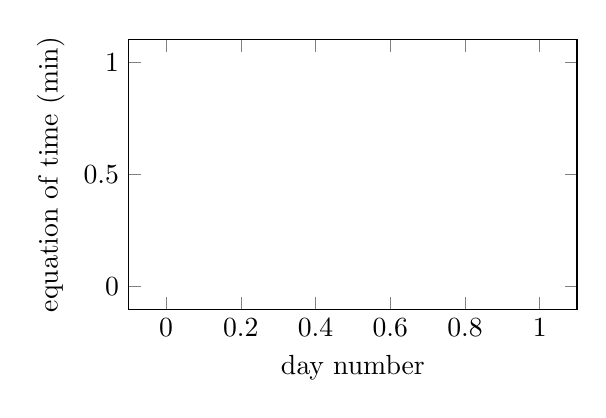
\begin{tikzpicture}
\begin{axis}[height=5cm,
                  width = 0.6\textwidth,
                  xlabel = day number,
                  ylabel = equation of time (min),
                  ]
\addplot[smooth] coordinates {
\equationoftime
};
\end{axis}
\end{tikzpicture}
\end{verbatim}
\end{scriptexample}

Combining the code and inserting it in our document we obtain a nice plot of the equation of time, possibly correct to 12 decimal places.

\begin{figure}[htb]
\begin{scriptexample}{}{}
\bgroup
\centering
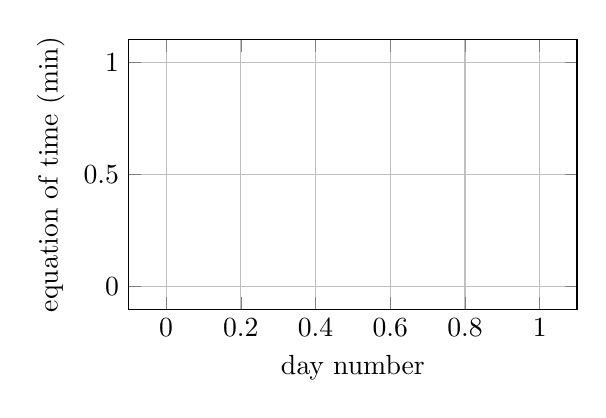
\begin{tikzpicture}
\begin{axis}[height=5cm,
                  width = 0.6\textwidth,
                  xmin = 1, xmax=365,
                  ymax = 15,
                  xlabel = day number,
                  enlarge y limits = true,
                  enlarge x limits = true,
                  ylabel = equation of time (min),
                  grid = major
                  ]
\addplot[smooth] coordinates {
\equationoftime
};
\end{axis}
\end{tikzpicture}

\egroup
\caption{Equation of time, generated via LuaTeX mark-up.}
\end{scriptexample}
\end{figure}

The graph of course still needs a lot of polishing. The axes can have better numbering, we may want to add a title and other enhancements. The one modification which we will do is to make the chart a bit wider and get the x-axis numbering a bit better.  

\begin{figure}[htb]
\begin{scriptexample}{}{}
\bgroup
\centering
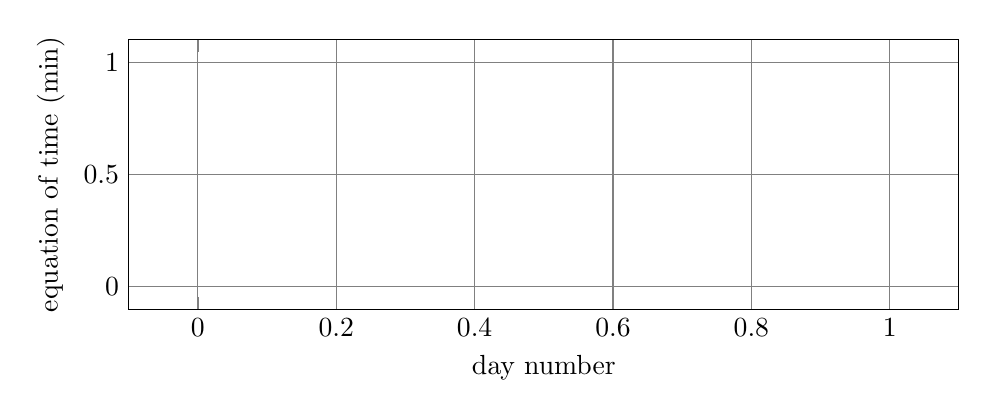
\begin{tikzpicture}
\begin{axis}[height=5cm,
                  width = \textwidth,
                  xmin = 30, xmax=365,
                  ymax = 15,
                  xtick = {30,60,...,360},
                  xlabel = day number,
                  enlarge y limits = true,
                  enlarge x limits = true,
                  ylabel = equation of time (min),
                  grid = major,
                  grid style ={color = black!50},
                  ]
\addplot[smooth] coordinates {
\equationoftime
};
\end{axis}
\end{tikzpicture}

\egroup
\caption{Equation of time, generated via LuaTeX mark-up.}
\end{scriptexample}
\end{figure}

The advantage of having the data the program and the documentation in one document, has major advantages. The generated plots guaranteed that our methods and functions have been tested properly. Of course once we have such a powerful tool in our disposal we can generate from the same routines tabular figures. 



The problem we need to solve is that we need to print the values in rows, one row for each value of the day number for all the months in a year. We also need to cater for all of TeX's mark-up without breaking up anything. Although at first this looks like a difficult task, now that we have sorted the rads from degrees, we need to go back to our module and handle the table from there. It is always easier to generate TeX commands from Lua rather than working from TeX and exporting and importing to Lua.

But how do we organize the code? 


\begin{scriptexample}{}{}
\bgroup
\scriptsize
\begin{luacode}
local c = require("i18n.calendar") 
c.equation_of_time_table ()
\end{luacode}
\captionof{table}{Equation of Time (ET) values for a normal year. }
\egroup
\end{scriptexample}

Modifying the routines to cater for a leap year is fairly simple, we can introduce a variable leap and modify the \docAuxCommand{equation_of_time_table ()} function. 


\bgroup
\footnotesize
\begin{luacode}
local c = require("i18n.calendar") 
c.debug = true
c.equation_of_time_table (true, 12)
\end{luacode}
\captionof{table}{Equation of Time (ET) values for a leap year. }\par

\egroup


The coding of the tables (for the normal year and the leap year) although somewhat unexciting, is important to test that the routines are performing as required, as they provide an easy way to examine the output. As you can observe the day number for both the years are correct. 

It is good practice, that when developing code, you include testing routines and if appropriate also logging routines. The leap table was produced using |c.debug = true|  to view the day number, which was programmed as a subscript to the numerical values of the equation of time.

\subsection{declination}

The declineation angle also takes the day of the year parameter and returns the angle. For this we have already
added a function

%\begin{scriptexample}{}{}
%\begin{luacode}
%local c = require("i18n.calendar")
%c.printdeclination()
%\end{luacode}
%\end{scriptexample}

\section{Solar Constant and Extraterrestrial Solar Radiation}

The solar constant $E_{sc}$ is defined as the intensity of solar radiation
on a surface normal to the sun's rays, just beyond the earth's
atmosphere, at the average earth-sun distance. One frequently used
value is that proposed by the World Meteorological Organization in
1981, $E_{sc} = 1367$W/m2 (Iqbal 1983).


Because the earth's orbit is slightly elliptical, the extraterrestrial
radiant flux E0 varies throughout the year, reaching a maximum
of 1412 W/m2 near the beginning of January, when the earth
is closest to the sun (aphelion) and a minimum of 1322 W/m2 near
the beginning of July, when the earth is farthest from the sun (perihelion).
Extraterrestrial solar irradiance incident on a surface normal
to th


\subsection{Calculating the Solar Azimuth and Altitude}

Now that we have most of the programming behind us, we will calculate the solar azimuth and altitude angles. These require effectively the calling of most of the functions we have coded so far. Once these are calculated then the sunset, zenith and sunrise can be calculated. These will be required later on to build a model for the solar gains and losses of buildings. 

The sun's position in the sky is conveniently expressed in terms
of the solar altitude above the horizontal and the solar azimuth measured
from the south (see Figure 3). The solar altitude angle $\beta$ is
defined as the angle between the horizontal plane and a line emanating
from the sun. Its value ranges from 0° when the sun is on the
horizon, to 90° if the sun is directly overhead. Negative values
correspond to night times. The solar azimuth angle φ is defined as
angular displacement from south of the projection, on the horizontal
plane, of the earth/sun line. By convention, it is counted positive for
afternoon hours and negative for morning hours.


\subsection{Assembling the Model}

The model specification required that from a given location, defined by its latitude and longitude at a particular month, day and time of the year, we should be able to determine the location of the sun on the celestial sphere.

We define an object |location = {latitude, longitude, name}| 












\appendix
\DocInput{\jobname.dtx}
\MakePercentComment
\cxset{palette budapest}

\chapter{ltlists.dtx}
\label{kernel:ltlists}
 \section{List, and related environments}

This section of the kernel is interesting in order to understand the underlying general design
decisions of the \latexe Team.

The kernel source can be considered as a framework, upon which classes build. All \latex lists are aware
of their environment and can be included in other lists. You can also even if you want include sections within
enumerated or itemized lists and they will not break. You can include boxes or minipages. 

This section of the kernel creates generic factory commands for the creation of list environments. 
These list environments \refEnv{enumerate}, \refEnv{itemize} are defined in the kernel, whereas others are normally
defined in the class files (see \vref{ch:bookclass}, \vref{sec:clo} and \vref{sec:booklists}).

To understand how lists are created we need to understand that they are shaped paragraphs. Lamport's 
decision to shape them with \cs{parshape}, has produced a flexible system, used later on by standard classes to create numerous environments. The complexity of the code is necessary to make sure
that at every item the |\parshape| is used and also in any following paragraphs. Remember
that |\parshape| will only act on one paragraph. As Knuth said the \latexe Team did some
nifty tricks with |\parshape|.

A sideline is that the code can be used to add vertical and bottom space to content as well as adjust the left and right margins of text blocks. In the \latexe classes they are used to define the environments for quotations, quotes \vref{sec:quotationenvironment}, verse \autoref{sec:verseenvironment}  and verbatim environments.


\section{Generic Command}

The |\list| is the generic command that is used to create other lists.  Think of it as the |\newcommand|
for new list environments. The command takes two arguments.


\begin{quote}
        |\list|\marg{label}\marg{commands} ... |\endlist|
\end{quote}

 which can be invoked by the user as the |list| environment.  The \meta{label}
 argument specifies item labeling.  \meta{commands} contains commands for
 changing the horizontal and vertical spacing parameters.

 Each item of the environment is begun by the command
 |\item[|item label|]|
 which produces an item labeled by |itemlabel|.  If the argument is
 missing, then the |label| argument of the |\list| command is used as the
 item label. This enables the user to type |item|  or |item[some label]|.

 The label is formed by putting |\makelabel|\marg{ITEMLABEL} in an hbox
 whose width is either its natural width or else |\labelwidth|,
 whichever is larger.  The |\list| command defines \refCom{makelabel} to have
 the default  definition:
 \begin{quote}
     |\makelabel|\marg{arg} == BEGIN |\hfil| arg END
 \end{quote}
 which, for a label of width less than \refCom{labelwidth}, puts the label
 flushright, \refCom{labelsep} to the left of the item's text.  However,
 |\makelabel| can be |\let| to another command by the \refCom{list}'s
\meta{commands} argument.

 A \refCom{usecounter}\marg{foo} command in the second argument causes the
 counter \emph{foo} to be initialized to zero, and stepped by every
 |\item| command without an argument.  (|\label| commands within the
 list refer to this counter.)

 When you leave a list environment, returning either to an enclosing
 list or normal text mode, \latexe begins a new paragraph if and only if
 you leave a blank line after the |\end| command.  This is accomplished
 by the \refCom{@endparenv} command.

 Blank lines are ignored every other reasonable place--i.e.:
 \begin{itemize}
  \item  Between the |\begin{list}| and the first |\item|,
  \item  Between the |\item| and the text of that item.
  \item Between the end of the last item and the |\end{list}|.
 \end{itemize}

 For an environment like \docAuxEnvironment{quotation}, in which items are not labeled,
 the entire environment is a single item.  It is defined by
 letting |\quotation| == |\list{}{...}\item\relax|.  (Note the
 |\relax|, there in case the first character in the environment is a
 '['.)  The spacing parameters provide a great deal of flexability in
 designing the format, including the ability to let the indentation of
 the first paragraph be different from that of the subsequent ones.

 The trivlist environment is equivalent to a list environment
 whose second argument sets the following parameter values:
 \begin{description}
 \item[{\refCom{leftmargin}}] = 0: causes no indentation of left margin
 \item[\refCom{labelwidth} = 0:] see below for precise effect this has.
 \item[\refCom{itemindent} = 0:] with a null label, makes first paragraph
        have no indentation.  Succeeding paragraphs have |\parindent|
        indentation.  To give first paragraph same indentation, set
        |\itemindent| = |\parindent| before the |\item[]|.
 \end{description}

 Every |\item| in a trivlist environment must have an argument---in
 many cases, this will be the null argument (|\item[]|).  The trivlist
 environment is mainly used for paragraphing environments, like
 verbatim, in which there is no margin change.  It provides the same
 vertical spacing as the list environment, and works reasonably well
 when it occurs immediately after an |\item| command in an enclosing
 list.

\begin{texexample}{understanding how lists are being build}{ex:parshape1}

\makeatletter
\def\mybullet{$\bullet$}
\leftskip0pt \rightskip0pt

\newlength\lmargin
\newlength\rmargin
\newlength\lnwidth
\setlength\lnwidth{\linewidth}

\setlength\lmargin{30pt}
\setlength\rmargin{30pt}
\setlength\lnwidth{\textwidth}
\advance\lnwidth-2\rmargin\relax %

\hskip-\lmargin\hbox to \lmargin{\hfill\mybullet}%
\parshape 1 \dimexpr\lmargin\relax \lnwidth\relax
\lorem

% Second list level
\addtolength\lmargin{30pt}\relax
\hskip-\lmargin\hbox to \lmargin{\hfill\mybullet}%
\parshape 1 \dimexpr\lmargin\relax \dimexpr\linewidth-3\rmargin\relax
\lorem

% Third list level
\addtolength\lmargin{30pt}\relax
\hskip-\lmargin\hbox to \lmargin{\hfill\mybullet}%
\parshape 1 \dimexpr\lmargin\relax \dimexpr\linewidth-5\rmargin\relax
\lorem

\makeatother
\end{texexample}

The above were manually defined so that you can understand how the code builds the list. These can be abstracted into a macro similar to |item| to typeset the text. The label can be typeset with a new macro |mklabel|. We will do this first and change it to an enumerated list. I will use a counter that is already defined for this book and use a macro |\inc| to step it up.

\emphasize{mybullet,itm}
\begin{texexample}{understanding how lists are being build}{ex:parshape2}
\makeatletter
\def\mybullet{{\itshape\large\inc. }}
\leftskip0pt \rightskip0pt
\setlength\lmargin{0pt}
\setlength\rmargin{0pt}

\def\itm{%
  \setlength\lmargin{0pt}
  \setlength\rmargin{0pt}
  \hskip-\lmargin\hbox to \lmargin{\hfill\mybullet}%
  \parshape 1 \dimexpr\lmargin\relax \dimexpr\linewidth-\rmargin\relax}

% First level
\itm \lorem

% Second list level
\itm \lorem

% Third list level
\itm \lorem

\makeatother
\end{texexample}

Remember that \latexe defines all lengths to be global lengths, so we didn't have to redeclare them above, just reset them to the values we needed them.


 \subsection{List and Trivlist}

 The following variables are used inside a list environment:
 \begin{description}
 \item[] \refCom{@totalleftmargin} The distance that the prevailing left
     margin is indented from the outermost left margin,
 \item[] \refCom{linewidth} The width of the current line.  Must be
     initialized to |\hsize|.
 \item[] \refCom{@listdepth} A count for holding current list nesting depth.
 
 \item[] \refCom{makelabel} A macro with a single argument, used to
   generate the label from the argument (given or implied)
   of the |\item| command. Initialized to |\@mklab| by the |\list|
   command.  This command must produce  some stretch---i.e., an
   |\hfil|.
   
 \item[] \refCom{if@inlabel} A switch that is false except between the time
   an |\item| is encountered and the time that \TeX{}
   actually enters horizontal mode.  Should be tested by commands
   that can be messed up by the list environment's use of |\everypar|.
   
 \item[] \refCom{@labels} When |@inlabel = true|, it holds the labels
   to be put out by |\everypar|.
   
 \item[] \refCom{if@noparitem} A switch set by |\list| when
   |@inlabel = true|.
      Handles the case of a |\list| being the first thing in an item.
      
 \item[] \refCom{if@noparlist} A switch set true for a list that begins an
   item.  No |\topsep| space is added before or after |\item|'s such a
   list.
   
 \item[] \refCom{if@newlist} Set true by |\list|, set false by the first
   text (by |\everypar|).
   
 \item[]  \refCom{if@noitemarg} Set true when executing an |\item| with no
   explicit argument.  Used to save space. To save time, make two
   separate  \refCom{@item} commands.
   
 \item[] \refCom{if@nmbrlist} Set true by |\usecounter| command, causes
   list to be numbered.
   
 \item[] |noskipsec| A switch set true by a sectioning command when
    it is creating an in-text heading with |\everypar|.
 \end{description}


 Throughout a list environment, |\hsize| is the width of the current
 line, measured from the outermost left margin to the outermost right
 margin.  Environments like tabbing should use \refCom{linewidth} instead of
 |\hsize|.

 Here are the parameters of a list that can be set by commands in
 the |\list|'s \meta{commands} argument.  These parameters are all TeX
 skips or dimensions (defined by |\newskip| or |\newdimen|), so the
 usual \TeX\ or \LaTeX\ commands can be used to set them.  The
 commands will be executed in vmode if and only if the |\list| was
 preceded by a |\par| (or something like an |\end{list}|), so the
 spacing parameters can be set according to whether the list is
 inside a paragraph or is its own paragraph.


 \paragraph{Vertical Spacing (skips)}
 
 \begin{description}
 \item[\refCom{topsep}] Space between first item and preceding paragraph.
 \item[\refCom{partopsep}] Extra space added to \refCom{topsep} when
        environment starts a new paragraph (is called in vmode).
 \item[\refCom{itemsep}] Space between successive items.
 \item[\refCom{parsep}] Space between paragraphs within an item -- the
                 |parskip| for this environment.
 \end{description}

 \paragraph{Penalties}
 
 \begin{description}

 \item[] \refCom{@beginparpenalty} put at the beginning of a list
 \item[] \refCom{@endparpenalty} put at end of list
  \item[] \refCom{@itempenalty} put between items.
  \end{description}

 \subsection{Horizontal Spacing (dimens)}
 \begin{description}
 \item[]  \refCom{leftmargin} space between left margin of enclosing
   environment (or of page if top level list) and left margin of
                     this list.  Must be nonnegative.
  \item[] \refCom{rightmargin} analogous.
  \item[] \refCom{listparindent} extra indentation at beginning of every
     paragraph of a list except the one started by the \refCom{item}
                      command.  May be negative!  Usually, labeled
                       lists have \refCom{listparindent} equal to zero.
   \item[]  \refCom{itemindent} extra indentation added right BEFORE an item
                      label.
  \item[] \refCom{labelwidth} nominal width of box that contains the label.
                      If the natural width of the
                         label $< =$ \refCom{labelwidth},
                      then the label is flushed right inside a box
                      of width \refCom{labelwidth} (with an |\hfil|).
                      Otherwise,
                      a box of the natural width is employed, which
                       causes an indentation of the text on that line.
     \item[] \refCom{labelsep} space between end of label box and text of
                      first item.
  \end{description}


 \subsection{Default Values}
 
 Defaults for the list environment are set as follows.
 First, \refCom{rightmargin}, \refCom{listparindent} and \refCom{itemindent}
 are set
      to 0pt.  Then, one of the commands
      \refCom{@listi}, |@listii|,\ldots,|@listvi|
      is called, depending upon the current level of the list.
      The |@list|\ldots commands should be defined by the document
      style.  A convention that the document style should follow is
      to set \refCom{leftmargin} to
      |leftmargini|,\ldots, |leftmarginiv| for
      the appropriate level.  Items that aren't changed may be left
      alone, but everything that could possibly be changed must be
      reset.


\LinesNumbered
\begin{algorithm}
\caption{The \refCom{list} environment}
  \refCom{list}\marg{LABEL}\marg{COMMANDS} ==\\
   \Begin{
     \eIf{\refCom{@listdepth} > 5}{
        LaTeX error: `Too deeply nested'}{
        \refCom{@listdepth} :=G \refCom{@listdepth} + 1\\
     }
     \refCom{rightmargin}     := 0pt\\
     \refCom{listparindent}   := 0pt\\
     \refCom{itemindent}      := 0pt\\
     eval(@list \refCom{romannumeral}\refCom{the}\refCom{@listdepth})\\  
     \refCom{@itemlabel}      :=L LABEL\\
     \refCom{makelabel}       == \refCom{@mklab}\\
     @nmbrlist :=L false\\
     SETTING COMMANDS\\
     \refCom{@trivlist}\\  
     parskip          :=L \refCom{parsep}\\
     parindent        :=L \refCom{listparindent}\\
     \refCom{linewidth}        :=L \refCom{linewidth} - \refCom{rightmargin} -\refCom{leftmargin}\\
     \refCom{@totalleftmargin} :=L \refCom{@totalleftmargin} + \refCom{leftmargin}\\
     parshape 1 \refCom{@totalleftmargin} \refCom{linewidth}\\
     \cs{ignorespaces} 
   }
\end{algorithm}

The \refCom{endlist} simply adjusts the listdepth counter and ends the \refCom{trivlist}.

\begin{algorithm}
 \refCom{endlist} == \\
  \Begin{
    \refCom{@listdepth} :=G \refCom{@listdepth} -1\\
    \refCom{endtrivlist}\\
  }
\end{algorithm}

The \refCom{@trivlist} is define as,

\begin{algorithm}
 \refCom{@trivlist} ==\\
  \Begin{
    \If{@newlist = T}{\refCom{@noitemerr}}
     This command removed for some forgotten reason.\\
     \refCom{@topsepadd} :=L \refCom{topsep}\\
     \If{@noskipsec}{leave vertical mode}
     \eIf{vertical mode}{
        \refCom{@topsepadd} :=L \refCom{@topsepadd} + \refCom{partopsep}}{
        \cs{unskip} \cs{par}}
     \eIf{@inlabel = true}{
         @noparitem :=L true
         @noparlist :=L true}{
         @noparlist :=L false
             \refCom{@topsep}   :=L \refCom{@topsepadd}}
     \refCom{@topsep}      :=L \refCom{@topsep} + \refCom{parskip}\\
      Restore paragraphing parameters\\
     \cs{leftskip}     :=L 0pt\\  
     \cs{rightskip}    :=L \refCom{@rightskip}\\
     \cs{parfillskip}     :=L 0pt + 1fil\\
   NOTE: \cs{@setpar} called on every \refCom{list} in case \cs{par} has been\\
   temporarily  munged before the \refCom{list} command.\\
     \cs{@setpar}{if @newlist = false then {\cs{@@par}} fi}\\
     \refCmd{@newlist}         :=G T\\
     \refCmd{@outerparskip}    :=L \cs{parskip}\\
 }
\end{algorithm}

\begin{algorithm}
 \refCom{trivlist}  ==\\
 \Begin{
  \refCom{parsep} := \cs{parskip}\\
  \cs{@nmbrlist} := false\\
  \refCom{@trivlist}\\
  \refCom{labelwidth} := 0\\
  \refCom{leftmargin} := 0\\
  \refCom{itemindent} := \refCom{parindent}\\
  \refCom{@itemlabel} :=L "empty"\\ 
  \refCom{makelabel}\marg{LABEL} == LABEL\\
 }
\end{algorithm}



\begin{algorithm}
 \refCom{endtrivlist} ==\\
 \Begin{
     \If{@inlabel = T}{\refCom{indent}}
     \If{horizontal mode}{\refCom{unskip} \refCom{par}}
     \eIf{@noparlist = true}{}{
        \If{\refCom{lastskip} > 0}{
              \refCom{@tempskipa} := \refCom{lastskip}
              \refCom{vskip} - \refCom{lastskip}
              \refCom{vskip} \refCom{@tempskipa} -\refCom{@outerparskip} + \refCom{parskip}
             }
           \refCom{@endparenv}
     }
   }
\end{algorithm}


\begin{algorithm}
 \refCom{@endparenv} ==
   \Begin{
    \refCom{addpenalty}\marg{@endparpenalty}\\
    \refCom{addvspace}\marg{\refCom{@topsepadd}}\\
     ends the \refCom{begin} command's \refCom{begingroup}\\
    \cs{endgroup}\\
    \cs{par}  ==  \Begin{%
                  \refCom{@restorepar}\\
                  \cs{everypar}|{}|
                  \cs{par}
                  }
    \refCom{everypar} == \Begin{remove \refCom{lastbox} \refCom{everypar}|{}|}
   to match the \refCom{end} commands \refCom{endgroup}\\
    \refCom{begingroup}  
   }
\end{algorithm}

\index{kernel>lists>\textbackslash item}
The definition of item, is fairly simple deferring the complexity
to \refCom{@item} which follows.

\begin{algorithm}[htbp]
 \refCom{item} == \Begin{
    \If{math mode}{issue warning}
    \eIf{ next char = {\tt [}}{
             \refCom{@item}}{
              @noitemarg := true\\
             \refCom{@item}[\refCom{@itemlabel}]}
  }
\caption{The algorithm for \textbackslash item}
\end{algorithm}


\begin{algorithm}
 \refCom{@item}[LAB] ==
    \Begin{
     \eIf{@noparitem = true}{
        @noparitem := false
             % NOTE: then clause  hardly every taken,\\
             %  so made a macro \refCom{@donoparitem}\\
            \refCom{box}\refCom{@labels} :=G\\
             \refCom{hbox} \Begin{hskip -\refCom{leftmargin}\\
                                   {box}   \\refCom{@labels}\\
                                   {hskip} \refCom{leftmargin}}
            \If{@minipage = false}{
               \refCom{@tempskipa} := \refCom{lastskip}\\
               \refCom{vskip} -\refCom{lastskip}\\
               \refCom{vskip} \refCom{@tempskipa} + \refCom{@outerparskip} - \refCom{parskip}}
            }{
          \If{@inlabel = true}{
              then \refCom{indent} \refCom{par}   % previous item empty.
           }
           \If{hmode}{then 2 \refCom{unskip}'s\\
                           % To remove any space at end of prev.\\
                           % paragraph that could cause a blank line.\\
                     \refCom{par}\\
           }
           \eIf{if @newlist = T}{
                \eIf{@nobreak = T}{ 
                      % Kludge if list follows \refCom{section}\\
                      \refCom{addvspace}\marg{\refCom{@outerparskip} - \refCom{parskip}}}{
                       \refCom{addpenalty}\marg{\refCom{@beginparpenalty}}\\
                       \refCom{addvspace}\marg{\refCom{@topsep}}\\
                       \refCom{addvspace}\marg{-\refCom{parskip}}\\  
                    }}{
                \refCom{addpenalty}\marg{\refCom{@itempenalty}}\\
                \refCom{addvspace}\marg{\refCom{itemsep}}\\
            }

            @inlabel :=G true\\
     }

     \refCom{everypar}\{ @minipage :=G F\\
                @newlist :=G F\\
                \If{@inlabel = true}{
                    @inlabel :=G false
                       \refCom{hskip} -\refCom{parindent}\\
                       \refCom{box}\refCom{@labels}\\
                       \refCom{penalty} 0\\
                       \refCom{box}\refCom{@labels} :=G null\\
                }
                \refCom{everypar}\{\} \}\\
     @nobreak :=G false\\
     \If{@noitemarg = true}{
        @noitemarg := false\\
            \If{@nmbrlist}{
               \refCom{refstepcounter}\{\refCom{@listctr}\}
            }
     }
     \refCom{@tempboxa}   :=L \refCom{hbox}\marg{\refCom{makelabel}\marg{LAB}}\\
     \refCom{box}\refCom{@labels} :=G \refCom{@labels}\refCom{hskip}\refCom{itemindent}\\
                       \refCom{hskip} - (\refCom{labelwidth} + \refCom{labelsep})\\
                 \eIf{\refCom{wd}\refCom{@tempboxa} > \refCom{labelwidth}}{
                          \refCom{box}\refCom{@tempboxa}}{
                          \refCom{hbox} to \refCom{labelwidth}\{\refCom{unhbox}\refCom{@tempboxa}\}\\
                 } 
      \refCom{hskip}\refCom{labelsep}\\
     \refCom{ignorespaces} %gobble space up to text
  }
\end{algorithm}




\begin{algorithm}
 \refCom{makelabel}\marg{LABEL} == ERROR\\
    default to catch lonely \refCom{item}

 \refCom{usecounter}\marg{CTR} == \Begin{
                              @nmbrlist :=L true\\
                              @listctr == CTR\\
                              setcounter\marg{CTR}\marg{0}
                             }
\end{algorithm}



 

\begin{docCommand}{topsep} {\meta{dim}}
The space between the first item and the preceding paragraph.
\end{docCommand}

\begin{docCommand}{partopsep} {\meta{dim}}
The space between the first item and the preceding paragraph.
\end{docCommand}

\begin{docCommand}{itemsep} {\meta{dim}}
The space between the first item and the preceding paragraph.
\end{docCommand}

\begin{docCommand}{@itemsep} {\meta{dim}}
The space between the first item and the preceding paragraph.
\end{docCommand}

\begin{docCommand}{@topsepadd} {\meta{dim}}
The space between the first item and the preceding paragraph.
\end{docCommand}

\begin{docCommand}{outerparskip} {\meta{dim}}
The space between the first item and the preceding paragraph.
\end{docCommand}

\begin{docCommand}{parsep} {\meta{dim}}
The space between the first item and the preceding paragraph.
\end{docCommand}

The skip registers \docAuxCommand{topskip}, \docAuxCommand*{partopsep}, 
\docAuxCommand{itemsep}, \docAuxCommand{parsep}, \docAuxCommand{@topsep},
\docAuxCommand{@topsepadd}, \docAuxCommand{outerparskip} are created.

    \begin{teX}
\newskip\partopsep
\newskip\itemsep
\newskip\parsep
\newskip\@topsep
\newskip\@topsepadd
\newskip\@outerparskip
    \end{teX}
 
 
\begin{docCommand}{leftmargin} {\meta{dim}}
|\newdimen\leftmargin|
\end{docCommand}

\begin{docCommand}{rightmargin} {\meta{dim}}
|\newdimen\rightmargin|

\end{docCommand}

\begin{docCommand}{listparindent} {\meta{dim}}
|\newdimen\listparindent|
\end{docCommand}

\begin{docCommand}{labelwidth} {\meta{dim}}
|\newdimen\labelwidth|
\end{docCommand}


\begin{docCommand}{labelsep} {\meta{dim}}
 |\newdimen\labelsep|
\end{docCommand}

\begin{docCommand}{linewidth} {\meta{dim}}
|\newdimen\linewidth|
\end{docCommand}

\begin{docCommand}{itemindent} {\meta{dim}}
|\newdimen\itemindent|
\end{docCommand}

\begin{docCommand}{@totalleftmargin} {\meta{dim}}
|\newdimen\@totalleftmargin|  |\@totalleftmargin=\z@|
\end{docCommand}


 
\begin{docCommand} {leftmargini} { \meta{dim}}
\end{docCommand}
\begin{teX}
\newdimen\leftmargini
\end{teX}
\begin{docCommand} {leftmarginii} { \meta{dim}}
\end{docCommand}
\begin{teX}
\newdimen\leftmarginii
\end{teX}

\begin{docCommand} {leftmarginiii} { \meta{dim}}
\end{docCommand}
\begin{teX}
\newdimen\leftmarginiii
\end{teX}

\begin{docCommand} {leftmarginiv} { \meta{dim}}
\end{docCommand}
\begin{teX}
\newdimen\leftmarginiv
\end{teX}
    \begin{teX}
\newdimen\leftmarginv
    \end{teX}


\begin{docCommand}{@listdepth}{}
\end{docCommand}
\begin{docCommand}{@itempenalty}{}
\end{docCommand}
\begin{docCommand}{@beginparpenalty}{}
\end{docCommand}
\begin{docCommand}{@endparpenalty}{\meta{penalty}}
|\newcount\@endparpenalty|
\end{docCommand}
    \begin{teX}
\newcount\@listdepth \@listdepth=0
\newcount\@itempenalty
\newcount\@beginparpenalty

    \end{teX}


 \begin{docCommand}{@labels} { \meta{box} }
 \end{docCommand}
    \begin{teX}
\newbox\@labels
    \end{teX}
 


 \begin{docCommand}{if@inlabel}{}
   \docAuxCommand{@inlabel}true and false 
  \end{docCommand}
    \begin{teX}
\newif\if@inlabel \@inlabelfalse
    \end{teX}



\begin{docCommand}{ if@newlist} { }
\end{docCommand}
  \begin{teX}
\newif\if@newlist   \@newlistfalse
    \end{teX}
  
  \begin{docCommand}{if@newlistfalse }{}
  \end{docCommand}
  \begin{docCommand}{if@newlisttrue }{}
  \end{docCommand}
 
  
 
\begin{docCommand}{if@noparitem}{}
 \end{docCommand}
 \begin{docCommand}{ if@noparitemtrue}{}
 \end{docCommand}
 \begin{docCommand}{ if@noparitemfalse}{}
 \end{docCommand}
 
\begin{teX}
\newif\if@noparitem \@noparitemfalse
\end{teX}
 

\begin{docCommand} {if@noparlist} { }
  \end{docCommand}
  
\begin{docCommand} {if@noparlistfalse}{}
\end{docCommand}

\begin{docCommand} {if@noparlisttrue}{}
\end{docCommand}  
  
\begin{teX}
\newif\if@noparlist \@noparlistfalse
\end{teX}


\begin{docCommand} {if@noitemarg} { }
\end{docCommand}

\begin{docCommand}{if@noitemargtrue}{}
\end{docCommand}  

\begin{docCommand}{if@noitemargfalse}{}
\end{docCommand}  

    \begin{teX}
\newif\if@noitemarg \@noitemargfalse
    \end{teX}


\begin{docCommand}{if@newlist}{}
\end{docCommand}

\begin{docCommand}{if@newlisttrue}{}
\end{docCommand}  

\begin{docCommand}{if@newlistfalse}{}
   \docAuxCommand{@newlist}
\end{docCommand}  

\begin{docCommand}{if@nmbrlist}{}
Checks if the list is to be numbered or not
\end{docCommand}
  
\begin{teX}
\newif\if@nmbrlist  \@nmbrlistfalse
\end{teX}




\begin{docCommand} {@itemlabel} { }
  Temporary definition to store the label.
\end{docCommand}

\section{The \textbackslash list environment}

Notice that the list takes two arguments the first parameter contains instructions as to how
to typeset items, that do not have an |\item[]|. If we need to step a counter we tell it here


\begin{texexample}{The list}{k:list}
\@ifundefined{c@steps}{\newcounter{steps}}{}
\begin{list}{\bfseries\upshape Step \arabic{steps}:}
{%
\usecounter{steps}
\setlength{\labelwidth}{2cm}\setlength{\leftmargin}{2.6cm}
\setlength{\labelsep}{0.5cm}\setlength{\rightmargin}{1cm}
\setlength{\parsep}{0.5ex plus0.2ex minus0.1ex}
\setlength{\itemsep}{0ex plus0.2ex minus0pt}\relax \slshape %
}
\item Understand how they are being build
\item Define your own environment
\item[Has Own] test
\end{list}


\newenvironment{myplain}
{ 
  \list{\bfseries\arabic{steps} }{\usecounter{steps}\bfseries } }
 {\endlist}


\begin{myplain}
\item \lorem

\item[Something]  \lorem
\end{myplain}
\end{texexample}

Looking at the |list| environement differntly it is actually a settings environment, it sets what to do if the item has nor argument and also sets the counter to be used the current levels. It end issuing a parshape command that is going to
shape the paragraph that follows. Next we need to see how item works in more detail. The calculations and some of the work is
delegated to trivlist.

The code follows:


\index{kernel>lists>\textbackslash list}
\begin{docCommand} {list} {\marg{item label } \marg {commands} }
 List takes two arguments and is factory command for building
other lists.
\end{docCommand}


Check that the list is not nested too far.
 
    \begin{teX}
\def\list#1#2{%
  \ifnum \@listdepth >5\relax
    \@toodeep
  \else
    \global\advance\@listdepth\@ne
  \fi
   \end{teX}
Initialize all margins to 0pt in case the user did not specify anything.   
   \begin{texcode}{}{}  
  \rightmargin\z@
  \listparindent\z@
  \itemindent\z@
  \csname @list\romannumeral\the\@listdepth\endcsname
   \end{teX}

Define the item label here, if it is empty it will be defined to empty   
   \begin{texcode}  
   % store the itemlabel 
  \def\@itemlabel{#1}%
  \let\makelabel\@mklab
  \@nmbrlistfalse
  % insert other parameters, spaces, fonts etc
   #2\relax
  % call trivlist to do some calculations
  % and set conditionals 
  \@trivlist
  
  % redefine parskip and parindent
  \parskip\parsep
  \parindent\listparindent
  
  % set the linewidth
  \advance\linewidth -\rightmargin
  \advance\linewidth -\leftmargin
  \advance\@totalleftmargin \leftmargin
  \end{texcode}
  
  Finally set the parshape commands. Thsi is perhaps the most misunderstood line in the whole
  routine. As you see we cannot do any typsetting as yet. Both parameters are just commands to be
  entered before the text, is typeset. Probably you guessed, but what follows is |\item|. At this
  point it will just activate an error if it is missing.  
  \begin{teX}  
  \parshape \@ne \@totalleftmargin \linewidth
  \ignorespaces}
    \end{teX}


\begin{docCommand}{par@deathcycles}{}
\end{docCommand}
    \begin{teX}
\newcount\par@deathcycles
    \end{teX}
 

 \begin{docCommand}{@trivlist}{}
   Auxiliary macro call by trivlist.
 \end{docCommand}
  Because |\par| is sometimes made a no-op it is possible for a missing
 |\item| to produce a loop that does not fill memory and so never gets
 trapped by \TeX.  We thus need to trap this here by seting |\par| to
 count the number of times a paragraph ii is called with no progress
 being made started.
    \begin{teX}
\def\@trivlist{%
  \if@noskipsec \leavevmode \fi
  \@topsepadd \topsep
  \ifvmode
    \advance\@topsepadd \partopsep
  \else
    \unskip \par
  \fi
  \if@inlabel
    \@noparitemtrue
    \@noparlisttrue
  \else
    \if@newlist \@noitemerr \fi
    \@noparlistfalse
    \@topsep \@topsepadd
  \fi
  \advance\@topsep \parskip
  \leftskip \z@skip
  \rightskip \@rightskip
  \parfillskip \@flushglue
  \par@deathcycles \z@
  \@setpar{\if@newlist
             \advance\par@deathcycles \@ne
             \ifnum \par@deathcycles >\@m
               \@noitemerr
               {\@@par}%
             \fi
           \else
             {\@@par}%
           \fi}%
  \global \@newlisttrue
  \@outerparskip \parskip}
    \end{teX}

The function of a |trivlist| is very simple, it sets numbering to false and initializes all  widths to zero, thus at this stage it will default to a normal paragraph then it calls the auxiliary function \refCom{@trivlist}, which will set
the top and bottom skips and other paragraphing parameters, if set.

\begin{texexample}{Trivlist}{ex:trivlist}
\lorem
\begin{trivlist}
\item[] \lorem

\end{trivlist}
\lorem

\end{texexample}

 \begin{docCommand}{trivlist} { \meta{void} }
 \end{docCommand} 
     \begin{teX}
\def\trivlist{%
  \parsep\parskip
  \@nmbrlistfalse
  \@trivlist
  \labelwidth\z@
  \leftmargin\z@
  \itemindent\z@
    \end{teX}

    We initialise |\@itemlabel| so that a \texttt{trivlist} with
    an |\item| not having an optional argument doesn't produce an
    error message.

 \begin{docCommand} {makelabel} {\marg{item label}}
 \end{docCommand}
    \begin{teX}
  \let\@itemlabel\@empty
  \def\makelabel##1{##1}}
    \end{teX}


 \begin{docCommand}{endlist} {  \meta{void}}
  ends the list environment
 \end{docCommand}
     \begin{teX}
\def\endlist{%
  \global\advance\@listdepth\m@ne
  \endtrivlist}
    \end{teX}
 

    The definition of \refCom{trivlist} used to be in ltspace.dtx 
    so that other commands could be `let to it'.  
    They now use \refCom{def}.
 \begin{docCommand}{endtrivlist}{}
 \end{docCommand}
 
% \changes{v1.2b ltspace}{1994/11/12}{Changed order of tests to make
% \refCom{@noitemerror} correct: end of an era.}
% \changes{v1.0i}{1995/05/25}{Macros moved from ltspace.dtx}
% \changes{v1.0n}{1996/10/25}{Change \refCom{indent} to \refCom{leavevmode}}
% \changes{v1.0n}{1996/10/25}{Reset flags explicitly}
% \changes{v1.0o}{1996/10/26}{Correct typo}
    \begin{teX}
\def\endtrivlist{%
  \if@inlabel
    \leavevmode
    \global \@inlabelfalse
  \fi
  \if@newlist
    \@noitemerr
    \global \@newlistfalse
  \fi
  \ifhmode\unskip \par
    \end{teX}
    We also check if we are in math mode and issue an error message
    if so (hoping that |\@currenvir| resolves suitably). Otherwise
    the usual ``perhaps a missing item'' error will get triggered
    later which is confusing.
 \changes{v1.0s}{2002/10/28}{Check for math mode (pr/3437)}
    \begin{teX}
  \else
    \@inmatherr{\end{\@currenvir}}%
  \fi
  \if@noparlist \else
    \ifdim\lastskip >\z@
      \@tempskipa\lastskip \vskip -\lastskip
      \advance\@tempskipa\parskip \advance\@tempskipa -\@outerparskip
      \vskip\@tempskipa
    \fi
    \@endparenv
  \fi
}
    \end{teX}
 

  \begin{docCommand}{@endparenv}{}
 \end{docCommand}
 
     \begin{teX}
\def\@endparenv{%
  \addpenalty\@endparpenalty\addvspace\@topsepadd\@endpetrue}
    \end{teX}


 
\begin{docCommand}{@doendpe}{}
   To suppress the paragraph indentation in text immediately following
   a paragraph-making environment, \cs{everypar} is changed to remove the
   space, and \cs{par} is redefined to restore \cs{everypar}.  Instead of
   redefining \refCom{par} and \cs{everypar}, \refCom{@endparenv} was changed to 
   set the \refCom{@endpe} switch, letting |end| redefine |par| and 
   |everypar|.   This allows paragraph-making environments to work right when called 
 by other environments. )
\end{docCommand}
 

    \begin{teX}
\def\@doendpe{\@endpetrue
     \def\par{\@restorepar\everypar{}
          \par\@endpefalse}\everypar
          {{\setbox\z@\lastbox}\everypar{}\@endpefalse}}
    \end{teX}
    
    Use |\setbox0=\lastbox| instead of   |\hskip -\parindent|   
    so that a |\noindent| becomes a no-op when used before 
    a line immediately following a list environment(23 Oct 86).
 \changes{v1.0k}{1995/11/07}{Enclosed \refCom{setbox0} assignment by a
 group so that it leaves the contents of box $0$ intact.
    }

  \begin{docCommand}{if@endpe}{}
 \end{docCommand}
  \begin{docCommand}{@endpelttrue}{}
 \end{docCommand}
% \begin{macro}{\if@endpe}
% \begin{macro}{\@endpefalse}
% \begin{macro}{\@endpeltrue}
    \begin{teX}
\newif\if@endpe
\@endpefalse
    \end{teX}
% \end{macro}\end{macro}\end{macro}

 \begin{docCommand}{@mklab}{}
 \end{docCommand}
    \begin{teX}
\def\@mklab#1{\hfil #1}
    \end{teX}

 \changes{LaTeX2.09}{1992/09/18}
     {(RmS) Added warning if \refCom{item} is used in math mode}
 \changes{v1.0c}{1994/04/28}
     {Replaced \refCom{@ltxnomath} by \refCom{@inmatherr}}
 \changes{v1.0d}{1994/05/03}
     {Removed superfluous braces}
     
\section{Typesetting the label}     
 
 \begin{docCommand}{item}{\oarg{label}}
 
 \end{docCommand}     
 
 
     \begin{teX}
\def\item{%
  \@inmatherr\item
  \@ifnextchar [\@item{\@noitemargtrue \@item[\@itemlabel]}}
    \end{teX}
 
 \begin{docCommand} {@donoparitem} { }
 \end{docCommand}
    \begin{teX}
\def\@donoparitem{%
  \@noparitemfalse
  \global\setbox\@labels\hbox{\hskip -\leftmargin
                               \unhbox\@labels
                                \hskip \leftmargin}%
  \if@minipage
    \else
      \@tempskipa\lastskip
      \vskip -\lastskip
      \advance\@tempskipa\@outerparskip
      \advance\@tempskipa -\parskip
      \vskip\@tempskipa
  \fi}
    \end{teX}

 
 \begin{docCommand}{@item}{\marg{label} }
 \end{docCommand}
 
     \begin{teX}
\def\@item[#1]{%
  \if@noparitem
    \@donoparitem
  \else
    \if@inlabel
      \indent \par
    \fi
    \ifhmode
      \unskip\unskip \par
    \fi
    \if@newlist
      \if@nobreak
        \@nbitem
      \else
        \addpenalty\@beginparpenalty
        \addvspace\@topsep
        \addvspace{-\parskip}%
      \fi
    \else
      \addpenalty\@itempenalty
      \addvspace\itemsep
    \fi
    \global\@inlabeltrue
  \fi
  \everypar{%
    \@minipagefalse
    \global\@newlistfalse
    \end{teX}
    This |\if@inlabel| check is needed in case an item starts of
    inside a group so that |\everypar| does not become empty
    outside that group. 
 \@nobreakfalse, etc etc.
    \begin{teX}
    \if@inlabel
      \global\@inlabelfalse
    \end{teX}
    The paragraph indent is now removed by using |\setbox...| since
    this makes |\noindent| a no-op here, as it should be. Thus the
    following comment is redundant but is left here for the sake of
    future historians:
    this next command was changed from an hskip to a kern to avoid
    a break point after the parindent box: the skip could cause a
    line-break if a very long label occurs in raggedright setting.
 \changes{v1.0d}{1994/05/03}{\refCom{hskip} changed to \refCom{kern}}
 \changes{v1.0m}{1996/10/23}{\refCom{kern...} changed to \refCom{setbox...}}
 \changes{v1.0r}{1997/02/21}
    {\refCom{ifvoid} check added for \refCom{noindent}. latex/2414}
 If |\noindent| was used after |\item| want to cancel the |\itemindent|
 skip. This case can be detected as the indentation box will be void.
    \begin{teX}
      {\setbox\z@\lastbox
       \ifvoid\z@
         \kern-\itemindent
       \fi}%
    \end{teX}

    \begin{teX}
      \box\@labels
      \penalty\z@
    \fi
    \end{teX}
    This code is intended to prevent a page break after the first
    line of an item that comes immediately after a section title. It
    may be sensible to always forbid a page break after one line of
    an item?  As with all such settings of |\clubpenalty| it is local
    so will have no effect if the item starts in a group.

    Only resetting |\@nobreak| when it is true is now
    essential since now it is sometimes set locally.
 \changes{v1.0m}{1996/10/23}{Added setting of \refCom{clubpenalty} and
    set \refCom{@nobreakfalse} only when necessary}
    \begin{teX}
    \if@nobreak
      \@nobreakfalse
      \clubpenalty \@M
    \else
      \clubpenalty \@clubpenalty
      \everypar{}%
    \fi}%
    \end{teX}
 \changes{v1.0l}{1996/07/26}{Remove unecessary \refCom{global} before
                 \refCom{@nobreak...}}
 \changes{v1.0m}{1996/10/23}{\refCom{@nobreak...} moved into the
          \refCom{everypar} and not executed unconditionally, see above} 
    \begin{teX}
  \if@noitemarg
    \@noitemargfalse
    \if@nmbrlist
    \end{teX}
 \changes{v1.0g}{1995/05/17}{Removed surplus braces}
    \begin{teX}
      \refstepcounter\@listctr
    \fi
  \fi
    \end{teX}
    
Before the label is typeset it is placed in a bo. The latex Team used an |\sbox| so that colour commands can be supported.
It call |\makelabel| with the item parameters.

    \begin{teX}
  \sbox\@tempboxa{\makelabel{#1}}%
  \global\setbox\@labels\hbox{%
    \unhbox\@labels
    \hskip \itemindent
    \hskip -\labelwidth 
    \hskip -\labelsep
    \ifdim \wd\@tempboxa >\labelwidth
       \box\@tempboxa
\end{teX}

\begin{teX}
%
% \changes{LaTeX2.09}{1991/11/22}
%         {(RmS) Changed second call to \refCom{makelabel} to
%           \refCom{unhbox}\refCom{@tempboxa}.
%          Avoids problems with side effects in \refCom{makelabel} and is
%               more efficient.}
%    \begin{teX}
    \else
      \hbox to\labelwidth {\unhbox\@tempboxa}%
    \fix
    \hskip \labelsep}%
  \ignorespaces}
    \end{teX}
 
 
 
 
 \begin{docCommand}{makelabel}{}
 Initial definition of \cs{makelabel} set to produce the infamous and often encountered error, if it
 has not been defined by one of the paragraphing environments.
 \end{docCommand}
 
    \begin{teX}
\def\makelabel#1{%
  \@latex@error{Lonely \string\item--perhaps a missing
        list environment}\@ehc}
    \end{teX}
 

 \begin{docCommand}{nbitem}{}
 \end{docCommand}
% \begin{macro}{\@nbitem}
 \changes{v1.0g}{1995/05/17}{Removed surplus braces}
    \begin{teX}
\def\@nbitem{%
  \@tempskipa\@outerparskip
  \advance\@tempskipa -\parskip
  \addvspace\@tempskipa}
    \end{teX}

 \begin{docCommand}{usecounter}{}
 \end{docCommand}
    \begin{teX}
\def\usecounter#1{\@nmbrlisttrue\def\@listctr{#1}\setcounter{#1}\z@}
    \end{teX}


 \section{Enumerate}

  Enumeration is done with four counters: |enumi|, |enumii|, |enumiii|
  and |enumiv|, where |enum|N controls the numbering of the Nth level
  enumeration.  The label is generated by the commands
  \refCom{labelenumi} \ldots{} \cs{labelenumiv}, which should be defined
  by the document style.
  
  Note that \cs{p@enum}N \cs{theenum}N defines the output
  of a \refCom{ref} command.  A typical definition might be:
  
 \begin{verbatim}
     \def\theenumii{\alph{enumii}}
     \def\p@enumii{\theenumi}
     \def\labelenumii{(\theenumii)}
 \end{verbatim}
 which will print the labels as `(a)', `(b)', \ldots
 and print a \refCom{ref} as `3a'.

 The item numbers are moved to the right of the label box, so they are
 always a distance of \refCom{labelsep} from the item.

 \refCom{@enumdepth} holds the current enumeration nesting depth.

 Itemization is controlled by four commands: \docAuxCommand{labelitemi},
 \docAuxCommand{labelitemii},
 \docAuxCommand{labelitemiii}, and \docAuxCommand{labelitemiv}.
 To cause the second-level list to be
 bulleted, you just define \docAuxCommand{labelitemii}
 to be |$\bullet$|.  |@itemspacing|
 and \refCom{@itemdepth} are the analogs of |@enumspacing| and
 \refCom{@enumdepth}. These are not defined in the kernel, their definition is delegated to the classes and to another extend to the users.


 \begin{docCommand}{@enumdepth}{}
  The enumeration depth. 
 \end{docCommand}
     \begin{teX}
\newcount\@enumdepth \@enumdepth = 0
    \end{teX}
 

Next the counters for the \refEnv{enumerate} environment, \docCounter{c@enumi}, \docCounter{c@enumii}, \docCounter{c@enumiii} and \docCounter{c@enumiv} are created.

    \begin{teX}
 \@definecounter{enumi} 
 \@definecounter{enumii} 
 \@definecounter{enumiii} 
 \@definecounter{enumiv}
    \end{teX}


 \begin{docEnvironment}{enumerate}{}{}
 \end{docEnvironment}  
   The enumerate environment enumerates the list. The macro
  is written very efficiently and defines the basic structure. The
  typesetting parameters are left for the class files such as book
  to define them.

     \begin{teX}
 \def\enumerate{%
  \ifnum \@enumdepth >\thr@@\@toodeep\else
    \advance\@enumdepth\@ne
    \edef\@enumctr{enum\romannumeral\the\@enumdepth}%
      \expandafter
      \list
         \csname label\@enumctr\endcsname
        {\usecounter\@enumctr\def\makelabel##1{\hss\llap{##1}}}%
  \fi}
    \end{teX}

    \begin{teX}
 \let\endenumerate =\endlist
    \end{teX}

 \begin{docCommand}{@itemdepth}{}
 \end{docCommand}
    \begin{teX}
\newcount\@itemdepth \@itemdepth = 0
    \end{teX}

\section{The itemize environment}

Finally the \docValue{itemize} environment is defined. This is defined in the kernel to have a limit of 4 levels only.

Itemization is controlled by four commands, which are defined in the standard classes: |\labelitemi|,
   |\labelitemii|, |\labelitemiii|, and |\labelitemiv|, which define
    the labels of the various itemization levels: the symbols used in the standard classes are
    bullet, bold en-dash, centered asterisk and centred dot.



\begin{docEnvironment}{itemize}{}
\end{docEnvironment}


     \begin{teX}
 \def\itemize{%
  \ifnum \@itemdepth >\thr@@\@toodeep\else
    \advance\@itemdepth\@ne
    \edef\@itemitem{labelitem\romannumeral\the\@itemdepth}% (*@\dcircle{1}@*)
    \end{teX}

The \dcircle{1} is a hack to create the |\@itemi|\ldots|\@itemv| names. How it works is that the
|\romannumeral| will expand until it finds a number and leave the letter |i| etc. in the stream.

\begin{texexample}{Creating a suffix with Roman Numerals}{ex:rmnumeral}
\newcounter{tempcounter}
\setcounter{tempcounter}{5}
\edef\itemtest{labelitem\romannumeral\thetempcounter}
%  the replacement
\meaning\itemtest

\itemtest
\end{texexample}
    
    
A romannumeral just returns nothing if it encounters the number \texttt{0} or a negative number. 

\begin{texexample}{Creating a suffix with Roman Numerals}{ex:rmnumeral1}
% counter has been created globally
% commented out.
%\newcounter{tempcounter}
\setcounter{tempcounter}{0}
\edef\itemtest{labelitem\romannumeral\thetempcounter}
%  the replacement
\meaning\itemtest\par
\itemtest
\end{texexample}
    
    
Call the \refCom{list} sets all parameters and defines a  \refCom{makelabel} for this particular
environment. This is a good place to also hook other items to decorate the label, if necessary.
Remember also that the \docAuxCommand{@itemitem}, defined above is just there to facilitate  
calling |labelitemi| \ldots |labelitemn| depending on the level.

\begin{teX}[numbers=none]
    \expandafter
    \list
      
      \csname\@itemitem\endcsname
      {\def\makelabel##1{\hss\llap{##1}}}%
  \fi}
\end{teX}

The astude reader will notice at this point that although we defined the name of labeli etc, they still have no meaning. As mentioned earlier there is still some work to be done before we have full lists. These are defined in the standatrd classes and the definitions are shown below.\tcbdocmarginnote{revised\\13-06-2018}

\begin{teX}
\newcommand\labelitemi{\textbullet}
\newcommand\labelitemii{\normalfont\bfseries \textendash}
\newcommand\labelitemiii{\textasteriskcentered}
\newcommand\labelitemiv{\textperiodcentered}
\end{teX}

Finally the end of the environment is defined.

    \begin{teX}
\let\enditemize =\endlist
    \end{teX}




\chapter{The classes module}
\cxset{palette spring onion}
\begin{teX}
%<article|report|book>\NeedsTeXFormat{LaTeX2e}[1995/12/01]
\end{teX}
%
%    Announce the Class name and its version:
\begin{teX}
%<article>\ProvidesClass{article}
%<report>\ProvidesClass{report}
%<book>\ProvidesClass{book}
%<10pt&!bk>\ProvidesFile{size10.clo}
%<11pt&!bk>\ProvidesFile{size11.clo}
%<12pt&!bk>\ProvidesFile{size12.clo}
%<10pt&bk>\ProvidesFile{bk10.clo}
%<11pt&bk>\ProvidesFile{bk11.clo}
%<12pt&bk>\ProvidesFile{bk12.clo}
%<*driver>
\ProvidesFile{classes.drv}
%</driver>
              [2014/09/29 v1.4h
%<article|report|book> Standard LaTeX document class]
%<10pt|11pt|12pt>      Standard LaTeX file (size option)]
\end{teX}
%
\section{A driver for this document}

 The next bit of code contains the documentation driver file for
 \TeX{}, i.e., the file that will produce the documentation you are
 currently reading. It will be extracted from this file by the
 {\sc docstrip} program.

% \changes{1.0f}{1993/12/07}{Use class ltxdoc document class}
% \changes{1.0r}{1994/02/28}{Moved driver code in order not to need a
%    separate driver}

%
% \changes{v1.0d}{1993/11/30}{remove \cs{@in}, made option makeindex
%    a synonym for option makeidx}
% \changes{v1.0d}{1993/11/30}{removed \cs{@minus}, \cs{@plus},
%    \cs{@settopoint}, \cs{@setfontsize}; they are now in the
%    kernel}
% \changes{v1.0d}{1993/11/30}{Added use of \cs{NeedsTeXFormat}}
% \changes{v1.0d}{1993/11/30}{Replaced \cs{bf} with \cs{bfseries};
%    \cs{rm} with \cs{rmfamily}}
% \changes{v1.0d}{1993/11/30}{Made equation and eqnarray environments
%    in the fleqn option up to date with latex.dtx}
% \changes{v1.0f}{1993/12/08}{Made all lines shorter than 72 characters}
% \changes{v1.0g}{1993/12/08}{Made change in eqnarray for the fleqn
%    option, as suggested by Rainer.}
% \changes{v1.0h}{1993/12/18}{Made the definitions of the font- and
%    size-changing commands use \cs{renew} rather than \cs{new}.
%    Defined the float parameters with \cs{renewcommand} rather than
%    \cs{newcommand}.  Corrected some typos in the fleqn option.
%    Replaced two occurrences of -\cs{@secpenalty} by
%    \cs{@secpenalty}.  ASAJ.}
% \changes{v1.0j}{1993/12/20}{Added \cs{ProvidesFile} to size files}
% \changes{v1.0j}{1993/12/10}{Use \cs{cmd} in change entries}
% \changes{v1.0k}{1994/01/09}{Removed some typos/bugs}
% \changes{v1.0l}{1994/01/11}{add the extension to the names of the
%     files}
% \changes{v1.0l}{1994/01/10}{Changed version numbering; moved leqno
%    and fleqn options to an external file.}
% \changes{v1.0n}{1994/01/19}{Removed code for makeidx option and made
%    it a separate package; removed use of \cs{setlength} from list
%    parameters.}
% \changes{v1.0o}{1994/01/31}{Small documentation changes}
% \changes{v1.0q}{1994/02/16}{Small documentation changes}
% \changes{v1.1a}{1994/03/12}{Removed \cs{typeout} messages}
% \changes{v1.1f}{1994/04/15}{Inserted forgotten line break}
% \changes{v1.2a}{1994/03/17}{Added openright option. (LL)}
% \changes{v1.2b}{1994/03/17}{Added the \ldots{}matter commands. (LL)}
% \changes{v1.2c}{1994/03/17}{Fixed page numbering in titlepage
%    env. (LL)}
% \changes{v1.2d}{1994/04/11}{Checked the file for long lines and
%    wrapped them when necessary; made a slight implementation
%    modification to the openright and openany options.}
% \changes{v1.2i}{1994/04/28}{Use LaTeX instead of LaTeX2e in messages}
% \changes{v1.2j}{1994/05/01}{Removed the use of \cs{fileversion}
%    c.s.}
% \changes{v1.2l}{1994/05/11}{changed some \cs{changes} entries}
% \changes{v1.2m}{1994/05/12}{Forgot a few entries}
% \changes{v1.2o}{1994/05/24}{Changed file information}
% \changes{v1.2p}{1994/05/27}{Moved identification and driver to the
%    front of the file}
% \changes{v1.2t}{1994/06/22}{Refrased a few sentences to prevent
%    overfull hboxes}
% \changes{v1.2v}{1994/12/01}{Made the oneside option work for the
%    book class}
% \changes{v1.2w}{1994/12/01}{Use \cs{newcommand*} for commands with
%    arguments}
% \changes{v1.2z}{1995/05/16}{Always use \cs{cs} in \cs{changes}
%    entries}
% \changes{v1.3a}{1995/05/17}{Replaced all \cs{hbox to} by \cs{hb@xt@}}
% \changes{v1.3d}{1995/06/05}{Replaced all \cs{uppercase} by
%    \cs{MakeUppercase}}
% \changes{v1.3l}{1995/10/20}{Disabled in compatibility mode all
%    options that are new in \LaTeXe.}
% \changes{v1.3v}{1997/06/16}{Documentation fixes.}
%
%
% \title{Standard Document Classes for \LaTeX{} version 2e\thanks{This
%    file has version number \fileversion, last revised \filedate.}}
%
% \author{%
% Copyright (C) 1992 by Leslie Lamport \and
% Copyright (C) 1994-97 by Frank Mittelbach \and Johannes Braams
% }
% \date{\filedate}
% \MaintainedByLaTeXTeam{latex}
% \maketitle
% \tableofcontents
%

 \section{The {\sc docstrip} modules}

 The following modules are used in the implementation to direct
 {\sc docstrip} in generating the external files:
 \begin{center}
 \begin{tabular}{ll}
   article & produce the documentclass article\\
   report  & produce the documentclass report\\
   size10  & produce the class option for 10pt\\
   size11  & produce the class option for 11pt\\
   size12  & produce the class option for 12pt\\
   book    & produce the documentclass book\\
   bk10    & produce the book class option for 10pt\\
   bk11    & produce the book class option for 11pt\\
   bk12    & produce the book class option for 12pt\\
   driver  & produce a documentation driver file \\
 \end{tabular}
 \end{center}

 \section{Initial Code}

    In this part we define a few commands that are used later on.

\begin{macro}{\@ptsize}
    This control sequence is used to store the second digit of the
    pointsize we are typesetting in. So, normally, it's value is one
    of 0, 1 or 2.
\begin{teX}
%<*article|report|book>
\newcommand\@ptsize{}
\end{teX}
\end{macro}
%
% \begin{macro}{\if@restonecol}
%    When the document has to printed in two columns, we sometimes
%    have to temporarily switch to one column. This switch is used to
%    remember to switch back.
\begin{teX}
\newif\if@restonecol
\end{teX}
% \end{macro}
%
% \begin{macro}{\if@titlepage}
%    A switch to indicate if a titlepage has to be produced.  For the
%    article document class the default is not to make a separate
%    titlepage.
\begin{teX}
\newif\if@titlepage
%<article>\@titlepagefalse
%<!article>\@titlepagetrue
\end{teX}
% \end{macro}
%
% \begin{macro}{\if@openright}
%    A switch to indicate if chapters must start on a right-hand page.
%    The default for the report class is no; for the book class it's
%    yes.
\begin{teX}
%<!article>\newif\if@openright
\end{teX}
% \end{macro}
%
% \changes{v1.3k}{1995/08/27}{Macro \cs{if@openbib} removed}
%
\begin{macro}{\if@mainmatter}
% \changes{v1.2v}{1994/12/01}{Moved the allocation of
%    \cs{if@mainmatter} here}
%
The switch |\if@mainmatter|, only available in the document class
book, indicates whether we are processing the main material in
the book.
\begin{teX}
%<book>\newif\if@mainmatter \@mainmattertrue
\end{teX}
\end{macro}
%
\section{Declaration of Options}

\subsection{Setting Paper Sizes}

    The variables |\paperwidth| and |\paperheight| should reflect the
    physical paper size after trimming. For desk printer output this
    is usually the real paper size since there is no post-processing.
    Classes for real book production will probably add other paper
    sizes and additionally the production of crop marks for trimming.
    In compatibility mode, these (and some of the subsequent) options
    are disabled, as they were not present in \LaTeX 2.09.
% \changes{v1.0g}{1993/12/09}{Removed typo, A4 is not 279 mm high}
\begin{teX}
\if@compatibility\else
\DeclareOption{a4paper}
   {\setlength\paperheight {297mm}%
    \setlength\paperwidth  {210mm}}
\DeclareOption{a5paper}
   {\setlength\paperheight {210mm}%
    \setlength\paperwidth  {148mm}}
\DeclareOption{b5paper}
   {\setlength\paperheight {250mm}%
    \setlength\paperwidth  {176mm}}
\DeclareOption{letterpaper}
   {\setlength\paperheight {11in}%
    \setlength\paperwidth  {8.5in}}
\DeclareOption{legalpaper}
   {\setlength\paperheight {14in}%
    \setlength\paperwidth  {8.5in}}
\DeclareOption{executivepaper}
   {\setlength\paperheight {10.5in}%
    \setlength\paperwidth  {7.25in}}
\end{teX}
%
%    The option \docValue{landscape} switches the values of |\paperheight|
%    and |\paperwidth|, assuming the dimensions were given for portrait
%    paper.
\begin{teX}
\DeclareOption{landscape}
   {\setlength\@tempdima   {\paperheight}%
    \setlength\paperheight {\paperwidth}%
    \setlength\paperwidth  {\@tempdima}}
\fi
\end{teX}
%
% \subsection{Choosing the type size}
%
%    The type size options are handled by defining |\@ptsize| to contain
%    the last digit of the size in question and branching on |\ifcase|
%    statements. This is done for historical reasons to stay compatible
%    with other packages that use the |\@ptsize| variable to select
%    special actions. It makes the declarations of size options less
%    than 10pt difficult, although one can probably use \texttt{9}
%    and \texttt{8} assuming that a class wont define both
%    \docValue{8pt} and \docValue{18pt} options.
%
\begin{teX}
\if@compatibility
  \renewcommand\@ptsize{0}
\else
\DeclareOption{10pt}{\renewcommand\@ptsize{0}}
\fi
\DeclareOption{11pt}{\renewcommand\@ptsize{1}}
\DeclareOption{12pt}{\renewcommand\@ptsize{2}}
\end{teX}
%
%
%  \subsection{Two-side or one-side printing}
%
%    For two-sided printing we use the switch |\if@twoside|. In
%    addition we have to set the |\if@mparswitch| to get any margin
%    paragraphs into the outside margin.
\begin{teX}
\if@compatibility\else
\DeclareOption{oneside}{\@twosidefalse \@mparswitchfalse}
\fi
\DeclareOption{twoside}{\@twosidetrue  \@mparswitchtrue}
\end{teX}
%
%
%  \subsection{Draft option}
%
%    If the user requests \docValue{draft} we show any overfull boxes.
%    We could probably add some more interesting stuff to this option.
\begin{teX}
\DeclareOption{draft}{\setlength\overfullrule{5pt}}
\if@compatibility\else
\DeclareOption{final}{\setlength\overfullrule{0pt}}
\fi
\end{teX}
%
%  \subsection{Titlepage option}
%    An article usually has no separate titlepage, but the user can
%    request one.
\begin{teX}
\DeclareOption{titlepage}{\@titlepagetrue}
\if@compatibility
  \else
  \DeclareOption{notitlepage}{\@titlepagefalse}
\fi
\end{teX}
%
%  \subsection{openright option}
%    This option determines whether or not a chapter must start on
%    a right-hand page
%    request one.
\begin{teX}
%<!article>\if@compatibility
%<book>\@openrighttrue
%<!article>\else
%<!article>\DeclareOption{openright}{\@openrighttrue}
%<!article>\DeclareOption{openany}{\@openrightfalse}
%<!article>\fi
\end{teX}
%
%  \subsection{Twocolumn printing}
%
%    Two-column and one-column printing is again realized via a switch.
\begin{teX}
\if@compatibility\else
\DeclareOption{onecolumn}{\@twocolumnfalse}
\fi
\DeclareOption{twocolumn}{\@twocolumntrue}
\end{teX}
%
%  \subsection{Equation numbering on the left}
%
%    The option \docValue{leqno} can be used to get the equation numbers
%    on the left side of the equation. It loads code which is generated
%    automatically from the kernel files when the format is built.
%    If the equation number does get a special formatting then instead
%    of using the kernel file the class would need to provide the code
%    explicitly.
\begin{teX}
\DeclareOption{leqno}{\input{leqno.clo}}
\end{teX}
%
%  \subsection{Flush left displays}
%
%    The option \docValue{fleqn} redefines the displayed math environments
%    in such a way that they come out flush left, with an indentation
%    of |\mathindent| from the prevailing left margin. It loads
%    code which is generated
%    automatically from the kernel files when the format is built.
% \changes{v1.0h}{1993/12/18}{Corrected some typos.  ASAJ.}
\begin{teX}
\DeclareOption{fleqn}{\input{fleqn.clo}}
\end{teX}
%
 \subsection{Open bibliography}

    The option \docValue{openbib} produces the ``open'' bibliography
    style, in which each block starts on a new line, and succeeding
    lines in a block are indented by |\bibindent|.

\begin{teX}
\DeclareOption{openbib}{%
\end{teX}
 First some hook into the bibliography environment is filled.
\begin{teX}
  \AtEndOfPackage{%
   \renewcommand\@openbib@code{%
      \advance\leftmargin\bibindent
      \itemindent -\bibindent
      \listparindent \itemindent
      \parsep \z@
      }%
\end{teX}
%    In addition the definition of |\newblock| is overwritten.
\begin{teX}
   \renewcommand\newblock{\par}}%
}
\end{teX}
%
%
% \section{Executing Options}
%
%    Here we execute the default options to initialize certain
%    variables. Note that the document class `book' always uses two
%    sided printing.
\begin{teX}
%<*article>
\ExecuteOptions{letterpaper,10pt,oneside,onecolumn,final}
%</article>
%<*report>
\ExecuteOptions{letterpaper,10pt,oneside,onecolumn,final,openany}
%</report>
%<*book>
\ExecuteOptions{letterpaper,10pt,twoside,onecolumn,final,openright}
%</book>
\end{teX}

    The |\ProcessOptions| command causes the execution of the code
    for every option \docValue{FOO}
    which is declared and for which the user typed
    the \docValue{FOO} option in his
    |\documentclass| command.  For every option \docValue{BAR} he typed,
    which is not declared, the option is assumed to be a global option.
    All options will be passed as document options to any
    |\usepackage| command in the document preamble.
\begin{teX}
\ProcessOptions
\end{teX}
%    Now that all the options have been executed we can load the
%    chosen class option file that contains all size dependent code.
\begin{teX}
%<!book>\input{size1\@ptsize.clo}
%<book>\input{bk1\@ptsize.clo}
%</article|report|book>
\end{teX}
%
%  \section{Loading Packages}
%
%  The standard class files do not load additional packages.
%
%
% \section{Document Layout}
% \label{sec:classes:maincode}
%
%  In this section we are finally dealing with the nasty typographical
%  details.
%
% \subsection{Fonts}
%
%    \LaTeX\ offers the user commands to change the size of the font,
%    relative to the `main' size. Each relative size changing command
%    |\size| executes the command
%    |\@setfontsize||\size|\meta{font-size}\meta{baselineskip} where:
%
%    \begin{description}
%    \item[\meta{font-size}] The absolute size of the font to use from
%        now on.
%
%    \item[\meta{baselineskip}] The normal value of |\baselineskip|
%        for the size of the font selected. (The actual value will be
%        |\baselinestretch| * \meta{baselineskip}.)
%    \end{description}
%
%    A number of commands, defined in the \LaTeX{} kernel, shorten the
%    following  definitions and are used throughout. They are:
% \begin{center}
% \begin{tabular}{ll@{\qquad}ll@{\qquad}ll}
%  \verb=\@vpt= & 5 & \verb=\@vipt= & 6 & \verb=\@viipt= & 7 \\
%  \verb=\@viiipt= & 8 & \verb=\@ixpt= & 9 & \verb=\@xpt= & 10 \\
%  \verb=\@xipt= & 10.95 & \verb=\@xiipt= & 12 & \verb=\@xivpt= & 14.4\\
%  ...
%  \end{tabular}
%  \end{center}
%
% \begin{macro}{\normalsize}
% \begin{macro}{\@normalsize}
% \changes{v1.0o}{1994/01/31}{\cs{@normalsize} now defined in the
%    kernel}
%
%    The user level command for the main size is |\normalsize|.
%    Internally \LaTeX{} uses |\@normalsize| when it refers to the
%    main size. |\@normalsize| will be defined to work like
%    |\normalsize| if the latter is redefined from its default
%    definition (that just issues an error message). Otherwise
%    |\@normalsize| simply selects a 10pt/12pt size.
%
%    The |\normalsize| macro also sets new values for\\
%    |\abovedisplayskip|, |\abovedisplayshortskip| and
%    |\belowdisplayshortskip|.
%
% \changes{v1.0e}{1993/12/07}{\cs{normalsize} doesn't exist, so use
%    \cs{newcommand}}
% \changes{v1.0h}{1993/12/18}{\cs{normalsize} is now defined in the
%    kernel, so use \cs{renewcommand}.  ASAJ.}
\begin{teX}
%<*10pt|11pt|12pt>
\renewcommand\normalsize{%
%<*10pt>
   \@setfontsize\normalsize\@xpt\@xiipt
   \abovedisplayskip 10\p@ \@plus2\p@ \@minus5\p@
   \abovedisplayshortskip \z@ \@plus3\p@
   \belowdisplayshortskip 6\p@ \@plus3\p@ \@minus3\p@
%</10pt>
%<*11pt>
   \@setfontsize\normalsize\@xipt{13.6}%
   \abovedisplayskip 11\p@ \@plus3\p@ \@minus6\p@
   \abovedisplayshortskip \z@ \@plus3\p@
   \belowdisplayshortskip 6.5\p@ \@plus3.5\p@ \@minus3\p@
%</11pt>
%<*12pt>
   \@setfontsize\normalsize\@xiipt{14.5}%
   \abovedisplayskip 12\p@ \@plus3\p@ \@minus7\p@
   \abovedisplayshortskip \z@ \@plus3\p@
   \belowdisplayshortskip 6.5\p@ \@plus3.5\p@ \@minus3\p@
%</12pt>
\end{teX}
%    The |\belowdisplayskip| is always equal to the
%    |\abovedisplayskip|. The parameters of the first level list are
%    always given by |\@listI|.
\begin{teX}
   \belowdisplayskip \abovedisplayskip
   \let\@listi\@listI}
\end{teX}
%
%    We initially choose the normalsize font.
\begin{teX}
\normalsize
\end{teX}
% \end{macro}
% \end{macro}
%
% \begin{macro}{\small}
%    This is similar to |\normalsize|.
% \changes{v1.0h}{1993/12/18}{\cs{small} is now defined in the kernel,
%    so use \cs{renewcommand}.  ASAJ.}
% \changes{v1.2e}{1994/04/14}{\cs{small} is no longer defined in the
%    kernel; use \cs{newcommand}}
\begin{teX}
\newcommand\small{%
%<*10pt>
   \@setfontsize\small\@ixpt{11}%
   \abovedisplayskip 8.5\p@ \@plus3\p@ \@minus4\p@
   \abovedisplayshortskip \z@ \@plus2\p@
   \belowdisplayshortskip 4\p@ \@plus2\p@ \@minus2\p@
   \def\@listi{\leftmargin\leftmargini
               \topsep 4\p@ \@plus2\p@ \@minus2\p@
               \parsep 2\p@ \@plus\p@ \@minus\p@
               \itemsep \parsep}%
%</10pt>
%<*11pt>
   \@setfontsize\small\@xpt\@xiipt
   \abovedisplayskip 10\p@ \@plus2\p@ \@minus5\p@
   \abovedisplayshortskip \z@ \@plus3\p@
   \belowdisplayshortskip 6\p@ \@plus3\p@ \@minus3\p@
   \def\@listi{\leftmargin\leftmargini
               \topsep 6\p@ \@plus2\p@ \@minus2\p@
               \parsep 3\p@ \@plus2\p@ \@minus\p@
               \itemsep \parsep}%
%</11pt>
%<*12pt>
   \@setfontsize\small\@xipt{13.6}%
   \abovedisplayskip 11\p@ \@plus3\p@ \@minus6\p@
   \abovedisplayshortskip \z@ \@plus3\p@
   \belowdisplayshortskip 6.5\p@ \@plus3.5\p@ \@minus3\p@
   \def\@listi{\leftmargin\leftmargini
               \topsep 9\p@ \@plus3\p@ \@minus5\p@
               \parsep 4.5\p@ \@plus2\p@ \@minus\p@
               \itemsep \parsep}%
%</12pt>
   \belowdisplayskip \abovedisplayskip
}
\end{teX}
% \end{macro}
%
% \begin{macro}{\footnotesize}
%    This is similar to |\normalsize|.
% \changes{v1.0h}{1993/12/18}{\cs{footnotesize} is now defined in the
%    kernel, so use \cs{renewcommand}.  ASAJ.}
% \changes{v1.2e}{1994/04/14}{use \cs{newcommand} again}
\begin{teX}
\newcommand\footnotesize{%
%<*10pt>
   \@setfontsize\footnotesize\@viiipt{9.5}%
   \abovedisplayskip 6\p@ \@plus2\p@ \@minus4\p@
   \abovedisplayshortskip \z@ \@plus\p@
   \belowdisplayshortskip 3\p@ \@plus\p@ \@minus2\p@
   \def\@listi{\leftmargin\leftmargini
               \topsep 3\p@ \@plus\p@ \@minus\p@
               \parsep 2\p@ \@plus\p@ \@minus\p@
               \itemsep \parsep}%
%</10pt>
%<*11pt>
   \@setfontsize\footnotesize\@ixpt{11}%
   \abovedisplayskip 8\p@ \@plus2\p@ \@minus4\p@
   \abovedisplayshortskip \z@ \@plus\p@
   \belowdisplayshortskip 4\p@ \@plus2\p@ \@minus2\p@
   \def\@listi{\leftmargin\leftmargini
               \topsep 4\p@ \@plus2\p@ \@minus2\p@
               \parsep 2\p@ \@plus\p@ \@minus\p@
               \itemsep \parsep}%
%</11pt>
%<*12pt>
   \@setfontsize\footnotesize\@xpt\@xiipt
   \abovedisplayskip 10\p@ \@plus2\p@ \@minus5\p@
   \abovedisplayshortskip \z@ \@plus3\p@
   \belowdisplayshortskip 6\p@ \@plus3\p@ \@minus3\p@
   \def\@listi{\leftmargin\leftmargini
               \topsep 6\p@ \@plus2\p@ \@minus2\p@
               \parsep 3\p@ \@plus2\p@ \@minus\p@
               \itemsep \parsep}%
%</12pt>
   \belowdisplayskip \abovedisplayskip
}
%</10pt|11pt|12pt>
\end{teX}
% \end{macro}
%
% \begin{macro}{\scriptsize}
% \begin{macro}{\tiny}
% \begin{macro}{\large}
% \begin{macro}{\Large}
% \begin{macro}{\LARGE}
% \begin{macro}{\huge}
% \begin{macro}{\Huge}
%    These are all much simpler than the previous macros, they just
%    select a new fontsize, but leave the parameters for displays and
%    lists alone.
% \changes{v1.0h}{1993/12/18}{These are now defined in the kernel,
%    so use \cs{renewcommand}.  ASAJ.}
% \changes{v1.2e}{1994/04/14}{use \cs{newcommand} again}
\begin{teX}
%<*10pt>
\newcommand\scriptsize{\@setfontsize\scriptsize\@viipt\@viiipt}
\newcommand\tiny{\@setfontsize\tiny\@vpt\@vipt}
\newcommand\large{\@setfontsize\large\@xiipt{14}}
\newcommand\Large{\@setfontsize\Large\@xivpt{18}}
\newcommand\LARGE{\@setfontsize\LARGE\@xviipt{22}}
\newcommand\huge{\@setfontsize\huge\@xxpt{25}}
\newcommand\Huge{\@setfontsize\Huge\@xxvpt{30}}
%</10pt>
%<*11pt>
\newcommand\scriptsize{\@setfontsize\scriptsize\@viiipt{9.5}}
\newcommand\tiny{\@setfontsize\tiny\@vipt\@viipt}
\newcommand\large{\@setfontsize\large\@xiipt{14}}
\newcommand\Large{\@setfontsize\Large\@xivpt{18}}
\newcommand\LARGE{\@setfontsize\LARGE\@xviipt{22}}
\newcommand\huge{\@setfontsize\huge\@xxpt{25}}
\newcommand\Huge{\@setfontsize\Huge\@xxvpt{30}}
%</11pt>
%<*12pt>
\newcommand\scriptsize{\@setfontsize\scriptsize\@viiipt{9.5}}
\newcommand\tiny{\@setfontsize\tiny\@vipt\@viipt}
\newcommand\large{\@setfontsize\large\@xivpt{18}}
\newcommand\Large{\@setfontsize\Large\@xviipt{22}}
\newcommand\LARGE{\@setfontsize\LARGE\@xxpt{25}}
\newcommand\huge{\@setfontsize\huge\@xxvpt{30}}
\let\Huge=\huge
%</12pt>
\end{teX}
% \end{macro}
% \end{macro}
% \end{macro}
% \end{macro}
% \end{macro}
% \end{macro}
% \end{macro}
%
%
% \subsection{Paragraphing}
%
% \begin{macro}{\lineskip}
% \begin{macro}{\normallineskip}
%    These parameters control \TeX's behaviour when two lines tend to
%    come too close together.
\begin{teX}
%<*article|report|book>
\setlength\lineskip{1\p@}
\setlength\normallineskip{1\p@}
\end{teX}
% \end{macro}
% \end{macro}
%
% \begin{macro}{\baselinestretch}
%    This is used as a multiplier for |\baselineskip|. The default is
%    to \emph{not} stretch the baselines. Note that if this command
%    doesn't resolve to ``empty'' any \texttt{plus} or \texttt{minus}
%    part in the specification of |\baselineskip| is ignored.
\begin{teX}
\renewcommand\baselinestretch{}
\end{teX}
% \end{macro}
%
% \begin{macro}{\parskip}
% \begin{macro}{\parindent}
%    |\parskip| gives extra vertical space between paragraphs and
%    |\parindent| is the width of the paragraph indentation. The value
%    of |\parindent| depends on whether we are in two column mode.
% \changes{v1.0m}{1994/01/12}{\cs{parindent} should be different,
%    depending on the pointsize}
\begin{teX}
\setlength\parskip{0\p@ \@plus \p@}
%</article|report|book>
%<*10pt|11pt|12pt>
\if@twocolumn
  \setlength\parindent{1em}
\else
%<10pt>  \setlength\parindent{15\p@}
%<11pt>  \setlength\parindent{17\p@}
%<12pt>  \setlength\parindent{1.5em}
\fi
%</10pt|11pt|12pt>
\end{teX}
% \end{macro}
% \end{macro}
%
%  \begin{macro}{\smallskipamount}
%  \begin{macro}{\medskipamount}
%  \begin{macro}{\bigskipamount}
%    The values for these three parameters are set in the \LaTeX\
%    kernel. They should perhaps vary, according to the size option
%    specified. But as they have always had the same value regardless
%    of the size option we do not change them to stay compatible with
%    both \LaTeX~2.09 and older releases of \LaTeXe.
% \changes{v1.3n}{1995/10/29}{Added setting the values of
%    \cs{...skipamount}}
\begin{teX}
%<*10pt|11pt|12pt>
\setlength\smallskipamount{3\p@ \@plus 1\p@ \@minus 1\p@}
\setlength\medskipamount{6\p@ \@plus 2\p@ \@minus 2\p@}
\setlength\bigskipamount{12\p@ \@plus 4\p@ \@minus 4\p@}
%</10pt|11pt|12pt>
\end{teX}
%  \end{macro}
%  \end{macro}
%  \end{macro}
%
% \begin{macro}{\@lowpenalty}
% \begin{macro}{\@medpenalty}
% \begin{macro}{\@highpenalty}%
%    The commands |\nopagebreak| and |\nolinebreak| put in penalties
%    to discourage these breaks at the point they are put in.
%    They use |\@lowpenalty|, |\@medpenalty| or |\@highpenalty|,
%    dependent on their argument.
\begin{teX}
%<*article|report|book>
\@lowpenalty   51
\@medpenalty  151
\@highpenalty 301
\end{teX}
% \end{macro}
% \end{macro}
% \end{macro}
%
% \begin{macro}{\clubpenalty}
% \begin{macro}{\widowpenalty}
%    These penalties are use to discourage club and widow lines.
%    Because we use their default values we only show them here,
%    commented out.
\begin{teX}
% \clubpenalty  150
% \widowpenalty 150
\end{teX}
% \end{macro}
% \end{macro}
%
% \begin{macro}{\displaywidowpenalty}
% \begin{macro}{\predisplaypenalty}
% \begin{macro}{\postdisplaypenalty}
%    Discourage (but not so much) widows in front of a math display
%    and forbid breaking directly in front of a display. Allow break
%    after a display without a penalty. Again the default values are
%    used, therefore we only show them here.
\begin{teX}
% \displaywidowpenalty 50
% \predisplaypenalty   10000
% \postdisplaypenalty  0
\end{teX}
% \end{macro}
% \end{macro}
% \end{macro}
%
% \begin{macro}{\interlinepenalty}
%    Allow the breaking of a page in the middle of a paragraph.
\begin{teX}
% \interlinepenalty 0
\end{teX}
% \end{macro}
%
%
% \begin{macro}{\brokenpenalty}
%    We allow the breaking of a page after a hyphenated line.
% \changes{v1.1a}{1994/03/12}{Show correct default which is 100}
\begin{teX}
\brokenpenalty 100
%</article|report|book>
\end{teX}
% \end{macro}
%
%
 \subsection{Page Layout}

 All margin dimensions are measured from a point one inch from the
 top and lefthand side of the page.

\subsubsection{Vertical spacing}
%
\begin{macro}{\headheight}
\begin{macro}{\headsep}
\begin{macro}{\topskip}
The |\headheight| is the height of the box that will contain the
running head. The |\headsep| is the distance between the bottom
of the running head and the top of the text. The |\topskip| is
the |\baselineskip| for the first line on a page; \LaTeX's output
routine will not work properly if it has the value 0pt, so do not
do that!
\begin{teX}
%<*10pt|11pt|12pt>
\setlength\headheight{12\p@}
%<!bk>\setlength\headsep   {25\p@}
%<10pt&bk>\setlength\headsep   {.25in}
%<11pt&bk>\setlength\headsep   {.275in}
%<12pt&bk>\setlength\headsep   {.275in}
%<10pt>\setlength\topskip   {10\p@}
%<11pt>\setlength\topskip   {11\p@}
%<12pt>\setlength\topskip   {12\p@}
\end{teX}
\end{macro}
\end{macro}
\end{macro}
%
% \begin{macro}{\footskip}
%    The distance from the baseline of the box which contains the
%    running footer to the baseline of last line of text is controlled
%    by the |\footskip|.
\begin{teX}
%<!bk>\setlength\footskip{30\p@}
%<10pt&bk>\setlength\footskip{.35in}
%<11pt&bk>\setlength\footskip{.38in}
%<12pt&bk>\setlength\footskip{30\p@}
\end{teX}
% \end{macro}
%
% \begin{macro}{\maxdepth}
% \changes{v1.2k}{1994/05/06}{Added setting of \cs{maxdepth} and
%    \cs{@maxdepth}}
% \changes{v1.3j}{1995/08/16}{Take setting of
%    \cs{@maxdepth} out again}
%    The \TeX\ primitive register |\maxdepth| has a function that is
%    similar to that of |\topskip|. The register |\@maxdepth| should
%    always contain a copy of |\maxdepth|. This is achieved by setting
%    it internally at |\begin{document}|. In both plain \TeX\ and
%    \LaTeX~2.09 |\maxdepth| had a fixed value of \texttt{4pt}; in
%    native \LaTeX2e\ mode we let the value depend on the typesize. We
%    set it so that |\maxdepth| $+$ |\topskip| $=$ typesize $\times
%    1.5$. As it happens, in these classes |\topskip| is equal to the
%    typesize, therefore we set |\maxdepth| to half the value of
%    |\topskip|.
\begin{teX}
\if@compatibility \setlength\maxdepth{4\p@} \else
\setlength\maxdepth{.5\topskip} \fi
\end{teX}
% \end{macro}
%
% \subsubsection{The dimension of text}
%
% \begin{macro}{\textwidth}
%    When we are in compatibility mode we have to make sure that the
%    dimensions of the printed area are not different from what the
%    user was used to see.
%
\begin{teX}
\if@compatibility
  \if@twocolumn
    \setlength\textwidth{410\p@}
  \else
%<10pt&!bk>    \setlength\textwidth{345\p@}
%<11pt&!bk>    \setlength\textwidth{360\p@}
%<12pt&!bk>    \setlength\textwidth{390\p@}
%<10pt&bk>    \setlength\textwidth{4.5in}
%<11pt&bk>    \setlength\textwidth{5in}
%<12pt&bk>    \setlength\textwidth{5in}
  \fi
\end{teX}
%    When we are not in compatibility mode we can set some of the
%    dimensions differently, taking into account the paper size for
%    instance.
\begin{teX}
\else
\end{teX}
%    First, we calculate the maximum |\textwidth|, which we will allow
%    on the selected paper and store it in |\@tempdima|. Then we store
%    the length of a line with approximately 60--70 characters in
%    |\@tempdimb|. The values given are more or less suitable when
%    Computer Modern fonts are used.
% \changes{v1.1a}{1994/03/12}{Have old values for width in native mode}
\begin{teX}
  \setlength\@tempdima{\paperwidth}
  \addtolength\@tempdima{-2in}
%<10pt>  \setlength\@tempdimb{345\p@}
%<11pt>  \setlength\@tempdimb{360\p@}
%<12pt>  \setlength\@tempdimb{390\p@}
\end{teX}
%
%    Now we can set the |\textwidth|, depending on whether we will be
%    setting one or two columns.
%
%    In two column mode each \emph{column} shouldn't be wider than
%    |\@tempdimb| (which could happen on \textsc{a3} paper for
%    instance).
\begin{teX}
  \if@twocolumn
    \ifdim\@tempdima>2\@tempdimb\relax
      \setlength\textwidth{2\@tempdimb}
    \else
      \setlength\textwidth{\@tempdima}
    \fi
\end{teX}
%
%    In one column mode the text should not be wider than the minimum
%    of the paperwidth (minus 2 inches for the margins) and the
%    maximum length of a line as defined by the number of characters.
\begin{teX}
  \else
    \ifdim\@tempdima>\@tempdimb\relax
      \setlength\textwidth{\@tempdimb}
    \else
      \setlength\textwidth{\@tempdima}
    \fi
  \fi
\fi
\end{teX}
%
%    Here we modify the width of the text a little to be a whole
%    number of points.
\begin{teX}
\if@compatibility\else
  \@settopoint\textwidth
\fi
\end{teX}
% \end{macro}
%
% \begin{macro}{\textheight}
%    Now that we have computed the width of the text, we have to take
%    care of the height. The |\textheight| is the height of text
%    (including footnotes and figures, excluding running head and
%    foot).
%
%    First make sure that the compatibility mode gets the same
%    dimensions as we had with \LaTeX2.09. The number of lines was
%    calculated as the floor of the old |\textheight| minus
%    |\topskip|, divided by |\baselineskip| for |\normalsize|. The
%    old value of |\textheight| was 528pt.
%
\begin{teX}
\if@compatibility
%<10pt&!bk>  \setlength\textheight{43\baselineskip}
%<10pt&bk>  \setlength\textheight{41\baselineskip}
%<11pt>  \setlength\textheight{38\baselineskip}
%<12pt>  \setlength\textheight{36\baselineskip}
\end{teX}
%
%    Again we compute this, depending on the papersize and depending
%    on the baselineskip that is used, in order to have a whole number
%    of lines on the page.
\begin{teX}
\else
  \setlength\@tempdima{\paperheight}
\end{teX}
%
%    We leave at least a 1 inch margin on the top and the bottom of
%    the page.
\begin{teX}
  \addtolength\@tempdima{-2in}
\end{teX}
%
%    We also have to leave room for the running headers and footers.
\begin{teX}
  \addtolength\@tempdima{-1.5in}
\end{teX}
%
%    Then we divide the result by the current |\baselineskip| and
%    store this in the count register |\@tempcnta|, which then
%    contains the number of lines that fit on this page.
\begin{teX}
  \divide\@tempdima\baselineskip
  \@tempcnta=\@tempdima
\end{teX}
%
%    From this we can calculate the height of the text.
\begin{teX}
  \setlength\textheight{\@tempcnta\baselineskip}
\fi
\end{teX}
%
%    The first line on the page has a height of |\topskip|.
\begin{teX}
\addtolength\textheight{\topskip}
\end{teX}
% \end{macro}
%
%
%
% \subsubsection{Margins}
%
%    Most of the values of these parameters are now calculated, based
%    on the papersize in use. In the calculations the |\marginparsep|
%    needs to be taken into account so we give it its value first.
%
% \begin{macro}{\marginparsep}
% \begin{macro}{\marginparpush}
%    The horizontal space between the main text and marginal notes is
%    determined by |\marginparsep|, the minimum vertical separation
%    between two marginal notes is controlled by |\marginparpush|.
\begin{teX}
\if@twocolumn
 \setlength\marginparsep {10\p@}
\else
%<10pt&!bk>  \setlength\marginparsep{11\p@}
%<11pt&!bk>  \setlength\marginparsep{10\p@}
%<12pt&!bk>  \setlength\marginparsep{10\p@}
%<bk>  \setlength\marginparsep{7\p@}
\fi
%<10pt|11pt>\setlength\marginparpush{5\p@}
%<12pt>\setlength\marginparpush{7\p@}
\end{teX}
% \end{macro}
% \end{macro}
%
%    Now we can give the values for the other margin parameters. For
%    native \LaTeXe, these are calculated.
% \begin{macro}{\oddsidemargin}
% \begin{macro}{\evensidemargin}
% \begin{macro}{\marginparwidth}
%    First we give the values for the compatibility mode.
%
%    Values for two-sided printing:
\begin{teX}
\if@compatibility
%<*bk>
%<10pt>   \setlength\oddsidemargin   {.5in}
%<11pt>   \setlength\oddsidemargin   {.25in}
%<12pt>   \setlength\oddsidemargin   {.25in}
%<10pt>   \setlength\evensidemargin  {1.5in}
%<11pt>   \setlength\evensidemargin  {1.25in}
%<12pt>   \setlength\evensidemargin  {1.25in}
%<10pt>   \setlength\marginparwidth {.75in}
%<11pt>   \setlength\marginparwidth {1in}
%<12pt>   \setlength\marginparwidth {1in}
%</bk>
%<*!bk>
  \if@twoside
%<10pt>     \setlength\oddsidemargin   {44\p@}
%<11pt>     \setlength\oddsidemargin   {36\p@}
%<12pt>     \setlength\oddsidemargin   {21\p@}
%<10pt>     \setlength\evensidemargin  {82\p@}
%<11pt>     \setlength\evensidemargin  {74\p@}
%<12pt>     \setlength\evensidemargin  {59\p@}
%<10pt>     \setlength\marginparwidth {107\p@}
%<11pt>     \setlength\marginparwidth {100\p@}
%<12pt>     \setlength\marginparwidth {85\p@}
\end{teX}
%    Values for one-sided printing:
\begin{teX}
  \else
%<10pt>     \setlength\oddsidemargin   {63\p@}
%<11pt>     \setlength\oddsidemargin   {54\p@}
%<12pt>     \setlength\oddsidemargin   {39.5\p@}
%<10pt>     \setlength\evensidemargin  {63\p@}
%<11pt>     \setlength\evensidemargin  {54\p@}
%<12pt>     \setlength\evensidemargin  {39.5\p@}
%<10pt>     \setlength\marginparwidth  {90\p@}
%<11pt>     \setlength\marginparwidth  {83\p@}
%<12pt>     \setlength\marginparwidth  {68\p@}
  \fi
%</!bk>
\end{teX}
%    And values for two column mode:
\begin{teX}
  \if@twocolumn
     \setlength\oddsidemargin  {30\p@}
     \setlength\evensidemargin {30\p@}
     \setlength\marginparwidth {48\p@}
  \fi
\end{teX}
%
%    When we are not in compatibility mode we can take the dimensions
%    of the selected paper into account.
%
%    The values for |\oddsidemargin| and |\marginparwidth| will be set
%    depending on the status of the |\if@twoside|.
%
%    If |@twoside| is true (which is always the case for book) we make
%    the inner margin smaller than the outer one.
\begin{teX}
\else
  \if@twoside
    \setlength\@tempdima        {\paperwidth}
    \addtolength\@tempdima      {-\textwidth}
    \setlength\oddsidemargin    {.4\@tempdima}
    \addtolength\oddsidemargin  {-1in}
\end{teX}
%    The width of the margin for text is set to the remainder of the
%    width except for a `real margin' of white space of width 0.4in.
%    A check should perhaps be built in to ensure that the (text)
%    margin width does not get too small!
%
% \changes{v1.1a}{1994/03/12}{New algorithm for \cs{oddsidemargin}}
% \changes{v1.1a}{1994/03/12}{New algorithm for \cs{marginparwidth}}
% \changes{v1.2z}{1995/04/14}{Also take \cs{marginparsep} into account
%    here}
\begin{teX}
    \setlength\marginparwidth   {.6\@tempdima}
    \addtolength\marginparwidth {-\marginparsep}
    \addtolength\marginparwidth {-0.4in}
\end{teX}
%    For one-sided printing we center the text on the page, by
%    calculating the difference between |\textwidth| and
%    |\paperwidth|. Half of that difference is than used for
%    the margin (thus |\oddsidemargin| is |1in| less).
\begin{teX}
  \else
    \setlength\@tempdima        {\paperwidth}
    \addtolength\@tempdima      {-\textwidth}
    \setlength\oddsidemargin    {.5\@tempdima}
    \addtolength\oddsidemargin  {-1in}
    \setlength\marginparwidth   {.5\@tempdima}
    \addtolength\marginparwidth {-\marginparsep}
    \addtolength\marginparwidth {-0.4in}
    \addtolength\marginparwidth {-.4in}
  \fi
\end{teX}
%    With the above algorithm the |\marginparwidth| can come out quite
%    large which we may not want.
\begin{teX}
  \ifdim \marginparwidth >2in
     \setlength\marginparwidth{2in}
  \fi
\end{teX}
%    Having done these calculations we make them pt values.
\begin{teX}
  \@settopoint\oddsidemargin
  \@settopoint\marginparwidth
\end{teX}
%
%    The |\evensidemargin| can now be computed from the values set
%    above.
% \changes{v1.0l}{1994/01/11}{Computing of \cs{evensidemargin}
%    should only occur in compatibility mode}
\begin{teX}
  \setlength\evensidemargin  {\paperwidth}
  \addtolength\evensidemargin{-2in}
  \addtolength\evensidemargin{-\textwidth}
  \addtolength\evensidemargin{-\oddsidemargin}
\end{teX}
%    Setting |\evensidemargin| to a full point value may produce a
%    small error. However it will lie within the error range a
%    doublesided printer of today's technology can accurately print.
\begin{teX}
  \@settopoint\evensidemargin
\fi
\end{teX}
% \end{macro}
% \end{macro}
% \end{macro}
%
% \begin{macro}{\topmargin}
%    The |\topmargin| is the distance between the top of `the
%    printable area'---which is 1 inch below the top of the
%    paper--and the top of the box which contains the running head.
%
%    It can now be computed from the values set above.
\begin{teX}
\if@compatibility
%<!bk>  \setlength\topmargin{27pt}
%<10pt&bk>  \setlength\topmargin{.75in}
%<11pt&bk>  \setlength\topmargin{.73in}
%<12pt&bk>  \setlength\topmargin{.73in}
\else
  \setlength\topmargin{\paperheight}
  \addtolength\topmargin{-2in}
  \addtolength\topmargin{-\headheight}
  \addtolength\topmargin{-\headsep}
  \addtolength\topmargin{-\textheight}
  \addtolength\topmargin{-\footskip}     % this might be wrong!
\end{teX}
%    By changing the factor in the next line the complete page
%    can be shifted vertically.
% \changes{v1.2u}{1994/07/13}{Moved rounding of \cs{topmargin} to
%    native mode}
\begin{teX}
  \addtolength\topmargin{-.5\topmargin}
  \@settopoint\topmargin
\fi
\end{teX}
% \end{macro}
%
%
% \subsubsection{Footnotes}
%
% \begin{macro}{\footnotesep}
%    |\footnotesep| is the height of the strut placed at the beginning
%    of every footnote. It equals the  height of a normal
%    |\footnotesize| strut in this
%    class, thus no extra space occurs between footnotes.
\begin{teX}
%<10pt>\setlength\footnotesep{6.65\p@}
%<11pt>\setlength\footnotesep{7.7\p@}
%<12pt>\setlength\footnotesep{8.4\p@}
\end{teX}
% \end{macro}
%
% \begin{macro}{\footins}
%    |\skip\footins| is the space between the last line of the main
%    text and the top of the first footnote.
\begin{teX}
%<10pt>\setlength{\skip\footins}{9\p@ \@plus 4\p@ \@minus 2\p@}
%<11pt>\setlength{\skip\footins}{10\p@ \@plus 4\p@ \@minus 2\p@}
%<12pt>\setlength{\skip\footins}{10.8\p@ \@plus 4\p@ \@minus 2\p@}
%</10pt|11pt|12pt>
\end{teX}
% \end{macro}
%
% \subsubsection{Float placement parameters}
%
% All float parameters are given default values in the \LaTeXe{}
% kernel. For this reason parameters that are not counters
% need to be set with |\renewcommand|.
%
% \paragraph{Limits for the placement of floating objects}
%
% \begin{macro}{\c@topnumber}
%    The \Lcount{topnumber} counter holds the maximum number of
%    floats that can appear on the top of a text page.
\begin{teX}
%<*article|report|book>
\setcounter{topnumber}{2}
\end{teX}
% \end{macro}
%
% \begin{macro}{\topfraction}
%    This indicates the maximum part of a text page that can be
%    occupied by floats at the top.
% \changes{v1.0h}{1993/12/18}{Replaced \cs{newcommand} with
%    \cs{renewcommand}.  ASAJ.}
\begin{teX}
\renewcommand\topfraction{.7}
\end{teX}
% \end{macro}
%
% \begin{macro}{\c@bottomnumber}
%    The \Lcount{bottomnumber} counter holds the maximum number of
%    floats that can appear on the bottom of a text page.
\begin{teX}
\setcounter{bottomnumber}{1}
\end{teX}
% \end{macro}
%
% \begin{macro}{\bottomfraction}
%    This indicates the maximum part of a text page that can be
%    occupied by floats at the bottom.
% \changes{v1.0h}{1993/12/18}{Replaced \cs{newcommand} with
%    \cs{renewcommand}.  ASAJ.}
\begin{teX}
\renewcommand\bottomfraction{.3}
\end{teX}
% \end{macro}
%
% \begin{macro}{\c@totalnumber}
%    This indicates the maximum number of floats that can appear on
%    any text page.
\begin{teX}
\setcounter{totalnumber}{3}
\end{teX}
% \end{macro}
%
% \begin{macro}{\textfraction}
%    This indicates the minimum part of a text page that has to be
%    occupied by text.
% \changes{v1.0h}{1993/12/18}{Replaced \cs{newcommand} with
%    \cs{renewcommand}.  ASAJ.}
\begin{teX}
\renewcommand\textfraction{.2}
\end{teX}
% \end{macro}
%
% \begin{macro}{\floatpagefraction}
%    This indicates the minimum part of a page that has to be
%    occupied by floating objects before a `float page' is produced.
% \changes{v1.0h}{1993/12/18}{Replaced \cs{newcommand} with
%    \cs{renewcommand}.  ASAJ.}
\begin{teX}
\renewcommand\floatpagefraction{.5}
\end{teX}
% \end{macro}
%
% \begin{macro}{\c@dbltopnumber}
%    The \Lcount{dbltopnumber} counter holds the maximum number of
%    two column floats that can appear on the top of a two column text
%    page.
\begin{teX}
\setcounter{dbltopnumber}{2}
\end{teX}
% \end{macro}
%
% \begin{macro}{\dbltopfraction}
%    This indicates the maximum part of a two column text page that
%    can be occupied by two column floats at the top.
% \changes{v1.0h}{1993/12/18}{Replaced \cs{newcommand} with
%    \cs{renewcommand}.  ASAJ.}
\begin{teX}
\renewcommand\dbltopfraction{.7}
\end{teX}
% \end{macro}
%
% \begin{macro}{\dblfloatpagefraction}
%    This indicates the minimum part of a page that has to be
%    occupied by two column wide floating objects before a `float
%    page' is produced.
% \changes{v1.0h}{1993/12/18}{Replaced \cs{newcommand} with
%    \cs{renewcommand}.  ASAJ.}
\begin{teX}
\renewcommand\dblfloatpagefraction{.5}
%</article|report|book>
\end{teX}
% \end{macro}
%
% \paragraph{Floats on a text page}
%
% \begin{macro}{\floatsep}
% \begin{macro}{\textfloatsep}
% \begin{macro}{\intextsep}
%    When a floating object is placed on a page with text, these
%    parameters control the separation between the float and the other
%    objects on the page. These parameters are used for both
%    one-column mode and single-column floats in two-column mode.
%
%    |\floatsep| is the space between adjacent floats that are moved
%    to the top or bottom of the text page.
%
%    |\textfloatsep| is the space between the main text and floats
%    at the top or bottom of the page.
%
%    |\intextsep| is the space between in-text floats and the text.
\begin{teX}
%<*10pt>
\setlength\floatsep    {12\p@ \@plus 2\p@ \@minus 2\p@}
\setlength\textfloatsep{20\p@ \@plus 2\p@ \@minus 4\p@}
\setlength\intextsep   {12\p@ \@plus 2\p@ \@minus 2\p@}
%</10pt>
%<*11pt>
\setlength\floatsep    {12\p@ \@plus 2\p@ \@minus 2\p@}
\setlength\textfloatsep{20\p@ \@plus 2\p@ \@minus 4\p@}
\setlength\intextsep   {12\p@ \@plus 2\p@ \@minus 2\p@}
%</11pt>
%<*12pt>
\setlength\floatsep    {12\p@ \@plus 2\p@ \@minus 4\p@}
\setlength\textfloatsep{20\p@ \@plus 2\p@ \@minus 4\p@}
\setlength\intextsep   {14\p@ \@plus 4\p@ \@minus 4\p@}
%</12pt>
\end{teX}
% \end{macro}
% \end{macro}
% \end{macro}
%
% \begin{macro}{\dblfloatsep}
% \begin{macro}{\dbltextfloatsep}
%    When floating objects that span the whole |\textwidth| are placed
%    on a text page when we are in twocolumn mode the separation
%    between the float and the text is controlled by |\dblfloatsep|
%    and |\dbltextfloatsep|.
%
%    |\dblfloatsep| is the space between adjacent floats that are moved
%    to the top or bottom of the text page.
%
%    |\dbltextfloatsep| is the space between the main text and floats
%    at the top or bottom of the page.
%
\begin{teX}
%<*10pt>
\setlength\dblfloatsep    {12\p@ \@plus 2\p@ \@minus 2\p@}
\setlength\dbltextfloatsep{20\p@ \@plus 2\p@ \@minus 4\p@}
%</10pt>
%<*11pt>
\setlength\dblfloatsep    {12\p@ \@plus 2\p@ \@minus 2\p@}
\setlength\dbltextfloatsep{20\p@ \@plus 2\p@ \@minus 4\p@}
%</11pt>
%<*12pt>
\setlength\dblfloatsep    {14\p@ \@plus 2\p@ \@minus 4\p@}
\setlength\dbltextfloatsep{20\p@ \@plus 2\p@ \@minus 4\p@}
%</12pt>
\end{teX}
% \end{macro}
% \end{macro}
%
% \paragraph{Floats on their own page or column}
%
% \begin{macro}{\@fptop}
% \begin{macro}{\@fpsep}
% \begin{macro}{\@fpbot}
%    When floating objects are placed on separate pages the layout of
%    such pages is controlled by these parameters. At the top of the
%    page |\@fptop| amount of stretchable whitespace is inserted, at
%    the bottom of the page we get an |\@fpbot| amount of stretchable
%    whitespace. Between adjacent floats the |\@fpsep| is inserted.
%
%    These parameters are used for the placement of floating objects
%    in one column mode, or in single column floats in two column
%    mode.
%
%    Note that at least one of the two parameters |\@fptop| and
%    |\@fpbot| should contain a |plus ...fil| to allow filling the
%    remaining empty space.
\begin{teX}
%<*10pt>
\setlength\@fptop{0\p@ \@plus 1fil}
\setlength\@fpsep{8\p@ \@plus 2fil}
\setlength\@fpbot{0\p@ \@plus 1fil}
%</10pt>
%<*11pt>
\setlength\@fptop{0\p@ \@plus 1fil}
\setlength\@fpsep{8\p@ \@plus 2fil}
\setlength\@fpbot{0\p@ \@plus 1fil}
%</11pt>
%<*12pt>
\setlength\@fptop{0\p@ \@plus 1fil}
\setlength\@fpsep{10\p@ \@plus 2fil}
\setlength\@fpbot{0\p@ \@plus 1fil}
%</12pt>
\end{teX}
% \end{macro}
% \end{macro}
% \end{macro}
%
% \begin{macro}{\@dblfptop}
% \begin{macro}{\@dblfpsep}
% \begin{macro}{\@dblfpbot}
%    Double column floats in two column mode are handled with similar
%    parameters.
\begin{teX}
%<*10pt>
\setlength\@dblfptop{0\p@ \@plus 1fil}
\setlength\@dblfpsep{8\p@ \@plus 2fil}
\setlength\@dblfpbot{0\p@ \@plus 1fil}
%</10pt>
%<*11pt>
\setlength\@dblfptop{0\p@ \@plus 1fil}
\setlength\@dblfpsep{8\p@ \@plus 2fil}
\setlength\@dblfpbot{0\p@ \@plus 1fil}
%</11pt>
%<*12pt>
\setlength\@dblfptop{0\p@ \@plus 1fil}
\setlength\@dblfpsep{10\p@ \@plus 2fil}
\setlength\@dblfpbot{0\p@ \@plus 1fil}
%</12pt>
%<*article|report|book>
\end{teX}
% \end{macro}
% \end{macro}
% \end{macro}
%
% \subsection{Page Styles}
%
%    The page style \pstyle{foo} is defined by defining the command
%    |\ps@foo|.   This command should make only local definitions.
%    There should be no stray spaces in the definition, since they
%    could lead to mysterious extra spaces in the output (well, that's
%    something that should be always avoided).
%
% \begin{macro}{\@evenhead}
% \begin{macro}{\@oddhead}
% \begin{macro}{\@evenfoot}
% \begin{macro}{\@oddfoot}
%    The |\ps@...| command defines the macros |\@oddhead|,
%    |\@oddfoot|, |\@evenhead|, and |\@evenfoot| to define the running
%    heads and feet---e.g., |\@oddhead| is the macro to produce the
%    contents of the heading box for odd-numbered pages.  It is called
%    inside an |\hbox| of width |\textwidth|.
% \end{macro}
% \end{macro}
% \end{macro}
% \end{macro}
%
% \subsubsection{Marking conventions}
%
%    To make headings determined by the sectioning commands, the page
%    style defines the commands |\chaptermark|, |\sectionmark|,
%    \ldots,\\
%     where |\chaptermark{|\meta{TEXT}|}| is called by
%    |\chapter| to set a mark, and so on.
%
%    The |\...mark| commands and the |\...head| macros are defined
%    with the help of the following macros.  (All the |\...mark|
%    commands should be initialized to no-ops.)
%
%    \LaTeX{} extends \TeX's |\mark| facility by producing two kinds
%    of marks, a `left' and a `right' mark, using the following
%    commands:
%    \begin{flushleft}
%     |\markboth{|\meta{LEFT}|}{|\meta{RIGHT}|}|: Adds both marks.
%
%     |\markright{|\meta{RIGHT}|}|: Adds a `right' mark.
%
%     |\leftmark|: Used in the |\@oddhead|, |\@oddfoot|, |\@evenhead|
%                  or |\@evenfoot| macros, it gets the current `left'
%                  mark.  |\leftmark| works like \TeX's |\botmark|
%                  command.
%
%     |\rightmark|: Used in the |\@oddhead|, |\@oddfoot|, |\@evenhead|
%                   or  |\@evenfoot| macros, it gets the current
%                   `right' mark. |\rightmark| works like \TeX's
%                   |\firstmark| command.
%    \end{flushleft}
%
%    The marking commands work reasonably well for right marks
%    `numbered within' left marks---e.g., the left mark is changed by a
%    |\chapter| command and the right mark is changed by a |\section|
%    command.  However, it does produce somewhat anomalous results if
%    two |\markboth|'s occur on the same page.
%
%
%    Commands like |\tableofcontents| that should set the marks in some
%    page styles use a |\@mkboth| command, which is |\let| by the
%    pagestyle command (|\ps@...|)  to |\markboth| for setting the
%    heading or to |\@gobbletwo| to do nothing.
%
%
% \subsubsection{Defining the page styles}
% \label{sec:classes:pagestyle}
%
%    The pagestyles \pstyle{empty} and \pstyle{plain} are defined in
%    \file{latex.dtx}.
%
% \begin{macro}{\ps@headings}
%    The definition of the page style \pstyle{headings} has to be
%    different for two sided printing than it is for one sided
%    printing.
%
\begin{teX}
\if@twoside
  \def\ps@headings{%
\end{teX}
%    The running feet are empty in this page style, the running head
%    contains the page number and one of the marks.
\begin{teX}
      \let\@oddfoot\@empty\let\@evenfoot\@empty
      \def\@evenhead{\thepage\hfil\slshape\leftmark}%
      \def\@oddhead{{\slshape\rightmark}\hfil\thepage}%
\end{teX}
%
%    When using this page style, the contents of the running head is
%    determined by the chapter and section titles. So we |\let|
%    |\@mkboth| to |\markboth|.
\begin{teX}
      \let\@mkboth\markboth
\end{teX}
%
%    For the article document class we define |\sectionmark| to clear
%    the right mark and put the number of the section (when it is
%    numbered) and its title in the left mark. The rightmark is set by
%    |\subsectionmark| to contain the subsection titles.
%
%    Note the use of |##1| for the parameter of the |\sectionmark|
%    command, which will be defined when |\ps@headings| is executed.
%
% \changes{v1.2z}{1995/04/03}{Removed extra dot after \cs{thesection}
%    (PR 1519)}
% \changes{v1.3c}{1995/05/25}{Replace \cs{hskip}
%    \texttt{1em}\cs{relax} with \cs{quad}}
\begin{teX}
%<*article>
    \def\sectionmark##1{%
      \markboth {\MakeUppercase{%
        \ifnum \c@secnumdepth >\z@
          \thesection\quad
        \fi
        ##1}}{}}%
    \def\subsectionmark##1{%
      \markright {%
        \ifnum \c@secnumdepth >\@ne
          \thesubsection\quad
        \fi
        ##1}}}
%</article>
\end{teX}
%
%    In the report and book document classes we use the |\chaptermark|
%    and |\sectionmark| macros to fill the running heads.
%
%    Note the use of |##1| for the parameter of the |\chaptermark|
%    command, which will be defined when |\ps@headings| is executed.
%
\begin{teX}
%<*report|book>
    \def\chaptermark##1{%
      \markboth {\MakeUppercase{%
        \ifnum \c@secnumdepth >\m@ne
%<book>          \if@mainmatter
            \@chapapp\ \thechapter. \ %
%<book>          \fi
        \fi
        ##1}}{}}%
    \def\sectionmark##1{%
      \markright {\MakeUppercase{%
        \ifnum \c@secnumdepth >\z@
          \thesection. \ %
        \fi
        ##1}}}}
%</report|book>
\end{teX}
%
%    The definition of |\ps@headings| for one sided printing can be
%    much simpler, because we treat even and odd pages the same.
%    Therefore we don't need to define |\@even...|.
\begin{teX}
\else
  \def\ps@headings{%
    \let\@oddfoot\@empty
    \def\@oddhead{{\slshape\rightmark}\hfil\thepage}%
    \let\@mkboth\markboth
\end{teX}
%    We use |\markright| now instead of |\markboth| as we did for two
%    sided printing.
\begin{teX}
%<*article>
    \def\sectionmark##1{%
      \markright {\MakeUppercase{%
        \ifnum \c@secnumdepth >\m@ne
          \thesection\quad
        \fi
        ##1}}}}
%</article>
\end{teX}
%
\begin{teX}
%<*report|book>
    \def\chaptermark##1{%
      \markright {\MakeUppercase{%
        \ifnum \c@secnumdepth >\m@ne
%<book>          \if@mainmatter
            \@chapapp\ \thechapter. \ %
%<book>          \fi
        \fi
        ##1}}}}
%</report|book>
\fi
\end{teX}
% \end{macro}
%
% \begin{macro}{\ps@myheadings}
%    The definition of the page style \pstyle{myheadings} is fairly
%    simple because the user determines the contents of the running
%    head himself by using the |\markboth| and |\markright| commands.
%
\begin{teX}
\def\ps@myheadings{%
    \let\@oddfoot\@empty\let\@evenfoot\@empty
    \def\@evenhead{\thepage\hfil\slshape\leftmark}%
    \def\@oddhead{{\slshape\rightmark}\hfil\thepage}%
\end{teX}
%
%    We have to make sure that the marking commands that are used by
%    the chapter and section headings are disabled. We do this
%    |\let|ting them to a macro that gobbles its argument(s).
\begin{teX}
    \let\@mkboth\@gobbletwo
%<!article>    \let\chaptermark\@gobble
    \let\sectionmark\@gobble
%<article>    \let\subsectionmark\@gobble
    }
\end{teX}
% \end{macro}
%
% \section{Document Markup}
%
% \subsection{The title}
%
% \begin{macro}{\title}
% \begin{macro}{\author}
% \begin{macro}{\date}
%    These three macros are provided by \file{latex.dtx} to provide
%    information about the title, author(s) and date of the document.
%    The information is stored away in internal control sequences.
%    It is the task of the |\maketitle| command to use the
%    information provided. The definitions of these macros are shown
%    here for information.
\begin{teX}
% \newcommand*{\title}[1]{\gdef\@title{#1}}
% \newcommand*{\author}[1]{\gdef\@author{#1}}
% \newcommand*{\date}[1]{\gdef\@date{#1}}
\end{teX}
%    The |\date| macro gets today's date by default.
\begin{teX}
% \date{\today}
\end{teX}
% \end{macro}
% \end{macro}
% \end{macro}
%
% \begin{macro}{\maketitle}
%    The definition of |\maketitle| depends on whether a separate
%    title page is made. This is the default for the report and book
%    document classes, but for the article class it is optional.
%
%    When we are making a title page, we locally redefine
%    |\footnotesize| and |footnoterule| to change the appearance of
%    the footnotes that are produced by the |\thanks| command;
%    these changes affect all footnotes.
% \changes{v1.3o}{1995/11/02}{(CAR) Make \cs{footnote} always work in
%      title, etc}
\begin{teX}
  \if@titlepage
  \newcommand\maketitle{\begin{titlepage}%
  \let\footnotesize\small
  \let\footnoterule\relax
  \let \footnote \thanks
\end{teX}
%    We center the entire title vertically; the centering is set off a
%    little by adding a |\vskip|. (In compatibility mode the pagenumber
%    is set to 0 by the titlepage environment to keep the behaviour
%    of \LaTeX\ 2.09 style files.)
% \changes{v1.0g}{1993/12/09}{Removed the setting of the page number,
%    when not in compatibility mode}
% \changes{v1.2c}{1994/03/17}{Removed setting of page number, now done
%    in titlepage environment}
\begin{teX}
  \null\vfil
  \vskip 60\p@
\end{teX}
%    Then we set the title, in a |\LARGE| font; leave a little space
%    and set the author(s) in a |\large| font. We do this inside a
%    tabular environment to get them in a single column.
%    Before the date we leave a little whitespace again.
\begin{teX}
  \begin{center}%
    {\LARGE \@title \par}%
    \vskip 3em%
    {\large
     \lineskip .75em%
      \begin{tabular}[t]{c}%
        \@author
      \end{tabular}\par}%
      \vskip 1.5em%
    {\large \@date \par}%       % Set date in \large size.
  \end{center}\par
\end{teX}
%    Then we call |\@thanks| to print the information that goes into
%    the footnote and finish the page.
\begin{teX}
  \@thanks
  \vfil\null
  \end{titlepage}%
\end{teX}
%    We reset the \Lcount{footnote} counter, disable |\thanks| and
%    |\maketitle| and save some storage space by emptying the internal
%    information macros.
% \changes{v1.3j}{1995/08/16}{use \cs{let} to save space}
% \changes{v1.3n}{1995/10/29}{Empty \cs{@date} as well}
\begin{teX}
  \setcounter{footnote}{0}%
  \global\let\thanks\relax
  \global\let\maketitle\relax
  \global\let\@thanks\@empty
  \global\let\@author\@empty
  \global\let\@date\@empty
  \global\let\@title\@empty
\end{teX}
%    After the title is set the declaration commands |\title|, etc.\
%    can vanish.
%    The definition of |\and| makes only sense within the argument of
%    |\author| so this can go as well.
% \changes{v1.3k}{1995/08/27}{Disable \cs{title} and similar decls}
\begin{teX}
  \global\let\title\relax
  \global\let\author\relax
  \global\let\date\relax
  \global\let\and\relax
}
\end{teX}
%    When the title is not on a page of its own, the layout of the
%    title is a little different. We use symbols to mark the footnotes
%    and we have to deal with two column documents.
%
%    Therefore we first start a new group to keep changes local. Then
%    we redefine |\thefootnote| to use |\fnsymbol|; and change
%    |\@makefnmark| so that footnotemarks have zero width (to make the
%    centering of the author names look better).
% \changes{v1.2s}{1994/06/02}{Reset \cs{@makefntext}}
% \changes{v1.3a}{1995/05/17}{Use \cs{@makefnmark} in definition of
%    \cs{@makefntext}}
% \changes{v1.3g}{1995/06/26}{Fix definition of \cs{@makefnmark} and
%    \cs{@makefntext} to a) work and b) without using math}
\begin{teX}
\else
\newcommand\maketitle{\par
  \begingroup
    \renewcommand\thefootnote{\@fnsymbol\c@footnote}%
    \def\@makefnmark{\rlap{\@textsuperscript{\normalfont\@thefnmark}}}%
    \long\def\@makefntext##1{\parindent 1em\noindent
            \hb@xt@1.8em{%
                \hss\@textsuperscript{\normalfont\@thefnmark}}##1}%
\end{teX}
%    If this is a twocolumn document we start a new page in twocolumn
%    mode, with the title set to the full width of the text. The
%    actual printing of the title information is left to
%    |\@maketitle|.
% \changes{v1.2k}{1994/05/06}{Added check on number of columns in use
%    locally}
\begin{teX}
    \if@twocolumn
      \ifnum \col@number=\@ne
        \@maketitle
      \else
        \twocolumn[\@maketitle]%
      \fi
    \else
\end{teX}
%    When this is not a twocolumn document we just start a new page,
%    prevent floating objects from appearing on the top of this page
%    and print the title information.
\begin{teX}
      \newpage
      \global\@topnum\z@   % Prevents figures from going at top of page.
      \@maketitle
    \fi
\end{teX}
%    This page gets a \pstyle{plain} layout. We call |\@thanks| to
%    produce the footnotes.
\begin{teX}
    \thispagestyle{plain}\@thanks
\end{teX}
%    Now we can close the group, reset the \Lcount{footnote} counter,
%    disable |\thanks|, |\maketitle| and |\@maketitle| and save some
%    storage space by emptying the internal information macros.
% \changes{v1.3j}{1995/08/16}{use \cs{let} to save space}
% \changes{v1.3k}{1995/08/27}{Disable \cs{title} and similar decls}
% \changes{v1.3n}{1995/10/29}{Empty \cs{@date} as well}
\begin{teX}
  \endgroup
  \setcounter{footnote}{0}%
  \global\let\thanks\relax
  \global\let\maketitle\relax
  \global\let\@maketitle\relax
  \global\let\@thanks\@empty
  \global\let\@author\@empty
  \global\let\@date\@empty
  \global\let\@title\@empty
  \global\let\title\relax
  \global\let\author\relax
  \global\let\date\relax
  \global\let\and\relax
}
\end{teX}
% \end{macro}
%
% \begin{macro}{\@maketitle}
%    This macro takes care of formatting the title information when we
%    have no separate title page.
%
%    We always start a new page, leave some white space and center the
%    information. The title is set in a |\LARGE| font, the author
%    names and the date in a |\large| font.
% \changes{v1.3o}{1995/11/02}{(CAR) Make \cs{footnote} always work in
%      title, etc}
\begin{teX}
\def\@maketitle{%
  \newpage
  \null
  \vskip 2em%
  \begin{center}%
  \let \footnote \thanks
    {\LARGE \@title \par}%
    \vskip 1.5em%
    {\large
      \lineskip .5em%
      \begin{tabular}[t]{c}%
        \@author
      \end{tabular}\par}%
    \vskip 1em%
    {\large \@date}%
  \end{center}%
  \par
  \vskip 1.5em}
\fi
\end{teX}
% \end{macro}
%
% \subsection{Chapters and Sections}
%
% \subsubsection{Building blocks} The definitions in this part of the
%    class file make use of two internal macros, |\@startsection| and
%    |\secdef|. To understand
%    what is going on here, we describe their syntax.
%
%    The macro |\@startsection| has 6 required arguments, optionally
%    followed by  a $*$, an optional argument and a required argument:
%
%    |\@startsection|\meta{name}\meta{level}\meta{indent}^^A
%                    \meta{beforeskip}\meta{afterskip}\meta{style}
%            optional *\\
%    \null\hphantom{\bslash @startsection}^^A
%            |[|\meta{altheading}|]|\meta{heading}
%
%    It is a generic command to start a section, the arguments have
%    the following meaning:
%
%    \begin{description}
%    \item[\meta{name}] The name of the user level command, e.g.,
%          `section'.
%    \item[\meta{level}] A number, denoting the depth of the section
%          -- e.g., chapter=1, section = 2, etc.  A section number
%          will be printed if and only if \meta{level} $<=$  the value
%          of the \Lcount{secnumdepth} counter.
%    \item[\meta{indent}] The indentation of the heading from the left
%          margin
%    \item[\meta{beforeskip}] The absolute value of this argument
%          gives the skip to leave above the heading. If it is
%          negative, then the paragraph indent of the text following
%          the heading is suppressed.
%    \item[\meta{afterskip}] If positive, this gives the skip to leave
%          below the heading, else it gives the skip to leave to the
%          right of a run-in heading.
%    \item[\meta{style}] Commands to set the style of the heading.
%    \item[$*$] When this is missing the heading is numbered and the
%          corresponding counter is incremented.
%    \item[\meta{altheading}] Gives an alternative heading to use in
%          the table of contents and in the running heads. This should
%          not be present when the $*$ form is used.
%    \item[\meta{heading}] The heading of the new section.
%    \end{description}
%  A sectioning command is normally defined to |\@startsection| and
%  its first six arguments.
%
%    The macro |\secdef| can be used when a sectioning command is
%    defined without using |\@startsection|. It has two arguments:
%
%    |\secdef|\meta{unstarcmds}\meta{starcmds}
%
%    \begin{description}
%    \item[\meta{unstarcmds}] Used for the normal form of the
%          sectioning command.
%    \item[\meta{starcmds}] Used for the $*$-form of the
%          sectioning command.
%    \end{description}
%
%    You can use |\secdef| as follows:
% \begin{verbatim}
%       \def\chapter { ... \secdef \CMDA \CMDB }
%       \def\CMDA    [#1]#2{ ... }  % Command to define
%                                   % \chapter[...]{...}
%       \def\CMDB    #1{ ... }      % Command to define
%                                   % \chapter*{...}
% \end{verbatim}
%
% \subsubsection{Mark commands}
%
% \begin{macro}{\chaptermark}
% \begin{macro}{\sectionmark}
% \begin{macro}{\subsectionmark}
% \begin{macro}{\subsubsectionmark}
% \begin{macro}{\paragraphmark}
% \begin{macro}{\subparagraphmark}
%    Default initializations of |\...mark| commands.  These commands
%    are used in the definition of the page styles (see
%    section~\ref{sec:classes:pagestyle}) Most of them are already defined by
%    \file{latex.dtx}, so they are only shown here.
%
\begin{teX}
%<!article>\newcommand*\chaptermark[1]{}
% \newcommand*\sectionmark[1]{}
% \newcommand*\subsectionmark[1]{}
% \newcommand*\subsubsectionmark[1]{}
% \newcommand*\paragraphmark[1]{}
% \newcommand*\subparagraphmark[1]{}
\end{teX}
% \end{macro}
% \end{macro}
% \end{macro}
% \end{macro}
% \end{macro}
% \end{macro}
%
% \subsubsection{Define Counters}
%
% \begin{macro}{\c@secnumdepth}
%    The value of the counter \Lcount{secnumdepth} gives the depth of
%    the highest-level sectioning command that is to produce section
%    numbers.
\begin{teX}
%<article>\setcounter{secnumdepth}{3}
%<!article>\setcounter{secnumdepth}{2}
\end{teX}
% \end{macro}
%
% \begin{macro}{\c@part}
% \begin{macro}{\c@chapter}
% \begin{macro}{\c@section}
% \begin{macro}{\c@subsection}
% \begin{macro}{\c@subsubsection}
% \begin{macro}{\c@paragraph}
% \begin{macro}{\c@subparagraph}
%    These counters are used for the section numbers. The macro\\
%    |\newcounter{|\meta{newctr}|}[|\meta{oldctr}|]|\\
%     defines\meta{newctr} to be a counter, which is reset to zero when
%    counter \meta{oldctr} is stepped. Counter \meta{oldctr} must
%    already be defined.
%
\emphasize{newcounter}
\begin{teXXX}
\newcounter {part}
%<article>\newcounter {section}
%<*report|book>
\newcounter {chapter}
\newcounter {section}[chapter]
%</report|book>
\newcounter {subsection}[section]
\newcounter {subsubsection}[subsection]
\newcounter {paragraph}[subsubsection]
\newcounter {subparagraph}[paragraph]
\end{teXXX}
% \end{macro}
% \end{macro}
% \end{macro}
% \end{macro}
% \end{macro}
% \end{macro}
% \end{macro}
%
% \begin{macro}{\thepart}
% \begin{macro}{\thechapter}
% \begin{macro}{\thesection}
% \begin{macro}{\thesubsection}
% \begin{macro}{\thesubsubsection}
% \begin{macro}{\theparagraph}
% \begin{macro}{\thesubparagraph}
%    For any counter \Lcount{CTR}, |\theCTR| is a macro that defines
%    the printed version of counter \Lcount{CTR}.  It is defined in
%    terms of the following macros:
%
%    |\arabic{|\Lcount{COUNTER}|}| prints the value of
%    \Lcount{COUNTER} as an arabic numeral.
%
%    |\roman{|\Lcount{COUNTER}|}| prints the value of
%    \Lcount{COUNTER} as a lowercase roman numberal.
%
%    |\Roman{|\Lcount{COUNTER}|}| prints the value of
%    \Lcount{COUNTER} as an uppercase roman numberal.
%
%    |\alph{|\Lcount{COUNTER}|}| prints the value of \Lcount{COUNTER}
%    as a lowercase letter: $1 =$~a, $2 =$~ b, etc.
%
%    |\Alph{|\Lcount{COUNTER}|}| prints the value of \Lcount{COUNTER}
%    as an uppercase letter: $1 =$~A, $2 =$~B, etc.
%
%    Actually to save space the internal counter repesentations
%    and the commands operating on those are used.
\begin{teX}
\renewcommand \thepart {\@Roman\c@part}
%<article>\renewcommand \thesection {\@arabic\c@section}
%<*report|book>
\renewcommand \thechapter {\@arabic\c@chapter}
\renewcommand \thesection {\thechapter.\@arabic\c@section}
%</report|book>
\renewcommand\thesubsection   {\thesection.\@arabic\c@subsection}
\renewcommand\thesubsubsection{\thesubsection.\@arabic\c@subsubsection}
\renewcommand\theparagraph    {\thesubsubsection.\@arabic\c@paragraph}
\renewcommand\thesubparagraph {\theparagraph.\@arabic\c@subparagraph}
\end{teX}
% \end{macro}
% \end{macro}
% \end{macro}
% \end{macro}
% \end{macro}
% \end{macro}
% \end{macro}
%
% \begin{macro}{\@chapapp}
%    |\@chapapp| is initially defined to be `|\chaptername|'. The
%    |\appendix| command redefines it to be `|\appendixname|'.
%
\begin{teX}
%<report|book>\newcommand\@chapapp{\chaptername}
\end{teX}
% \end{macro}
%
%  \subsubsection{Front Matter, Main Matter, and Back Matter}
%
%    A book contains these three (logical) sections. The switch
%    |\@mainmatter| is true iff we are processing Main Matter.  When
%    this switch is false, the |\chapter| command does not print
%    chapter numbers.
%
%    Here we define the commands that start these sections.
%  \begin{macro}{\frontmatter}
%    This command starts Roman page numbering and turns off chapter
%    numbering.  Since this restarts the page numbering from 1, it
%    should also ensure that a recto page is used.
% \changes{v1.3r}{1996/05/26}{Make this command react to the option
%    \texttt{openany}}
% \changes{v1.3y}{1998/05/05}{Two years on: Make this command not
%    react to the option \texttt{openany} as this makes the
%    verso/recto numbering wrong: see pr/2754 for discussion}
\begin{teX}
%<*book>
\newcommand\frontmatter{%
%   \if@openright
    \cleardoublepage
%   \else
%     \clearpage
%   \fi
  \@mainmatterfalse
  \pagenumbering{roman}}
\end{teX}
%  \end{macro}
%
%  \begin{macro}{\mainmatter}
%    This command clears the page, starts arabic page numbering and
%    turns on chapter numbering.  Since this restarts the page numbering
%    from 1, it should also ensure that a recto page is used.
% \changes{v1.3r}{1996/05/26}{Make this command react to the option
%    \texttt{openany}}
% \changes{v1.3y}{1998/05/05}{Two years on: Make this command not
%    react to the option \texttt{openany} as this makes the
%    verso/recto numbering wrong: see pr/2754 for discussion}
\begin{teX}
\newcommand\mainmatter{%
%   \if@openright
    \cleardoublepage
%   \else
%     \clearpage
%   \fi
  \@mainmattertrue
  \pagenumbering{arabic}}
\end{teX}
%  \end{macro}
%
%  \begin{macro}{\backmatter}
%    This clears the page, turns off chapter numbering and leaves page
%    numbering unchanged.
\begin{teX}
\newcommand\backmatter{%
  \if@openright
    \cleardoublepage
  \else
    \clearpage
  \fi
  \@mainmatterfalse}
%</book>
\end{teX}
%  \end{macro}
%
% \subsubsection{Parts}
%
% \begin{macro}{\part}
%    The command to start a new part of our document.
%
%    In the article class the definition of |\part| is rather simple;
%    we start a new paragraph, add a little white space, suppress the
%    indentation of the first paragraph and make use of |\secdef|.
%    As in other sectioning commands (cf.\ |\@startsection| in the
%    {\LaTeXe} kernel), we need to check the |@noskipsec| switch and
%    force horizontal mode if it is set.
% \changes{v1.4a}{1999/01/07}{Check \texttt{@noskipsec} switch and
%      possibly force horizontal mode; see PR/2889.}
\begin{teX}
%<*article>
\newcommand\part{%
   \if@noskipsec \leavevmode \fi
   \par
   \addvspace{4ex}%
   \@afterindentfalse
   \secdef\@part\@spart}
%</article>
\end{teX}
%
%    For the report and book classes we things a bit different.
%
%    We start a new (righthand) page and use the \pstyle{plain}
%    pagestyle.
% \changes{v1.3r}{1996/05/26}{Make this command react to the option
%    \texttt{openany}}
\begin{teX}
%<*report|book>
\newcommand\part{%
  \if@openright
    \cleardoublepage
  \else
    \clearpage
  \fi
  \thispagestyle{plain}%
\end{teX}
    When we are making a two column document, this will be a one
    column page. We use |@tempswa| to remember to switch back to two
    columns.
\begin{teX}
  \if@twocolumn
    \onecolumn
    \@tempswatrue
  \else
    \@tempswafalse
  \fi
\end{teX}
    We need an empty box to prevent the fil glue from disappearing.
% \changes{v1.3j}{1995/08/16}{Replace \cs{hbox} by \cs{null}}
\begin{teX}
  \null\vfil
\end{teX}
    Here we use |\secdef| to indicate which commands to use to make
    the actual heading.
\begin{teX}
  \secdef\@part\@spart}
%</report|book>
\end{teX}
%
% \begin{macro}{\@part}
%    This macro does the actual formatting of the title of the part.
%    Again the macro is differently defined for the article document
%    class than for the document classes report and book.

%    When \Lcount{secnumdepth} is larger than $-1$ for the
%    document class article, we have a numbered
%    part, otherwise it is unnumbered.
\begin{teX}
%<*article>
\def\@part[#1]#2{%
    \ifnum \c@secnumdepth >\m@ne
      \refstepcounter{part}%
      \addcontentsline{toc}{part}{\thepart\hspace{1em}#1}%
    \else
      \addcontentsline{toc}{part}{#1}%
    \fi
\end{teX}
%    We  print the title flush left in the article class.
%    Also we prevent breaking between lines and reset the font.
% \changes{v1.3c}{1995/05/25}{replace \cs{reset@font} with
%    \cs{normalfont}}
\begin{teX}
    {\parindent \z@ \raggedright
     \interlinepenalty \@M
     \normalfont
\end{teX}
%    When this is a numbered part we have to print the number and the
%    title. The |\nobreak| should prevent a page break here.
% \changes{v1.4e}{2001/05/24}{Replaced tilde with \cs{nobreakspace}
%                             (pr/3310)}
\begin{teX}
     \ifnum \c@secnumdepth >\m@ne
       \Large\bfseries \partname\nobreakspace\thepart
       \par\nobreak
     \fi
     \huge \bfseries #2%
\end{teX}
%    Now we empty the mark registers, leave some white space and let
%    |\@afterheading| take care of suppressing the indentation.
\begin{teX}
     \markboth{}{}\par}%
    \nobreak
    \vskip 3ex
    \@afterheading}
%</article>
\end{teX}
%
%    When \Lcount{secnumdepth} is larger than $-2$ for the
%    document class report and book, we have a numbered
%    part, otherwise it is unnumbered.
\begin{teX}
%<*report|book>
\def\@part[#1]#2{%
    \ifnum \c@secnumdepth >-2\relax
      \refstepcounter{part}%
      \addcontentsline{toc}{part}{\thepart\hspace{1em}#1}%
    \else
      \addcontentsline{toc}{part}{#1}%
    \fi
\end{teX}
%    We empty the mark registers and center the title on the page in the
%    report and book document classes.
%    Also we prevent breaking between lines and reset the font.
% \changes{v1.3c}{1995/05/25}{replace \cs{reset@font} with
%    \cs{normalfont}}
% \changes{v1.3j}{1995/08/16}{add missing percent}
\begin{teX}
    \markboth{}{}%
    {\centering
     \interlinepenalty \@M
     \normalfont
\end{teX}
%    When this is a numbered part we have to print the number.
% \changes{v1.4e}{2001/05/24}{Replaced tilde with \cs{nobreakspace}
%                             (pr/3310)}
\begin{teX}
     \ifnum \c@secnumdepth >-2\relax
       \huge\bfseries \partname\nobreakspace\thepart
       \par
\end{teX}
%    We leave some space before we print the title and leave the
%    finishing up to |\@endpart|.
\begin{teX}
       \vskip 20\p@
     \fi
     \Huge \bfseries #2\par}%
    \@endpart}
%</report|book>
\end{teX}
% \end{macro}
%
% \begin{macro}{\@spart}
%    This macro does the actual formatting of the title of the part
%    when the star form of the user command was used. In this case we
%    \emph{never} print a number. Otherwise the formatting is the
%    same.
%
%    The differences between the definition of this macro in the
%    article document class and in the report and book document
%    classes are similar as they were for |\@part|.
% \changes{v1.3c}{1995/05/25}{replace \cs{reset@font} with
%    \cs{normalfont}}
\begin{teX}
%<*article>
\def\@spart#1{%
    {\parindent \z@ \raggedright
     \interlinepenalty \@M
     \normalfont
     \huge \bfseries #1\par}%
     \nobreak
     \vskip 3ex
     \@afterheading}
%</article>
%<*report|book>
\def\@spart#1{%
    {\centering
     \interlinepenalty \@M
     \normalfont
     \Huge \bfseries #1\par}%
    \@endpart}
%</report|book>
\end{teX}
% \end{macro}
%
% \begin{macro}{\@endpart}
% \changes{v1.3j}{1995/08/16}{move docstrip guard to avoid defining
%    \cs{@endpart} in article}
%    This macro finishes the part page, for both |\@part| and
%    |\@spart|.
%
%    First we fill the current page.
\begin{teX}
%<*report|book>
\def\@endpart{\vfil\newpage
\end{teX}
%    Then, when we are in twosided mode and chapters are supposed to
%    be on right hand sides, we produce a completely blank page.
% \changes{v1.4b}{2000/05/19}{Only add empty page after part if
%    twoside and openright (pr/3155)}
\begin{teX}
              \if@twoside
               \if@openright
                \null
                \thispagestyle{empty}%
                \newpage
               \fi
              \fi
\end{teX}
%    When this was a two column document we have to switch back to two
%    column mode.
\begin{teX}
              \if@tempswa
                \twocolumn
              \fi}
%</report|book>
\end{teX}
% \end{macro}
% \end{macro}
%
% \subsubsection{Chapters}
%
% \begin{macro}{\chapter}
%    A chapter should always start on a new page therefore we start by
%    calling |\clearpage| and setting the pagestyle for this page to
%    \pstyle{plain}.
\begin{teX}
%<*report|book>
\newcommand\chapter{\if@openright\cleardoublepage\else\clearpage\fi
                    \thispagestyle{plain}%
\end{teX}
%    Then we prevent floats from appearing at the top of this page
%    because it looks weird to see a floating object above a chapter
%    title.
\begin{teX}
                    \global\@topnum\z@
\end{teX}
%    Then we suppress the indentation of the first paragraph by
%    setting the switch |\@afterindent| to |false|. We use |\secdef|
%    to specify the macros to use for actually setting the chapter
%    title.
\begin{teX}
                    \@afterindentfalse
                    \secdef\@chapter\@schapter}
\end{teX}
%
% \begin{macro}{\@chapter}
%    This macro is called when we have a numbered chapter. When
%    \Lcount{secnumdepth} is larger than $-1$ and, in the book
%    class, |\@mainmatter| is true, we display the chapter
%    number. We also inform the user that a new chapter is about to be
%    typeset by writing a message to the terminal.
\begin{teX}
\def\@chapter[#1]#2{\ifnum \c@secnumdepth >\m@ne
%<book>                       \if@mainmatter
                         \refstepcounter{chapter}%
                         \typeout{\@chapapp\space\thechapter.}%
                         \addcontentsline{toc}{chapter}%
                                   {\protect\numberline{\thechapter}#1}%
%<*book>
                       \else
                         \addcontentsline{toc}{chapter}{#1}%
                       \fi
%</book>
                    \else
                      \addcontentsline{toc}{chapter}{#1}%
                    \fi
\end{teX}
%    After having written an entry to the table of contents we store
%    the (alternative) title of this chapter with |\chaptermark| and
%    add some white space to the lists of figures and tables.
\begin{teX}
                    \chaptermark{#1}%
                    \addtocontents{lof}{\protect\addvspace{10\p@}}%
                    \addtocontents{lot}{\protect\addvspace{10\p@}}%
\end{teX}
%    Then we call upon |\@makechapterhead| to format the actual
%    chapter title. We have to do this in a special way when we are in
%    twocolumn mode in order to have the chapter title use the entire
%    |\textwidth|. In one column mode we call |\@afterheading| which
%    takes care of suppressing the indentation.
\begin{teX}
                    \if@twocolumn
                      \@topnewpage[\@makechapterhead{#2}]%
                    \else
                      \@makechapterhead{#2}%
                      \@afterheading
                    \fi}
\end{teX}
%
% \begin{macro}{\@makechapterhead}
%    The macro above uses |\@makechapterhead|\meta{text} to format the
%    heading of the chapter.
%
%    We begin by leaving some white space. The we open a group in
%    which we have a paragraph indent of 0pt, and in which we have the
%    text set ragged right. We also reset the font.
% \changes{v1.3c}{1995/05/25}{replace \cs{reset@font} with
%    \cs{normalfont}}
\begin{teX}
\def\@makechapterhead#1{%
  \vspace*{50\p@}%
  {\parindent \z@ \raggedright \normalfont
\end{teX}
%    Then we check whether the number of the chapter has to be printed.
%    If so we leave some whitespace between the chapternumber and its
%    title.
% \changes{v1.2v}{1994/11/30}{Added a \cs{nobreak} to prevent a
%    pagebreak between the chapternumber and the chaptertitle}
% \changes{v1.3j}{1995/08/16}{replace braces by \cs{space}}
\begin{teX}
    \ifnum \c@secnumdepth >\m@ne
%<book>      \if@mainmatter
        \huge\bfseries \@chapapp\space \thechapter
        \par\nobreak
        \vskip 20\p@
%<book>      \fi
    \fi
\end{teX}
%    Now we set the title in a large bold font. We prevent a pagebreak
%    from occurring in the middle of or after the title. Finally we
%    leave some whitespace before the text begins.
% \changes{v1.2v}{1994/11/30}{Added \cs{interlinepenalty}\cs{@M} to
%    prevent a pagebreak in the middle of a title}
\begin{teX}
    \interlinepenalty\@M
    \Huge \bfseries #1\par\nobreak
    \vskip 40\p@
  }}
\end{teX}
% \end{macro}
% \end{macro}
%
% \begin{macro}{\@schapter}
%    This macro is called when we have an unnumbered chapter. It is
%    much simpler than |\@chapter| because it only needs to typeset
%    the chapter title.
\begin{teX}
\def\@schapter#1{\if@twocolumn
                   \@topnewpage[\@makeschapterhead{#1}]%
                 \else
                   \@makeschapterhead{#1}%
                   \@afterheading
                 \fi}
\end{teX}
%
% \begin{macro}{\@makeschapterhead}
%    The macro above uses |\@makeschapterhead|\meta{text}to format
%    the heading of the chapter. It is similar to |\@makechapterhead|
%    except that it never has to print a chapter number.
%
% \changes{v1.2v}{1994/11/30}{Added \cs{interlinepenalty}\cs{@M} to
%    prevent a pagebreak in the middle of a title}
% \changes{v1.3c}{1995/05/25}{replace \cs{reset@font} with
%    \cs{normalfont}}
\begin{teX}
\def\@makeschapterhead#1{%
  \vspace*{50\p@}%
  {\parindent \z@ \raggedright
    \normalfont
    \interlinepenalty\@M
    \Huge \bfseries  #1\par\nobreak
    \vskip 40\p@
  }}
%</report|book>
\end{teX}
% \end{macro}
% \end{macro}
% \end{macro}
%
%
% \subsubsection{Lower level headings}
%
%    These commands all make use of |\@startsection|.
% \begin{macro}{\section}
%    This gives a normal heading with white space above and below the
%    heading, the title set in |\Large\bfseries|, and no indentation
%    on the first paragraph.
% \changes{v1.3c}{1995/05/25}{replace \cs{reset@font} with
%    \cs{normalfont}}
\begin{teX}
\newcommand\section{\@startsection {section}{1}{\z@}%
                                   {-3.5ex \@plus -1ex \@minus -.2ex}%
                                   {2.3ex \@plus.2ex}%
                                   {\normalfont\Large\bfseries}}
\end{teX}
% \end{macro}
%
% \begin{macro}{\subsection}
%    This gives a normal heading with white space above and below the
%    heading, the title set in |\large\bfseries|, and no indentation
%    on the first paragraph.
\begin{teX}
\newcommand\subsection{\@startsection{subsection}{2}{\z@}%
                                     {-3.25ex\@plus -1ex \@minus -.2ex}%
                                     {1.5ex \@plus .2ex}%
                                     {\normalfont\large\bfseries}}
\end{teX}
% \end{macro}
%
% \begin{macro}{\subsubsection}
%    This gives a normal heading with white space above and below the
%    heading, the title set in |\normalsize\bfseries|, and no
%    indentation on the first paragraph.
\begin{teX}
\newcommand\subsubsection{\@startsection{subsubsection}{3}{\z@}%
                                     {-3.25ex\@plus -1ex \@minus -.2ex}%
                                     {1.5ex \@plus .2ex}%
                                     {\normalfont\normalsize\bfseries}}
\end{teX}
% \end{macro}
%
% \begin{macro}{\paragraph}
%    This gives a run-in heading with white space above and to the
%    right of the heading, the title set in |\normalsize\bfseries|.
\begin{teX}
\newcommand\paragraph{\@startsection{paragraph}{4}{\z@}%
                                    {3.25ex \@plus1ex \@minus.2ex}%
                                    {-1em}%
                                    {\normalfont\normalsize\bfseries}}
\end{teX}
% \end{macro}
%
% \begin{macro}{\subparagraph}
%    This gives an indented run-in heading with white space above and
%    to the right of the heading, the title set in
%    |\normalsize\bfseries|.
\begin{teX}
\newcommand\subparagraph{\@startsection{subparagraph}{5}{\parindent}%
                                       {3.25ex \@plus1ex \@minus .2ex}%
                                       {-1em}%
                                      {\normalfont\normalsize\bfseries}}
\end{teX}
% \end{macro}
%
 \subsection{Lists}

 \subsubsection{General List Parameters}
 \label{ss:glistparameters}
 The following commands are used to set the default values for the list
 environment's parameters. See the \LaTeX{} manual for an explanation
 of the meanings of the parameters.  Defaults for the list
 environment are set as follows.  First, |\rightmargin|,
 |\listparindent| and |\itemindent| are set to 0pt.  Then, for a Kth
 level list, the command |\@listK| is called, where `K' denotes `i',
 '`i', ... , `vi'.  (I.e., |\@listiii| is called for a third-level
 list.)  By convention, |\@listK| should set |\leftmargin| to
 |\leftmarginK|.
%
% \begin{macro}{\leftmargin}
% \begin{macro}{\leftmargini}
% \begin{macro}{\leftmarginii}
% \begin{macro}{\leftmarginiii}
% \begin{macro}{\leftmarginiv}
% \begin{macro}{\leftmarginv}
% \begin{macro}{\leftmarginvi}
% \changes{v1.0m}{1994/01/12}{Use em instead of pt to remain
%    compatible with old styles}
% \changes{v1.3q}{1995/12/20}{Temporary(?) fix: revert to setting
%    \cs{leftmargin} at outer level}
%
 When we are in two column mode some of the margins are set somewhat
 smaller. \label{var:leftmargini}
\begin{teX}
\if@twocolumn
  \setlength\leftmargini  {2em}
\else
  \setlength\leftmargini  {2.5em}
\fi
\end{teX}
%    Until the whole of the parameter setting in these files is
%    rationalised, we need to set the value of |\leftmargin| at this
%    outer level.
\begin{teX}
\leftmargin  \leftmargini
\end{teX}
%    The following three are calculated so  that they are larger than
%    the sum of |\labelsep| and the width of the default labels (which
%    are `(m)', `vii.' and `M.').
\begin{teX}
\setlength\leftmarginii  {2.2em}
\setlength\leftmarginiii {1.87em}
\setlength\leftmarginiv  {1.7em}
\if@twocolumn
  \setlength\leftmarginv  {.5em}
  \setlength\leftmarginvi {.5em}
\else
  \setlength\leftmarginv  {1em}
  \setlength\leftmarginvi {1em}
\fi
\end{teX}
% \end{macro}
% \end{macro}
% \end{macro}
% \end{macro}
% \end{macro}
% \end{macro}
% \end{macro}
%
% \begin{macro}{\labelsep}
% \begin{macro}{\labelwidth}
% \changes{v1.0m}{1994/01/12}{Use em instead of pt to remain
%    compatible with old styles}
%    |\labelsep| is the distance between the label and the text of an
%    item; |\labelwidth| is the width of the label.
\begin{teX}
\setlength  \labelsep  {.5em}
\setlength  \labelwidth{\leftmargini}
\addtolength\labelwidth{-\labelsep}
\end{teX}
% \end{macro}
% \end{macro}
%
% \begin{macro}{\partopsep}
%    When the user leaves a blank line before the environment an extra
%    vertical space of |\partopsep| is inserted, in addition to
%    |\parskip| and |\topsep|.
% \changes{v1.0m}{1994/01/12}{\cs{partopsep} should be different,
%    depending on the pointsize}
\begin{teX}
%</article|report|book>
%<10pt>\setlength\partopsep{2\p@ \@plus 1\p@ \@minus 1\p@}
%<11pt>\setlength\partopsep{3\p@ \@plus 1\p@ \@minus 1\p@}
%<12pt>\setlength\partopsep{3\p@ \@plus 2\p@ \@minus 2\p@}
\end{teX}
% \end{macro}
%
% \begin{macro}{\@beginparpenalty}
% \begin{macro}{\@endparpenalty}
%    These penalties are inserted before and after a list or paragraph
%    environment. They are set to a bonus value to encourage page
%    breaking at these points.
% \begin{macro}{\@itempenalty}
%    This penalty is inserted between list items.
\begin{teX}
%<*article|report|book>
\@beginparpenalty -\@lowpenalty
\@endparpenalty   -\@lowpenalty
\@itempenalty     -\@lowpenalty
%</article|report|book>
\end{teX}
% \end{macro}
% \end{macro}
% \end{macro}
%
% \begin{macro}{\@listi}
% \begin{macro}{\@listI}
% |\@listi| defines the values of
% |\leftmargin|, |\parsep|, |\topsep|, |\itemsep|, etc.\ for the
% lists that appear on top-level. Its definition is modified by the
% font-size commands (eg within |\small| the list parameters get
% ``smaller'' values).
%
% For this reason \@listI is defined to hold a saved copy of \@listi
% so that |\normalsize| can switch all parameters back.
%
\begin{teX}
%<*10pt|11pt|12pt>
\def\@listi{\leftmargin\leftmargini
%<*10pt>
            \parsep 4\p@ \@plus2\p@ \@minus\p@
            \topsep 8\p@ \@plus2\p@ \@minus4\p@
            \itemsep4\p@ \@plus2\p@ \@minus\p@}
%</10pt>
%<*11pt>
            \parsep 4.5\p@ \@plus2\p@ \@minus\p@
            \topsep 9\p@   \@plus3\p@ \@minus5\p@
            \itemsep4.5\p@ \@plus2\p@ \@minus\p@}
%</11pt>
%<*12pt>
            \parsep 5\p@  \@plus2.5\p@ \@minus\p@
            \topsep 10\p@ \@plus4\p@   \@minus6\p@
            \itemsep5\p@  \@plus2.5\p@ \@minus\p@}
%</12pt>
\let\@listI\@listi
\end{teX}
%    We initialise the parameters although strictly speaking that
%    is not necessary.
\begin{teX}
\@listi
\end{teX}
% \end{macro}
% \end{macro}
%
% \begin{macro}{\@listii}
% \begin{macro}{\@listiii}
% \begin{macro}{\@listiv}
% \begin{macro}{\@listv}
% \begin{macro}{\@listvi}
%    Here are the same macros for the higher level lists. Note that
%    they don't have saved versions and are not modified by the font
%    size commands. In other words this class assumes that nested
%    lists only appear in |\normalsize|, i.e.\ the main document size.
\begin{teX}
\def\@listii {\leftmargin\leftmarginii
              \labelwidth\leftmarginii
              \advance\labelwidth-\labelsep
%<*10pt>
              \topsep    4\p@ \@plus2\p@ \@minus\p@
              \parsep    2\p@ \@plus\p@  \@minus\p@
%</10pt>
%<*11pt>
              \topsep    4.5\p@ \@plus2\p@ \@minus\p@
              \parsep    2\p@   \@plus\p@  \@minus\p@
%</11pt>
%<*12pt>
              \topsep    5\p@   \@plus2.5\p@ \@minus\p@
              \parsep    2.5\p@ \@plus\p@    \@minus\p@
%</12pt>
              \itemsep   \parsep}
\def\@listiii{\leftmargin\leftmarginiii
              \labelwidth\leftmarginiii
              \advance\labelwidth-\labelsep
%<10pt>              \topsep    2\p@ \@plus\p@\@minus\p@
%<11pt>              \topsep    2\p@ \@plus\p@\@minus\p@
%<12pt>              \topsep    2.5\p@\@plus\p@\@minus\p@
              \parsep    \z@
              \partopsep \p@ \@plus\z@ \@minus\p@
              \itemsep   \topsep}
\def\@listiv {\leftmargin\leftmarginiv
              \labelwidth\leftmarginiv
              \advance\labelwidth-\labelsep}
\def\@listv  {\leftmargin\leftmarginv
              \labelwidth\leftmarginv
              \advance\labelwidth-\labelsep}
\def\@listvi {\leftmargin\leftmarginvi
              \labelwidth\leftmarginvi
              \advance\labelwidth-\labelsep}
%</10pt|11pt|12pt>
\end{teX}
% \end{macro}
% \end{macro}
% \end{macro}
% \end{macro}
% \end{macro}
%
% \subsubsection{Enumerate}
%
%    The enumerate environment uses  four counters: \Lcount{enumi},
%    \Lcount{enumii}, \Lcount{enumiii} and \Lcount{enumiv}, where
%    \Lcount{enumN} controls the numbering of the Nth level
%    enumeration.
%
% \begin{macro}{\theenumi}
% \begin{macro}{\theenumii}
% \begin{macro}{\theenumiii}
% \begin{macro}{\theenumiv}
%    The counters are already defined in \file{latex.dtx}, but their
%    representation is changed here.
%
\begin{teX}
%<*article|report|book>
\renewcommand\theenumi{\@arabic\c@enumi}
\renewcommand\theenumii{\@alph\c@enumii}
\renewcommand\theenumiii{\@roman\c@enumiii}
\renewcommand\theenumiv{\@Alph\c@enumiv}
\end{teX}
% \end{macro}
% \end{macro}
% \end{macro}
% \end{macro}
%
% \begin{macro}{\labelenumi}
% \begin{macro}{\labelenumii}
% \begin{macro}{\labelenumiii}
% \begin{macro}{\labelenumiv}
%    The label for each item is generated by the commands\\
%    |\labelenumi| \ldots\ |\labelenumiv|.
\begin{teX}
\newcommand\labelenumi{\theenumi.}
\newcommand\labelenumii{(\theenumii)}
\newcommand\labelenumiii{\theenumiii.}
\newcommand\labelenumiv{\theenumiv.}
\end{teX}
% \end{macro}
% \end{macro}
% \end{macro}
% \end{macro}
%
% \begin{macro}{\p@enumii}
% \begin{macro}{\p@enumiii}
% \begin{macro}{\p@enumiv}
%    The expansion of |\p@enumN||\theenumN| defines the output of a
%    |\ref| command when referencing an item of the Nth level of an
%    enumerated list.
\begin{teX}
\renewcommand\p@enumii{\theenumi}
\renewcommand\p@enumiii{\theenumi(\theenumii)}
\renewcommand\p@enumiv{\p@enumiii\theenumiii}
\end{teX}
% \end{macro}
% \end{macro}
% \end{macro}
%
\subsubsection{Itemize}
\label{sec:itemize}
 \begin{macro}{\labelitemi}
 \begin{macro}{\labelitemii}
% \changes{v1.2k}{1994/05/06}{Inserted \cs{normalfont}}
% \changes{v1.3s}{1996/08/24}{Replaced -{}- with \cs{textendash}}
% \changes{v1.3u}{1996/10/31}{Changed to \cs{textbullet},
%                 \cs{textasteriskcentered} and \cs{textperiodcentered}}
 \begin{macro}{\labelitemiii}
 \begin{macro}{\labelitemiv}
    Itemization is controlled by four commands: |\labelitemi|,
    |\labelitemii|, |\labelitemiii|, and |\labelitemiv|, which define
    the labels of thevarious itemization levels: the symbols used are
    bullet, bold en-dash, centered asterisk and centred dot.

\begin{teX}
\newcommand\labelitemi{\textbullet}
\newcommand\labelitemii{\normalfont\bfseries \textendash}
\newcommand\labelitemiii{\textasteriskcentered}
\newcommand\labelitemiv{\textperiodcentered}
\end{teX}
 \end{macro}
 \end{macro}
 \end{macro}
 \end{macro}
%
 \subsubsection{Description}
 
%
% \begin{environment}{description}
%    The description environment is defined here -- while the itemize
%    and enumerate environments are defined in \docFile{latex.dtx}.
%
\begin{teX}
\newenvironment{description}
               {\list{}{\labelwidth\z@ \itemindent-\leftmargin
                        \let\makelabel\descriptionlabel}}
               {\endlist}
\end{teX}
% \end{environment}
%
% \begin{macro}{\descriptionlabel}
%    To change the formatting of the label, you must redefine
%    |\descriptionlabel|.
%
% \changes{v1.2k}{1994/05/06}{Inserted \cs{normalfont}}
% \changes{v1.2y}{1995/01/31}{made command short}
\begin{teX}
\newcommand*\descriptionlabel[1]{\hspace\labelsep
                                \normalfont\bfseries #1}
\end{teX}
% \end{macro}
%
% \subsection{Defining new environments}
%
% \subsubsection{Abstract}
%
% \begin{environment}{abstract}
%    When we are producing a separate titlepage we also put the
%    abstract on a page of its own. It will be centred vertically on
%    the page.
%
%    Note that this environment is not defined for books.
% \changes{v1.3e}{1995/06/19}{Added setting of \cs{@endparpenalty}
%         to avoid page break after abstract heading.}
\begin{teX}
% \changes{v1.3m}{1995/10/23}{Added setting of \cs{beginparpenalty} to
%    discourage page break before abstract heading.}
%<*article|report>
\if@titlepage
  \newenvironment{abstract}{%
      \titlepage
      \null\vfil
      \@beginparpenalty\@lowpenalty
      \begin{center}%
        \bfseries \abstractname
        \@endparpenalty\@M
      \end{center}}%
     {\par\vfil\null\endtitlepage}
\end{teX}
%    When we are not making a separate titlepage --the default for the
%    article document class-- we have to check if we are in twocolumn
%    mode. In that case the abstract is as a |\section*|, otherwise
%    the quotation environment is used to typeset the abstract.
\begin{teX}
\else
  \newenvironment{abstract}{%
      \if@twocolumn
        \section*{\abstractname}%
      \else
        \small
        \begin{center}%
          {\bfseries \abstractname\vspace{-.5em}\vspace{\z@}}%
        \end{center}%
        \quotation
      \fi}
      {\if@twocolumn\else\endquotation\fi}
\fi
%</article|report>
\end{teX}
% \end{environment}
%
% \subsubsection{Verse}
%
% \begin{environment}{verse}
%   The verse environment is defined by making clever use of the
%   list environment's parameters.  The user types |\\| to end a line.
%   This is implemented by |\let|'ing |\\| equal |\@centercr|.
%
% \changes{v1.3j}{1995/08/16}{stop \cs{item} scanning for [ with
%    \cs{relax}}
\begin{teX}
\newenvironment{verse}
               {\let\\\@centercr
                \list{}{\itemsep      \z@
                        \itemindent   -1.5em%
                        \listparindent\itemindent
                        \rightmargin  \leftmargin
                        \advance\leftmargin 1.5em}%
                \item\relax}
               {\endlist}
\end{teX}
% \end{environment}
%
% \subsubsection{Quotation}
%
% \begin{environment}{quotation}
%   The quotation environment is also defined by making clever use of
%   the list environment's parameters. The lines in the environment
%   are set smaller than |\textwidth|. The first line of a paragraph
%   inside this environment is indented.
%
% \changes{v1.3j}{1995/08/16}{stop \cs{item} scanning for [ with
%    \cs{relax}}
\begin{teX}
\newenvironment{quotation}
               {\list{}{\listparindent 1.5em%
                        \itemindent    \listparindent
                        \rightmargin   \leftmargin
                        \parsep        \z@ \@plus\p@}%
                \item\relax}
               {\endlist}
\end{teX}
% \end{environment}
%
% \subsubsection{Quote}
%
% \begin{environment}{quote}
%   The quote environment is like the quotation environment except
%   that paragraphs are not indented.
%
% \changes{v1.3j}{1995/08/16}{stop \cs{item} scanning for [ with
%    \cs{relax}}
\begin{teX}
\newenvironment{quote}
               {\list{}{\rightmargin\leftmargin}%
                \item\relax}
               {\endlist}
\end{teX}
% \end{environment}
%
% \subsubsection{Theorem}
%
%    This document class does not define it's own theorem environments,
%    the defaults, supplied by \file{latex.dtx} are available.
%
% \subsubsection{Titlepage}
%
% \begin{environment}{titlepage}
%  In the normal environments, the titlepage environment does nothing
%  but start and end a page, and inhibit page numbers.  In the report
%  style, it also resets the page number to one, and then sets it
%  back to one at the end.  In compatibility mode, it sets the
%  page number to zero. This is incorrect since it results in using
%  the page parameters for a right-hand page but it is the way it was.
%  In two-column style, it still makes a
%  one-column page.
%
% \changes{v1.0g}{1993/12/09}{Moved the setting of
%    \cs{@restonecolfalse}}
% \changes{v1.2c}{1994/03/17}{page :!= 0 only in compatibility mode
%    (LL)}
% \changes{v1.2d}{1994/04/11}{Moved \cs{cleardoublepage} inside
%    definition of titlepage environment}
% \changes{v1.3i}{1995/08/08}{New implementation with support for
%      twoside and openright option}
%
%    First we do give the definition for compatibility mode.
\begin{teX}
\if@compatibility
\newenvironment{titlepage}
    {%
%<book>      \cleardoublepage
      \if@twocolumn
        \@restonecoltrue\onecolumn
      \else
        \@restonecolfalse\newpage
      \fi
      \thispagestyle{empty}%
      \setcounter{page}\z@
    }%
    {\if@restonecol\twocolumn \else \newpage \fi
    }
\end{teX}
%
%    And here is the one for native \LaTeXe{}.
\begin{teX}
\else
\newenvironment{titlepage}
    {%
%<book>      \cleardoublepage
      \if@twocolumn
        \@restonecoltrue\onecolumn
      \else
        \@restonecolfalse\newpage
      \fi
      \thispagestyle{empty}%
      \setcounter{page}\@ne
    }%
    {\if@restonecol\twocolumn \else \newpage \fi
\end{teX}
%    If we are not in two-side mode the first page after the title page
%    should also get page number 1.
\begin{teX}
     \if@twoside\else
        \setcounter{page}\@ne
     \fi
    }
\fi
\end{teX}
% \end{environment}
%
% \subsubsection{Appendix}
%
% \begin{macro}{\appendix}
%
%    The |\appendix| command is not really an environment, it is a
%    macro that makes some changes in the way things are done.
%
%    In the article document class the |\appendix| command must do the
%    following:
%    \begin{itemize}
%    \item reset the section and subsection counters to zero,
%    \item redefine |\thesection| to produce alphabetic appendix
%        numbers. This redefinition is done globally to ensure that it
%        survives even if |\appendix| is issued within an environment such
%        as \texttt{multicols}.
%    \end{itemize}
%
% \changes{1.3z}{1998/09/19}{Redefine \cs{thesection} globally (pr/2862)}
\begin{teX}
%<*article>
\newcommand\appendix{\par
  \setcounter{section}{0}%
  \setcounter{subsection}{0}%
  \gdef\thesection{\@Alph\c@section}}
%</article>
\end{teX}
%
%    In the report and book document classes the |\appendix| command
%    must do the following:
%    \begin{itemize}
%    \item reset the chapter and section counters to zero,
%    \item set |\@chapapp| to |\appendixname| (for messages),
%    \item redefine the chapter counter to produce appendix numbers,
%    \item possibly redefine the |\chapter| command if appendix titles
%        and headings are to look different from chapter titles and
%        headings. This redefinition is done globally to ensure that it
%        survives even if |\appendix| is issued within an environment such
%        as \texttt{multicols}.
%    \end{itemize}
%
% \changes{1.3z}{1998/09/19}{Redefine \cs{thechapter} and
%                            \cs{@chapapp} globally (pr/2862)}
\begin{teX}
%<*report|book>
\newcommand\appendix{\par
  \setcounter{chapter}{0}%
  \setcounter{section}{0}%
  \gdef\@chapapp{\appendixname}%
  \gdef\thechapter{\@Alph\c@chapter}}
%</report|book>
\end{teX}
% \end{macro}
%
% \subsection{Setting parameters for existing environments}
%
% \subsubsection{Array and tabular}
%
% \begin{macro}{\arraycolsep}
%    The columns in an array environment are separated by
%    2|\arraycolsep|.
\begin{teX}
\setlength\arraycolsep{5\p@}
\end{teX}
% \end{macro}
%
% \begin{macro}{\tabcolsep}
%    The columns in an tabular environment are separated by
%    2|\tabcolsep|.
\begin{teX}
\setlength\tabcolsep{6\p@}
\end{teX}
% \end{macro}
%
% \begin{macro}{\arrayrulewidth}
%    The width of rules in the array and tabular environments is given
%    by\\ |\arrayrulewidth|.
\begin{teX}
\setlength\arrayrulewidth{.4\p@}
\end{teX}
% \end{macro}
%
% \begin{macro}{\doublerulesep}
%    The space between adjacent rules in the array and tabular
%    environments is given by |\doublerulesep|.
\begin{teX}
\setlength\doublerulesep{2\p@}
\end{teX}
% \end{macro}
%
% \subsubsection{Tabbing}
%
% \begin{macro}{\tabbingsep}
%    This controls the space that the |\'| command puts in. (See
%    \LaTeX{} manual for an explanation.)
\begin{teX}
\setlength\tabbingsep{\labelsep}
\end{teX}
% \end{macro}
%
% \subsubsection{Minipage}
%
% \begin{macro}{\@minipagerestore}
%    The macro |\@minipagerestore| is called upon entry to a minipage
%    environment to set up things that are to be handled differently
%    inside a minipage environment. In the current styles, it does
%    nothing.
% \end{macro}
%
% \begin{macro}{\@mpfootins}
%    Minipages have their own footnotes; |\skip||\@mpfootins| plays
%    same r\^ole for footnotes in a minipage as |\skip||\footins| does
%    for ordinary footnotes.
%
\begin{teX}
\skip\@mpfootins = \skip\footins
\end{teX}
% \end{macro}
%
% \subsubsection{Framed boxes}
%
% \begin{macro}{\fboxsep}
%    The space left by |\fbox| and |\framebox| between the box and the
%    text in it.
% \begin{macro}{\fboxrule}
%    The width of the rules in the box made by |\fbox| and |\framebox|.
\begin{teX}
\setlength\fboxsep{3\p@}
\setlength\fboxrule{.4\p@}
\end{teX}
% \end{macro}
% \end{macro}
%
% \subsubsection{Equation and eqnarray}
%
% \begin{macro}{\theequation}
%    When within chapters, the equation counter will be reset at
%    the beginning of a new chapter and the equation number will
%    be prefixed by the chapter number.
% \changes{v1.3u}{1996/10/31}{Added test for non-zero chapter number}
%
%    This code  must follow the |\chapter| definition or, more exactly,
%    the definition of the chapter counter.
\begin{teX}
%<article>\renewcommand \theequation {\@arabic\c@equation}
%<*report|book>
\@addtoreset {equation}{chapter}
\renewcommand\theequation
  {\ifnum \c@chapter>\z@ \thechapter.\fi \@arabic\c@equation}
%</report|book>
\end{teX}
% \end{macro}
%
% \begin{macro}{\jot}
%    |\jot| is the extra space added between lines of an eqnarray
%    environment. The default value is used.
\begin{teX}
% \setlength\jot{3pt}
\end{teX}
% \end{macro}
%
% \begin{macro}{\@eqnnum}
%    The macro |\@eqnnum| defines how equation numbers are to appear in
%    equations. Again the default is used.
%
\begin{teX}
% \def\@eqnnum{(\theequation)}
\end{teX}
% \end{macro}
%
% \subsection{Floating objects}
%
%    The file \file{latex.dtx} only defines a number of tools with
%    which floating objects can be defined. This is done in the
%    document class. It needs to define the following macros for each
%    floating object of type \texttt{TYPE} (e.g., \texttt{TYPE} =
%    figure).
%
%    \begin{description}
%    \item[\texttt{\bslash fps@TYPE}]
%        The default placement specifier for floats of type
%        \texttt{TYPE}.
%
%    \item[\texttt{\bslash ftype@TYPE}]
%        The type number for floats of type \texttt{TYPE}.  Each
%        \texttt{TYPE} has associated a unique positive \texttt
%        {TYPE} number, which is a power of two.  E.g., figures might
%        have type number 1, tables type number 2, programs type
%        number 4, etc.
%
%    \item[\texttt{\bslash ext@TYPE}]
%        The file extension indicating the file on which the contents
%        list for float type \texttt{TYPE} is stored.  For example,
%        |\ext@figure| = `lof'.
%
%    \item[\texttt{\bslash fnum@TYPE}]
%        A macro to generate the figure number for a caption. For
%        example, |\fnum@TYPE| == `Figure |\thefigure|'.
%
%    \item[\texttt{\bslash @makecaption}{\meta{num}}{\meta{text}}]
%        A macro to make a caption, with \meta{num} the value produced
%        by |\fnum@...| and \meta{text} the text of the caption. It
%        can assume it's in a |\parbox| of the appropriate width.
%        This will be used for \emph{all} floating objects.
%
%    \end{description}
%
%    The actual environment that implements a floating object such as
%    a figure is defined using the macros |\@float| and |\end@float|,
%    which are defined in \file{latex.dtx}.
%
%    An environment that implements a single column floating object is
%    started with |\@float{|\texttt{TYPE}|}[|\meta{placement}|]| of type
%    \texttt{TYPE} with \meta{placement} as the placement specifier.
%    The default value of \meta{PLACEMENT} is defined by |\fps@TYPE|.
%
%    The environment is ended by |\end@float|.  E.g., |\figure| ==
%    |\@float|{figure}, |\endfigure| == |\end@float|.
%
% \subsubsection{Figure}
%
%    Here is the implementation of the figure environment.
%
% \begin{macro}{\c@figure}
%    First we have to allocate a counter to number the figures.
%
%    In the report and book document classes figures within chapters are
%    numbered per chapter.
% \changes{v1.3u}{1996/10/31}{Added test for non-zero chapter number}
\begin{teX}
%<*article>
\newcounter{figure}
\renewcommand \thefigure {\@arabic\c@figure}
%</article>
%<*report|book>
\newcounter{figure}[chapter]
\renewcommand \thefigure
     {\ifnum \c@chapter>\z@ \thechapter.\fi \@arabic\c@figure}
%</report|book>
\end{teX}
% \end{macro}
%
% \begin{macro}{\fps@figure}
% \begin{macro}{\ftype@figure}
% \begin{macro}{\ext@figure}
% \begin{macro}{\num@figure}
%    Here are the parameters for the floating objects of type `figure'.
% \changes{v1.4e}{2001/05/24}{Replaced tilde with \cs{nobreakspace}
%                             (pr/3310)}
\begin{teX}
\def\fps@figure{tbp}
\def\ftype@figure{1}
\def\ext@figure{lof}
\def\fnum@figure{\figurename\nobreakspace\thefigure}
\end{teX}
% \end{macro}
% \end{macro}
% \end{macro}
% \end{macro}
%
% \begin{environment}{figure}
% \begin{environment}{figure*}
%    And the definition of the actual environment. The form with the
%    |*| is used for double column figures.
\begin{teX}
\newenvironment{figure}
               {\@float{figure}}
               {\end@float}
\newenvironment{figure*}
               {\@dblfloat{figure}}
               {\end@dblfloat}
\end{teX}
% \end{environment}
% \end{environment}
%
% \subsubsection{Table}
%
%    Here is the implementation of the table environment. It is very
%    much the same as the figure environment.
%
% \begin{macro}{\c@table}
%    First we have to allocate a counter to number the tables.
%
%    In the report and book document classes tables within chapters are
%    numbered per chapter.
% \changes{v1.3u}{1996/10/31}{Added test for non-zero chapter number}
\begin{teX}
%<*article>
\newcounter{table}
\renewcommand\thetable{\@arabic\c@table}
%</article>
%<*report|book>
\newcounter{table}[chapter]
\renewcommand \thetable
     {\ifnum \c@chapter>\z@ \thechapter.\fi \@arabic\c@table}
%</report|book>
\end{teX}
% \end{macro}
%
% \begin{macro}{\fps@table}
% \begin{macro}{\ftype@table}
% \begin{macro}{\ext@table}
% \begin{macro}{\num@table}
%    Here are the parameters for the floating objects of type `table'.
% \changes{v1.4e}{2001/05/24}{Replaced tilde with \cs{nobreakspace}
%                             (pr/3310)}
\begin{teX}
\def\fps@table{tbp}
\def\ftype@table{2}
\def\ext@table{lot}
\def\fnum@table{\tablename\nobreakspace\thetable}
\end{teX}
% \end{macro}
% \end{macro}
% \end{macro}
% \end{macro}
%
% \begin{environment}{table}
% \begin{environment}{table*}
%    And the definition of the actual environment. The form with the
%    |*| is used for double column tables.
\begin{teX}
\newenvironment{table}
               {\@float{table}}
               {\end@float}
\newenvironment{table*}
               {\@dblfloat{table}}
               {\end@dblfloat}
\end{teX}
% \end{environment}
% \end{environment}
%
% \subsubsection{Captions}
%
% \begin{macro}{\@makecaption}
%    The |\caption| command calls |\@makecaption| to format the
%    caption of floating objects. It gets two arguments,
%    \meta{number}, the number of the floating object and \meta{text},
%    the text of the caption. Usually \meta{number} contains a string
%    such as `Figure 3.2'. The macro can assume it is called inside a
%    |\parbox| of right width, with |\normalsize|.
%
% \begin{macro}{\abovecaptionskip}
% \begin{macro}{\belowcaptionskip}
%    These lengths contain the amount of white space to leave above
%    and below the caption.
\begin{teX}
\newlength\abovecaptionskip
\newlength\belowcaptionskip
\setlength\abovecaptionskip{10\p@}
\setlength\belowcaptionskip{0\p@}
\end{teX}
% \end{macro}
% \end{macro}
%
%    The definition of this macro is |\long| in order to allow more
%    then one paragraph in a caption.
\begin{teX}
\long\def\@makecaption#1#2{%
  \vskip\abovecaptionskip
\end{teX}
%    We want to see if the caption fits on one line on the page,
%    therefore we first typeset it in a temporary box.
% \changes{v1.2q}{1994/05/29}{Use \cs{sbox}\cs{@tempboxa} instead of
%    \cs{setbox}\cs{@tempboxa}\cs{hbox} to make this colour safe}
\begin{teX}
  \sbox\@tempboxa{#1: #2}%
\end{teX}
%    We can the measure its width. It that is larger than the current
%    |\hsize| we typeset the caption as an ordinary paragraph.
\begin{teX}
  \ifdim \wd\@tempboxa >\hsize
    #1: #2\par
\end{teX}
%    If the caption fits, we center it. Because this uses an |\hbox|
%    directly in vertical mode, it does not execute the |\everypar|
%    tokens; the only thing that could be needed here is resetting the
%    `minipage flag' so we do this explicitly.
% \changes{v1.2x}{1994/12/09}{Due to a change in the way floats are
%    handled we need to set the \cs{if@minipage} switch to false}
\begin{teX}
  \else
    \global \@minipagefalse
    \hb@xt@\hsize{\hfil\box\@tempboxa\hfil}%
  \fi
  \vskip\belowcaptionskip}
\end{teX}
% \end{macro}
%
% \subsection{Font changing}
%
%    Here we supply the declarative font changing commands that were
%    common in \LaTeX\ version 2.09 and earlier. These commands work
%    in text mode \emph{and} in math mode. They are provided for
%    compatibility, but one should start using the |\text...| and
%    |\math...| commands instead. These commands are defined using
%    |\DeclareTextFontCommand|, a command with three arguments: the
%    user command to be defined; \LaTeX\ commands to execute in text
%    mode and \LaTeX\ commands to execute in math mode.
%
% \changes{v1.0g}{1993/12/12}{Distinguished between compatibility and
%    `normal' mode for the font changing commands.}
% \changes{v1.0h}{1993/12/18}{These are now defined in the kernel, so
%    use \cs{@renewfontswitch}.  Compatibility mode defines
%    \cs{@renewfontswitch} to do nothing, so we don't need to check
%    for compatibility mode any more.}
% \changes{v1.0j}{1993/12/20}{Added \cs{normalfont} back in the
%    definitions of \cs{rm} etc. as this should be the default
%    behaviour}
% \changes{v1.2e}{1994/04/14}{\cs{@renewfontswitch} has become
%    \cs{DeclareOldFontCommand}}
%
%  \begin{macro}{\rm}
% \changes{v1.0f}{1993/12/08}{Macro added}
%  \begin{macro}{\tt}
% \changes{v1.0f}{1993/12/08}{Macro added}
%  \begin{macro}{\sf}
% \changes{v1.0f}{1993/12/08}{Macro added}
%
%    The commands to change the family. When in compatibility mode we
%    select the `default' font first, to get \LaTeX2.09 behaviour.
\begin{teX}
\DeclareOldFontCommand{\rm}{\normalfont\rmfamily}{\mathrm}
\DeclareOldFontCommand{\sf}{\normalfont\sffamily}{\mathsf}
\DeclareOldFontCommand{\tt}{\normalfont\ttfamily}{\mathtt}
\end{teX}
%  \end{macro}
%  \end{macro}
%  \end{macro}
%
%  \begin{macro}{\bf}
% \changes{v1.0f}{1993/12/08}{Macro added}
%    The command to change to the bold series. One should use
%    |\mdseries| to explicitly switch back to medium series.
\begin{teX}
\DeclareOldFontCommand{\bf}{\normalfont\bfseries}{\mathbf}
\end{teX}
%  \end{macro}
%
%  \begin{macro}{\sl}
% \changes{v1.0f}{1993/12/08}{Macro added}
% \changes{v1.2g}{1994/04/24}{Added warning if used in math mode}
%  \begin{macro}{\it}
% \changes{v1.0f}{1993/12/08}{Macro added}
%  \begin{macro}{\sc}
% \changes{v1.0f}{1993/12/08}{Macro added}
% \changes{v1.2g}{1994/04/24}{Added warning if used in math mode}
%
%    And the commands to change the shape of the font. The slanted and
%    small caps shapes are not available by default as math alphabets,
%    so those changes do nothing in math mode. However, we do warn the
%    user that the selection will not have any effect.One should use
%    |\upshape| to explicitly change back to the upright shape.
\begin{teX}
\DeclareOldFontCommand{\it}{\normalfont\itshape}{\mathit}
\DeclareOldFontCommand{\sl}{\normalfont\slshape}{\@nomath\sl}
\DeclareOldFontCommand{\sc}{\normalfont\scshape}{\@nomath\sc}
\end{teX}
%  \end{macro}
%  \end{macro}
%  \end{macro}
%
% \begin{macro}{\cal}
% \changes{v1.0g}{1993/12/12}{Macro added}
% \begin{macro}{\mit}
% \changes{v1.0g}{1993/12/12}{Macro added}
%
%    The commands |\cal| and |\mit| should only be used in math mode,
%    outside math mode they have no effect. Currently the New Font
%    Selection Scheme defines these commands to generate warning
%    messages. Therefore we have to define them `by hand'.
% \changes{v1.2w}{1994/12/01}{Now define \cs{cal} and \cs{mit} using
%    \cs{DeclareRobustCommand*}}
% \changes{v1.3j}{1995/08/16}{Remove surplus braces}
\begin{teX}
\DeclareRobustCommand*\cal{\@fontswitch\relax\mathcal}
\DeclareRobustCommand*\mit{\@fontswitch\relax\mathnormal}
\end{teX}
%  \end{macro}
%  \end{macro}
%
% \section{Cross Referencing}
% \subsection{Table of Contents, etc.}
%
%     A |\section| command writes a
%     |\contentsline{section}{|\meta{title}|}{|\meta{page}|}| command
%     on the \file{.toc} file, where \meta{title} contains the
%     contents of the entry and \meta{page} is the page number. If
%     sections are being numbered, then \meta{title} will be of the
%     form |\numberline{|\meta{num}|}{|\meta{heading}|}| where
%     \meta{num} is the number produced by |\thesection|.  Other
%     sectioning commands work similarly.
%
%     A |\caption| command in a `figure' environment writes
%
%     |\contentsline{figure}{\numberline{|\meta{num}|}{|%
%                    \meta{caption}|}}{|\meta{page}|}|
%
%     on the .\file{lof} file, where \meta{num} is the number produced
%     by |\thefigure| and \meta{caption} is the figure caption.  It
%     works similarly for a `table' environment.
%
%    The command |\contentsline{|\meta{name}|}| expands to
%    |\l@|\meta{name}.  So, to specify the table of contents, we must
%    define |\l@chapter|, |\l@section|, |\l@subsection|, ... ; to
%    specify the list of figures, we must define |\l@figure|; and so
%    on.  Most of these can be defined with the |\@dottedtocline|
%    command, which works as follows.
%
%    |\@dottedtocline{|\meta{level}|}{|\meta{indent}|}{|^^A
%                      \meta{numwidth}|}{|^^A
%                      \meta{title}|}{|\meta{page}|}|
%
%    \begin{description}
%    \item[\meta{level}] An entry is produced only if\meta{ level}
%        $<=$ value of the \Lcount{tocdepth} counter.  Note,
%        |\chapter| is level 0, |\section| is level 1, etc.
%    \item[\meta{indent}] The indentation from the outer left margin
%        of the start   of the contents line.
%    \item[\meta{numwidth}] The width of a box in which the section
%        number is to go, if \meta{title} includes a |\numberline|
%        command.
%    \end{description}
%
% \begin{macro}{\@pnumwidth}
% \begin{macro}{\@tocrmarg}
% \begin{macro}{\@dotsep}
%    This command uses the following three parameters, which are set
%    with a |\newcommand| (so em's can be used to make them depend upon
%    the font).
%    \begin{description}
%    \item[\texttt{\bslash @pnumwidth}] The width of a box in which the
%        page number is put.
% \changes{v1.2v}{1994/10/29}{Changed documentation from $!>$ or $!=$ to
%    $\ge$}
%    \item[\texttt{\bslash @tocrmarg}] The right margin for multiple
%        line entries.  One wants |\@tocrmarg| $\ge$ |\@pnumwidth|
%    \item[\texttt{\bslash @dotsep}] Separation between dots, in mu
%        units. Should be defined as a number like 2 or 1.7
%    \end{description}
%
\begin{teX}
\newcommand\@pnumwidth{1.55em}
\newcommand\@tocrmarg{2.55em}
\newcommand\@dotsep{4.5}
%<article>\setcounter{tocdepth}{3}
%<!article>\setcounter{tocdepth}{2}
\end{teX}
% \end{macro}
% \end{macro}
% \end{macro}
%
% \subsubsection{Table of Contents}
%
% \begin{macro}{\tableofcontents}
%    This macro is used to request that \LaTeX{} produces a table of
%    contents. In the report and book document classes the tables of
%    contents, figures etc. are always set in single-column style.
%
% \changes{v1.0g}{1993/12/09}{Moved the setting of
%    \cs{@restonecolfalse}}
% \changes{v1.4h}{2007/10/19}{Explain why \cs{@mkboth} is inside the heading
%                         arg for \cs{tableofcontents} (pr/3285 and pr/3984)}
\begin{teX}
\newcommand\tableofcontents{%
%<*report|book>
    \if@twocolumn
      \@restonecoltrue\onecolumn
    \else
      \@restonecolfalse
    \fi
\end{teX}
%    The title is set using the |\chapter*| command, making sure that
%    the running head --if one is required-- contains the right
%    information.
\begin{teX}
    \chapter*{\contentsname
%</report|book>
%<article>    \section*{\contentsname
\end{teX}
%    The code for |\@mkboth| is placed inside the heading to avoid any
%    influence on vertical spacing after the heading (in some cases). For
%    other commands, such as |\listoffigures| below this has been changed from
%    the \LaTeX{}2.09 version as it will produce a serious bug if used in
%    two-column mode (see, pr/3285). However |\tableofcontents| is always
%    typeset in one-column mode in these classes, therefore the somewhat
%    inconsistent setting has been retained for compatibility reasons.
\begin{teX}
        \@mkboth{%
           \MakeUppercase\contentsname}{\MakeUppercase\contentsname}}%
\end{teX}
%    The the actual table of contents is made by calling
%    |\@starttoc{toc}|. After that we restore twocolumn mode if
%    necessary.
\begin{teX}
    \@starttoc{toc}%
%<!article>    \if@restonecol\twocolumn\fi
    }
\end{teX}
% \end{macro}
%
% \begin{macro}{\l@part}
%    Each sectioning command needs an additional macro  to format its
%    entry in the table of contents, as described above. The macro for
%    the entry for parts is defined in a special way.
%
%    First we make sure that if a pagebreak should occur, it occurs
%    \emph{before} this entry. Also a little whitespace is added and a
%    group begun to keep changes local.
% \changes{v1.0h}{1993/12/18}{Replaced -\cs{@secpenalty} by
%    \cs{@secpenalty}.  ASAJ.}
% \changes{v1.2i}{1994/04/28}{Don't print a toc line when the tocdepth
%    counter is less then -1}
% \changes{v1.3b}{1995/05/23}{Added missing braces around argument
%           to \cs{addpenalty}.}
% \changes{v1.3x}{1997/10/10}{Removed setting of \cs{@tempdima} as
%    this macro does not use \cs{numberline} to set the toc line.}
% \changes{v1.4a}{1998/10/12}{we should use \cs{@tocrmarg}; see PR/2881.}
\begin{teX}
\newcommand*\l@part[2]{%
  \ifnum \c@tocdepth >-2\relax
%<article>    \addpenalty\@secpenalty
%<!article>    \addpenalty{-\@highpenalty}%
    \addvspace{2.25em \@plus\p@}%
\end{teX}
%    The macro |\numberline| requires that the width of the box that
%    holds the part number is stored in \LaTeX's scratch register
%    |\@tempdima|. Therefore we initialize it there even though we do
%    not use |\numberline| internally---the value used is quite large
%    so that something like |\numberline{VIII}| would still work.
% \changes{v1.4d}{2001/04/21}{Initialize \cs{@tempdima} to some
%    sensible value (pr/3327)}
\begin{teX}
    \setlength\@tempdima{3em}%
    \begingroup
\end{teX}
%    We set |\parindent| to 0pt and use |\rightskip| to leave
%    enough room for the pagenumbers.\footnote{^^A
%        We should really set \cs{rightskip} to \cs{@tocrmarg} instead
%        of \cs{@pnumwidth} (no version of {\LaTeX} ever did this),
%        otherwise the \cs{rightskip} is too small.
%        Unfortunately this can't be changed in {\LaTeXe} as we don't
%        want to create different versions of {\LaTeXe} which produce
%        different typset output unless this is absolutely necessary;
%        instead we suspend it for \LaTeX3.}
%    To prevent overfull box messages the |\parfillskip| is set to a
%    negative value.
\begin{teX}
      \parindent \z@ \rightskip \@pnumwidth
      \parfillskip -\@pnumwidth
\end{teX}
%    Now we can set the entry, in a large bold font. We make sure to
%    leave vertical mode, set the part title and add the pagenumber,
%    set flush right.
\begin{teX}
      {\leavevmode
       \large \bfseries #1\hfil \hb@xt@\@pnumwidth{\hss #2}}\par
\end{teX}
%    Prevent a pagebreak immediately after this entry, but use
%    |\everypar| to reset the |\if@nobreak| switch. Finally we close
%    the group.
% \changes{v1.3j}{1995/08/16}{Add missing percent}
\begin{teX}
       \nobreak
%<article>       \if@compatibility
         \global\@nobreaktrue
         \everypar{\global\@nobreakfalse\everypar{}}%
%<article>      \fi
    \endgroup
  \fi}
\end{teX}
% \end{macro}
%
% \begin{macro}{\l@chapter}
%    This macro formats the entries in the table of contents for
%    chapters. It is very similar to |\l@part|
%
%    First we make sure that if a pagebreak should occur, it occurs
%    \emph{before} this entry. Also a little whitespace is added and a
%    group begun to keep changes local.
% \changes{v1.2i}{1994/04/28}{Don't print a toc line when the tocdepth
%    counter is less than 0}
% \changes{v1.3b}{1995/05/23}{Added missing braces around argument
%           to \cs{addpenalty}.}
% \changes{v1.4a}{1998/10/12}{we should use \cs{@tocrmarg}; see PR/2881.}
\begin{teX}
%<*report|book>
\newcommand*\l@chapter[2]{%
  \ifnum \c@tocdepth >\m@ne
    \addpenalty{-\@highpenalty}%
    \vskip 1.0em \@plus\p@
\end{teX}
%
%    The macro |\numberline| requires that the width of the box that
%    holds the part number is stored in \LaTeX's scratch register
%    |\@tempdima|. Therefore we initialize it there even though we do
%    not use |\numberline| internally (the position as well as the
%    values seems questionable but can't be changed without producing
%    compatibility problems). We begin a group, and change
%    some of the paragraph parameters (see also the remark at
%    \cs{l@part} regarding \cs{rightskip}).
\begin{teX}
    \setlength\@tempdima{1.5em}%
    \begingroup
      \parindent \z@ \rightskip \@pnumwidth
      \parfillskip -\@pnumwidth
\end{teX}
%    Then we leave vertical mode and switch to a bold font.
\begin{teX}
      \leavevmode \bfseries
\end{teX}
%    Because we do not use |\numberline| here, we have do some fine
%    tuning `by hand', before we can set the entry. We discourage but
%    not disallow a pagebreak immediately after a chapter entry.
\begin{teX}
      \advance\leftskip\@tempdima
      \hskip -\leftskip
      #1\nobreak\hfil \nobreak\hb@xt@\@pnumwidth{\hss #2}\par
      \penalty\@highpenalty
    \endgroup
  \fi}
%</report|book>
\end{teX}
% \end{macro}
%
% \begin{macro}{\l@section}
%    In the article document class the entry in the table of contents
%    for sections looks much like the chapter entries for the report
%    and book document classes.
%
%    First we make sure that if a pagebreak should occur, it occurs
%    \emph{before} this entry. Also a little whitespace is added and a
%    group begun to keep changes local.
% \changes{v1.0h}{1993/12/18}{Replaced -\cs{@secpenalty} by
%    \cs{@secpenalty}.  ASAJ.}
% \changes{v1.2i}{1994/04/28}{Don't print a toc line when the tocdepth
%    counter is less than 1.}
% \changes{v1.4a}{1998/10/12}{we should use \cs{@tocrmarg}; see PR/2881.}
\begin{teX}
%<*article>
\newcommand*\l@section[2]{%
  \ifnum \c@tocdepth >\z@
    \addpenalty\@secpenalty
    \addvspace{1.0em \@plus\p@}%
\end{teX}
%
%    The macro |\numberline| requires that the width of the box that
%    holds the part number is stored in \LaTeX's scratch register
%    |\@tempdima|. Therefore we put it there. We begin a group, and
%    change some of the paragraph parameters (see also the remark at
%    \cs{l@part} regarding \cs{rightskip}).
\begin{teX}
    \setlength\@tempdima{1.5em}%
    \begingroup
      \parindent \z@ \rightskip \@pnumwidth
      \parfillskip -\@pnumwidth
\end{teX}
%    Then we leave vertical mode and switch to a bold font.
\begin{teX}
      \leavevmode \bfseries
\end{teX}
%    Because we do not use |\numberline| here, we have do some fine
%    tuning `by hand', before we can set the entry. We discourage but
%    not disallow a pagebreak immediately after a chapter entry.
\begin{teX}
      \advance\leftskip\@tempdima
      \hskip -\leftskip
      #1\nobreak\hfil \nobreak\hb@xt@\@pnumwidth{\hss #2}\par
    \endgroup
  \fi}
%</article>
\end{teX}
%    In the report and book document classes the definition for
%    |\l@section| is much simpler.
\begin{teX}
%<*report|book>
\newcommand*\l@section{\@dottedtocline{1}{1.5em}{2.3em}}
%</report|book>
\end{teX}
% \end{macro}
%
% \begin{macro}{\l@subsection}
% \begin{macro}{\l@subsubsection}
% \begin{macro}{\l@paragraph}
% \begin{macro}{\l@subparagraph}
%    All lower level entries are defined using the macro
%    |\@dottedtocline| (see above).
\begin{teX}
%<*article>
\newcommand*\l@subsection{\@dottedtocline{2}{1.5em}{2.3em}}
\newcommand*\l@subsubsection{\@dottedtocline{3}{3.8em}{3.2em}}
\newcommand*\l@paragraph{\@dottedtocline{4}{7.0em}{4.1em}}
\newcommand*\l@subparagraph{\@dottedtocline{5}{10em}{5em}}
%</article>
%<*report|book>
\newcommand*\l@subsection{\@dottedtocline{2}{3.8em}{3.2em}}
\newcommand*\l@subsubsection{\@dottedtocline{3}{7.0em}{4.1em}}
\newcommand*\l@paragraph{\@dottedtocline{4}{10em}{5em}}
\newcommand*\l@subparagraph{\@dottedtocline{5}{12em}{6em}}
%</report|book>
\end{teX}
% \end{macro}
% \end{macro}
% \end{macro}
% \end{macro}
%
% \subsubsection{List of figures}
%
% \begin{macro}{\listoffigures}
%    This macro is used to request that \LaTeX{} produces a list of
%    figures. It is very similar to |\tableofcontents|.
%
% \changes{v1.0g}{1993/12/09}{Moved the setting of
%    \cs{@restonecolfalse}}
% \changes{v1.4c}{2001/01/06}{Moved \cs{@mkboth} out of heading
%                             arg (pr/3285)}
\begin{teX}
\newcommand\listoffigures{%
%<*report|book>
    \if@twocolumn
      \@restonecoltrue\onecolumn
    \else
      \@restonecolfalse
    \fi
    \chapter*{\listfigurename}%
%</report|book>
%<article>    \section*{\listfigurename}%
      \@mkboth{\MakeUppercase\listfigurename}%
              {\MakeUppercase\listfigurename}%
    \@starttoc{lof}%
%<report|book>    \if@restonecol\twocolumn\fi
    }
\end{teX}
% \end{macro}
%
% \begin{macro}{\l@figure}
%    This macro produces an entry in the list of figures.
\begin{teX}
\newcommand*\l@figure{\@dottedtocline{1}{1.5em}{2.3em}}
\end{teX}
% \end{macro}
%
% \subsubsection{List of tables}
%
% \begin{macro}{\listoftables}
%    This macro is used to request that \LaTeX{} produces a list of
%    tables. It is very similar to |\tableofcontents|.
%
% \changes{v1.0g}{1993/12/09}{Moved the setting of
%    \cs{@restonecolfalse}}
% \changes{v1.4c}{2001/01/06}{Moved \cs{@mkboth} out of heading
%                             arg (pr/3285)}
\begin{teX}
\newcommand\listoftables{%
%<*report|book>
    \if@twocolumn
      \@restonecoltrue\onecolumn
    \else
      \@restonecolfalse
    \fi
    \chapter*{\listtablename}%
%</report|book>
%<article>    \section*{\listtablename}%
      \@mkboth{%
          \MakeUppercase\listtablename}%
         {\MakeUppercase\listtablename}%
    \@starttoc{lot}%
%<report|book>    \if@restonecol\twocolumn\fi
    }
\end{teX}
% \end{macro}
%
% \begin{macro}{\l@table}
%    This macro produces an entry in the list of tables.
\begin{teX}
\let\l@table\l@figure
\end{teX}
% \end{macro}
%
% \subsection{Bibliography}
%
% \begin{macro}{\bibindent}
%    The ``open'' bibliography format uses an indentation of
%    |\bibindent|.
\begin{teX}
\newdimen\bibindent
\setlength\bibindent{1.5em}
\end{teX}
% \end{macro}
%
% \begin{environment}{thebibliography}
%    The `thebibliography' environment executes the following
%    commands:
%
%    |\renewcommand{\newblock}{\hskip.11em \@plus.33em \@minus.07em}|\\
%      --- Defines the ``closed'' format, where the blocks (major units
%      of information) of an entry run together.
%
%    |\sloppy|  --- Used because it's rather hard to do line breaks in
%      bibliographies,
%
%    |\sfcode`\.=1000\relax| ---
%      Causes a `.' (period) not to produce an end-of-sentence space.
%
%    The implementation of this environment is based on the generic
%    list environment. It uses the \Lcount{enumiv} counter internally
%    to generate the labels of the list.
%
%    When an empty `thebibliography' environment is found, a warning
%    is issued.
%
% \changes{v1.0i}{1993/12/19}{Corrected definition of thebibliography
%    for article}
% \changes{v1.2z}{1995/05/09}{added a missing percent character}
% \changes{v1.3b}{1995/05/23}{Added missing braces in definition
%    of thebibliography environment.}
% \changes{v1.3j}{1995/08/16}{remove surplus spaces}
% \changes{v1.3k}{1995/08/27}{Code for openbib changed}
% \changes{v1.3t}{1996/10/05}{Added setting value of \cs{@clubpenalty}}
\begin{teX}
\newenvironment{thebibliography}[1]
%<*article>
     {\section*{\refname}%
\end{teX}
%    The |\@mkboth| was moved out of the heading argument since at
%    least in report and book (twocolumn option) there are definitions
%    for |\chapter| which would swallow it otherwise.
% \changes{v1.4c}{2001/01/06}{Moved \cs{@mkboth} out of heading
%                             arg (pr/3285)}
\begin{teX}
      \@mkboth{\MakeUppercase\refname}{\MakeUppercase\refname}%
%</article>
%<*!article>
     {\chapter*{\bibname}%
      \@mkboth{\MakeUppercase\bibname}{\MakeUppercase\bibname}%
%</!article>
      \list{\@biblabel{\@arabic\c@enumiv}}%
           {\settowidth\labelwidth{\@biblabel{#1}}%
            \leftmargin\labelwidth
            \advance\leftmargin\labelsep
            \@openbib@code
            \usecounter{enumiv}%
            \let\p@enumiv\@empty
            \renewcommand\theenumiv{\@arabic\c@enumiv}}%
      \sloppy
\end{teX}
%    This is setting the normal (non-infinite) value of
%    |\clubpenalty| for the whole of this environment,
%    so we must reset its stored value also.  (Why is there a |%| after
%    the second 4000 below?)
\begin{teX}
      \clubpenalty4000
      \@clubpenalty \clubpenalty
      \widowpenalty4000%
      \sfcode`\.\@m}
     {\def\@noitemerr
       {\@latex@warning{Empty `thebibliography' environment}}%
      \endlist}
\end{teX}
% \end{environment}
%
% \begin{macro}{\newblock}
%    The default definition for |\newblock| is to produce a small space.
% \changes{v1.3k}{1995/08/27}{Default changed.}
\begin{teX}
\newcommand\newblock{\hskip .11em\@plus.33em\@minus.07em}
\end{teX}
% \end{macro}
%
% \begin{macro}{\@openbib@code}
%    The default definition for |\@openbib@code| is to do nothing.
%    It will be changed by the \docValue{openbib} option.
% \changes{v1.3k}{1995/08/27}{Macro added}
\begin{teX}
\let\@openbib@code\@empty
\end{teX}
% \end{macro}
%
% \begin{macro}{\@biblabel}
%    The label for a |\bibitem[...]| command is produced by this
%    macro. The default from \file{latex.dtx} is used.
\begin{teX}
% \renewcommand*{\@biblabel}[1]{[#1]\hfill}
\end{teX}
% \end{macro}
%
% \begin{macro}{\@cite}
%    The output of the |\cite| command is produced by this macro. The
%    default from \file{latex.dtx} is used.
\begin{teX}
% \renewcommand*{\@cite}[1]{[#1]}
\end{teX}
% \end{macro}
%
%  \subsection{The index}
%
% \begin{environment}{theindex}
%    The environment `theindex' can be used for indices. It makes an
%    index with two columns, with each entry a separate paragraph. At
%    the user level the commands |\item|, |\subitem| and |\subsubitem|
%    are used to produce index entries of various levels. When a new
%    letter of the alphabet is encountered an amount of |\indexspace|
%    white space can be added.
%
%
% \changes{v1.0g}{1993/12/09}{Moved the setting of
%    \cs{@restonecoltrue}}
\begin{teX}
\newenvironment{theindex}
               {\if@twocolumn
                  \@restonecolfalse
                \else
                  \@restonecoltrue
                \fi
%<article>                \twocolumn[\section*{\indexname}]%
%<!article>                \twocolumn[\@makeschapterhead{\indexname}]%
                \@mkboth{\MakeUppercase\indexname}%
                        {\MakeUppercase\indexname}%
                \thispagestyle{plain}\parindent\z@
\end{teX}
%    Parameter changes to |\columnseprule| and |\columnsep| have to be
%    done after |\twocolumn| has acted. Otherwise they can affect the
%    last page before the index.
% \changes{ v1.4f}{2004/02/16}{Moved setting of \cs{columnsep} and
%    \cs{columnseprule} later to avoid affecting the wrong page (pr/3616)}
\begin{teX}
                \parskip\z@ \@plus .3\p@\relax
                \columnseprule \z@
                \columnsep 35\p@
                \let\item\@idxitem}
\end{teX}
%    When the document continues after the index and it was a one
%    column document we have to switch back to one column after the
%    index.
\begin{teX}
               {\if@restonecol\onecolumn\else\clearpage\fi}
\end{teX}
% \end{environment}
%
% \begin{macro}{\@idxitem}
% \begin{macro}{\subitem}
% \begin{macro}{\subsubitem}
%    These macros are used to format the entries in the index. ^^AA ???
% \changes{v1.3f}{1995/06/23}{Corrected error in definition of
%                         \cs{@idxitem}.}
% \changes{v1.3j}{1995/08/16}{use \cs{@idxitem} to save space}
\begin{teX}
\newcommand\@idxitem{\par\hangindent 40\p@}
\newcommand\subitem{\@idxitem \hspace*{20\p@}}
\newcommand\subsubitem{\@idxitem \hspace*{30\p@}}
\end{teX}
% \end{macro}
% \end{macro}
% \end{macro}
%
% \begin{macro}{\indexspace}
%    The amount of white space that is inserted between `letter
%    blocks' in the index.
\begin{teX}
\newcommand\indexspace{\par \vskip 10\p@ \@plus5\p@ \@minus3\p@\relax}
\end{teX}
% \end{macro}
%
% \subsection{Footnotes}
%
% \begin{macro}{\footnoterule}
%    Usually, footnotes are separated from the main body of the text
%    by a small rule. This rule is drawn by the macro |\footnoterule|.
%    We have to make sure that the rule takes no vertical space (see
%    \file{plain.tex}) so we compensate for the natural height of the
%    rule of 0.4pt by adding the right amount of vertical skip.
%
%    To prevent the rule from colliding with the footnote we first add
%    a little negative vertical skip, then we put the rule and make
%    sure we end up at the same point where we begun this operation.
% \changes{v1.3a}{1995/05/17}{use \cs{@width}}
\begin{teX}
\renewcommand\footnoterule{%
  \kern-3\p@
  \hrule\@width.4\columnwidth
  \kern2.6\p@}
\end{teX}
% \end{macro}
%
% \begin{macro}{\c@footnote}
%    Footnotes are numbered within chapters in the report and book
%    document styles.
\begin{teX}
%<!article>\@addtoreset{footnote}{chapter}
\end{teX}
% \end{macro}
%
% \begin{macro}{\@makefntext}
%    The footnote mechanism of \LaTeX{} calls the macro |\@makefntext|
%    to produce the actual footnote. The macro gets the text of the
%    footnote as its argument and should use |\@thefnmark| as the mark
%    of the footnote. The macro |\@makefntext|is called when
%    effectively inside a |\parbox| of width |\columnwidth| (i.e.,
%    with |\hsize| = |\columnwidth|).
%
%   An example of what can be achieved is given by the following piece
%   of \TeX\ code.
% \begin{verbatim}
%          \newcommand\@makefntext[1]{%
%             \@setpar{\@@par
%                      \@tempdima = \hsize
%                      \advance\@tempdima-10pt
%                      \parshape \@ne 10pt \@tempdima}%
%             \par
%             \parindent 1em\noindent
%             \hbox to \z@{\hss\@makefnmark}#1}
% \end{verbatim}
%    The effect of this definition is that all lines of the footnote
%    are indented by 10pt, while the first line of a new paragraph is
%    indented by 1em. To change these dimensions, just substitute the
%    desired value for `10pt' (in both places) or `1em'.  The mark is
%    flushright against the footnote.
%
%    In these document classes we use a simpler macro, in which the
%    footnote text is set like an ordinary text paragraph, with no
%    indentation except on the first line of a paragraph, and the
%    first line of the footnote. Thus, all the macro must do is set
%    |\parindent| to the appropriate value for succeeding paragraphs
%    and put the proper indentation before the mark.
%
% \changes{v1.1a}{1994/03/13}{Use \cs{@makefnmark} to generate
%    footnote marker}
\begin{teX}
\newcommand\@makefntext[1]{%
    \parindent 1em%
    \noindent
    \hb@xt@1.8em{\hss\@makefnmark}#1}
\end{teX}
% \end{macro}
%
% \begin{macro}{\@makefnmark}
%    The footnote markers that are printed in the text to point to the
%    footnotes should be produced by the macro |\@makefnmark|. We use
%    the default definition for it.
\begin{teX}
%\renewcommand\@makefnmark{\hbox{\@textsuperscript
%                                  {\normalfont\@thefnmark}}}
\end{teX}
% \end{macro}
%
% \section{Initialization}
%
% \subsection{Words}
%
% This document class is for documents prepared in the English language.
% To prepare a version for another language, various English words must
% be replaced.  All the English words that require replacement are
% defined below in command names. These commands may be redefined in
% any class or package that is customising \LaTeX\ for use with
% non-English languages.
% \changes{v1.3h}{1995/07/20}{Split up to save save stack /1742}
%
% \begin{macro}{\contentsname}
% \begin{macro}{\listfigurename}
% \begin{macro}{\listtablename}
\begin{teX}
\newcommand\contentsname{Contents}
\newcommand\listfigurename{List of Figures}
\newcommand\listtablename{List of Tables}
\end{teX}
% \end{macro}
% \end{macro}
% \end{macro}
%
% \begin{macro}{\refname}
% \begin{macro}{\bibname}
% \begin{macro}{\indexname}
\begin{teX}
%<article>\newcommand\refname{References}
%<report|book>\newcommand\bibname{Bibliography}
\newcommand\indexname{Index}
\end{teX}
% \end{macro}
% \end{macro}
% \end{macro}
%
% \begin{macro}{\figurename}
% \begin{macro}{\tablename}
\begin{teX}
\newcommand\figurename{Figure}
\newcommand\tablename{Table}
\end{teX}
% \end{macro}
% \end{macro}
%
% \begin{macro}{\partname}
% \begin{macro}{\chaptername}
% \begin{macro}{\appendixname}
% \begin{macro}{\abstractname}
\begin{teX}
\newcommand\partname{Part}
%<report|book>\newcommand\chaptername{Chapter}
\newcommand\appendixname{Appendix}
%<!book>\newcommand\abstractname{Abstract}
\end{teX}
% \end{macro}
% \end{macro}
% \end{macro}
% \end{macro}
%
% \subsection{Date}
%
% \begin{macro}{\today}
%    This macro uses the \TeX\ primitives |\month|, |\day| and |\year|
%    to provide the date of the \LaTeX-run.
%
%    At |\begin{document}| this definition will be optimised
%    so that the names of all the `wrong' months are not stored.
%    This optimisation is not done here as that would `freeze'
%    |\today| in any special purpose format made by loading the class
%    file into the format file.
% \changes{v1.3j}{1995/08/16}{use \cs{edef} to save a lot of space}
% \changes{v1.3w}{1997/10/06}{use \cs{def} again, latex/2620}
\begin{teX}
\def\today{\ifcase\month\or
  January\or February\or March\or April\or May\or June\or
  July\or August\or September\or October\or November\or December\fi
  \space\number\day, \number\year}
\end{teX}
% \end{macro}
%
% \subsection{Two column mode}
%
% \begin{macro}{\columnsep}
%    This gives the distance between two columns in two column mode.
\begin{teX}
\setlength\columnsep{10\p@}
\end{teX}
% \end{macro}
%
% \begin{macro}{\columnseprule}
%    This gives the width of the rule between two columns in two
%    column mode. We have no visible rule.
\begin{teX}
\setlength\columnseprule{0\p@}
\end{teX}
% \end{macro}
%
% \subsection{The page style}
%    We have \pstyle{plain} pages in the document classes article and
%    report unless the user specified otherwise. In the `book'
%    document class we use the page style \pstyle{headings} by
%    default. We use arabic pagenumbers.
\begin{teX}
%<!book>\pagestyle{plain}
%<book>\pagestyle{headings}
\pagenumbering{arabic}
\end{teX}
%
% \subsection{Single or double sided printing}
%
%
% \changes{v1.2v}{1994/11/10}{removed typo}
%    When the \docValue{twoside} option wasn't specified, we don't try to
%    make each page as long as all the others.
\begin{teX}
\if@twoside
\else
  \raggedbottom
\fi
\end{teX}
%    When the \docValue{twocolumn} option was specified we call
%    |\twocolumn| to activate this mode. We try to make each column as
%    long as the others, but call |sloppy| to make our life easier.
\begin{teX}
\if@twocolumn
  \twocolumn
  \sloppy
  \flushbottom
\end{teX}
%    Normally we call |\onecolumn| to initiate typesetting in one
%    column.
\begin{teX}
\else
  \onecolumn
\fi
%</article|report|book>
\end{teX}
%
% \changes{v1.3i}{1995/08/09}{Moved code for generic class options
% leqno and fleqn to kernel file}
%
% \Finale
%
\endinput


%\@@input{./sections/book-class}
%\makeatletter
%\@@input{./kernel/kernel-ltlists}
%\makeatother
\printindex
 %
% 
\end{document}
%</driver>
% \fi
% 
%  \CheckSum{0}
%  \CharacterTable
%  {Upper-case    \A\B\C\D\E\F\G\H\I\J\K\L\M\N\O\P\Q\R\S\T\U\V\W\X\Y\Z
%   Lower-case    \a\b\c\d\e\f\g\h\i\j\k\l\m\n\o\p\q\r\s\t\u\v\w\x\y\z
%   Digits        \0\1\2\3\4\5\6\7\8\9
%   Exclamation   \!     Double quote  \"     Hash (number) \#
%   Dollar        \$     Percent       \%     Ampersand     \&
%   Acute accent  \'     Left paren    \(     Right paren   \)
%   Asterisk      \*     Plus          \+     Comma         \,
%   Minus         \-     Point         \.     Solidus       \/
%   Colon         \:     Semicolon     \;     Less than     \<
%   Equals        \=     Greater than  \>     Question mark \?
%   Commercial at \@     Left bracket  \[     Backslash     \\
%   Right bracket \]     Circumflex    \^     Underscore    \_
%   Grave accent  \`     Left brace    \{     Vertical bar  \|
%   Right brace   \}     Tilde         \~}
%
%
%
% \changes{1.0}{2013/01/26}{Converted to DTX file}
%
% \DoNotIndex{\newcommand,\newenvironment}
% \GetFileInfo{phd.dtx}
% 
%  \def\fileversion{v1.0}          
%  \def\filedate{2012/03/06}
% \title{The \textsf{phd} package.
% \thanks{This
%        file (\texttt{phd.dtx}) has version number \fileversion, last revised
%        \filedate.}
% }
% \author{Dr. Yiannis Lazarides \\ \url{yannislaz@gmail.com}}
% \date{\filedate}
%
%
% 
% ^^A\maketitle
% 
% ^^A\frontmatter
%  ^^A\coverpage{./images/hine02.jpg}{Book Design }{Camel Press}{}{}
%  \newpage
% ^^A\secondpage
% \pagestyle{empty}
%
%
% 
%
%
% \pagestyle{headings}
% \raggedbottom
%  \OnlyDescription
%
% ^^A \StopEventually{\printindex}

% \CodelineNumbered
% \pagestyle{headings}
% 
% 
% ^^A\part{IMPLEMENTATION AND FRIENDS}
% 
% \long\def\storyi{Lists in LaTeX have survived many attempts to make them more user friendly,
%       and to offer a better user and programmer interface. This is my attempt in improving
%       the user interface as well as making them more flexible. The picture
%       at the right is a hermaphrodite ancient Roman statute (probably a copy of a Greek original) and now in the Louvre.%
%       By analogy the coding style here is by necessity a mixture of core \tex commands (very little), \latex2e (more),
%       expl3 (more and more) and PGF (more and more). 
%
% }
% 
% \cxset{fashion image=shock.png}
% \chapter{Lists Package Code Implementation, Objectives and Specification}
% 
% \epigraph{The human animal differs from the lesser primates in his passion for lists.}{---H. Allen Smith}
%
% \section{Specification}
%
% \noindent We start by outlining what we are trying to achieve with this package:
% 
% \resetlist
% \begin{enumerate}
% \item To provide a declarative interface to enable users to modify lists through
%       a key value interface.  
% \item The interface must be able to set all the properties of a list block as
%       shown in the list diagram later on.
% \item To provide a compatibility mode, where documents wishing to test the package
% can have an easy switch to switch in and out. This is also important for the testing of the package.
% \item To provide a number of templates that cover most of the typical use cases.
% \item To provide means for a plug-in architecture for extensions.
%    \begin{enumerate}
%      \item This is possible using styles.
%      \item Also possible at a higher level with \pgfname keys.
%    \end{enumerate}
% \item To provide the list programmer a number of macros to create new list
%      environments.
%      \begin{quote}\small
%         |\NewEnumerateList{}|\\
%         |\NewItemizeList{}|\\
%         |\NewDescriptionList{}[]|\\
%      \end{quote}
% \item To improve on the current \latexe functionality, by adding the following additional features:
%        \begin{enumerate}
%           \item Provide the ability to switch counters on and off, so one can have continuous list
%                 numbering.
%           \item Be able to set suffixes and prefixes to labels, via the key system.
%           \item Be able to internationalize the numbering.
%        \end{enumerate}
% \end{enumerate}
% 
% The following methodology will be applied:
%
% \begin{enumerate}
% \item Define keys
%     \begin{enumerate}[enumerate continuous numbering=false]
%       \item Define keys within a macro.
%       \item Map suffixes through all the keys, so we have all the definitions automated.
%       \item Define a function to create enumerated environments.
%       \item Call the function with appropriate names.
%     \end{enumerate}
% \item Another consideration is..
% \end{enumerate}
% \section{Terminology}
% The terminology offered below, is common to all the phd packages. It might differ
% slightly from other \latex texts.\tcbdocmarginnote{Revised\\13-06-2018} 
% I have tried to keep as close as possible to the terminology being used firstly
% by other authors and secondly as commonly used to describe html documents.
%
%  \begin{description}[phd defaults]
%
%  \item [Document] Any publication such as a book, article, or letter, especially 
%                  of a factual or informative nature.
%        
%
%  ^^A %  \item [document title] Any written item, as a book, article, or letter, especially 
%                  of a factual or informative nature.
%  ^^A somthing with percentages     
%  \def\tikzitem{{%
%  \tikzpicture[remember picture,overlay,black] 
%     \draw[<-](0,0)--(0,12pt)--+(1em,0pt);
%     \node at (1em, 12pt) [right](1em,13pt){\normalfont\tiny \string\labelwidth-\string\itemindent};   
%  \endtikzpicture}}
% 
%  \item [Heading] A division of a document or document series. For a normal
%        book headings are chapters, sections etc. However we allow for
%        specifying a more complex document divided into books, volumes
%        parts etc. For example the Bible has Books, chapters and verses,
%        where a legal document might require divisions such as clauses.
%        In general these divisions are numbered. These document divisions
%        are stored in the comma list \refCom{phd_book_divisions_clist}.
%  \item [Head] A typeset heading, such as chapter head, or section head.
%        This can include a counter, label and title for example, 
%        \emph{Chapter 1 Introduction}.
%  \item [Document Object Model] This is a programming interface that provides a structured
%        representation of the document (a tree) and it defines a way
%        that the structure can be accessed. Although \latexe does not
%        offer a standard way to build such a tree (mainly because
%        \tex does not require the marking of paragraphs, it is 
%        useful to think of the document as a tree structure. We also
%        allow for a semi-automated way to build such a tree (with the 
%        exception that paragraphs are not included).
% \item [Element] A part of the document tree that can be styled on
%       its own. For example the chapter label, or the section number.
%
% \item [List] A set of items marked with a marker (unordered lists)
%              or ordered lists with the list items marked with numbers or 
%              letters or combinations of the two.
%              Lists can either be of type \emph{display} or \emph{inline}. The
%              latter term is used when they are within paragraphs, e.g.,
%            a) first item, b) second c) etc.
%
% \item [LaTeX Style List]A list that is shaped with \cs{parshape} and a set
%         of dimensions set at user defined values. The figure below shows
%         these parameters. The figure is aware of the surrounding lists
%         and has to be inserted within one, as a paragraph. It prints
%         the parameter values as set; it can be useful for debugging.
% \medskip
%
% {\cxset{palette spring onion}
%  \centering
% 
% \drawlistdiagram
%
%
% \captionof{figure}{\latexe list diagram.}
% }
% \medskip
%
% \end{description}
%
% \section{User Interface}
%
%    We classify users according to the \LaTeX3 terminology as a) programmers b) template designers
%  and c) authors.
%
% \begin{description}
%                     
%
% \item [Author]
%     We generally assume that the author has an exising template which she is using but 
%  might want to do some minor modifications, for example use an italic shape for the font 
%  of the mark, but an upright font for the page numbers. 
%
% {\obeylines 
%~~ |\cxset|
%~~~~~|{|
%~~~~~~~~\textit{chapter number color}~~|format          = apa,|
%~~~~~~~~\textit{section title font-size} |font-size   = Large,|
%~~~~~|}|
%}  
%
% We follow the idea of representing the basic elements of documents
% as elements, each one having a parent in order to specify
% the element we need to style as accurate as possible. One can think of
% this approach being congruent with objects in other languages.
% As a matter fact nothing stops us from defining a key value
% interface as shown below.
%
% {\obeylines 
%~~ |\cxset|
%~~~~~|{| 
%~~~~~~~~\textit{header.even.mark.font.size}   = |Large,|
%~~~~~~~~\textit{header.even.mark.font.family} = |serif,|
%~~~~~|}|
%}  
%
% This would pehaps make it easier for the template designer, but I have rejected
% the idea as my aim is to make it easy for the author, who can search the template
% and just enter a couple of new proerty values.
%
% \item [designer]

% \pagestyle{headings}
% The template designer in the example above would have selected the format style
% from a number of predefined formats (templates) or would have created a style
% called \textit{apa} from an existing template and modified it using declarative
% key style.
%
% 
%
% \item[The programmer interface]
%
% 		The programmer in the example above could have created the basic format
% 		\textit{apa} by using both declarative as well as defining or using existing
% 		macros. To the programmer we offer an extension mechanism, where the contents
% 		of a |ps@| command are defined. For example the programmer can define a new
% 		style using \tikzname, but without having to worry about defining full |ps@|
% 		and their interface.
% \end{description}
%
%		Although the divisions above are what one would normally expect, most regular
%  users of \latex grow from authors to programmers.
%
%
%
% \iffalse
%<*LISTS>
% \fi

% \cxset{palette oprah}
% 
% \long\def\storyi{\parskip3pt \par\leavevmode The package defines numerous keys to enable the user to set all the list parameters
%  as key values. First we define lists according to the LaTeX conventions and later we provide additional
%  commands to redirect the typesetting to custom formats, if required.
%
% All standard LaTeX environments have been extended. The star form of the environments, revert back to
% using the environments as originally defined by the class.
%
% New named environments can be created, although my recommendation is to stay with what users know best, enumerate, itemize and description.
% }
% \cxset{fashion image=dotty-01.png}
% \chapter{Code}
%
% 
% Lists like tables, have always been difficult to devise a syntax for setting them. 
% We first start from enumerated lists.
%
%
% \subsection {Vertical spacing}
%
%  The options |topsep, partopsep, parsep, itemsep| will be offered.\footnote{This will be inline with
%   the enumitem, so users familiar with its syntax can continue using it.}
%
% \subsubsection {Horizontal spacing}
%
% The options |leftmargin|, |rightmargin|, |listparindent|, |labelwidth|, |labelsep|, |itemindent| will
% also be offered.   
% 
% \subsection{Labels}
%
% The labels in the enumerate environment are mostly the numbering labels. Bezos's package allows for
% a set of commands to go here.
%
% |label=\emph{\alph*})|
%
% It also offers |label*=\meta{commands}| that emulates the enumerate package style.
%
% Options we need to offer |font|, |format| |align| |before|
%
% \subsubsection{Commands to start and resume the numbering of the list}
%
% Bezos offers this also as a key. This is very useful and has its uses.
%
% The |CSS| model that we try to follow, is more suitable for exensions for languages and others.
% This uses the |list-style-property|, which is common both for |<ul>| or |<ol>|. The
% |<ul>| and |<ol>| can be thought of as environments. 
%
% \section{Key definitions}
%
%  We first set the enumerate keys, since this involves a number of levels, we
%  automate it by mapping the counters to a function.
%
%    \begin{macrocode}
%\RequirePackage{enumerate}
%    \end{macrocode}
%
% \begin{docCmd}{phd_enumerate_list_levels_clist} { \meta{clist} }
%   A clist containing the number of levels, used for the automatic generation
%   of keys.
% \end{docCmd}
%
%
% \section{Preliminaries}
%
%  Standard file identification. We first announce the package 
%	 and require that it be used with \LaTeX2e. 

%  
%
%    \begin{macrocode}
\NeedsTeXFormat{LaTeX2e}[2017/04/15]%
\RequirePackage[2017/04/15]{latexrelease}
\ProvidesFile{phd-lists}[2017/04/15 v1.0 less preamble (YL)]%
%    \end{macrocode}
%
% 
% \section{Source2e Interface}
% 
% I am not very fond of mixing expl3 control sequences with source2e commands. Here
% we provide an interface for all these commands we might use. 
% This section can be revisited once expl3 code becomes available.
%
%    \begin{macrocode}
\ExplSyntaxOn
\let\ltxtoday\today
\let\phd_hang_from:nn \@hangfrom
\newif\if@ltxcompat \@ltxcompatfalse
\ExplSyntaxOff
%    \end{macrocode}
% \section{Enumerated lists}
%
% We slightly modify the |enumerate| environment in order that we can allow for
% continuous numbering of labels, as well as as an optional parameter to allow settings.
% The star version of the command resets the list to the \latex default values.
%
%    \begin{macrocode}
\ExplSyntaxOn

\clist_gset:Nn \phd_enumerate_list_levels_clist {i,ii,iii,iv,v,vi}

\bool_new:N \continuouslist \bool_set_false:N \continuouslist
%    \end{macrocode}
%
% The definition is made using xparse commands. Note we do not create it using an environment
% but rather keeping to the original LaTeX style.
%
%    \begin{macrocode}
\def\labelprefixi{}
\def\labelprefixii{}
\def\labelprefixiii{}
\def\labelprefixiv{}
%
%\def\enumsuffixi{}
%\def\enumpsuffixii{}
%\def\enumsuffixiii{}
%\def\enumsuffixiv{}

% Default punctuation to empty
\def\labelpuncti{0}
\def\labelpunctii{}
\def\labelpunctiii{}
\def\labelpunctiv{}
%    \end{macrocode}
% The \latexe classes define |\labelenum| which is called to render the label of a bare |\item|
% command. We don't touch it but rather define our own.
% We simply render |theenum|, which is set by the key value system.
%    \begin{macrocode}
%
\cs_new:Npn \phd_make_label_enum #1
  {
    \cs_set:cpn {phd_labelenum#1} {\cs:w theenum#1\cs_end:}
  }
%
\clist_map_inline:Nn \phd_enumerate_list_levels_clist
 {
   \phd_make_label_enum {#1}
 }
%
%    \end{macrocode}
% We are now ready to define the environment.
% If there is no optional command we default to the \emph{enumerate defaults}, set of keys
%    \begin{macrocode}
\DeclareDocumentCommand \enumerate { o } 
  {
    \IfNoValueTF {#1}
       {\cxset{enumerate~defaults}}
       {\cxset{enumerate~defaults, #1}}
       
    \if_bool:N \continuouslist
     \cs_set:Npn \usecounter##1{\@nmbrlisttrue\def\@listctr{##1}}
    \else:
     \cs_set:Npn \usecounter##1
       {
         \@nmbrlisttrue
         \cs_set:Npn \@listctr { ##1 }
         \setcounter{##1}\z@
       }  
    \fi: 
    
    \ifnum 
      \@enumdepth >\thr@@
        \@toodeep
    \else
      \advance\@enumdepth\@ne
      
      \cs_set:Npx \l_phd_enumctr {enum\romannumeral\the\@enumdepth}
      \cs_set:Npx \l_phd_prefix  {prefix\romannumeral\the\@enumdepth}
      \cs_set:Npx \l_phd_suffix  {suffix\romannumeral\the\@enumdepth}
      \cs_set:Npx \l_phd_punct   {punct\romannumeral\the\@enumdepth}
      
%    \end{macrocode}  
%
% Call the |\list| and set the prefix, suffix, punctuation, counter and
% define the |\makelabel| macro.
%   
%    \begin{macrocode} 
     
      \exp_after:wN
      \list 
        \cs:w phd_label\l_phd_enumctr\cs_end:
        {
           \usecounter\l_phd_enumctr
           \cs_set:Npn \makelabel ##1
             {
               \hss\llap {
                 \cs:w label\l_phd_prefix\cs_end:
                 ##1
                 \cs:w label\l_phd_punct \cs_end: 
                 \cs:w label\l_phd_suffix \cs_end:   
              }
           }
        }  
    \fi
  }
\let\endenumerate =\endlist

%    \end{macrocode}
% \paragraph{Space parameter keys}
%    \begin{macrocode}
\skip_zero_new:c {topsepi}
\skip_zero_new:c {topsepii}
\skip_zero_new:c {topsepiii}
\skip_zero_new:c {topsepiv}
\skip_zero_new:c {topsepv}
\skip_zero_new:c {topsepvi}

\skip_zero_new:c {partopsepi}
\skip_zero_new:c {partopsepii}
\skip_zero_new:c {partopsepiii}
\skip_zero_new:c {partopsepiv}
\skip_zero_new:c {partopsepv}
\skip_zero_new:c {partopsepvi}

\skip_zero_new:c {itemsepi}
\skip_zero_new:c {itemsepii}
\skip_zero_new:c {itemsepiii}
\skip_zero_new:c {itemsepiv}
\skip_zero_new:c {itemsepv}
\skip_zero_new:c {itemsepvi}

\skip_zero_new:c {parsepi}
\skip_zero_new:c {parsepii}
\skip_zero_new:c {parsepiii}
\skip_zero_new:c {parsepiv}
\skip_zero_new:c {parsepv}
\skip_zero_new:c {parsepvi}

\dim_zero_new:c {parindenti}
\dim_zero_new:c {parindentii}
\dim_zero_new:c {parindentiii}
\dim_zero_new:c {parindentiv}
\dim_zero_new:c {parindentv}
\dim_zero_new:c {parindentvi}

\gdef\@listi{%
            \dim_set_eq:cc  {listparindent}{parindenti}
            \dim_set_eq:cc  {leftmargin}{leftmargini}
            \skip_set_eq:cc {parsep}{parsepi}          
            \skip_set_eq:cc {topsep}{topsepi}  
            \skip_set_eq:cc {itemsep}{itemsepi}~
           }

\gdef\@listii{%
            \dim_set_eq:cc  {listparindent}{parindentii}
            \dim_set_eq:cc  {leftmargin}{leftmarginii}
            \skip_set_eq:cc {parsep}{parsepii}          
            \skip_set_eq:cc {topsep}{topsepii}  
            \skip_set_eq:cc {itemsep}{itemsepii}~
           }
           
 \gdef\@listiii{%
            \dim_set_eq:cc  {listparindent}{parindentiii}
            \dim_set_eq:cc  {leftmargin}{leftmarginiii}
            \skip_set_eq:cc {parsep}{parsepiii}          
            \skip_set_eq:cc {topsep}{topsepiii}  
            \skip_set_eq:cc {itemsep}{itemsepiii}~
           }          
           
\gdef\@listiv{%
            \dim_set_eq:cc  {listparindent}{parindentiv}
            \dim_set_eq:cc  {leftmargin}{leftmarginiv}
            \skip_set_eq:cc {parsep}{parsepiv}          
            \skip_set_eq:cc {topsep}{topsepiv}  
            \skip_set_eq:cc {itemsep}{itemsepiv}~
           }  
           
\gdef\@listv{%
            \dim_set_eq:cc  {listparindent}{parindentv}
            \dim_set_eq:cc  {leftmargin}{leftmarginv}
            \skip_set_eq:cc {parsep}{parsepv}          
            \skip_set_eq:cc {topsep}{topsepv}  
            \skip_set_eq:cc {itemsep}{itemsepv}~
           }   
           
\gdef\@listvi{%
            \dim_set_eq:cc  {listparindent}{parindentvi}
            \dim_set_eq:cc  {leftmargin}{leftmarginvi}
            \skip_set_eq:cc {parsep}{parsepvi}          
            \skip_set_eq:cc {topsep}{topsepvi}  
            \skip_set_eq:cc {itemsep}{itemsepvi}~
           }                            
           

%    \end{macrocode}
% 
%  \begin{docCmd}{phd_create_enumerate_list_keys} { \marg{level} }
%   Creates a set of keys for a level, such as ``i,ii'' etc.
%  \end{docCmd}
%    \begin{macrocode}
\cs_new:Npn  \phd_create_enumerate_list_keys #1
  {
  \cxset 
    {
      enumerate~numbering#1/.is~choice,
      
      enumerate~numbering#1/arabic/.code                        = 
        \cs_set:cpn {theenum#1} 
          {
            \@arabic \cs:w c@enum#1 \cs_end:\relax
          },
      
      enumerate~numbering#1/decimal/.code                        = 
        \cs_set:cpn {theenum#1} 
          {
            \@arabic \cs:w c@enum#1 \cs_end:.0 
          },
      
      enumerate~numbering#1/alpha/.code                         = 
        \cs_set:cpn {theenum#1} 
          {
             %\exp_after:wN \alphalph \cs:w c@enum#1 \cs_end: \relax
             \int_to_alph:n {\cs:w c@enum#1 \cs_end:} 
          },
        
      enumerate~numbering#1/alph/.code                          =  
        \cs_set:cpn {theenum#1} 
          { 
            %\exp_after:wN \alphalph {\cs:w c@enum#1 \cs_end: \relax}
            \int_to_alph:n {cs:w c@enum#1 \cs_end:}
          },                                              
      
      enumerate~numbering#1/Alpha/.code                         = 
        \cs_set:cpn {theenum#1} {
          \int_to_Alph:n {\cs:w c@enum#1 \cs_end:}
        },
      
      enumerate~numbering#1/roman/.code                         = 
        \cs_set:cpn {theenum#1} {\@roman \cs:w c@enum#1 \cs_end:\relax},
      
      enumerate~numbering#1/Roman/.code                         = 
        \cs_set:cpn {theenum#1} {\@Roman {\cs:w c@enum#1 \cs_end:\relax}},
      
      enumerate~numbering#1/none/.code                          =  
        \cs_set:cpn {theenum#1} {},
      

%    \end{macrocode}
%
% The \refCom{leftmargini} is defined in the kernel and its initial value set to 0pt.
% but its value is set in the
% classes. (See \ref{ss:glistparameters}.) The intitial value is based on
% the columns of text. For single columns is set at 2.5em and for two column
% layout at 2.0em.
%
% It is also depended on the size of the font other than the default font size and
% is defined in the |.clo| files. 
%  Defaults for the list
% environment are set as follows.  First, |\rightmargin|,
% |\listparindent| and |\itemindent| are set to 0pt.  Then, for a Kth
% level list, the command |\@listK| is called, where \enquote{K} denotes \enquote{i},
% \enquote{i}, ... , \enquote{vi}.  (I.e., |\@listiii| is called for a third-level
% list.)  By convention, |\@listK| should set |\leftmargin| to
% |\leftmarginK|.
%
% We use l3 commands allowing for input to be of the form of 12pt+12pt etc. 
%    \begin{macrocode}   
%      
    enumerate~leftmargin#1/.code          = { \dim_gset:cn {leftmargin#1}  {##1}},
    enumerate~rightmargin#1/.code         = { \dim_gset:cn {rightmargin#1} {##1}},
    list#1~topsep/.code                   = { \skip_gset:cn {topsep#1} {##1}},
    list#1~partopsep/.code                = { \skip_gset:cn {partopsep#1} {##1}},
    list#1~itemsep/.code                  = { \skip_gset:cn {itemsep#1}{##1}},
    list#1~parsep/.code                   = { \skip_gset:cn {parindent#1}{##1}},
    list#1~parindent/.code                = { \dim_gset:cn {parindent#1}{##1}},
    enumerate~label#1~punctuation/.code   = \cs_set:cpn {labelpunct#1}{##1},
    enumerate~label#1~prefix/.code        = \cs_set:cpn{labelprefix#1}{##1},
    enumerate~label#1~suffix/.code        = \cs_set:cpn{labelsuffix#1}{##1},
  }  
}


\clist_map_inline:Nn \phd_enumerate_list_levels_clist
  {
    \phd_create_enumerate_list_keys {#1} 
  }
  
\cxset{enumerate~leftmargin/.code= \global\setlength\leftmargin{#1},
       enumerate~rightmargin/.code= \global\setlength\rightmargin{#1},
       enumerate~continuous~numbering/.is~choice,
       enumerate~continuous~numbering/true/.code = \bool_set_true:N \continuouslist,
       enumerate~continuous~numbering/false/.code = \bool_set_false:N \continuouslist}

\cs_set:Npn \resetlist{\setcounter{enumi}{0}}
 
\ExplSyntaxOff
%    \end{macrocode}
%
%    \begin{macrocode} 
\cxset{%
  %enumerate labeli punctuation=$bullet$,
  enumerate defaults/.style={
  enumerate continuous numbering=false,
  enumerate numberingi=arabic,
  enumerate numberingii=alpha,
  enumerate numberingiii=Roman,
  enumerate numberingiv=roman,
  enumerate labeli punctuation=.,
  enumerate labeli prefix=,
  enumerate labeli suffix=,
  enumerate labelii suffix=),
% 
  enumerate leftmargini=2.2em,
  enumerate rightmargin=1.2em,
  enumerate leftmarginii=2.1em,
  enumerate leftmarginiii=1.5em,
  enumerate leftmarginiv=2em,
%  
  listi topsep= 0pt,%\smallskipamount, %10pt plus2pt minus0pt,
  listi itemsep=0pt plus2pt minus0pt,
  listi parsep=0pt plus2pt minus0pt,
  listi partopsep=0pt plus1pt minus0pt,
%  
  listii topsep=2pt plus2pt minus0pt,
  listii itemsep=0pt plus2pt minus0pt,
  listii parsep=0pt plus2pt minus0pt,
%  
  listiii topsep=2pt plus2pt minus0pt,
  listiii itemsep=0pt plus2pt minus0pt,
  listiii parsep=0pt plus2pt minus0pt + 0pt,
%
  listiv topsep=2pt plus2pt minus0pt,
  listiv itemsep=0pt plus2pt minus0pt,
  listiv parsep=0pt plus2pt minus0pt,
}}
\cxset{enumerate defaults}
%    \end{macrocode}
%
%  The left and right margin are \docAuxCmd {leftskip} and \docAuxCmd{rightskip} and is 
%  the distance from the current margin.
%
%  We confirm that the lengths are right
%
%  \the\leftmarginiii, \the\leftmarginiv, |enumerate listi topsep| \the\topsepi\\
%  |itemsepi| \the\itemsepi \\
%  |itemsepii| \the\itemsepii\\
%  |itemsepiii| \the\itemsepiii\\
%  |itemsepiv|  \the\itemsepiv\\
% 
% \begin{enumerate}
%  \item This is the first level
%   \begin{enumerate} 
%     \item This is the second level
%         \begin{enumerate}
%            \item{third list}
%               \begin{enumerate}
%                 \item {fourth list}
%               \end{enumerate}
%          \end{enumerate}
%   \end{enumerate}
%  \end{enumerate}
% 
%    \begin{macrocode}
\cxset{compact1/.style={%
  enumerate numberingi=alpha,
  enumerate numberingii=Roman,
  enumerate numberingiii=alpha,
  enumerate numberingiv=roman,
  enumerate labeli punctuation=!,
  %enumerate label left=,
  %enumerate label right=,
  enumerate leftmargini=2.2em,
  enumerate leftmarginii=2.1em,
  enumerate leftmarginiii=1.5em,
  enumerate leftmarginiv=2em,
  listi topsep=10pt plus2pt minus0pt,
  listi itemsep=0pt plus2pt minus0pt,
  listi parsep=0pt plus2pt minus0pt,
  listi partopsep=0pt plus1pt minus0pt,
%  
  listii topsep=0pt plus2pt minus0pt,
  listii itemsep=0pt plus2pt minus0pt,
  listii parsep=0pt plus2pt minus0pt,
%  
  listiii topsep=0pt plus2pt minus0pt,
  listiii itemsep=0pt plus2pt minus0pt,
  listiii parsep=0pt plus2pt minus0pt,
%
  listiv topsep=0pt plus2pt minus0pt,
  listiv itemsep=0pt plus2pt minus0pt,
  listiv parsep=0pt plus2pt minus0pt,
}}

\cxset{compact2/.style={%
  enumerate numberingi=arabic,
  enumerate numberingii=roman,
  enumerate numberingiii=alph,
  enumerate numberingiv=roman,
  enumerate labeli punctuation={!},
   enumerate leftmargini=2.2em,
  enumerate leftmarginii=2.1em,
  enumerate leftmarginiii=1.5em,
  enumerate leftmarginiv=1em,
  listi parindent=1em,
  listii parindent=1em,
  listiii parindent=1em,
  listiv parindent=1em,
  listi topsep   = 8pt plus2pt minus0pt,
  listi itemsep = 0pt plus2pt minus0pt,
  listi parsep   = 0pt plus2pt minus0pt,
  listii topsep  = 0pt plus2pt minus0pt,
  listii itemsep= 0pt plus2pt minus0pt,
  listii parsep  = 0pt plus2pt minus0pt,
  listiii topsep = 0pt plus2pt minus0pt,
  listiii itemsep= 0pt plus2pt minus0pt,
  listiii parsep  = 0pt plus2pt minus0pt,
}}
%    \end{macrocode}
%
% \section{The Itemize environment}
%
% \begin{enumerate}
% \item test \theenumi
% \item test2 \theenumi
% \end{enumerate}
%
% \lorem
% \begin{enumerate}
% \item test  \theenumi
% \item test2 \theenumi
% \end{enumerate}
%
% The standard \latexe defined itemize environment, is much easier to 
% to parameterize, since there are no counters to worry about. However,
% we still need to worry about syntactic sugar for a better user interface.
% \begin{docEnv}{itemize}{}{}{}\end{docEnv}
% We will redefine the LaTeX kernel environment to take an extra
% parameter and a star later on.
%
% The user interface is to be kept at a minimum. An author is expected to
% only have to change the type of decoration to the list. 
% \begin{verbatim}
% \cxset{label itemi=arrow}
% \end{verbatim}
%    \begin{macrocode}
\ExplSyntaxOn

\msg_new:nnnn {phd_lists}{too-deep}{List~is~too~deep}
  { Increase~itemize~depth~limit; use~
    \string\cxset\{itemize~depth~ limit= depth\}}

\cs_set_eq:NN \phd_item_depth_int \@itemdepth


\int_new:N \phd_item_depth_limit_int
\int_set:Nn \phd_item_depth_limit_int {3}

\newif\if@runin \@runinfalse

\DeclareDocumentCommand\itemize{ o }{
  \int_compare:nTF { \phd_item_depth_int > \phd_item_depth_limit_int }
   { \msg_error:nnn { phd_lists } { too-deep } { #1 } } 
   {
   
    \int_incr:N  \phd_item_depth_int  
    %edef
    \cs_set:Npx \@itemitem{labelitem\int_to_roman:n \phd_item_depth_int}
    \exp_after:wN 
    \list
    \csname\@itemitem\endcsname
      {%
        % 
        \if@runin 
          \labelwidth=0pt
          \itemindent=-0.5em
          \labelsep=0.2em
          \listparindent=\dimexpr(1em+0.5em+0.2em)
          \cs_set:Npn \makelabel ##1{\kern2em##1}%
        \else
          \cs_set:Npn \makelabel ##1{\hss\llap{##1}}
       \fi   
      }%
  }
}
{\endlist}



%    \end{macrocode}
% The |labelitem| are defined in the classes (see \ref{sec:itemize}). One choice is to use our own definitions
% that is instead of using |\labelitem| rename them to something else. This will minimize depencies on
% the kernel and the classes to essentially the |\list| environment and associated macros.
%    \begin{macrocode}
% 

\newfontfamily\symbola{symbola.ttf}
\def\makesymbol#1{
        \tl_set:Nn\l_tmpa_str:N {#1}
           \str_case_x:nnTF {#1}  
             {
               { endash   } { \textendash    }
               { emdash   } {  \textemdash    }  
               { asterisk } {  \textasteriskcentered    } 
               { bullet   } { \textbullet     } 
               { open~bullet  } { \textopenbullet    } 
               { florette    } {\symbola \char"273F   } 
               { white~florette } {\symbola \char"2740  }
               { arrowhead}{\symbola \char"27A4 }
               { arrowhead~light }{\symbola \char"27A6} %check
               { arrowhead~3D}{\symbola \char"27A3}
               { arrow~curved}{\symbola \char"27A5}
               { square     }{ \symbola \char"25FE}
             }
             {                                                     }
             % drop anythin else int the false, say just a cut and paste symbol
             {
             % Check if it is a number
                 #1             
             }
          }  

\cxset
  {
     label~itemi/.code    = \cs_set:Npn \labelitemi {\symbola  \makesymbol{#1}   },
     label~itemii/.code   = \cs_set:Npn \labelitemii {\symbola \makesymbol{#1}   },
     label~itemiii/.code  = \cs_set:Npn \labelitemiii {\symbola \makesymbol{#1}  },
     label~itemiv/.code   = \cs_set:Npn  \labelitemiv  {\symbola \makesymbol{#1} },
  }
 
 \cxset{compact2,
        label~itemi=square,
        label~itemii=arrowhead~light,
        label~itemiii=arrowhead~3D,
        label~itemiv=✻}
         
\ExplSyntaxOff
%    \end{macrocode}
%    \begin{macrocode}
\def\imgtest{
   \tikz[remember picture,overlay]\node[xshift=0cm, yshift=0pt, 
      below left] (0,0) {\includegraphics[width=\labelwidth]{amato}}; 
   }
%    \end{macrocode}
% 
% 
%  \cxset{compact2, label itemi=square}
%  \begin{itemize}
%   \item \lorem \the\leftmargin
%   \item \lorem\par
  
%         \lorem
          
%      \begin{itemize}
%         \item Second level
%               \lorem
%           \begin{itemize}
%              \item Third Level \lorem
%              \item Third Level \lorem   
%              \item Third Level
%                \begin{itemize}
%                  \item Fourth Level
%                    \lorem

%                    \lorem
%                \end{itemize}    
%           \end{itemize}
%      \end{itemize} 
%  \end{itemize}
%
%  \section{The description environment}
% The package defines a flexible way of setting all the parameters of a description list.
% We also define or redefine a number of useful ones.
%
% I have a preference to store all the dimensions in dimension registers, now that with
% the new engines we have more registers. This improves the user interface as the user
% can use simple arithmetic (12pt+3pt). It also enables us to get dimensions values easier
% for testing.
%
%    \begin{macrocode}
\ExplSyntaxOn
% These are all local definitions
\def\makedescriptionkeys#1{
\dim_zero_new:c {l_phd_description_leftmargin_dim}
\dim_zero_new:c {l_phd_description_rightmargin_dim}
\dim_zero_new:c {l_phd_description_labelwidth_dim}
%
\dim_zero_new:c {l_phd_description_labelsep_dim}
\cxset
  {
    #1~label~font-size/.fontsize     = l_phd_#1_label_fontsize,
    #1~label~font-weight/.fontweight = l_phd_#1_label_fontweight,
    #1~label~font-family/.fontfamily = l_phd_#1_label_fontfamily,
    #1~label~font-shape/.fontstyle   = l_phd_#1_label_fontshape,
    #1~label~color/.store            = l_phd_#1_label_color,
%
%
    #1~margin~left/.code          = 
          { \dim_gset:cn {l_phd_#1_leftmargin_dim}  {##1}},
    #1~margin~right/.code         = 
          { \dim_gset:cn {l_phd_#1_rightmargin_dim} {##1}},  
%    
    #1~label~sep/.code              = 
          {\dim_gset:cn {l_phd_#1_labelsep_dim}{##1}},
%    
    #1~label~width/.store            = l_phd_#1_label_width,
    #1~item~indent/.store            = l_phd_#1_item_indent,
    list~parindent/.store            = l_phd_#1_list_parindent,
    #1~label~format/.store           = l_phd_#1_labelformat,
  }
  
\cxset
  {
    #1~label~font-size=normal,
 	 #1~label~font-weight=normal,
    #1~label~font-family=sffamily,
    #1~label~font-shape=upshape,
    #1~label~color=bgsexy,
    #1~label~sep=0em,
    #1~label~width=3em,
    #1~margin~left=0pt,    % second line parshape
    #1~margin~right=0pt,   % second line parshape
    #1~item~indent = 0em,  % how much it  grows into the label
    list~parindent=0em,
    #1~label~format=centered,  
  }
}

\makedescriptionkeys{description}  


\ExplSyntaxOff  
%    \end{macrocode}
%
% \begin{docCommand}{description_label:n}{\marg{parameters}}
%    Sets all parameters to typeset the list, as well as it routes
%    to the appropriate specified format. Unknown formats revert
%    to simple LaTeX type labels. (but with different dimensioning parameters)
% \end{docCommand}
%    \begin{macrocode}
\ExplSyntaxOn
\def\pgfkeysifstyledefined#1#2#3{%
  \pgfkeys@ifcsname pgfk@#1/.@cmd\endcsname#2\else#3\fi}
%    \end{macrocode}  
%
% Each format style has a corresponding key with its name. So that calling
% \cs{begin}\marg{description}\oarg{parbox} will result in the layout described by the \cmd{\phd\_parbox}
% macro to be called and the \cs{makelabel} defined accordingly.
% 
%
%    \begin{macrocode}
\cs_set:Npn \description_label:n #1
  {
      \hskip\cs:w l_phd_description_labelsep_dim\cs_end:
    {
      \color{\l_phd_description_label_color}%
      \normalfont
      \l_phd_description_label_fontsize 
      \l_phd_description_label_fontweight
      \l_phd_description_label_fontshape
        \str_case:onTF {\l_phd_description_labelformat}
          {
            { fbox         } { \fbox{#1\hss}          }
            { inline       } { \hbox{#1\hss}          }
            { inmargin     } { \inmargin {#1}         }
            { centered     } { \centered {#1}         }
            { parbox       } { \phd_parbox {#1}       }
            { parbox~right } { \phd_parbox_right {#1} }
            { tikzbox      } { \phd_tikzbox {#1}      }
            { heading      } { \phd_heading {#1}      }
            { nextlinelabel} { \nextlinelabel {#1}     }
          } 
          {  }
          { \arial \default {#1}} \ignorespaces%
    }
  }
%    \end{macrocode}
%
%  The layout of the label is drawn here, by the various format commands.
%  I allowed for commonly found formats. For other custom formatters,
%  can be defined by the documentclasses.
%
%    \begin{macrocode}
\cs_set:cpn   { inmargin } #1 { \llap{#1} }

% We want the default to be indented to parindent if necessesary
% This put in a variable
\cs_set:cpn   { default  } #1 { \hskip1em\hbox{#1 \hss} }

\cs_set:cpn   { centered } #1 { \hbox_to_wd:nn \textwidth{\hss#1\hss} }

\cs_set:cpn   { phd_heading } #1 { \hbox_to_wd:nn \textwidth{#1\hss} }

\cs_set_eq:cc { inline   } { default }

% Can't fool TeX's parshape easily, if we are to put the contents in a plain
% parbox, the height of the first line will appear too height if the text 
% wraps. We need to put it a box measure it and \textit{then} zero it's
% height and depth! 
\cs_set:cpn   { phd_parbox } #1 {
   \tcbox[size=minimal,
             on~line,
             colback=blue!1,
             coltext=black]%
  {
   \sbox{0}{\parbox[t]{2.5cm}{\RaggedLeft #1}}
    \ht0=0pt\dp0=0pt 
   \llap{\language-1\RaggedLeft \hbox{\usebox{0}}}
  } 
}
 
\cs_set:cpn   { phd_parbox_right } #1 {
   \sbox{0}{\parbox[t]{2.5cm}{\RaggedRight #1}}
    \ht0=0pt\dp0=0pt 
   \llap{\language-1\RaggedLeft \hbox{\usebox{0}}}
} 
%    \end{macrocode}
%
% \begin{docCommand}{phd_tikzbox}{\marg{contents}}
% \end{docCommand}
%   We do the same with a tcbox, which proves to be somehow trickier, as it boxes and unboxes
% on its own. A tcb box did not work, so we use the full environment! First I had
% trouble getting it to align vertically. 
%
%   Eventually I resorted to \tikzname nodes. Drawback it is slower as well as it may require 
% two runs or more. 
%
%    \begin{macrocode}
\cs_set:cpn   { phd_tikzbox } #1 {

\tikz[remember~picture,overlay]\node at (-5pt,0pt) [base~left,inner~sep=0pt,outer~sep=0pt,baseline,
           text~width=2.6cm,align=flush~right,fill=blue!2]{#1};%
} 
%    \end{macrocode}
%
% \subsection{nextline label}           
%
% \begin{docCommand}{nextlinelabel}{\marg{label text}}
%   The control sequence |\nextlinelabel| measures the width of the label. 
%   If the width is longer than the label width. It will break it down
%   and move the material on its own line.
% \end{docCommand}
%
%  The idea with this macro is to make the label text wrap around onto the
%  nextline if it is too long. This is similar to the |heading| one, but is
%  only applied on long labels, where the |headings| apply to all. I have seen this
%  originally using a now not so popular package \pkg{mdwlist} developed by Mark Wooding.
%  The package it now seems unmaintained and the last documentation date is 2 May 1996.\footcite{mdwlist}
% 
%  I have used |\sbox|  that captures color groups properly. I capture the text
%  and measure it using box 0. This is then compared to the amount of space we have
%  in the labe width and if it exceeds it we set its width to zero in a series of
%  vbox/hbox. The |\hbox{}| ensures we have the correct baselineskip. Since we set
%  the width of the vbox to zero, it will otherwise typeset its contents over the
%  first line text. 
%
%  One limitation with this layout is that the label must never exceed the current line width.
%  
%  \begin{description}[nextlinelabel]
%
%    \item [My reallly very long line that needs to wrap over.] \lorem
%    \item[Short] {\bfseries\itshape\color{bgsexy}\lorem}
%    \item [short] \lorem
%
%    \item [a bit longer] \lorem
%
%  \end{description}
%  and back to normal \ldots
%  \begin{description}
%  \item [One] \lorem
%  \item [Two] \lorem
%  \end{description}
%
%    \begin{macrocode} 
\cs_set:cpn   { nextlinelabel  } #1 { 
     \sbox\z@{#1}
     \ifdim\wd\z@>\labelwidth%
       \setbox\z@\vbox{\box\z@\hbox{}}%
       \wd\z@\z@%
       \box\z@%
     \else
       \unhbox\z@%  
     \fi
     \hfil%
}
\ExplSyntaxOff
%    \end{macrocode}
%

% \begin{enumerate}[enumerate continuous numbering=false]
%   \item \docValue{phd defaults} style. This is the default style. it is used
%     when created new environments to reset all values, before optional values
%     overwrite these. 
%    \begin{macrocode} 
\cxset{phd defaults/.style={% 
   description label font-size=normal,
   description label font-weight=bold,
   description label font-family= calligra,
   description label font-shape=itshape,
   description label color=bgsexy,
   description label sep=0.5em,
   description label width=0cm,
   description margin left= 2em,    % second line parshape
   description margin right=2em,   % second line parshape
   description item indent = 2em,  % how much it  grows into the label
   list parindent=1em,
   description label format=default, %parbox right, 
 }}
%    \end{macrocode}
%
%   \item The \docValue{nextlinelabel} style.
%
%      This only works well with the page left margin aligned
%      with the list |leftmargin|. Make it too long
%          and it will disappear at the edges of the page.
% 
%    \begin{macrocode}
 \cxset{nextlinelabel/.style={% 
   description label font-size=normal,
   description label font-weight=bold,
   description label font-family= calligra,
   description label font-shape=itshape,
   description label color=bgsexy,
   description label sep=.25em,
   description label width=\evensidemargin,
   description margin left= 0em,   % zero to align with left margin of page
   description margin right=2em,   % second line parshape
   description item indent= 5em,  % how much it  grows into the label
   list parindent=1em,
   description label format=nextlinelabel, %parbox right, 
 }}
%    \end{macrocode}
%
%   \item The \docValue{inmargin} style.
%
%     This will place the description label in the margin.
% \end{enumerate}
%    \begin{macrocode} 
 \cxset{inmargin/.style={% 
   description label font-size=normal,
   description label font-weight=bold,
   description label font-family= calligra,
   description label font-shape=itshape,
   description label color=bgsexy,
   description label sep=0em,
   description label width=0cm,
   description margin left= 0pt,    
   description margin right=25pt,   
   description item indent = 0pt,  
   list parindent=1em,
   description label format=tikzbox, 
 }}
%    \end{macrocode}
%
% The description environment is defined in the classes, we redefine it here.
% We also check for its existence before we redefine it.
%
% \begin{docCommand}{NewDescriptionList}{\marg{environment name}\oarg{options}}
%   will create a new environment that will take three arguments
%   star, option and mandatory. The DeclareDocumentEnvironment is from 
%   l3 xparse.
% 
% \end{docCommand}
%    \begin{macrocode}
\ExplSyntaxOn
\DeclareDocumentCommand\NewDescriptionList { m o }
{
  \DeclareDocumentEnvironment{#1} { o }
    { 
      \IfNoValueTF {##1} 
        { 
          \cs:w phd_#1_list_do_aux\cs_end: {#2,}
        } 
        { 
          \cs:w phd_description_list_do_aux\cs_end: {#2,##1} 
        }
    }
    {\endlist}
%    \end{macrocode}
% The star version of the command reverts back to standard latex list.
%    \begin{macrocode}
    \DeclareDocumentEnvironment{#1*} { }
     { 
      \cs_if_exist:cTF {}{}{}
      \latexlist
     }
     {\endlist}
}


\NewDescriptionList{testlist}[tikzbox]
\NewDescriptionList{description}[phd~defaults]


\def\latexlist {
\list{}{
       \labelwidth\z@ 
       \itemindent-\leftmargin 
       \let\makelabel\descriptionlabel 
       }
  }
%    \end{macrocode}
% \begin{description*}
%  \item [\bf One] This is a LaTeX list.
%  \item [\bf One] This is a LaTeX list.
% \end{description*}
%  This is the workhorse of the label typsetting. It calls the kernel's list
%  with the appropriate parameters.
%    \begin{macrocode}
\cs_set:cpn {phd_description_list_do_aux} #1 {
   \list{}
          { \cxset{#1}%
            \listparindent = \l_phd_description_list_parindent
            \leftmargin    = \l_phd_description_leftmargin_dim
            \rightmargin   = \l_phd_description_rightmargin_dim
            \itemindent    = \l_phd_description_item_indent
            \labelwidth    = \l_phd_description_label_width
            \labelsep      = \l_phd_description_labelsep_dim
            \parsep        = 3pt\relax
            \itemsep       = 5pt\relax
            \itemindent-\leftmargin
            
            \cs_set_eq:NN \makelabel \description_label:n
          }
}


\ExplSyntaxOff
%    \end{macrocode}
%
%
% \section{In paragraph lists}
%
%   Next we handle lists that are inline. That is they are placed within paragraph text.
% This is similar to the \pkgname{paralist} package.\footcite{paralist} The developer,
% \citeauthor{paralist} developed numerous environments for enumeration within
% paragraphs. Another similar package by \citeauthor{shortlst} offers similar facilities
% as well as comapct lists and a short list environment that looks like a a tabular.\footcite{shortlst}
%
% Bezos in \pkgname{enumitem}\footcite{enumitem} uses the star version of the standard list environments.
% Using |enumitem| with the package option \docValue{inline}, three environments for inline lists are defined:
% enumerate*, itemize*, and description*. They emulate the behaviour of paralist and
% shortlst in that labels and settings are shared with the displayed (ie, \enquote{normal}) lists enumerate,
% itemize and description, respectively (however, remember resuming is based on environment
% names, not on list types). This applies only to those created with inline – inline lists created
% with |\newlist| are independent and use their own labels and settings. 
%
\endinput
%    \begin{macrocode}
\ExplSyntaxOn

 \DeclareDocumentCommand\makeinline{ m } 
 {
	\cs_set:cpn {phd_item} [##1] {%
  		\if@noitemarg
    		\@noitemargfalse
    		\if@nmbrlist
      		\refstepcounter{\@listctr}%
    		\fi
  		\fi
  		\settowidth{\@tempdima}{##1}%
  		\ifdim\@tempdima>0pt
    		\makelabel{{##1}}
   		 1\nobreakspace
  		\fi
  		\ignorespaces
  	}
 
	% makes environment \inpar etc \endpar
	\cs_new:cpn {#1} 
  {
    \ifnum\@enumdepth>3
      \@toodeep
    \else
      \int_incr:N \@enumdepth
      \cs_set:Npn \@enumctr 
         {
           enum\romannumeral\the\@enumdepth\relax
         }
    \fi
  \@ifnextchar[{\@enumlabel@}{{\list_#1_aux}}
  } 
%    \end{macrocode}
%
% This is the typesetter for the label.
% It calls <label>@enumctr and then calls |makelabel|.
% It also restores the definition of |\@item| back to its
% original. 
%
%    \begin{macrocode}
	\cs_set:Npn \list_#1_aux 
 	 {
    \usecounter{\@enumctr}
    
    \cs_set:Npn \@itemlabel 
      {
        \cs:w label\@enumctr \cs_end:
      }
    \cs_set_eq:NN \@item \phd_item
    
    % set the key properties here
   
    \cxset{compact1}
    \cxset{enumerate~numberingi = alpha }
    \cs_set_eq:Nc \makelabel {phd_makelabel}
    \ignorespaces
  	}
 
% In the label we can set all the keys as for the enumerate 
% environment or best to make new ones.   
	\cs_set:cpn {phd_makelabel} ##1 
  		{  
  		  \show #1
     	  \itshape ##1
  		}  
%    \end{macrocode}
%
% We finish the environment by ignoring spaces after the end. 
%
%    \begin{macrocode}  
\cs_set_eq:cN {end_#1}\ignorespacesafterend 
		
} % end of factory

\makeinline{inparaenum}
\makeinline{inparenum}
\makeinline{inpar}		
		\ExplSyntaxOff
%    \end{macrocode}
%
% Testing to remove any left-over issues!
% \begin{testlist}[inmargin]
%   \item[First Box that needs to wrap in the margin] testing new environment. \lorem*
%  
%  is an in paragraph list.
% \end{testlist}
%
% % \begin{testlist*}
%   \item[First Box that needs to wrap in the margin] testing new environment. The next line
%  
%  is an in paragrap11h list.
% \end{testlist*}
% \Finale
% \PrintIndex 
% \PrintChanges
%</LISTS>
\endinput